% 高一73_徐汇中学_10月月考.tex
%   —— 高一上数学“2026-2027 年徐汇中学高一上 10 月月考”（讲评版）
% 试卷版：xelatex 高一73_徐汇中学_10月月考.tex
% 答案版：xelatex "\def\isanswer{1}% 高一73_徐汇中学_10月月考.tex
%   —— 高一上数学“2026-2027 年徐汇中学高一上 10 月月考”（讲评版）
% 试卷版：xelatex 高一73_徐汇中学_10月月考.tex
% 答案版：xelatex "\def\isanswer{1}% 高一73_徐汇中学_10月月考.tex
%   —— 高一上数学“2026-2027 年徐汇中学高一上 10 月月考”（讲评版）
% 试卷版：xelatex 高一73_徐汇中学_10月月考.tex
% 答案版：xelatex "\def\isanswer{1}% 高一73_徐汇中学_10月月考.tex
%   —— 高一上数学“2026-2027 年徐汇中学高一上 10 月月考”（讲评版）
% 试卷版：xelatex 高一73_徐汇中学_10月月考.tex
% 答案版：xelatex "\def\isanswer{1}\input{高一73_徐汇中学_10月月考.tex}"
% 紧凑版：xelatex "\def\iscompact{1}\input{高一73_徐汇中学_10月月考.tex}"
%
% 原始材料：微信公众号“魔都数学加油站”文章，连载“27学年高一73”；
% 原文标题“27学年高一73——2026-2027年上海市徐汇中学高一上10月月考”；
% 原文链接：https://mp.weixin.qq.com/s/Pkk9tFr4qHS9BR_BPxvk6A。
% 页面标注发布时间 2026-10-21 20:41（上海）。
% 正文为 10 张 PNG 页（`原图/高一73_徐汇中学_10月月考/01..10.png`）：
% 第 1、4、6、9、10 页为 2560×3620，其余 5 页为 4762×6735，均按页序读取。
% 10 页全为试卷正文页（卷首标题在第 1 页页顶，卷末第 21 题 (3) 解析止于第 10 页），
% 无封面页、目录页、二维码或宣传页。粉色斜排“魔都数学加油站”为卷面水印，未录入。
%
% 卷首标题：照卷面印作“2026-2027 年徐汇中学高一上 10 月月考”（黑体加粗一行）。
% 原卷年份区间用半角连字符，本稿按全稿惯例排 en dash；原卷无副标题。
%
% 篇幅与题号：原卷自第 3 题起编号（第 1、2 题不在本卷内）。填空题 3—12（10 题）、
% 选择题 13—16（4 题）、解答题 17—21（5 题），共 19 题。本稿沿用原节与原题号，
% 只改排为全稿统一的大节样式。
%
% 讲评版：原卷第 3、4 题只印【答案】（“没有实数根”“真”），本稿只给 \ans{}；
% 其余 17 题均印【解析】，用 \solbegin…\solend。四道选择题的作答括号原卷即留空，
% 答案写在解析末句“故选 A／D／A／B”，照录在解析内，不另提 \ans{}。
%
% 副标题：原卷未印副标题。本稿按“知识模块”口径标作“集合与常用逻辑用语、不等式”：
% 19 题中集合与常用逻辑用语 9 题（第 3、4、7、11、12、13、16、19、20 题），
% 不等式 10 题（第 5、6、8、9、10、14、15、17、18、21 题），两类均确有分量，故并标。
% 口径同 高一63、高一68—72。
%
% 与原卷的排版差异：
%   ① 原卷每题下直接印【答案】/【解析】，本稿按全稿惯例将答案与解析置于答案版；
%   ② 原卷未印副标题，本稿按“知识模块”口径补出；
%   ③ 原卷填空横线约四个字宽，本稿按全稿惯例统一排 \blankline[4.4em]；
%   ④ 原卷数集记号排斜体 $R$（第 3、8、9、10、12、17、19、20 题等），本稿按全稿惯例
%      改用 $\R$（同 高一68—72）；空集记号原卷作 $\varnothing$，照录；
%   ⑤ 原卷句末标点多为西文句点，第 15 题题干“整数解只有 $-2$”后为全角逗号，
%      均逐处照录；第 16 题解析的集合运算用 $\Delta$ 表示对称差，照原卷符号排；
%   ⑥ 第 17—21 题的子问原卷印作“（1）…（2）…”，本稿按 高一69—72 成例用行内
%      “（1）（2）（3）”段，解析中的子问标号用 \stepm{(1)}{…}；
%   ⑦ 每道解答题原卷未留作答空白，本稿按全稿惯例加 \ansspace（末题用 \ansspace*）；
%   ⑧ 选择题的作答括号原卷排半角“(    )”，本稿按全稿惯例排 \mbox{（\quad）}；
%      选项行排照原卷——第 13 题一行四条、第 14—16 题一行四条；
%   ⑨ 第 15 题题干的不等式组、第 14、19、20 题解析中的不等式组，原卷均排作“{”
%      连接的多行式，本稿按全稿惯例排 cases；
%   ⑩ 第 16 题解析末尾有三幅韦恩图（图（1）与图（2）的两幅）：原卷印在【解析】中，
%      题干无“如图”二字。本稿按原卷截图裁取（`figures/gao73_q16_symdiff.png`，
%      由第 6 页原图裁出、去除粉色水印后转灰度，未放大），放在答案版解析④之后。
%
% 原卷笔误/存疑（均照录未改，正文对应处另有 % 注）：
%   ① 第 3 题题干“设 $a$、$b\in\R$，则方程 $x^2+ax+a-1=0$ 至少有一个实根”中
%      $b$ 未在方程或后文出现，疑为衍字；原卷如此，照录未改。
%   ② 第 17 题 (2) 题干为 $x^2+(a-1)x-a\geqslant0$，但解析按 $\leqslant0$ 给出解集：
%      $a>-1$ 时写 $(-a,1)$、$a<-1$ 时写 $(1,-a)$，恰是“两根之间”的区间。
%      按题干 $\geqslant0$ 应为 $(-\infty,-a]\cup[1,+\infty)$ 与 $(-\infty,1]\cup[-a,+\infty)$；
%      原卷如此，照录未改。
%
% 行数核对：逐题数 \step/\stepm 条数与原卷【解析】印刷行数，17 题逐一相符，
% 合计 104 条 / 104 行（Q5：1；Q6：2；Q7：4；Q8：4；Q9：3；Q10：4；Q11：8；
% Q12：7；Q13：7；Q14：5；Q15：7；Q16：15；Q17：9；Q18：5；Q19：4；Q20：8；Q21：11）。
% 另第 3、4 题只印【答案】，各提 \ans{}，不计入 \step 账。
%
% 插图：第 16 题解析末的 3 幅韦恩图，见上⑩；全卷题干无其他配图。
%
\documentclass[a4paper,11pt]{article}
\usepackage{common}

\begin{document}

\examtitlest[3]{2026--2027 年徐汇中学高一上 10 月月考}{集合与常用逻辑用语、不等式}

\bigsec{一、填空题}

\begin{enumerate}
\setcounter{enumi}{2}

% 原卷题干“设 a、b∈R”中的 b 未在方程中出现，照录（见文件头“原卷笔误/存疑”①）
\item 如果用反证法证明命题“设 $a$、$b\in\R$，则方程 $x^2+ax+a-1=0$ 至少有一个实根”，那么首先假设方程 $x^2+ax+a-1=0$\blankline[4.4em].

\ifanswer
\ans{没有实数根}
\fi

\item 命题“若 $\dfrac1x>1$，则 $x<1$”是\blankline[4.4em]命题（填“真”，“假”）.

\ifanswer
\ans{真}
\fi

\item 对数 $\log_a(5-a)$ 中实数 $a$ 的取值范围是\blankline[4.4em].

\ifanswer
\solbegin
\step{由对数定义得 $\begin{cases}a>0\\ a\neq1\\ 5-a>0\end{cases}$，解得 $0<a<1$ 或 $1<a<5$.}
\solend
\fi

\item 关于 $x$ 的不等式 $ax^2-(a+1)x+1\leqslant0\,(a<0)$ 的解集为\blankline[4.4em].

\ifanswer
\solbegin
\step{原不等式即 $(ax-1)(x-1)\leqslant0$，因为 $a<0$，所以 $\left(x-\dfrac1a\right)(x-1)\geqslant0$.}
\step{又 $\dfrac1a<0<1$，所以 $x\leqslant\dfrac1a$ 或 $x\geqslant1$，故解集为 $\left(-\infty,\dfrac1a\right]\cup[1,+\infty)$.}
\solend
\fi

\item 若集合 $A=\{x\mid x^2-2kx+7k=0\}$ 有且仅有三个真子集，则 $k$ 的取值范围是\blankline[4.4em].

\ifanswer
\solbegin
\step{因为集合 $A$ 有且仅有三个真子集，则 $2^n-1=3$，解得 $n=2$，}
\step{所以一元二次方程 $x^2-2kx+7k=0$ 有两个不同的实数解，}
\step{则 $\Delta=4k^2-28k>0$，解得 $k<0$ 或 $k>7$，}
\step{故 $k$ 的取值范围是 $(-\infty,0)\cup(7,+\infty)$.}
\solend
\fi

\item 已知关于 $x$ 的不等式 $kx^2-4kx+k-6<0$ 对任意 $x\in\R$ 恒成立，则 $k$ 的取值范围是\blankline[4.4em].

\ifanswer
\solbegin
\step{关于 $x$ 的不等式 $kx^2-4kx+k-6<0$ 对任意 $x\in\R$ 恒成立，}
\step{当 $k=0$ 时，$kx^2-4kx+k-6=-6<0$ 恒成立，}
\step{当 $k\neq0$ 时，则 $\begin{cases}\Delta=16k^2-4k(k-6)<0\\ k<0\end{cases}$，解得 $-2<k<0$，}
\step{综上，$k$ 的取值范围为 $(-2,0]$.}
\solend
\fi

\item 设 $x\in\R$，方程 $|x-1|+|2x-1|=|3x-2|$ 的解集为\blankline[4.4em].

\ifanswer
\solbegin
\step{因为 $|x-1|+|2x-1|\geqslant|(x-1)+(2x-1)|=|3x-2|$，}
\step{当且仅当 $(x-1)(2x-1)\geqslant0$，解得 $x\leqslant\dfrac12$ 或 $x\geqslant1$，}
\step{故方程 $|x-1|+|2x-1|=|3x-2|$ 的解集为 $\left(-\infty,\dfrac12\right]\cup[1,+\infty)$.}
\solend
\fi

\item 已知 $a\in\R$，若关于 $x$ 的方程 $x^2+ax+a^2-8=0$ 有两个实根 $x_1$、$x_2$，且 $\dfrac1{x_1}+\dfrac1{x_2}=-\dfrac12$，则 $a$ 的值为\blankline[4.4em].

\ifanswer
\solbegin
\step{由题意得 $\Delta=a^2-4(a^2-8)=32-3a^2\geqslant0$，解得 $a^2\leqslant\dfrac{32}3$，}
\step{由韦达定理得 $x_1+x_2=-a$，$x_1x_2=a^2-8$，}
\step{则 $\dfrac1{x_1}+\dfrac1{x_2}=\dfrac{x_1+x_2}{x_1x_2}=\dfrac{-a}{a^2-8}=-\dfrac12$，即 $a^2-2a-8=(a-4)(a+2)=0$，}
\step{解得 $a=4$ 或 $a=-2$. 又 $a^2\leqslant\dfrac{32}3$，则 $a=-2$.}
\solend
\fi

\item 甲、乙两人解关于 $x$ 的不等式 $x^2+bx+c<0$，甲写错了 $b$，正确计算后得到的解为 $\{x\mid1<x<2\}$；乙写错了 $c$，正确计算后得到的解为 $\{x\mid-4<x<1\}$. 那么不等式 $\dfrac{bx+c}{x-2}<0$ 的解为\blankline[4.4em].

\ifanswer
\solbegin
\step{由 $x^2+bx+c<0$ 的解为 $\{x\mid1<x<2\}$，}
\step{则 $1$ 和 $2$ 是方程 $x^2+bx+c=0$ 的两个根，}
\step{甲写错了 $b$，但 $c$ 是正确的，所以 $c=1\times2=2$；}
\step{由 $x^2+bx+c<0$ 的解为 $\{x\mid-4<x<1\}$，}
\step{则 $-4$ 和 $1$ 是方程 $x^2+bx+c=0$ 的两个根，}
\step{乙写错了 $c$，但 $b$ 是正确的，所以 $-b=-4+1=-3$，即 $b=3$.}
\step{由 $\dfrac{bx+c}{x-2}<0$，得 $\dfrac{3x+2}{x-2}<0$，即 $(3x+2)(x-2)<0$，解得 $-\dfrac23<x<2$，}
\step{所以不等式 $\dfrac{bx+c}{x-2}<0$ 的解为 $\left\{x\mid-\dfrac23<x<2\right\}$.}
\solend
\fi

\item 设 $a,b,c\in\R$，$S=\{x\mid(x+a)(x^2+bx+c)=0,x\in\R\}$，$T=\{x\mid(ax+1)(cx^2+bx+1)=0,x\in\R\}$. 若 $|S|$、$|T|$ 分别为集合 $S$、$T$ 的元素个数，则 $|S|+|T|$ 的所有可能取值组成的集合为\blankline[4.4em].

\ifanswer
\solbegin
\step{$x\neq0$ 时，$(ax+1)(cx^2+bx+1)=x^3\left(\dfrac1x+a\right)\left(\dfrac1{x^2}+\dfrac bx+c\right)$，}
\step{故 $S$、$T$ 的非零元按倒数一一对应，设其个数均为 $k$；}
\step{$0\notin T$，且 $0\in S\Leftrightarrow ac=0$. 当 $ac=0$ 时 $k\in\{0,1,2\}$，}
\step{当 $ac\neq0$ 时 $x=-a\neq0$ 是 $S$ 的非零元，$k\in\{1,2,3\}$.}
\step{因此 $|S|+|T|$ 分别可取 $2k+1\in\{1,3,5\}$ 与 $2k\in\{2,4,6\}$.}
\step{依次取 $(a,b,c)=(0,0,0),(1,0,1),(0,-2,1),(1,-2,1),(0,0,-1),(1,-5,6)$，可分别实现 $1,2,3,4,5,6$，}
\step{则 $|S|+|T|$ 的所有可能取值组成的集合为 $\{1,2,3,4,5,6\}$.}
\solend
\fi

\end{enumerate}

\bigsec{二、选择题}

\begin{enumerate}
\setcounter{enumi}{12}

\item 如果 $a>b$，$c\neq0$，那么下列不等式成立的是\mbox{（\quad）}

\keepwithprev
A. $a-c>b-c$\qquad B. $c-a>c-b$\qquad C. $ac>bc$\qquad D. $\dfrac ac>\dfrac bc$

\ifanswer
\solbegin
\step{对于 $A$：$a-c-(b-c)=a-b>0$，即 $a-c>b-c$，故 $A$ 正确；}
\step{对于 $B$：$c-a-(c-b)=b-a<0$，即 $c-a<c-b$，故 $B$ 错误；}
\step{对于 $C$：$ac-bc=c(a-b)$，已知 $a-b>0$，}
\step{当 $c<0$ 时，$c(a-b)<0$，此时 $ac<bc$，故 $C$ 错误；}
\step{对于 $D$：$\dfrac ac-\dfrac bc=\dfrac1c(a-b)$，已知 $a-b>0$，}
\step{当 $c<0$ 时，$\dfrac1c(a-b)<0$，此时 $\dfrac ac<\dfrac bc$，故 $D$ 错误.}
\step{故选 $A$.}
\solend
\fi

\item 若不等式 $|x+1|\leqslant a$ 成立的一个充分不必要条件是 $-3\leqslant x\leqslant4$，则整数 $a$ 的最小值为\mbox{（\quad）}

\keepwithprev
A. $2$\qquad B. $3$\qquad C. $4$\qquad D. $5$

\ifanswer
\solbegin
\step{若 $a<0$，则 $|x+1|\leqslant a$ 无解；}
\step{若 $a\geqslant0$，由 $|x+1|\leqslant a$，得 $-1-a\leqslant x\leqslant-1+a$，}
\step{因为 $|x+1|\leqslant a$ 成立的一个充分不必要条件是 $-3\leqslant x\leqslant4$，}
\step{所以 $\begin{cases}-1-a\leqslant-3\\ -1+a\geqslant4\end{cases}$，等号不同时成立，解得 $a\geqslant5$，}
\step{故整数 $a$ 的最小值为 $5$. 故选 $D$.}
\solend
\fi

\item 若关于 $x$ 的不等式组 $\begin{cases}x^2-x-2>0\\ 2x^2+(5+2k)x+5k<0\end{cases}$ 的整数解只有 $-2$，则实数 $k$ 的取值范围为\mbox{（\quad）}

\keepwithprev
A. $[-3,2)$\qquad B. $[1,2]$\qquad C. $(1,2]$\qquad D. $(1,2)$

\ifanswer
\solbegin
\step{由 $x^2-x-2>0$，得 $x>2$ 或 $x<-1$，}
\step{由 $2x^2+(2k+5)x+5k<0$，得 $(2x+5)(x+k)<0$.}
\step{①若 $-k<-\dfrac52$，即 $k>\dfrac52$ 时，解得 $-k<x<-\dfrac52$，}
\step{此时原不等式的解集为 $\left(-k,-\dfrac52\right)$，不符合题意；}
\step{②若 $k=\dfrac52$ 时，解得 $x\in\varnothing$，显然不符合题意；}
\step{③若 $k<\dfrac52$ 时，解得 $-\dfrac52<x<-k$，则 $-2<-k\leqslant3$，即 $-3\leqslant k<2$.}
\step{综上，实数 $k$ 的取值范围 $[-3,2)$. 故选 $A$.}
\solend
\fi

\item 定义集合运算 $A-B=\{x\mid x\in A\text{ 且 }x\notin B\}$ 称为集合 $A$ 与集合 $B$ 的差集；定义集合运算 $A\Delta B=(A-B)\cup(B-A)$ 称为集合 $A$ 与集合 $B$ 的对称差，有以下 $4$ 个等式：

① $A\Delta B=B\Delta A$；

② $(A\Delta B)\Delta C=A\Delta(B\Delta C)$；

③ $A\cap(B\Delta C)=(A\cap B)\Delta(A\cap C)$；

④ $A\cup(B\Delta C)=(A\cup B)\Delta(A\cup C)$.

则 $4$ 个等式中恒成立的是\mbox{（\quad）}

\keepwithprev
A. ①②\qquad B. ①②③\qquad C. ①②④\qquad D. ①②③④

\ifanswer
\solbegin
\step{对于①，由 $B\Delta A=(B-A)\cup(A-B)=(A-B)\cup(B-A)=A\Delta B$，}
\step{所以①正确；}
\step{对于②，}
\step{由 $A-B=\{x\mid x\in A\text{ 且 }x\notin B\}=\{x\mid x\in A,x\notin(A\cap B)\}=A-(A\cap B)$，}
\step{同理可得 $B-A=B-(A\cap B)$，}
\step{则 $A\Delta B=(A-B)\cup(B-A)=(A\cup B)-(A\cap B)$，}
\step{所以 $(A\Delta B)\Delta C=(A\Delta B)\cup C-(A\Delta B)\cap C$，}
\step{所以表示的集合为图（1）中阴影部分所表示的集合，如图所示，}
\step{同理 $A\Delta(B\Delta C)=A\cup(B\Delta C)-A\cap(B\Delta C)$，}
\step{也表示图（1）中阴影部分所表示的集合，}
\step{所以 $(A\Delta B)\Delta C=A\Delta(B\Delta C)$，所以②正确；}
\step{对于③，由 $A\cap(B\Delta C)=A\cap(B\cup C-B\cap C)=A\cap(B\cup C)-A\cap(B\cap C)$}
\step{$=(A\cap B)\cup(A\cap C)-(A\cap B)\cap(A\cap C)=(A\cap B)\Delta(A\cap C)$，所以③正确；}
\step{对于④，如图（2）所示，$A\cup(B\Delta C)\neq(A\cup B)\Delta(A\cup C)$，所以④错误.}
\begin{center}
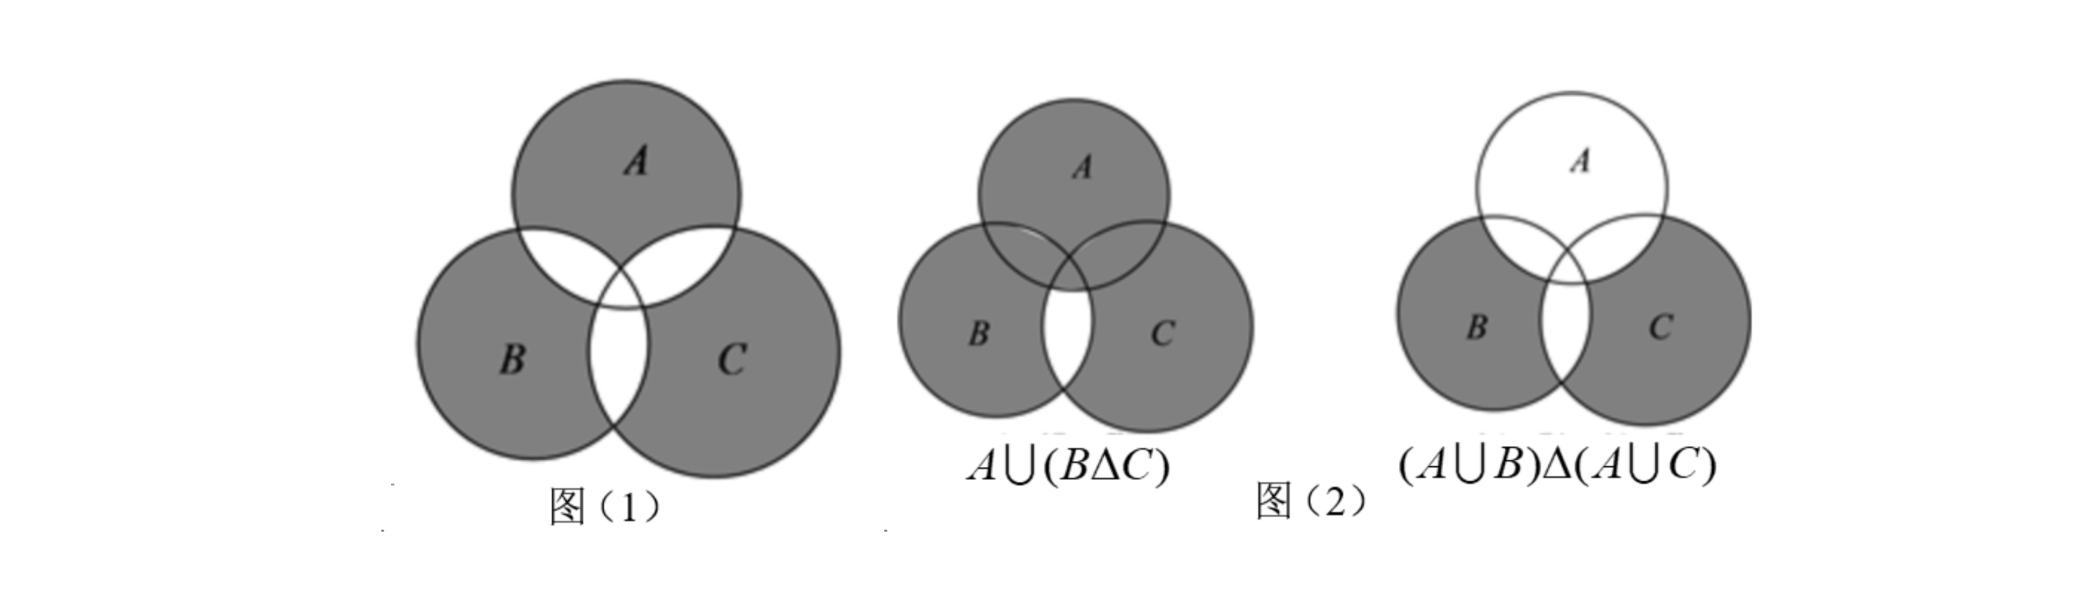
\includegraphics[width=0.92\textwidth]{figures/gao73_q16_symdiff.png}
\end{center}
\step{故选 $B$.}
\solend
\fi

\end{enumerate}

\bigsec{三、解答题}

\begin{enumerate}
\setcounter{enumi}{16}

\item （1）解不等式 $\dfrac{2-x}{x+3}>1$；

（2）已知 $a$ 是实数，试解关于 $x$ 的不等式：$x^2+(a-1)x-a\geqslant0$.

\ifanswer
\solbegin
\stepm{(1)}{$\dfrac{2-x}{x+3}-1=\dfrac{-2x-1}{x+3}>0$，则 $(2x+1)(x+3)<0$，得 $-3<x<-\dfrac12$，}
\step{所以不等式解集为 $\left(-3,-\dfrac12\right)$；}
\stepm{(2)}{$x^2+(a-1)x-a=(x+a)(x-1)\geqslant0$，}
% 原卷 (2) 题干为 ≥0，但解析按 ≤0 给出“两根之间”的解集，照录（见文件头“原卷笔误/存疑”②）
\step{当 $-a<1$，即 $a>-1$ 时，解集为 $(-a,1)$；}
\step{当 $-a=1$，即 $a=-1$ 时，解集为 $\R$；}
\step{当 $-a>1$，即 $a<-1$ 时，解集为 $(1,-a)$；}
\step{综上，当 $a>-1$ 时，解集为 $(-a,1)$；}
\step{当 $a=-1$ 时，解集为 $\R$；}
\step{当 $a<-1$ 时，解集为 $(1,-a)$.}
\solend
\fi

\ansspace[5]

\item （1）设 $a$、$b$ 是两个正数. 已知 $a>b$，比较 $\dfrac{2a+b}{a+2b}$ 与 $\dfrac ab$ 的值的大小；

（2）若实数 $a$ 满足 $\sqrt{(2023-a)^2}+\sqrt{a-2024}=a$，求 $a-2023^2$ 的值.

\ifanswer
\solbegin
\stepm{(1)}{$\dfrac{2a+b}{a+2b}-\dfrac ab=\dfrac{b^2-a^2}{b(a+2b)}<0$，所以 $\dfrac{2a+b}{a+2b}<\dfrac ab$.}
\stepm{(2)}{因为 $a-2024\geqslant0$，所以 $a\geqslant2024$，}
\step{所以 $\sqrt{(2023-a)^2}+\sqrt{a-2024}=a-2023+\sqrt{a-2024}$，}
\step{即 $a-2023+\sqrt{a-2024}=a$，即 $\sqrt{a-2024}=2023$，}
\step{所以 $a-2024=2023^2$，所以 $a-2023^2=2024$.}
\solend
\fi

\ansspace[5]

\item 已知 $m\in\R$，集合 $A=\{x\mid-1\leqslant x\leqslant3\}$，$B=\{x\mid m-3<x\leqslant m+2\}$.

（1）若“$x\in A$”是“$x\in B$”的充分不必要条件，求 $m$ 的取值范围；

（2）若 $A\cap B\neq\varnothing$，求 $m$ 的取值范围.

\ifanswer
\solbegin
\stepm{(1)}{因为“$x\in A$”是“$x\in B$”的充分不必要条件，所以 $A$ 是 $B$ 的真子集，}
\step{需满足 $\begin{cases}m-3<-1\\ m+2\geqslant3\end{cases}$，解得 $\begin{cases}m<2\\ m\geqslant1\end{cases}$，所以 $m$ 的取值范围是 $[1,2)$.}
\stepm{(2)}{因为 $A\cap B\neq\varnothing$，所以 $\begin{cases}m+2\geqslant-1\\ m-3<3\end{cases}$，解得 $\begin{cases}m\geqslant-3\\ m<6\end{cases}$，}
\step{所以 $m$ 的取值范围是 $[-3,6)$.}
\solend
\fi

\ansspace[6]

\item 已知集合 $A=\{x\mid x<-2\text{ 或 }x\geqslant3\}$，$U=\R$.

（1）若 $B=\{x\mid mx-1>0\}$，当 $B\subseteq A$ 时，求实数 $m$ 的取值范围；

（2）若 $B=\{x\mid2m-6\leqslant x\leqslant m+4\}$，当 $B\cap\overline A=\varnothing$ 时，求实数 $m$ 的取值范围.

\ifanswer
\solbegin
\stepm{(1)}{当 $m=0$ 时，$B=\varnothing$，符合题意，}
\step{当 $m>0$ 时，$B=\left\{x\mid x>\dfrac1m\right\}$，则 $\dfrac1m\geqslant3$，解得 $0<m\leqslant\dfrac13$，}
\step{当 $m<0$ 时，$B=\left\{x\mid x<\dfrac1m\right\}$，则 $\dfrac1m\leqslant-2$，解得 $-\dfrac12\leqslant m<0$，}
\step{综上所述，实数 $m$ 的取值范围 $\left[-\dfrac12,\dfrac13\right]$；}
\stepm{(2)}{由题意得 $B=\{x\mid2m-6\leqslant x\leqslant m+4\}$，$\overline A=\{x\mid-2\leqslant x<3\}$，且 $B\cap\overline A=\varnothing$，}
\step{当 $B=\varnothing$ 时，$2m-6>m+4$，解得 $m>10$，}
\step{当 $B\neq\varnothing$ 时，$\begin{cases}2m-6\leqslant m+4\\ m+4<-2\end{cases}$ 或 $\begin{cases}2m-6\leqslant m+4\\ 2m-6\geqslant3\end{cases}$，解得 $m<-6$ 或 $\dfrac92\leqslant m\leqslant10$，}
\step{综上所述，实数 $m$ 的取值范围为 $(-\infty,-6)\cup\left[\dfrac92,+\infty\right)$.}
\solend
\fi

\ansspace[7]

\item 关于实数大小关系的基本事实是解决等式或不等式问题的逻辑基础. 两个正数的大小关系是完全确定的，但通过运算就会产生非常奇妙的变化，基本不等式就是其中之一. 通过运算（代数变形）可以解决很多关于基本不等式的问题.

例如此题：正实数 $x$、$y$，满足 $x+y=1$，求 $\dfrac1x+\dfrac4y$ 的最小值. 求解本问题的方法很多，其中一种求解方法是：$\dfrac1x+\dfrac4y=(x+y)\left(\dfrac1x+\dfrac4y\right)=5+\dfrac yx+\dfrac{4x}{y}\geqslant5+2\sqrt{\dfrac yx\cdot\dfrac{4x}{y}}=9$，当且仅当 $\dfrac yx=\dfrac{4x}{y}$ 即 $y=2x$ 且 $x+y=1$ 时，即 $x=\dfrac13$，$y=\dfrac23$ 时等号成立.

这种解题方法叫作“$1$”的代换，利用上述求解方法解决下列问题：

（1）正数 $a$、$b$ 满足 $a+b=1$，求 $\dfrac1a+\dfrac2b$ 的最小值；

（2）已知 $a$、$b$、$c$ 均为正实数，且 $\dfrac1a+\dfrac1b+\dfrac1c=1$，求证：$a+b+c\geqslant9$；

（3）已知 $a$、$b$、$x$、$y$ 均为正实数，且 $\dfrac{x^2}{a^2}-\dfrac{y^2}{b^2}=1$，求证：$a^2-b^2\leqslant(x-y)^2$.

\ifanswer
\solbegin
\stepm{(1)}{正数 $a$、$b$ 满足 $a+b=1$，}
\step{$\dfrac1a+\dfrac2b=(a+b)\left(\dfrac1a+\dfrac2b\right)=1+2+\dfrac ba+\dfrac{2a}{b}\geqslant3+2\sqrt{\dfrac ba\cdot\dfrac{2a}{b}}=3+2\sqrt2$，}
\step{当且仅当 $\dfrac ba=\dfrac{2a}{b}$ 即 $b=\sqrt2\,a$ 且 $a+b=1$ 时，}
\step{即 $a=\sqrt2-1$，$b=2-\sqrt2$ 时取等号.}
\stepm{(2)}{$a+b+c=\left(\dfrac1a+\dfrac1b+\dfrac1c\right)(a+b+c)=3+\dfrac ba+\dfrac ab+\dfrac ca+\dfrac ac+\dfrac cb+\dfrac bc$}
\step{$\geqslant3+2\sqrt{\dfrac ba\cdot\dfrac ab}+2\sqrt{\dfrac ca\cdot\dfrac ac}+2\sqrt{\dfrac cb\cdot\dfrac bc}=9$，当且仅当 $a=b=c=3$ 时取等号，}
\step{故 $a+b+c\geqslant9$.}
\stepm{(3)}{$a^2-b^2=(a^2-b^2)\left(\dfrac{x^2}{a^2}-\dfrac{y^2}{b^2}\right)=x^2+y^2-\dfrac{b^2x^2}{a^2}-\dfrac{a^2y^2}{b^2}$}
\step{$=x^2+y^2-\left(\dfrac{b^2x^2}{a^2}+\dfrac{a^2y^2}{b^2}\right)\leqslant x^2+y^2-2\cdot\dfrac{bx}{a}\cdot\dfrac{ay}{b}=x^2+y^2-2xy$}
\step{$=(x-y)^2$，当且仅当 $\dfrac{bx}{a}=\dfrac{ay}{b}$ 且 $\dfrac{x^2}{a^2}-\dfrac{y^2}{b^2}=1$ 时，}
\step{即 $x=\dfrac{a^2}{\sqrt{a^2-b^2}}$，$y=\dfrac{b^2}{\sqrt{a^2-b^2}}$，$a>b$ 时取等号，故 $a^2-b^2\leqslant(x-y)^2$.}
\solend
\fi

\ansspace*[7]

\end{enumerate}

\end{document}
"
% 紧凑版：xelatex "\def\iscompact{1}% 高一73_徐汇中学_10月月考.tex
%   —— 高一上数学“2026-2027 年徐汇中学高一上 10 月月考”（讲评版）
% 试卷版：xelatex 高一73_徐汇中学_10月月考.tex
% 答案版：xelatex "\def\isanswer{1}\input{高一73_徐汇中学_10月月考.tex}"
% 紧凑版：xelatex "\def\iscompact{1}\input{高一73_徐汇中学_10月月考.tex}"
%
% 原始材料：微信公众号“魔都数学加油站”文章，连载“27学年高一73”；
% 原文标题“27学年高一73——2026-2027年上海市徐汇中学高一上10月月考”；
% 原文链接：https://mp.weixin.qq.com/s/Pkk9tFr4qHS9BR_BPxvk6A。
% 页面标注发布时间 2026-10-21 20:41（上海）。
% 正文为 10 张 PNG 页（`原图/高一73_徐汇中学_10月月考/01..10.png`）：
% 第 1、4、6、9、10 页为 2560×3620，其余 5 页为 4762×6735，均按页序读取。
% 10 页全为试卷正文页（卷首标题在第 1 页页顶，卷末第 21 题 (3) 解析止于第 10 页），
% 无封面页、目录页、二维码或宣传页。粉色斜排“魔都数学加油站”为卷面水印，未录入。
%
% 卷首标题：照卷面印作“2026-2027 年徐汇中学高一上 10 月月考”（黑体加粗一行）。
% 原卷年份区间用半角连字符，本稿按全稿惯例排 en dash；原卷无副标题。
%
% 篇幅与题号：原卷自第 3 题起编号（第 1、2 题不在本卷内）。填空题 3—12（10 题）、
% 选择题 13—16（4 题）、解答题 17—21（5 题），共 19 题。本稿沿用原节与原题号，
% 只改排为全稿统一的大节样式。
%
% 讲评版：原卷第 3、4 题只印【答案】（“没有实数根”“真”），本稿只给 \ans{}；
% 其余 17 题均印【解析】，用 \solbegin…\solend。四道选择题的作答括号原卷即留空，
% 答案写在解析末句“故选 A／D／A／B”，照录在解析内，不另提 \ans{}。
%
% 副标题：原卷未印副标题。本稿按“知识模块”口径标作“集合与常用逻辑用语、不等式”：
% 19 题中集合与常用逻辑用语 9 题（第 3、4、7、11、12、13、16、19、20 题），
% 不等式 10 题（第 5、6、8、9、10、14、15、17、18、21 题），两类均确有分量，故并标。
% 口径同 高一63、高一68—72。
%
% 与原卷的排版差异：
%   ① 原卷每题下直接印【答案】/【解析】，本稿按全稿惯例将答案与解析置于答案版；
%   ② 原卷未印副标题，本稿按“知识模块”口径补出；
%   ③ 原卷填空横线约四个字宽，本稿按全稿惯例统一排 \blankline[4.4em]；
%   ④ 原卷数集记号排斜体 $R$（第 3、8、9、10、12、17、19、20 题等），本稿按全稿惯例
%      改用 $\R$（同 高一68—72）；空集记号原卷作 $\varnothing$，照录；
%   ⑤ 原卷句末标点多为西文句点，第 15 题题干“整数解只有 $-2$”后为全角逗号，
%      均逐处照录；第 16 题解析的集合运算用 $\Delta$ 表示对称差，照原卷符号排；
%   ⑥ 第 17—21 题的子问原卷印作“（1）…（2）…”，本稿按 高一69—72 成例用行内
%      “（1）（2）（3）”段，解析中的子问标号用 \stepm{(1)}{…}；
%   ⑦ 每道解答题原卷未留作答空白，本稿按全稿惯例加 \ansspace（末题用 \ansspace*）；
%   ⑧ 选择题的作答括号原卷排半角“(    )”，本稿按全稿惯例排 \mbox{（\quad）}；
%      选项行排照原卷——第 13 题一行四条、第 14—16 题一行四条；
%   ⑨ 第 15 题题干的不等式组、第 14、19、20 题解析中的不等式组，原卷均排作“{”
%      连接的多行式，本稿按全稿惯例排 cases；
%   ⑩ 第 16 题解析末尾有三幅韦恩图（图（1）与图（2）的两幅）：原卷印在【解析】中，
%      题干无“如图”二字。本稿按原卷截图裁取（`figures/gao73_q16_symdiff.png`，
%      由第 6 页原图裁出、去除粉色水印后转灰度，未放大），放在答案版解析④之后。
%
% 原卷笔误/存疑（均照录未改，正文对应处另有 % 注）：
%   ① 第 3 题题干“设 $a$、$b\in\R$，则方程 $x^2+ax+a-1=0$ 至少有一个实根”中
%      $b$ 未在方程或后文出现，疑为衍字；原卷如此，照录未改。
%   ② 第 17 题 (2) 题干为 $x^2+(a-1)x-a\geqslant0$，但解析按 $\leqslant0$ 给出解集：
%      $a>-1$ 时写 $(-a,1)$、$a<-1$ 时写 $(1,-a)$，恰是“两根之间”的区间。
%      按题干 $\geqslant0$ 应为 $(-\infty,-a]\cup[1,+\infty)$ 与 $(-\infty,1]\cup[-a,+\infty)$；
%      原卷如此，照录未改。
%
% 行数核对：逐题数 \step/\stepm 条数与原卷【解析】印刷行数，17 题逐一相符，
% 合计 104 条 / 104 行（Q5：1；Q6：2；Q7：4；Q8：4；Q9：3；Q10：4；Q11：8；
% Q12：7；Q13：7；Q14：5；Q15：7；Q16：15；Q17：9；Q18：5；Q19：4；Q20：8；Q21：11）。
% 另第 3、4 题只印【答案】，各提 \ans{}，不计入 \step 账。
%
% 插图：第 16 题解析末的 3 幅韦恩图，见上⑩；全卷题干无其他配图。
%
\documentclass[a4paper,11pt]{article}
\usepackage{common}

\begin{document}

\examtitlest[3]{2026--2027 年徐汇中学高一上 10 月月考}{集合与常用逻辑用语、不等式}

\bigsec{一、填空题}

\begin{enumerate}
\setcounter{enumi}{2}

% 原卷题干“设 a、b∈R”中的 b 未在方程中出现，照录（见文件头“原卷笔误/存疑”①）
\item 如果用反证法证明命题“设 $a$、$b\in\R$，则方程 $x^2+ax+a-1=0$ 至少有一个实根”，那么首先假设方程 $x^2+ax+a-1=0$\blankline[4.4em].

\ifanswer
\ans{没有实数根}
\fi

\item 命题“若 $\dfrac1x>1$，则 $x<1$”是\blankline[4.4em]命题（填“真”，“假”）.

\ifanswer
\ans{真}
\fi

\item 对数 $\log_a(5-a)$ 中实数 $a$ 的取值范围是\blankline[4.4em].

\ifanswer
\solbegin
\step{由对数定义得 $\begin{cases}a>0\\ a\neq1\\ 5-a>0\end{cases}$，解得 $0<a<1$ 或 $1<a<5$.}
\solend
\fi

\item 关于 $x$ 的不等式 $ax^2-(a+1)x+1\leqslant0\,(a<0)$ 的解集为\blankline[4.4em].

\ifanswer
\solbegin
\step{原不等式即 $(ax-1)(x-1)\leqslant0$，因为 $a<0$，所以 $\left(x-\dfrac1a\right)(x-1)\geqslant0$.}
\step{又 $\dfrac1a<0<1$，所以 $x\leqslant\dfrac1a$ 或 $x\geqslant1$，故解集为 $\left(-\infty,\dfrac1a\right]\cup[1,+\infty)$.}
\solend
\fi

\item 若集合 $A=\{x\mid x^2-2kx+7k=0\}$ 有且仅有三个真子集，则 $k$ 的取值范围是\blankline[4.4em].

\ifanswer
\solbegin
\step{因为集合 $A$ 有且仅有三个真子集，则 $2^n-1=3$，解得 $n=2$，}
\step{所以一元二次方程 $x^2-2kx+7k=0$ 有两个不同的实数解，}
\step{则 $\Delta=4k^2-28k>0$，解得 $k<0$ 或 $k>7$，}
\step{故 $k$ 的取值范围是 $(-\infty,0)\cup(7,+\infty)$.}
\solend
\fi

\item 已知关于 $x$ 的不等式 $kx^2-4kx+k-6<0$ 对任意 $x\in\R$ 恒成立，则 $k$ 的取值范围是\blankline[4.4em].

\ifanswer
\solbegin
\step{关于 $x$ 的不等式 $kx^2-4kx+k-6<0$ 对任意 $x\in\R$ 恒成立，}
\step{当 $k=0$ 时，$kx^2-4kx+k-6=-6<0$ 恒成立，}
\step{当 $k\neq0$ 时，则 $\begin{cases}\Delta=16k^2-4k(k-6)<0\\ k<0\end{cases}$，解得 $-2<k<0$，}
\step{综上，$k$ 的取值范围为 $(-2,0]$.}
\solend
\fi

\item 设 $x\in\R$，方程 $|x-1|+|2x-1|=|3x-2|$ 的解集为\blankline[4.4em].

\ifanswer
\solbegin
\step{因为 $|x-1|+|2x-1|\geqslant|(x-1)+(2x-1)|=|3x-2|$，}
\step{当且仅当 $(x-1)(2x-1)\geqslant0$，解得 $x\leqslant\dfrac12$ 或 $x\geqslant1$，}
\step{故方程 $|x-1|+|2x-1|=|3x-2|$ 的解集为 $\left(-\infty,\dfrac12\right]\cup[1,+\infty)$.}
\solend
\fi

\item 已知 $a\in\R$，若关于 $x$ 的方程 $x^2+ax+a^2-8=0$ 有两个实根 $x_1$、$x_2$，且 $\dfrac1{x_1}+\dfrac1{x_2}=-\dfrac12$，则 $a$ 的值为\blankline[4.4em].

\ifanswer
\solbegin
\step{由题意得 $\Delta=a^2-4(a^2-8)=32-3a^2\geqslant0$，解得 $a^2\leqslant\dfrac{32}3$，}
\step{由韦达定理得 $x_1+x_2=-a$，$x_1x_2=a^2-8$，}
\step{则 $\dfrac1{x_1}+\dfrac1{x_2}=\dfrac{x_1+x_2}{x_1x_2}=\dfrac{-a}{a^2-8}=-\dfrac12$，即 $a^2-2a-8=(a-4)(a+2)=0$，}
\step{解得 $a=4$ 或 $a=-2$. 又 $a^2\leqslant\dfrac{32}3$，则 $a=-2$.}
\solend
\fi

\item 甲、乙两人解关于 $x$ 的不等式 $x^2+bx+c<0$，甲写错了 $b$，正确计算后得到的解为 $\{x\mid1<x<2\}$；乙写错了 $c$，正确计算后得到的解为 $\{x\mid-4<x<1\}$. 那么不等式 $\dfrac{bx+c}{x-2}<0$ 的解为\blankline[4.4em].

\ifanswer
\solbegin
\step{由 $x^2+bx+c<0$ 的解为 $\{x\mid1<x<2\}$，}
\step{则 $1$ 和 $2$ 是方程 $x^2+bx+c=0$ 的两个根，}
\step{甲写错了 $b$，但 $c$ 是正确的，所以 $c=1\times2=2$；}
\step{由 $x^2+bx+c<0$ 的解为 $\{x\mid-4<x<1\}$，}
\step{则 $-4$ 和 $1$ 是方程 $x^2+bx+c=0$ 的两个根，}
\step{乙写错了 $c$，但 $b$ 是正确的，所以 $-b=-4+1=-3$，即 $b=3$.}
\step{由 $\dfrac{bx+c}{x-2}<0$，得 $\dfrac{3x+2}{x-2}<0$，即 $(3x+2)(x-2)<0$，解得 $-\dfrac23<x<2$，}
\step{所以不等式 $\dfrac{bx+c}{x-2}<0$ 的解为 $\left\{x\mid-\dfrac23<x<2\right\}$.}
\solend
\fi

\item 设 $a,b,c\in\R$，$S=\{x\mid(x+a)(x^2+bx+c)=0,x\in\R\}$，$T=\{x\mid(ax+1)(cx^2+bx+1)=0,x\in\R\}$. 若 $|S|$、$|T|$ 分别为集合 $S$、$T$ 的元素个数，则 $|S|+|T|$ 的所有可能取值组成的集合为\blankline[4.4em].

\ifanswer
\solbegin
\step{$x\neq0$ 时，$(ax+1)(cx^2+bx+1)=x^3\left(\dfrac1x+a\right)\left(\dfrac1{x^2}+\dfrac bx+c\right)$，}
\step{故 $S$、$T$ 的非零元按倒数一一对应，设其个数均为 $k$；}
\step{$0\notin T$，且 $0\in S\Leftrightarrow ac=0$. 当 $ac=0$ 时 $k\in\{0,1,2\}$，}
\step{当 $ac\neq0$ 时 $x=-a\neq0$ 是 $S$ 的非零元，$k\in\{1,2,3\}$.}
\step{因此 $|S|+|T|$ 分别可取 $2k+1\in\{1,3,5\}$ 与 $2k\in\{2,4,6\}$.}
\step{依次取 $(a,b,c)=(0,0,0),(1,0,1),(0,-2,1),(1,-2,1),(0,0,-1),(1,-5,6)$，可分别实现 $1,2,3,4,5,6$，}
\step{则 $|S|+|T|$ 的所有可能取值组成的集合为 $\{1,2,3,4,5,6\}$.}
\solend
\fi

\end{enumerate}

\bigsec{二、选择题}

\begin{enumerate}
\setcounter{enumi}{12}

\item 如果 $a>b$，$c\neq0$，那么下列不等式成立的是\mbox{（\quad）}

\keepwithprev
A. $a-c>b-c$\qquad B. $c-a>c-b$\qquad C. $ac>bc$\qquad D. $\dfrac ac>\dfrac bc$

\ifanswer
\solbegin
\step{对于 $A$：$a-c-(b-c)=a-b>0$，即 $a-c>b-c$，故 $A$ 正确；}
\step{对于 $B$：$c-a-(c-b)=b-a<0$，即 $c-a<c-b$，故 $B$ 错误；}
\step{对于 $C$：$ac-bc=c(a-b)$，已知 $a-b>0$，}
\step{当 $c<0$ 时，$c(a-b)<0$，此时 $ac<bc$，故 $C$ 错误；}
\step{对于 $D$：$\dfrac ac-\dfrac bc=\dfrac1c(a-b)$，已知 $a-b>0$，}
\step{当 $c<0$ 时，$\dfrac1c(a-b)<0$，此时 $\dfrac ac<\dfrac bc$，故 $D$ 错误.}
\step{故选 $A$.}
\solend
\fi

\item 若不等式 $|x+1|\leqslant a$ 成立的一个充分不必要条件是 $-3\leqslant x\leqslant4$，则整数 $a$ 的最小值为\mbox{（\quad）}

\keepwithprev
A. $2$\qquad B. $3$\qquad C. $4$\qquad D. $5$

\ifanswer
\solbegin
\step{若 $a<0$，则 $|x+1|\leqslant a$ 无解；}
\step{若 $a\geqslant0$，由 $|x+1|\leqslant a$，得 $-1-a\leqslant x\leqslant-1+a$，}
\step{因为 $|x+1|\leqslant a$ 成立的一个充分不必要条件是 $-3\leqslant x\leqslant4$，}
\step{所以 $\begin{cases}-1-a\leqslant-3\\ -1+a\geqslant4\end{cases}$，等号不同时成立，解得 $a\geqslant5$，}
\step{故整数 $a$ 的最小值为 $5$. 故选 $D$.}
\solend
\fi

\item 若关于 $x$ 的不等式组 $\begin{cases}x^2-x-2>0\\ 2x^2+(5+2k)x+5k<0\end{cases}$ 的整数解只有 $-2$，则实数 $k$ 的取值范围为\mbox{（\quad）}

\keepwithprev
A. $[-3,2)$\qquad B. $[1,2]$\qquad C. $(1,2]$\qquad D. $(1,2)$

\ifanswer
\solbegin
\step{由 $x^2-x-2>0$，得 $x>2$ 或 $x<-1$，}
\step{由 $2x^2+(2k+5)x+5k<0$，得 $(2x+5)(x+k)<0$.}
\step{①若 $-k<-\dfrac52$，即 $k>\dfrac52$ 时，解得 $-k<x<-\dfrac52$，}
\step{此时原不等式的解集为 $\left(-k,-\dfrac52\right)$，不符合题意；}
\step{②若 $k=\dfrac52$ 时，解得 $x\in\varnothing$，显然不符合题意；}
\step{③若 $k<\dfrac52$ 时，解得 $-\dfrac52<x<-k$，则 $-2<-k\leqslant3$，即 $-3\leqslant k<2$.}
\step{综上，实数 $k$ 的取值范围 $[-3,2)$. 故选 $A$.}
\solend
\fi

\item 定义集合运算 $A-B=\{x\mid x\in A\text{ 且 }x\notin B\}$ 称为集合 $A$ 与集合 $B$ 的差集；定义集合运算 $A\Delta B=(A-B)\cup(B-A)$ 称为集合 $A$ 与集合 $B$ 的对称差，有以下 $4$ 个等式：

① $A\Delta B=B\Delta A$；

② $(A\Delta B)\Delta C=A\Delta(B\Delta C)$；

③ $A\cap(B\Delta C)=(A\cap B)\Delta(A\cap C)$；

④ $A\cup(B\Delta C)=(A\cup B)\Delta(A\cup C)$.

则 $4$ 个等式中恒成立的是\mbox{（\quad）}

\keepwithprev
A. ①②\qquad B. ①②③\qquad C. ①②④\qquad D. ①②③④

\ifanswer
\solbegin
\step{对于①，由 $B\Delta A=(B-A)\cup(A-B)=(A-B)\cup(B-A)=A\Delta B$，}
\step{所以①正确；}
\step{对于②，}
\step{由 $A-B=\{x\mid x\in A\text{ 且 }x\notin B\}=\{x\mid x\in A,x\notin(A\cap B)\}=A-(A\cap B)$，}
\step{同理可得 $B-A=B-(A\cap B)$，}
\step{则 $A\Delta B=(A-B)\cup(B-A)=(A\cup B)-(A\cap B)$，}
\step{所以 $(A\Delta B)\Delta C=(A\Delta B)\cup C-(A\Delta B)\cap C$，}
\step{所以表示的集合为图（1）中阴影部分所表示的集合，如图所示，}
\step{同理 $A\Delta(B\Delta C)=A\cup(B\Delta C)-A\cap(B\Delta C)$，}
\step{也表示图（1）中阴影部分所表示的集合，}
\step{所以 $(A\Delta B)\Delta C=A\Delta(B\Delta C)$，所以②正确；}
\step{对于③，由 $A\cap(B\Delta C)=A\cap(B\cup C-B\cap C)=A\cap(B\cup C)-A\cap(B\cap C)$}
\step{$=(A\cap B)\cup(A\cap C)-(A\cap B)\cap(A\cap C)=(A\cap B)\Delta(A\cap C)$，所以③正确；}
\step{对于④，如图（2）所示，$A\cup(B\Delta C)\neq(A\cup B)\Delta(A\cup C)$，所以④错误.}
\begin{center}
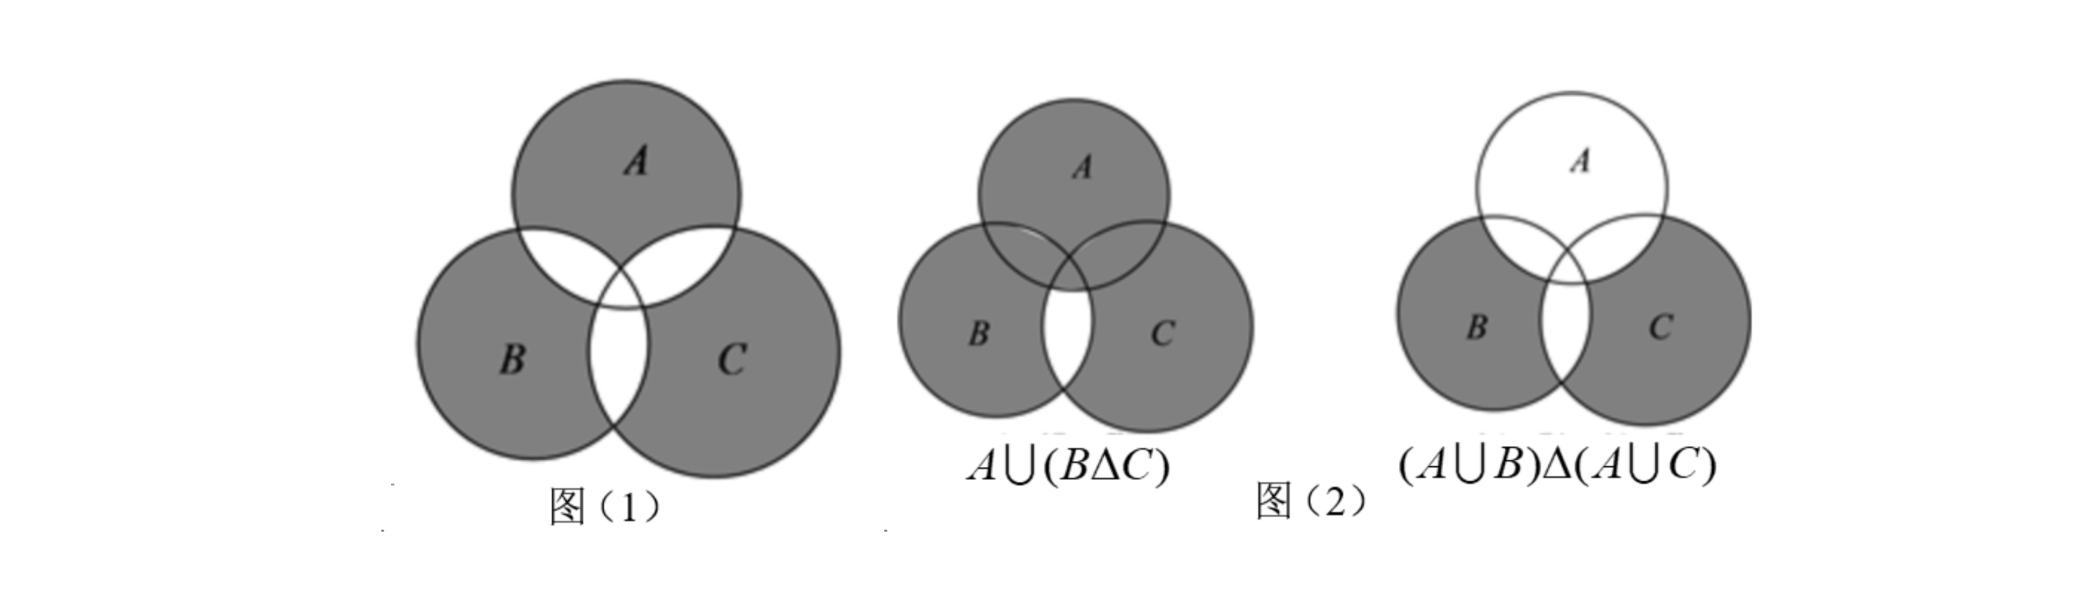
\includegraphics[width=0.92\textwidth]{figures/gao73_q16_symdiff.png}
\end{center}
\step{故选 $B$.}
\solend
\fi

\end{enumerate}

\bigsec{三、解答题}

\begin{enumerate}
\setcounter{enumi}{16}

\item （1）解不等式 $\dfrac{2-x}{x+3}>1$；

（2）已知 $a$ 是实数，试解关于 $x$ 的不等式：$x^2+(a-1)x-a\geqslant0$.

\ifanswer
\solbegin
\stepm{(1)}{$\dfrac{2-x}{x+3}-1=\dfrac{-2x-1}{x+3}>0$，则 $(2x+1)(x+3)<0$，得 $-3<x<-\dfrac12$，}
\step{所以不等式解集为 $\left(-3,-\dfrac12\right)$；}
\stepm{(2)}{$x^2+(a-1)x-a=(x+a)(x-1)\geqslant0$，}
% 原卷 (2) 题干为 ≥0，但解析按 ≤0 给出“两根之间”的解集，照录（见文件头“原卷笔误/存疑”②）
\step{当 $-a<1$，即 $a>-1$ 时，解集为 $(-a,1)$；}
\step{当 $-a=1$，即 $a=-1$ 时，解集为 $\R$；}
\step{当 $-a>1$，即 $a<-1$ 时，解集为 $(1,-a)$；}
\step{综上，当 $a>-1$ 时，解集为 $(-a,1)$；}
\step{当 $a=-1$ 时，解集为 $\R$；}
\step{当 $a<-1$ 时，解集为 $(1,-a)$.}
\solend
\fi

\ansspace[5]

\item （1）设 $a$、$b$ 是两个正数. 已知 $a>b$，比较 $\dfrac{2a+b}{a+2b}$ 与 $\dfrac ab$ 的值的大小；

（2）若实数 $a$ 满足 $\sqrt{(2023-a)^2}+\sqrt{a-2024}=a$，求 $a-2023^2$ 的值.

\ifanswer
\solbegin
\stepm{(1)}{$\dfrac{2a+b}{a+2b}-\dfrac ab=\dfrac{b^2-a^2}{b(a+2b)}<0$，所以 $\dfrac{2a+b}{a+2b}<\dfrac ab$.}
\stepm{(2)}{因为 $a-2024\geqslant0$，所以 $a\geqslant2024$，}
\step{所以 $\sqrt{(2023-a)^2}+\sqrt{a-2024}=a-2023+\sqrt{a-2024}$，}
\step{即 $a-2023+\sqrt{a-2024}=a$，即 $\sqrt{a-2024}=2023$，}
\step{所以 $a-2024=2023^2$，所以 $a-2023^2=2024$.}
\solend
\fi

\ansspace[5]

\item 已知 $m\in\R$，集合 $A=\{x\mid-1\leqslant x\leqslant3\}$，$B=\{x\mid m-3<x\leqslant m+2\}$.

（1）若“$x\in A$”是“$x\in B$”的充分不必要条件，求 $m$ 的取值范围；

（2）若 $A\cap B\neq\varnothing$，求 $m$ 的取值范围.

\ifanswer
\solbegin
\stepm{(1)}{因为“$x\in A$”是“$x\in B$”的充分不必要条件，所以 $A$ 是 $B$ 的真子集，}
\step{需满足 $\begin{cases}m-3<-1\\ m+2\geqslant3\end{cases}$，解得 $\begin{cases}m<2\\ m\geqslant1\end{cases}$，所以 $m$ 的取值范围是 $[1,2)$.}
\stepm{(2)}{因为 $A\cap B\neq\varnothing$，所以 $\begin{cases}m+2\geqslant-1\\ m-3<3\end{cases}$，解得 $\begin{cases}m\geqslant-3\\ m<6\end{cases}$，}
\step{所以 $m$ 的取值范围是 $[-3,6)$.}
\solend
\fi

\ansspace[6]

\item 已知集合 $A=\{x\mid x<-2\text{ 或 }x\geqslant3\}$，$U=\R$.

（1）若 $B=\{x\mid mx-1>0\}$，当 $B\subseteq A$ 时，求实数 $m$ 的取值范围；

（2）若 $B=\{x\mid2m-6\leqslant x\leqslant m+4\}$，当 $B\cap\overline A=\varnothing$ 时，求实数 $m$ 的取值范围.

\ifanswer
\solbegin
\stepm{(1)}{当 $m=0$ 时，$B=\varnothing$，符合题意，}
\step{当 $m>0$ 时，$B=\left\{x\mid x>\dfrac1m\right\}$，则 $\dfrac1m\geqslant3$，解得 $0<m\leqslant\dfrac13$，}
\step{当 $m<0$ 时，$B=\left\{x\mid x<\dfrac1m\right\}$，则 $\dfrac1m\leqslant-2$，解得 $-\dfrac12\leqslant m<0$，}
\step{综上所述，实数 $m$ 的取值范围 $\left[-\dfrac12,\dfrac13\right]$；}
\stepm{(2)}{由题意得 $B=\{x\mid2m-6\leqslant x\leqslant m+4\}$，$\overline A=\{x\mid-2\leqslant x<3\}$，且 $B\cap\overline A=\varnothing$，}
\step{当 $B=\varnothing$ 时，$2m-6>m+4$，解得 $m>10$，}
\step{当 $B\neq\varnothing$ 时，$\begin{cases}2m-6\leqslant m+4\\ m+4<-2\end{cases}$ 或 $\begin{cases}2m-6\leqslant m+4\\ 2m-6\geqslant3\end{cases}$，解得 $m<-6$ 或 $\dfrac92\leqslant m\leqslant10$，}
\step{综上所述，实数 $m$ 的取值范围为 $(-\infty,-6)\cup\left[\dfrac92,+\infty\right)$.}
\solend
\fi

\ansspace[7]

\item 关于实数大小关系的基本事实是解决等式或不等式问题的逻辑基础. 两个正数的大小关系是完全确定的，但通过运算就会产生非常奇妙的变化，基本不等式就是其中之一. 通过运算（代数变形）可以解决很多关于基本不等式的问题.

例如此题：正实数 $x$、$y$，满足 $x+y=1$，求 $\dfrac1x+\dfrac4y$ 的最小值. 求解本问题的方法很多，其中一种求解方法是：$\dfrac1x+\dfrac4y=(x+y)\left(\dfrac1x+\dfrac4y\right)=5+\dfrac yx+\dfrac{4x}{y}\geqslant5+2\sqrt{\dfrac yx\cdot\dfrac{4x}{y}}=9$，当且仅当 $\dfrac yx=\dfrac{4x}{y}$ 即 $y=2x$ 且 $x+y=1$ 时，即 $x=\dfrac13$，$y=\dfrac23$ 时等号成立.

这种解题方法叫作“$1$”的代换，利用上述求解方法解决下列问题：

（1）正数 $a$、$b$ 满足 $a+b=1$，求 $\dfrac1a+\dfrac2b$ 的最小值；

（2）已知 $a$、$b$、$c$ 均为正实数，且 $\dfrac1a+\dfrac1b+\dfrac1c=1$，求证：$a+b+c\geqslant9$；

（3）已知 $a$、$b$、$x$、$y$ 均为正实数，且 $\dfrac{x^2}{a^2}-\dfrac{y^2}{b^2}=1$，求证：$a^2-b^2\leqslant(x-y)^2$.

\ifanswer
\solbegin
\stepm{(1)}{正数 $a$、$b$ 满足 $a+b=1$，}
\step{$\dfrac1a+\dfrac2b=(a+b)\left(\dfrac1a+\dfrac2b\right)=1+2+\dfrac ba+\dfrac{2a}{b}\geqslant3+2\sqrt{\dfrac ba\cdot\dfrac{2a}{b}}=3+2\sqrt2$，}
\step{当且仅当 $\dfrac ba=\dfrac{2a}{b}$ 即 $b=\sqrt2\,a$ 且 $a+b=1$ 时，}
\step{即 $a=\sqrt2-1$，$b=2-\sqrt2$ 时取等号.}
\stepm{(2)}{$a+b+c=\left(\dfrac1a+\dfrac1b+\dfrac1c\right)(a+b+c)=3+\dfrac ba+\dfrac ab+\dfrac ca+\dfrac ac+\dfrac cb+\dfrac bc$}
\step{$\geqslant3+2\sqrt{\dfrac ba\cdot\dfrac ab}+2\sqrt{\dfrac ca\cdot\dfrac ac}+2\sqrt{\dfrac cb\cdot\dfrac bc}=9$，当且仅当 $a=b=c=3$ 时取等号，}
\step{故 $a+b+c\geqslant9$.}
\stepm{(3)}{$a^2-b^2=(a^2-b^2)\left(\dfrac{x^2}{a^2}-\dfrac{y^2}{b^2}\right)=x^2+y^2-\dfrac{b^2x^2}{a^2}-\dfrac{a^2y^2}{b^2}$}
\step{$=x^2+y^2-\left(\dfrac{b^2x^2}{a^2}+\dfrac{a^2y^2}{b^2}\right)\leqslant x^2+y^2-2\cdot\dfrac{bx}{a}\cdot\dfrac{ay}{b}=x^2+y^2-2xy$}
\step{$=(x-y)^2$，当且仅当 $\dfrac{bx}{a}=\dfrac{ay}{b}$ 且 $\dfrac{x^2}{a^2}-\dfrac{y^2}{b^2}=1$ 时，}
\step{即 $x=\dfrac{a^2}{\sqrt{a^2-b^2}}$，$y=\dfrac{b^2}{\sqrt{a^2-b^2}}$，$a>b$ 时取等号，故 $a^2-b^2\leqslant(x-y)^2$.}
\solend
\fi

\ansspace*[7]

\end{enumerate}

\end{document}
"
%
% 原始材料：微信公众号“魔都数学加油站”文章，连载“27学年高一73”；
% 原文标题“27学年高一73——2026-2027年上海市徐汇中学高一上10月月考”；
% 原文链接：https://mp.weixin.qq.com/s/Pkk9tFr4qHS9BR_BPxvk6A。
% 页面标注发布时间 2026-10-21 20:41（上海）。
% 正文为 10 张 PNG 页（`原图/高一73_徐汇中学_10月月考/01..10.png`）：
% 第 1、4、6、9、10 页为 2560×3620，其余 5 页为 4762×6735，均按页序读取。
% 10 页全为试卷正文页（卷首标题在第 1 页页顶，卷末第 21 题 (3) 解析止于第 10 页），
% 无封面页、目录页、二维码或宣传页。粉色斜排“魔都数学加油站”为卷面水印，未录入。
%
% 卷首标题：照卷面印作“2026-2027 年徐汇中学高一上 10 月月考”（黑体加粗一行）。
% 原卷年份区间用半角连字符，本稿按全稿惯例排 en dash；原卷无副标题。
%
% 篇幅与题号：原卷自第 3 题起编号（第 1、2 题不在本卷内）。填空题 3—12（10 题）、
% 选择题 13—16（4 题）、解答题 17—21（5 题），共 19 题。本稿沿用原节与原题号，
% 只改排为全稿统一的大节样式。
%
% 讲评版：原卷第 3、4 题只印【答案】（“没有实数根”“真”），本稿只给 \ans{}；
% 其余 17 题均印【解析】，用 \solbegin…\solend。四道选择题的作答括号原卷即留空，
% 答案写在解析末句“故选 A／D／A／B”，照录在解析内，不另提 \ans{}。
%
% 副标题：原卷未印副标题。本稿按“知识模块”口径标作“集合与常用逻辑用语、不等式”：
% 19 题中集合与常用逻辑用语 9 题（第 3、4、7、11、12、13、16、19、20 题），
% 不等式 10 题（第 5、6、8、9、10、14、15、17、18、21 题），两类均确有分量，故并标。
% 口径同 高一63、高一68—72。
%
% 与原卷的排版差异：
%   ① 原卷每题下直接印【答案】/【解析】，本稿按全稿惯例将答案与解析置于答案版；
%   ② 原卷未印副标题，本稿按“知识模块”口径补出；
%   ③ 原卷填空横线约四个字宽，本稿按全稿惯例统一排 \blankline[4.4em]；
%   ④ 原卷数集记号排斜体 $R$（第 3、8、9、10、12、17、19、20 题等），本稿按全稿惯例
%      改用 $\R$（同 高一68—72）；空集记号原卷作 $\varnothing$，照录；
%   ⑤ 原卷句末标点多为西文句点，第 15 题题干“整数解只有 $-2$”后为全角逗号，
%      均逐处照录；第 16 题解析的集合运算用 $\Delta$ 表示对称差，照原卷符号排；
%   ⑥ 第 17—21 题的子问原卷印作“（1）…（2）…”，本稿按 高一69—72 成例用行内
%      “（1）（2）（3）”段，解析中的子问标号用 \stepm{(1)}{…}；
%   ⑦ 每道解答题原卷未留作答空白，本稿按全稿惯例加 \ansspace（末题用 \ansspace*）；
%   ⑧ 选择题的作答括号原卷排半角“(    )”，本稿按全稿惯例排 \mbox{（\quad）}；
%      选项行排照原卷——第 13 题一行四条、第 14—16 题一行四条；
%   ⑨ 第 15 题题干的不等式组、第 14、19、20 题解析中的不等式组，原卷均排作“{”
%      连接的多行式，本稿按全稿惯例排 cases；
%   ⑩ 第 16 题解析末尾有三幅韦恩图（图（1）与图（2）的两幅）：原卷印在【解析】中，
%      题干无“如图”二字。本稿按原卷截图裁取（`figures/gao73_q16_symdiff.png`，
%      由第 6 页原图裁出、去除粉色水印后转灰度，未放大），放在答案版解析④之后。
%
% 原卷笔误/存疑（均照录未改，正文对应处另有 % 注）：
%   ① 第 3 题题干“设 $a$、$b\in\R$，则方程 $x^2+ax+a-1=0$ 至少有一个实根”中
%      $b$ 未在方程或后文出现，疑为衍字；原卷如此，照录未改。
%   ② 第 17 题 (2) 题干为 $x^2+(a-1)x-a\geqslant0$，但解析按 $\leqslant0$ 给出解集：
%      $a>-1$ 时写 $(-a,1)$、$a<-1$ 时写 $(1,-a)$，恰是“两根之间”的区间。
%      按题干 $\geqslant0$ 应为 $(-\infty,-a]\cup[1,+\infty)$ 与 $(-\infty,1]\cup[-a,+\infty)$；
%      原卷如此，照录未改。
%
% 行数核对：逐题数 \step/\stepm 条数与原卷【解析】印刷行数，17 题逐一相符，
% 合计 104 条 / 104 行（Q5：1；Q6：2；Q7：4；Q8：4；Q9：3；Q10：4；Q11：8；
% Q12：7；Q13：7；Q14：5；Q15：7；Q16：15；Q17：9；Q18：5；Q19：4；Q20：8；Q21：11）。
% 另第 3、4 题只印【答案】，各提 \ans{}，不计入 \step 账。
%
% 插图：第 16 题解析末的 3 幅韦恩图，见上⑩；全卷题干无其他配图。
%
\documentclass[a4paper,11pt]{article}
\usepackage{common}

\begin{document}

\examtitlest[3]{2026--2027 年徐汇中学高一上 10 月月考}{集合与常用逻辑用语、不等式}

\bigsec{一、填空题}

\begin{enumerate}
\setcounter{enumi}{2}

% 原卷题干“设 a、b∈R”中的 b 未在方程中出现，照录（见文件头“原卷笔误/存疑”①）
\item 如果用反证法证明命题“设 $a$、$b\in\R$，则方程 $x^2+ax+a-1=0$ 至少有一个实根”，那么首先假设方程 $x^2+ax+a-1=0$\blankline[4.4em].

\ifanswer
\ans{没有实数根}
\fi

\item 命题“若 $\dfrac1x>1$，则 $x<1$”是\blankline[4.4em]命题（填“真”，“假”）.

\ifanswer
\ans{真}
\fi

\item 对数 $\log_a(5-a)$ 中实数 $a$ 的取值范围是\blankline[4.4em].

\ifanswer
\solbegin
\step{由对数定义得 $\begin{cases}a>0\\ a\neq1\\ 5-a>0\end{cases}$，解得 $0<a<1$ 或 $1<a<5$.}
\solend
\fi

\item 关于 $x$ 的不等式 $ax^2-(a+1)x+1\leqslant0\,(a<0)$ 的解集为\blankline[4.4em].

\ifanswer
\solbegin
\step{原不等式即 $(ax-1)(x-1)\leqslant0$，因为 $a<0$，所以 $\left(x-\dfrac1a\right)(x-1)\geqslant0$.}
\step{又 $\dfrac1a<0<1$，所以 $x\leqslant\dfrac1a$ 或 $x\geqslant1$，故解集为 $\left(-\infty,\dfrac1a\right]\cup[1,+\infty)$.}
\solend
\fi

\item 若集合 $A=\{x\mid x^2-2kx+7k=0\}$ 有且仅有三个真子集，则 $k$ 的取值范围是\blankline[4.4em].

\ifanswer
\solbegin
\step{因为集合 $A$ 有且仅有三个真子集，则 $2^n-1=3$，解得 $n=2$，}
\step{所以一元二次方程 $x^2-2kx+7k=0$ 有两个不同的实数解，}
\step{则 $\Delta=4k^2-28k>0$，解得 $k<0$ 或 $k>7$，}
\step{故 $k$ 的取值范围是 $(-\infty,0)\cup(7,+\infty)$.}
\solend
\fi

\item 已知关于 $x$ 的不等式 $kx^2-4kx+k-6<0$ 对任意 $x\in\R$ 恒成立，则 $k$ 的取值范围是\blankline[4.4em].

\ifanswer
\solbegin
\step{关于 $x$ 的不等式 $kx^2-4kx+k-6<0$ 对任意 $x\in\R$ 恒成立，}
\step{当 $k=0$ 时，$kx^2-4kx+k-6=-6<0$ 恒成立，}
\step{当 $k\neq0$ 时，则 $\begin{cases}\Delta=16k^2-4k(k-6)<0\\ k<0\end{cases}$，解得 $-2<k<0$，}
\step{综上，$k$ 的取值范围为 $(-2,0]$.}
\solend
\fi

\item 设 $x\in\R$，方程 $|x-1|+|2x-1|=|3x-2|$ 的解集为\blankline[4.4em].

\ifanswer
\solbegin
\step{因为 $|x-1|+|2x-1|\geqslant|(x-1)+(2x-1)|=|3x-2|$，}
\step{当且仅当 $(x-1)(2x-1)\geqslant0$，解得 $x\leqslant\dfrac12$ 或 $x\geqslant1$，}
\step{故方程 $|x-1|+|2x-1|=|3x-2|$ 的解集为 $\left(-\infty,\dfrac12\right]\cup[1,+\infty)$.}
\solend
\fi

\item 已知 $a\in\R$，若关于 $x$ 的方程 $x^2+ax+a^2-8=0$ 有两个实根 $x_1$、$x_2$，且 $\dfrac1{x_1}+\dfrac1{x_2}=-\dfrac12$，则 $a$ 的值为\blankline[4.4em].

\ifanswer
\solbegin
\step{由题意得 $\Delta=a^2-4(a^2-8)=32-3a^2\geqslant0$，解得 $a^2\leqslant\dfrac{32}3$，}
\step{由韦达定理得 $x_1+x_2=-a$，$x_1x_2=a^2-8$，}
\step{则 $\dfrac1{x_1}+\dfrac1{x_2}=\dfrac{x_1+x_2}{x_1x_2}=\dfrac{-a}{a^2-8}=-\dfrac12$，即 $a^2-2a-8=(a-4)(a+2)=0$，}
\step{解得 $a=4$ 或 $a=-2$. 又 $a^2\leqslant\dfrac{32}3$，则 $a=-2$.}
\solend
\fi

\item 甲、乙两人解关于 $x$ 的不等式 $x^2+bx+c<0$，甲写错了 $b$，正确计算后得到的解为 $\{x\mid1<x<2\}$；乙写错了 $c$，正确计算后得到的解为 $\{x\mid-4<x<1\}$. 那么不等式 $\dfrac{bx+c}{x-2}<0$ 的解为\blankline[4.4em].

\ifanswer
\solbegin
\step{由 $x^2+bx+c<0$ 的解为 $\{x\mid1<x<2\}$，}
\step{则 $1$ 和 $2$ 是方程 $x^2+bx+c=0$ 的两个根，}
\step{甲写错了 $b$，但 $c$ 是正确的，所以 $c=1\times2=2$；}
\step{由 $x^2+bx+c<0$ 的解为 $\{x\mid-4<x<1\}$，}
\step{则 $-4$ 和 $1$ 是方程 $x^2+bx+c=0$ 的两个根，}
\step{乙写错了 $c$，但 $b$ 是正确的，所以 $-b=-4+1=-3$，即 $b=3$.}
\step{由 $\dfrac{bx+c}{x-2}<0$，得 $\dfrac{3x+2}{x-2}<0$，即 $(3x+2)(x-2)<0$，解得 $-\dfrac23<x<2$，}
\step{所以不等式 $\dfrac{bx+c}{x-2}<0$ 的解为 $\left\{x\mid-\dfrac23<x<2\right\}$.}
\solend
\fi

\item 设 $a,b,c\in\R$，$S=\{x\mid(x+a)(x^2+bx+c)=0,x\in\R\}$，$T=\{x\mid(ax+1)(cx^2+bx+1)=0,x\in\R\}$. 若 $|S|$、$|T|$ 分别为集合 $S$、$T$ 的元素个数，则 $|S|+|T|$ 的所有可能取值组成的集合为\blankline[4.4em].

\ifanswer
\solbegin
\step{$x\neq0$ 时，$(ax+1)(cx^2+bx+1)=x^3\left(\dfrac1x+a\right)\left(\dfrac1{x^2}+\dfrac bx+c\right)$，}
\step{故 $S$、$T$ 的非零元按倒数一一对应，设其个数均为 $k$；}
\step{$0\notin T$，且 $0\in S\Leftrightarrow ac=0$. 当 $ac=0$ 时 $k\in\{0,1,2\}$，}
\step{当 $ac\neq0$ 时 $x=-a\neq0$ 是 $S$ 的非零元，$k\in\{1,2,3\}$.}
\step{因此 $|S|+|T|$ 分别可取 $2k+1\in\{1,3,5\}$ 与 $2k\in\{2,4,6\}$.}
\step{依次取 $(a,b,c)=(0,0,0),(1,0,1),(0,-2,1),(1,-2,1),(0,0,-1),(1,-5,6)$，可分别实现 $1,2,3,4,5,6$，}
\step{则 $|S|+|T|$ 的所有可能取值组成的集合为 $\{1,2,3,4,5,6\}$.}
\solend
\fi

\end{enumerate}

\bigsec{二、选择题}

\begin{enumerate}
\setcounter{enumi}{12}

\item 如果 $a>b$，$c\neq0$，那么下列不等式成立的是\mbox{（\quad）}

\keepwithprev
A. $a-c>b-c$\qquad B. $c-a>c-b$\qquad C. $ac>bc$\qquad D. $\dfrac ac>\dfrac bc$

\ifanswer
\solbegin
\step{对于 $A$：$a-c-(b-c)=a-b>0$，即 $a-c>b-c$，故 $A$ 正确；}
\step{对于 $B$：$c-a-(c-b)=b-a<0$，即 $c-a<c-b$，故 $B$ 错误；}
\step{对于 $C$：$ac-bc=c(a-b)$，已知 $a-b>0$，}
\step{当 $c<0$ 时，$c(a-b)<0$，此时 $ac<bc$，故 $C$ 错误；}
\step{对于 $D$：$\dfrac ac-\dfrac bc=\dfrac1c(a-b)$，已知 $a-b>0$，}
\step{当 $c<0$ 时，$\dfrac1c(a-b)<0$，此时 $\dfrac ac<\dfrac bc$，故 $D$ 错误.}
\step{故选 $A$.}
\solend
\fi

\item 若不等式 $|x+1|\leqslant a$ 成立的一个充分不必要条件是 $-3\leqslant x\leqslant4$，则整数 $a$ 的最小值为\mbox{（\quad）}

\keepwithprev
A. $2$\qquad B. $3$\qquad C. $4$\qquad D. $5$

\ifanswer
\solbegin
\step{若 $a<0$，则 $|x+1|\leqslant a$ 无解；}
\step{若 $a\geqslant0$，由 $|x+1|\leqslant a$，得 $-1-a\leqslant x\leqslant-1+a$，}
\step{因为 $|x+1|\leqslant a$ 成立的一个充分不必要条件是 $-3\leqslant x\leqslant4$，}
\step{所以 $\begin{cases}-1-a\leqslant-3\\ -1+a\geqslant4\end{cases}$，等号不同时成立，解得 $a\geqslant5$，}
\step{故整数 $a$ 的最小值为 $5$. 故选 $D$.}
\solend
\fi

\item 若关于 $x$ 的不等式组 $\begin{cases}x^2-x-2>0\\ 2x^2+(5+2k)x+5k<0\end{cases}$ 的整数解只有 $-2$，则实数 $k$ 的取值范围为\mbox{（\quad）}

\keepwithprev
A. $[-3,2)$\qquad B. $[1,2]$\qquad C. $(1,2]$\qquad D. $(1,2)$

\ifanswer
\solbegin
\step{由 $x^2-x-2>0$，得 $x>2$ 或 $x<-1$，}
\step{由 $2x^2+(2k+5)x+5k<0$，得 $(2x+5)(x+k)<0$.}
\step{①若 $-k<-\dfrac52$，即 $k>\dfrac52$ 时，解得 $-k<x<-\dfrac52$，}
\step{此时原不等式的解集为 $\left(-k,-\dfrac52\right)$，不符合题意；}
\step{②若 $k=\dfrac52$ 时，解得 $x\in\varnothing$，显然不符合题意；}
\step{③若 $k<\dfrac52$ 时，解得 $-\dfrac52<x<-k$，则 $-2<-k\leqslant3$，即 $-3\leqslant k<2$.}
\step{综上，实数 $k$ 的取值范围 $[-3,2)$. 故选 $A$.}
\solend
\fi

\item 定义集合运算 $A-B=\{x\mid x\in A\text{ 且 }x\notin B\}$ 称为集合 $A$ 与集合 $B$ 的差集；定义集合运算 $A\Delta B=(A-B)\cup(B-A)$ 称为集合 $A$ 与集合 $B$ 的对称差，有以下 $4$ 个等式：

① $A\Delta B=B\Delta A$；

② $(A\Delta B)\Delta C=A\Delta(B\Delta C)$；

③ $A\cap(B\Delta C)=(A\cap B)\Delta(A\cap C)$；

④ $A\cup(B\Delta C)=(A\cup B)\Delta(A\cup C)$.

则 $4$ 个等式中恒成立的是\mbox{（\quad）}

\keepwithprev
A. ①②\qquad B. ①②③\qquad C. ①②④\qquad D. ①②③④

\ifanswer
\solbegin
\step{对于①，由 $B\Delta A=(B-A)\cup(A-B)=(A-B)\cup(B-A)=A\Delta B$，}
\step{所以①正确；}
\step{对于②，}
\step{由 $A-B=\{x\mid x\in A\text{ 且 }x\notin B\}=\{x\mid x\in A,x\notin(A\cap B)\}=A-(A\cap B)$，}
\step{同理可得 $B-A=B-(A\cap B)$，}
\step{则 $A\Delta B=(A-B)\cup(B-A)=(A\cup B)-(A\cap B)$，}
\step{所以 $(A\Delta B)\Delta C=(A\Delta B)\cup C-(A\Delta B)\cap C$，}
\step{所以表示的集合为图（1）中阴影部分所表示的集合，如图所示，}
\step{同理 $A\Delta(B\Delta C)=A\cup(B\Delta C)-A\cap(B\Delta C)$，}
\step{也表示图（1）中阴影部分所表示的集合，}
\step{所以 $(A\Delta B)\Delta C=A\Delta(B\Delta C)$，所以②正确；}
\step{对于③，由 $A\cap(B\Delta C)=A\cap(B\cup C-B\cap C)=A\cap(B\cup C)-A\cap(B\cap C)$}
\step{$=(A\cap B)\cup(A\cap C)-(A\cap B)\cap(A\cap C)=(A\cap B)\Delta(A\cap C)$，所以③正确；}
\step{对于④，如图（2）所示，$A\cup(B\Delta C)\neq(A\cup B)\Delta(A\cup C)$，所以④错误.}
\begin{center}
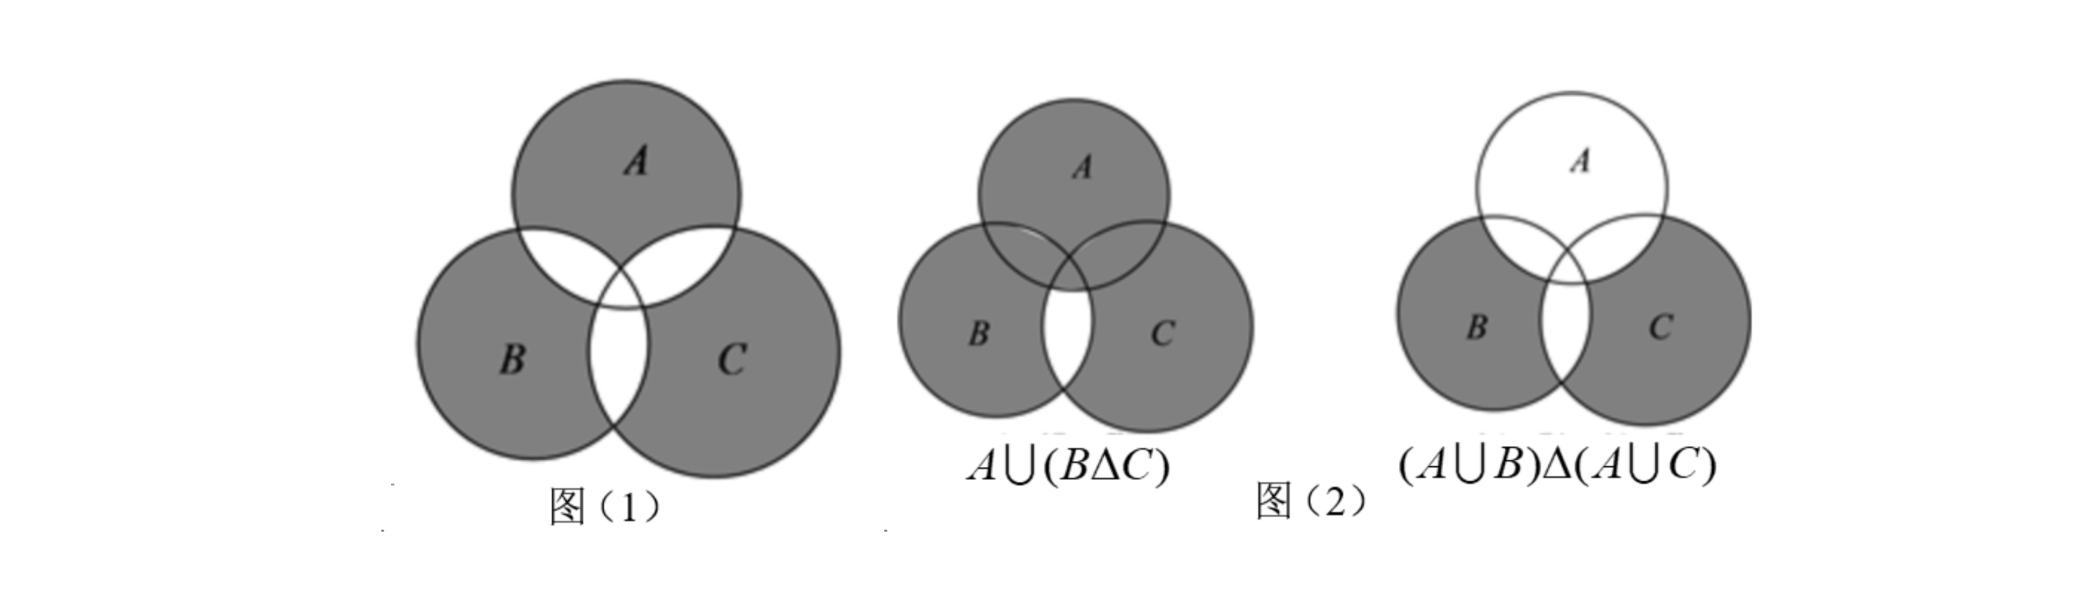
\includegraphics[width=0.92\textwidth]{figures/gao73_q16_symdiff.png}
\end{center}
\step{故选 $B$.}
\solend
\fi

\end{enumerate}

\bigsec{三、解答题}

\begin{enumerate}
\setcounter{enumi}{16}

\item （1）解不等式 $\dfrac{2-x}{x+3}>1$；

（2）已知 $a$ 是实数，试解关于 $x$ 的不等式：$x^2+(a-1)x-a\geqslant0$.

\ifanswer
\solbegin
\stepm{(1)}{$\dfrac{2-x}{x+3}-1=\dfrac{-2x-1}{x+3}>0$，则 $(2x+1)(x+3)<0$，得 $-3<x<-\dfrac12$，}
\step{所以不等式解集为 $\left(-3,-\dfrac12\right)$；}
\stepm{(2)}{$x^2+(a-1)x-a=(x+a)(x-1)\geqslant0$，}
% 原卷 (2) 题干为 ≥0，但解析按 ≤0 给出“两根之间”的解集，照录（见文件头“原卷笔误/存疑”②）
\step{当 $-a<1$，即 $a>-1$ 时，解集为 $(-a,1)$；}
\step{当 $-a=1$，即 $a=-1$ 时，解集为 $\R$；}
\step{当 $-a>1$，即 $a<-1$ 时，解集为 $(1,-a)$；}
\step{综上，当 $a>-1$ 时，解集为 $(-a,1)$；}
\step{当 $a=-1$ 时，解集为 $\R$；}
\step{当 $a<-1$ 时，解集为 $(1,-a)$.}
\solend
\fi

\ansspace[5]

\item （1）设 $a$、$b$ 是两个正数. 已知 $a>b$，比较 $\dfrac{2a+b}{a+2b}$ 与 $\dfrac ab$ 的值的大小；

（2）若实数 $a$ 满足 $\sqrt{(2023-a)^2}+\sqrt{a-2024}=a$，求 $a-2023^2$ 的值.

\ifanswer
\solbegin
\stepm{(1)}{$\dfrac{2a+b}{a+2b}-\dfrac ab=\dfrac{b^2-a^2}{b(a+2b)}<0$，所以 $\dfrac{2a+b}{a+2b}<\dfrac ab$.}
\stepm{(2)}{因为 $a-2024\geqslant0$，所以 $a\geqslant2024$，}
\step{所以 $\sqrt{(2023-a)^2}+\sqrt{a-2024}=a-2023+\sqrt{a-2024}$，}
\step{即 $a-2023+\sqrt{a-2024}=a$，即 $\sqrt{a-2024}=2023$，}
\step{所以 $a-2024=2023^2$，所以 $a-2023^2=2024$.}
\solend
\fi

\ansspace[5]

\item 已知 $m\in\R$，集合 $A=\{x\mid-1\leqslant x\leqslant3\}$，$B=\{x\mid m-3<x\leqslant m+2\}$.

（1）若“$x\in A$”是“$x\in B$”的充分不必要条件，求 $m$ 的取值范围；

（2）若 $A\cap B\neq\varnothing$，求 $m$ 的取值范围.

\ifanswer
\solbegin
\stepm{(1)}{因为“$x\in A$”是“$x\in B$”的充分不必要条件，所以 $A$ 是 $B$ 的真子集，}
\step{需满足 $\begin{cases}m-3<-1\\ m+2\geqslant3\end{cases}$，解得 $\begin{cases}m<2\\ m\geqslant1\end{cases}$，所以 $m$ 的取值范围是 $[1,2)$.}
\stepm{(2)}{因为 $A\cap B\neq\varnothing$，所以 $\begin{cases}m+2\geqslant-1\\ m-3<3\end{cases}$，解得 $\begin{cases}m\geqslant-3\\ m<6\end{cases}$，}
\step{所以 $m$ 的取值范围是 $[-3,6)$.}
\solend
\fi

\ansspace[6]

\item 已知集合 $A=\{x\mid x<-2\text{ 或 }x\geqslant3\}$，$U=\R$.

（1）若 $B=\{x\mid mx-1>0\}$，当 $B\subseteq A$ 时，求实数 $m$ 的取值范围；

（2）若 $B=\{x\mid2m-6\leqslant x\leqslant m+4\}$，当 $B\cap\overline A=\varnothing$ 时，求实数 $m$ 的取值范围.

\ifanswer
\solbegin
\stepm{(1)}{当 $m=0$ 时，$B=\varnothing$，符合题意，}
\step{当 $m>0$ 时，$B=\left\{x\mid x>\dfrac1m\right\}$，则 $\dfrac1m\geqslant3$，解得 $0<m\leqslant\dfrac13$，}
\step{当 $m<0$ 时，$B=\left\{x\mid x<\dfrac1m\right\}$，则 $\dfrac1m\leqslant-2$，解得 $-\dfrac12\leqslant m<0$，}
\step{综上所述，实数 $m$ 的取值范围 $\left[-\dfrac12,\dfrac13\right]$；}
\stepm{(2)}{由题意得 $B=\{x\mid2m-6\leqslant x\leqslant m+4\}$，$\overline A=\{x\mid-2\leqslant x<3\}$，且 $B\cap\overline A=\varnothing$，}
\step{当 $B=\varnothing$ 时，$2m-6>m+4$，解得 $m>10$，}
\step{当 $B\neq\varnothing$ 时，$\begin{cases}2m-6\leqslant m+4\\ m+4<-2\end{cases}$ 或 $\begin{cases}2m-6\leqslant m+4\\ 2m-6\geqslant3\end{cases}$，解得 $m<-6$ 或 $\dfrac92\leqslant m\leqslant10$，}
\step{综上所述，实数 $m$ 的取值范围为 $(-\infty,-6)\cup\left[\dfrac92,+\infty\right)$.}
\solend
\fi

\ansspace[7]

\item 关于实数大小关系的基本事实是解决等式或不等式问题的逻辑基础. 两个正数的大小关系是完全确定的，但通过运算就会产生非常奇妙的变化，基本不等式就是其中之一. 通过运算（代数变形）可以解决很多关于基本不等式的问题.

例如此题：正实数 $x$、$y$，满足 $x+y=1$，求 $\dfrac1x+\dfrac4y$ 的最小值. 求解本问题的方法很多，其中一种求解方法是：$\dfrac1x+\dfrac4y=(x+y)\left(\dfrac1x+\dfrac4y\right)=5+\dfrac yx+\dfrac{4x}{y}\geqslant5+2\sqrt{\dfrac yx\cdot\dfrac{4x}{y}}=9$，当且仅当 $\dfrac yx=\dfrac{4x}{y}$ 即 $y=2x$ 且 $x+y=1$ 时，即 $x=\dfrac13$，$y=\dfrac23$ 时等号成立.

这种解题方法叫作“$1$”的代换，利用上述求解方法解决下列问题：

（1）正数 $a$、$b$ 满足 $a+b=1$，求 $\dfrac1a+\dfrac2b$ 的最小值；

（2）已知 $a$、$b$、$c$ 均为正实数，且 $\dfrac1a+\dfrac1b+\dfrac1c=1$，求证：$a+b+c\geqslant9$；

（3）已知 $a$、$b$、$x$、$y$ 均为正实数，且 $\dfrac{x^2}{a^2}-\dfrac{y^2}{b^2}=1$，求证：$a^2-b^2\leqslant(x-y)^2$.

\ifanswer
\solbegin
\stepm{(1)}{正数 $a$、$b$ 满足 $a+b=1$，}
\step{$\dfrac1a+\dfrac2b=(a+b)\left(\dfrac1a+\dfrac2b\right)=1+2+\dfrac ba+\dfrac{2a}{b}\geqslant3+2\sqrt{\dfrac ba\cdot\dfrac{2a}{b}}=3+2\sqrt2$，}
\step{当且仅当 $\dfrac ba=\dfrac{2a}{b}$ 即 $b=\sqrt2\,a$ 且 $a+b=1$ 时，}
\step{即 $a=\sqrt2-1$，$b=2-\sqrt2$ 时取等号.}
\stepm{(2)}{$a+b+c=\left(\dfrac1a+\dfrac1b+\dfrac1c\right)(a+b+c)=3+\dfrac ba+\dfrac ab+\dfrac ca+\dfrac ac+\dfrac cb+\dfrac bc$}
\step{$\geqslant3+2\sqrt{\dfrac ba\cdot\dfrac ab}+2\sqrt{\dfrac ca\cdot\dfrac ac}+2\sqrt{\dfrac cb\cdot\dfrac bc}=9$，当且仅当 $a=b=c=3$ 时取等号，}
\step{故 $a+b+c\geqslant9$.}
\stepm{(3)}{$a^2-b^2=(a^2-b^2)\left(\dfrac{x^2}{a^2}-\dfrac{y^2}{b^2}\right)=x^2+y^2-\dfrac{b^2x^2}{a^2}-\dfrac{a^2y^2}{b^2}$}
\step{$=x^2+y^2-\left(\dfrac{b^2x^2}{a^2}+\dfrac{a^2y^2}{b^2}\right)\leqslant x^2+y^2-2\cdot\dfrac{bx}{a}\cdot\dfrac{ay}{b}=x^2+y^2-2xy$}
\step{$=(x-y)^2$，当且仅当 $\dfrac{bx}{a}=\dfrac{ay}{b}$ 且 $\dfrac{x^2}{a^2}-\dfrac{y^2}{b^2}=1$ 时，}
\step{即 $x=\dfrac{a^2}{\sqrt{a^2-b^2}}$，$y=\dfrac{b^2}{\sqrt{a^2-b^2}}$，$a>b$ 时取等号，故 $a^2-b^2\leqslant(x-y)^2$.}
\solend
\fi

\ansspace*[7]

\end{enumerate}

\end{document}
"
% 紧凑版：xelatex "\def\iscompact{1}% 高一73_徐汇中学_10月月考.tex
%   —— 高一上数学“2026-2027 年徐汇中学高一上 10 月月考”（讲评版）
% 试卷版：xelatex 高一73_徐汇中学_10月月考.tex
% 答案版：xelatex "\def\isanswer{1}% 高一73_徐汇中学_10月月考.tex
%   —— 高一上数学“2026-2027 年徐汇中学高一上 10 月月考”（讲评版）
% 试卷版：xelatex 高一73_徐汇中学_10月月考.tex
% 答案版：xelatex "\def\isanswer{1}\input{高一73_徐汇中学_10月月考.tex}"
% 紧凑版：xelatex "\def\iscompact{1}\input{高一73_徐汇中学_10月月考.tex}"
%
% 原始材料：微信公众号“魔都数学加油站”文章，连载“27学年高一73”；
% 原文标题“27学年高一73——2026-2027年上海市徐汇中学高一上10月月考”；
% 原文链接：https://mp.weixin.qq.com/s/Pkk9tFr4qHS9BR_BPxvk6A。
% 页面标注发布时间 2026-10-21 20:41（上海）。
% 正文为 10 张 PNG 页（`原图/高一73_徐汇中学_10月月考/01..10.png`）：
% 第 1、4、6、9、10 页为 2560×3620，其余 5 页为 4762×6735，均按页序读取。
% 10 页全为试卷正文页（卷首标题在第 1 页页顶，卷末第 21 题 (3) 解析止于第 10 页），
% 无封面页、目录页、二维码或宣传页。粉色斜排“魔都数学加油站”为卷面水印，未录入。
%
% 卷首标题：照卷面印作“2026-2027 年徐汇中学高一上 10 月月考”（黑体加粗一行）。
% 原卷年份区间用半角连字符，本稿按全稿惯例排 en dash；原卷无副标题。
%
% 篇幅与题号：原卷自第 3 题起编号（第 1、2 题不在本卷内）。填空题 3—12（10 题）、
% 选择题 13—16（4 题）、解答题 17—21（5 题），共 19 题。本稿沿用原节与原题号，
% 只改排为全稿统一的大节样式。
%
% 讲评版：原卷第 3、4 题只印【答案】（“没有实数根”“真”），本稿只给 \ans{}；
% 其余 17 题均印【解析】，用 \solbegin…\solend。四道选择题的作答括号原卷即留空，
% 答案写在解析末句“故选 A／D／A／B”，照录在解析内，不另提 \ans{}。
%
% 副标题：原卷未印副标题。本稿按“知识模块”口径标作“集合与常用逻辑用语、不等式”：
% 19 题中集合与常用逻辑用语 9 题（第 3、4、7、11、12、13、16、19、20 题），
% 不等式 10 题（第 5、6、8、9、10、14、15、17、18、21 题），两类均确有分量，故并标。
% 口径同 高一63、高一68—72。
%
% 与原卷的排版差异：
%   ① 原卷每题下直接印【答案】/【解析】，本稿按全稿惯例将答案与解析置于答案版；
%   ② 原卷未印副标题，本稿按“知识模块”口径补出；
%   ③ 原卷填空横线约四个字宽，本稿按全稿惯例统一排 \blankline[4.4em]；
%   ④ 原卷数集记号排斜体 $R$（第 3、8、9、10、12、17、19、20 题等），本稿按全稿惯例
%      改用 $\R$（同 高一68—72）；空集记号原卷作 $\varnothing$，照录；
%   ⑤ 原卷句末标点多为西文句点，第 15 题题干“整数解只有 $-2$”后为全角逗号，
%      均逐处照录；第 16 题解析的集合运算用 $\Delta$ 表示对称差，照原卷符号排；
%   ⑥ 第 17—21 题的子问原卷印作“（1）…（2）…”，本稿按 高一69—72 成例用行内
%      “（1）（2）（3）”段，解析中的子问标号用 \stepm{(1)}{…}；
%   ⑦ 每道解答题原卷未留作答空白，本稿按全稿惯例加 \ansspace（末题用 \ansspace*）；
%   ⑧ 选择题的作答括号原卷排半角“(    )”，本稿按全稿惯例排 \mbox{（\quad）}；
%      选项行排照原卷——第 13 题一行四条、第 14—16 题一行四条；
%   ⑨ 第 15 题题干的不等式组、第 14、19、20 题解析中的不等式组，原卷均排作“{”
%      连接的多行式，本稿按全稿惯例排 cases；
%   ⑩ 第 16 题解析末尾有三幅韦恩图（图（1）与图（2）的两幅）：原卷印在【解析】中，
%      题干无“如图”二字。本稿按原卷截图裁取（`figures/gao73_q16_symdiff.png`，
%      由第 6 页原图裁出、去除粉色水印后转灰度，未放大），放在答案版解析④之后。
%
% 原卷笔误/存疑（均照录未改，正文对应处另有 % 注）：
%   ① 第 3 题题干“设 $a$、$b\in\R$，则方程 $x^2+ax+a-1=0$ 至少有一个实根”中
%      $b$ 未在方程或后文出现，疑为衍字；原卷如此，照录未改。
%   ② 第 17 题 (2) 题干为 $x^2+(a-1)x-a\geqslant0$，但解析按 $\leqslant0$ 给出解集：
%      $a>-1$ 时写 $(-a,1)$、$a<-1$ 时写 $(1,-a)$，恰是“两根之间”的区间。
%      按题干 $\geqslant0$ 应为 $(-\infty,-a]\cup[1,+\infty)$ 与 $(-\infty,1]\cup[-a,+\infty)$；
%      原卷如此，照录未改。
%
% 行数核对：逐题数 \step/\stepm 条数与原卷【解析】印刷行数，17 题逐一相符，
% 合计 104 条 / 104 行（Q5：1；Q6：2；Q7：4；Q8：4；Q9：3；Q10：4；Q11：8；
% Q12：7；Q13：7；Q14：5；Q15：7；Q16：15；Q17：9；Q18：5；Q19：4；Q20：8；Q21：11）。
% 另第 3、4 题只印【答案】，各提 \ans{}，不计入 \step 账。
%
% 插图：第 16 题解析末的 3 幅韦恩图，见上⑩；全卷题干无其他配图。
%
\documentclass[a4paper,11pt]{article}
\usepackage{common}

\begin{document}

\examtitlest[3]{2026--2027 年徐汇中学高一上 10 月月考}{集合与常用逻辑用语、不等式}

\bigsec{一、填空题}

\begin{enumerate}
\setcounter{enumi}{2}

% 原卷题干“设 a、b∈R”中的 b 未在方程中出现，照录（见文件头“原卷笔误/存疑”①）
\item 如果用反证法证明命题“设 $a$、$b\in\R$，则方程 $x^2+ax+a-1=0$ 至少有一个实根”，那么首先假设方程 $x^2+ax+a-1=0$\blankline[4.4em].

\ifanswer
\ans{没有实数根}
\fi

\item 命题“若 $\dfrac1x>1$，则 $x<1$”是\blankline[4.4em]命题（填“真”，“假”）.

\ifanswer
\ans{真}
\fi

\item 对数 $\log_a(5-a)$ 中实数 $a$ 的取值范围是\blankline[4.4em].

\ifanswer
\solbegin
\step{由对数定义得 $\begin{cases}a>0\\ a\neq1\\ 5-a>0\end{cases}$，解得 $0<a<1$ 或 $1<a<5$.}
\solend
\fi

\item 关于 $x$ 的不等式 $ax^2-(a+1)x+1\leqslant0\,(a<0)$ 的解集为\blankline[4.4em].

\ifanswer
\solbegin
\step{原不等式即 $(ax-1)(x-1)\leqslant0$，因为 $a<0$，所以 $\left(x-\dfrac1a\right)(x-1)\geqslant0$.}
\step{又 $\dfrac1a<0<1$，所以 $x\leqslant\dfrac1a$ 或 $x\geqslant1$，故解集为 $\left(-\infty,\dfrac1a\right]\cup[1,+\infty)$.}
\solend
\fi

\item 若集合 $A=\{x\mid x^2-2kx+7k=0\}$ 有且仅有三个真子集，则 $k$ 的取值范围是\blankline[4.4em].

\ifanswer
\solbegin
\step{因为集合 $A$ 有且仅有三个真子集，则 $2^n-1=3$，解得 $n=2$，}
\step{所以一元二次方程 $x^2-2kx+7k=0$ 有两个不同的实数解，}
\step{则 $\Delta=4k^2-28k>0$，解得 $k<0$ 或 $k>7$，}
\step{故 $k$ 的取值范围是 $(-\infty,0)\cup(7,+\infty)$.}
\solend
\fi

\item 已知关于 $x$ 的不等式 $kx^2-4kx+k-6<0$ 对任意 $x\in\R$ 恒成立，则 $k$ 的取值范围是\blankline[4.4em].

\ifanswer
\solbegin
\step{关于 $x$ 的不等式 $kx^2-4kx+k-6<0$ 对任意 $x\in\R$ 恒成立，}
\step{当 $k=0$ 时，$kx^2-4kx+k-6=-6<0$ 恒成立，}
\step{当 $k\neq0$ 时，则 $\begin{cases}\Delta=16k^2-4k(k-6)<0\\ k<0\end{cases}$，解得 $-2<k<0$，}
\step{综上，$k$ 的取值范围为 $(-2,0]$.}
\solend
\fi

\item 设 $x\in\R$，方程 $|x-1|+|2x-1|=|3x-2|$ 的解集为\blankline[4.4em].

\ifanswer
\solbegin
\step{因为 $|x-1|+|2x-1|\geqslant|(x-1)+(2x-1)|=|3x-2|$，}
\step{当且仅当 $(x-1)(2x-1)\geqslant0$，解得 $x\leqslant\dfrac12$ 或 $x\geqslant1$，}
\step{故方程 $|x-1|+|2x-1|=|3x-2|$ 的解集为 $\left(-\infty,\dfrac12\right]\cup[1,+\infty)$.}
\solend
\fi

\item 已知 $a\in\R$，若关于 $x$ 的方程 $x^2+ax+a^2-8=0$ 有两个实根 $x_1$、$x_2$，且 $\dfrac1{x_1}+\dfrac1{x_2}=-\dfrac12$，则 $a$ 的值为\blankline[4.4em].

\ifanswer
\solbegin
\step{由题意得 $\Delta=a^2-4(a^2-8)=32-3a^2\geqslant0$，解得 $a^2\leqslant\dfrac{32}3$，}
\step{由韦达定理得 $x_1+x_2=-a$，$x_1x_2=a^2-8$，}
\step{则 $\dfrac1{x_1}+\dfrac1{x_2}=\dfrac{x_1+x_2}{x_1x_2}=\dfrac{-a}{a^2-8}=-\dfrac12$，即 $a^2-2a-8=(a-4)(a+2)=0$，}
\step{解得 $a=4$ 或 $a=-2$. 又 $a^2\leqslant\dfrac{32}3$，则 $a=-2$.}
\solend
\fi

\item 甲、乙两人解关于 $x$ 的不等式 $x^2+bx+c<0$，甲写错了 $b$，正确计算后得到的解为 $\{x\mid1<x<2\}$；乙写错了 $c$，正确计算后得到的解为 $\{x\mid-4<x<1\}$. 那么不等式 $\dfrac{bx+c}{x-2}<0$ 的解为\blankline[4.4em].

\ifanswer
\solbegin
\step{由 $x^2+bx+c<0$ 的解为 $\{x\mid1<x<2\}$，}
\step{则 $1$ 和 $2$ 是方程 $x^2+bx+c=0$ 的两个根，}
\step{甲写错了 $b$，但 $c$ 是正确的，所以 $c=1\times2=2$；}
\step{由 $x^2+bx+c<0$ 的解为 $\{x\mid-4<x<1\}$，}
\step{则 $-4$ 和 $1$ 是方程 $x^2+bx+c=0$ 的两个根，}
\step{乙写错了 $c$，但 $b$ 是正确的，所以 $-b=-4+1=-3$，即 $b=3$.}
\step{由 $\dfrac{bx+c}{x-2}<0$，得 $\dfrac{3x+2}{x-2}<0$，即 $(3x+2)(x-2)<0$，解得 $-\dfrac23<x<2$，}
\step{所以不等式 $\dfrac{bx+c}{x-2}<0$ 的解为 $\left\{x\mid-\dfrac23<x<2\right\}$.}
\solend
\fi

\item 设 $a,b,c\in\R$，$S=\{x\mid(x+a)(x^2+bx+c)=0,x\in\R\}$，$T=\{x\mid(ax+1)(cx^2+bx+1)=0,x\in\R\}$. 若 $|S|$、$|T|$ 分别为集合 $S$、$T$ 的元素个数，则 $|S|+|T|$ 的所有可能取值组成的集合为\blankline[4.4em].

\ifanswer
\solbegin
\step{$x\neq0$ 时，$(ax+1)(cx^2+bx+1)=x^3\left(\dfrac1x+a\right)\left(\dfrac1{x^2}+\dfrac bx+c\right)$，}
\step{故 $S$、$T$ 的非零元按倒数一一对应，设其个数均为 $k$；}
\step{$0\notin T$，且 $0\in S\Leftrightarrow ac=0$. 当 $ac=0$ 时 $k\in\{0,1,2\}$，}
\step{当 $ac\neq0$ 时 $x=-a\neq0$ 是 $S$ 的非零元，$k\in\{1,2,3\}$.}
\step{因此 $|S|+|T|$ 分别可取 $2k+1\in\{1,3,5\}$ 与 $2k\in\{2,4,6\}$.}
\step{依次取 $(a,b,c)=(0,0,0),(1,0,1),(0,-2,1),(1,-2,1),(0,0,-1),(1,-5,6)$，可分别实现 $1,2,3,4,5,6$，}
\step{则 $|S|+|T|$ 的所有可能取值组成的集合为 $\{1,2,3,4,5,6\}$.}
\solend
\fi

\end{enumerate}

\bigsec{二、选择题}

\begin{enumerate}
\setcounter{enumi}{12}

\item 如果 $a>b$，$c\neq0$，那么下列不等式成立的是\mbox{（\quad）}

\keepwithprev
A. $a-c>b-c$\qquad B. $c-a>c-b$\qquad C. $ac>bc$\qquad D. $\dfrac ac>\dfrac bc$

\ifanswer
\solbegin
\step{对于 $A$：$a-c-(b-c)=a-b>0$，即 $a-c>b-c$，故 $A$ 正确；}
\step{对于 $B$：$c-a-(c-b)=b-a<0$，即 $c-a<c-b$，故 $B$ 错误；}
\step{对于 $C$：$ac-bc=c(a-b)$，已知 $a-b>0$，}
\step{当 $c<0$ 时，$c(a-b)<0$，此时 $ac<bc$，故 $C$ 错误；}
\step{对于 $D$：$\dfrac ac-\dfrac bc=\dfrac1c(a-b)$，已知 $a-b>0$，}
\step{当 $c<0$ 时，$\dfrac1c(a-b)<0$，此时 $\dfrac ac<\dfrac bc$，故 $D$ 错误.}
\step{故选 $A$.}
\solend
\fi

\item 若不等式 $|x+1|\leqslant a$ 成立的一个充分不必要条件是 $-3\leqslant x\leqslant4$，则整数 $a$ 的最小值为\mbox{（\quad）}

\keepwithprev
A. $2$\qquad B. $3$\qquad C. $4$\qquad D. $5$

\ifanswer
\solbegin
\step{若 $a<0$，则 $|x+1|\leqslant a$ 无解；}
\step{若 $a\geqslant0$，由 $|x+1|\leqslant a$，得 $-1-a\leqslant x\leqslant-1+a$，}
\step{因为 $|x+1|\leqslant a$ 成立的一个充分不必要条件是 $-3\leqslant x\leqslant4$，}
\step{所以 $\begin{cases}-1-a\leqslant-3\\ -1+a\geqslant4\end{cases}$，等号不同时成立，解得 $a\geqslant5$，}
\step{故整数 $a$ 的最小值为 $5$. 故选 $D$.}
\solend
\fi

\item 若关于 $x$ 的不等式组 $\begin{cases}x^2-x-2>0\\ 2x^2+(5+2k)x+5k<0\end{cases}$ 的整数解只有 $-2$，则实数 $k$ 的取值范围为\mbox{（\quad）}

\keepwithprev
A. $[-3,2)$\qquad B. $[1,2]$\qquad C. $(1,2]$\qquad D. $(1,2)$

\ifanswer
\solbegin
\step{由 $x^2-x-2>0$，得 $x>2$ 或 $x<-1$，}
\step{由 $2x^2+(2k+5)x+5k<0$，得 $(2x+5)(x+k)<0$.}
\step{①若 $-k<-\dfrac52$，即 $k>\dfrac52$ 时，解得 $-k<x<-\dfrac52$，}
\step{此时原不等式的解集为 $\left(-k,-\dfrac52\right)$，不符合题意；}
\step{②若 $k=\dfrac52$ 时，解得 $x\in\varnothing$，显然不符合题意；}
\step{③若 $k<\dfrac52$ 时，解得 $-\dfrac52<x<-k$，则 $-2<-k\leqslant3$，即 $-3\leqslant k<2$.}
\step{综上，实数 $k$ 的取值范围 $[-3,2)$. 故选 $A$.}
\solend
\fi

\item 定义集合运算 $A-B=\{x\mid x\in A\text{ 且 }x\notin B\}$ 称为集合 $A$ 与集合 $B$ 的差集；定义集合运算 $A\Delta B=(A-B)\cup(B-A)$ 称为集合 $A$ 与集合 $B$ 的对称差，有以下 $4$ 个等式：

① $A\Delta B=B\Delta A$；

② $(A\Delta B)\Delta C=A\Delta(B\Delta C)$；

③ $A\cap(B\Delta C)=(A\cap B)\Delta(A\cap C)$；

④ $A\cup(B\Delta C)=(A\cup B)\Delta(A\cup C)$.

则 $4$ 个等式中恒成立的是\mbox{（\quad）}

\keepwithprev
A. ①②\qquad B. ①②③\qquad C. ①②④\qquad D. ①②③④

\ifanswer
\solbegin
\step{对于①，由 $B\Delta A=(B-A)\cup(A-B)=(A-B)\cup(B-A)=A\Delta B$，}
\step{所以①正确；}
\step{对于②，}
\step{由 $A-B=\{x\mid x\in A\text{ 且 }x\notin B\}=\{x\mid x\in A,x\notin(A\cap B)\}=A-(A\cap B)$，}
\step{同理可得 $B-A=B-(A\cap B)$，}
\step{则 $A\Delta B=(A-B)\cup(B-A)=(A\cup B)-(A\cap B)$，}
\step{所以 $(A\Delta B)\Delta C=(A\Delta B)\cup C-(A\Delta B)\cap C$，}
\step{所以表示的集合为图（1）中阴影部分所表示的集合，如图所示，}
\step{同理 $A\Delta(B\Delta C)=A\cup(B\Delta C)-A\cap(B\Delta C)$，}
\step{也表示图（1）中阴影部分所表示的集合，}
\step{所以 $(A\Delta B)\Delta C=A\Delta(B\Delta C)$，所以②正确；}
\step{对于③，由 $A\cap(B\Delta C)=A\cap(B\cup C-B\cap C)=A\cap(B\cup C)-A\cap(B\cap C)$}
\step{$=(A\cap B)\cup(A\cap C)-(A\cap B)\cap(A\cap C)=(A\cap B)\Delta(A\cap C)$，所以③正确；}
\step{对于④，如图（2）所示，$A\cup(B\Delta C)\neq(A\cup B)\Delta(A\cup C)$，所以④错误.}
\begin{center}
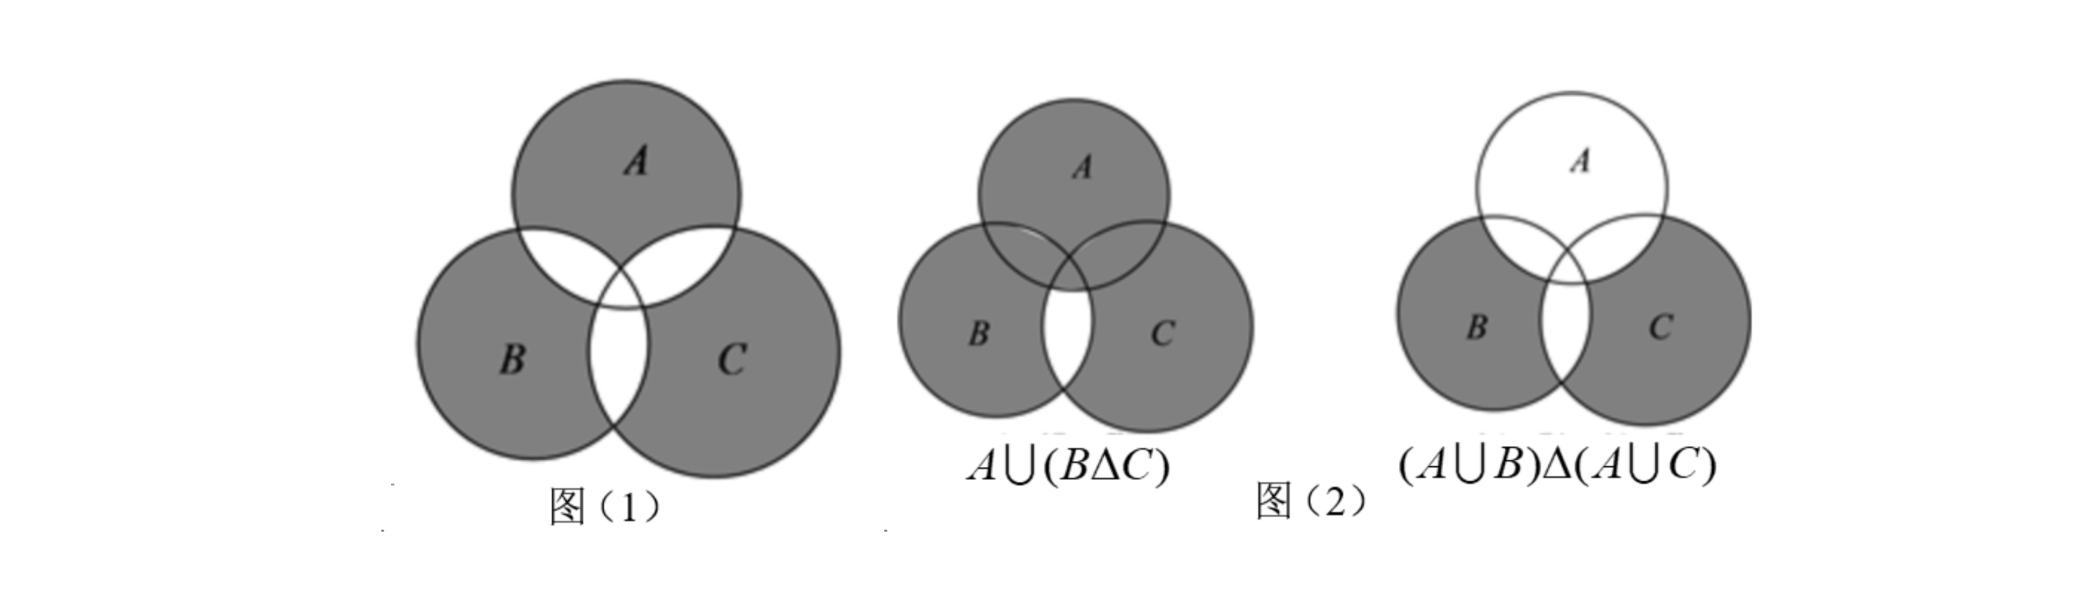
\includegraphics[width=0.92\textwidth]{figures/gao73_q16_symdiff.png}
\end{center}
\step{故选 $B$.}
\solend
\fi

\end{enumerate}

\bigsec{三、解答题}

\begin{enumerate}
\setcounter{enumi}{16}

\item （1）解不等式 $\dfrac{2-x}{x+3}>1$；

（2）已知 $a$ 是实数，试解关于 $x$ 的不等式：$x^2+(a-1)x-a\geqslant0$.

\ifanswer
\solbegin
\stepm{(1)}{$\dfrac{2-x}{x+3}-1=\dfrac{-2x-1}{x+3}>0$，则 $(2x+1)(x+3)<0$，得 $-3<x<-\dfrac12$，}
\step{所以不等式解集为 $\left(-3,-\dfrac12\right)$；}
\stepm{(2)}{$x^2+(a-1)x-a=(x+a)(x-1)\geqslant0$，}
% 原卷 (2) 题干为 ≥0，但解析按 ≤0 给出“两根之间”的解集，照录（见文件头“原卷笔误/存疑”②）
\step{当 $-a<1$，即 $a>-1$ 时，解集为 $(-a,1)$；}
\step{当 $-a=1$，即 $a=-1$ 时，解集为 $\R$；}
\step{当 $-a>1$，即 $a<-1$ 时，解集为 $(1,-a)$；}
\step{综上，当 $a>-1$ 时，解集为 $(-a,1)$；}
\step{当 $a=-1$ 时，解集为 $\R$；}
\step{当 $a<-1$ 时，解集为 $(1,-a)$.}
\solend
\fi

\ansspace[5]

\item （1）设 $a$、$b$ 是两个正数. 已知 $a>b$，比较 $\dfrac{2a+b}{a+2b}$ 与 $\dfrac ab$ 的值的大小；

（2）若实数 $a$ 满足 $\sqrt{(2023-a)^2}+\sqrt{a-2024}=a$，求 $a-2023^2$ 的值.

\ifanswer
\solbegin
\stepm{(1)}{$\dfrac{2a+b}{a+2b}-\dfrac ab=\dfrac{b^2-a^2}{b(a+2b)}<0$，所以 $\dfrac{2a+b}{a+2b}<\dfrac ab$.}
\stepm{(2)}{因为 $a-2024\geqslant0$，所以 $a\geqslant2024$，}
\step{所以 $\sqrt{(2023-a)^2}+\sqrt{a-2024}=a-2023+\sqrt{a-2024}$，}
\step{即 $a-2023+\sqrt{a-2024}=a$，即 $\sqrt{a-2024}=2023$，}
\step{所以 $a-2024=2023^2$，所以 $a-2023^2=2024$.}
\solend
\fi

\ansspace[5]

\item 已知 $m\in\R$，集合 $A=\{x\mid-1\leqslant x\leqslant3\}$，$B=\{x\mid m-3<x\leqslant m+2\}$.

（1）若“$x\in A$”是“$x\in B$”的充分不必要条件，求 $m$ 的取值范围；

（2）若 $A\cap B\neq\varnothing$，求 $m$ 的取值范围.

\ifanswer
\solbegin
\stepm{(1)}{因为“$x\in A$”是“$x\in B$”的充分不必要条件，所以 $A$ 是 $B$ 的真子集，}
\step{需满足 $\begin{cases}m-3<-1\\ m+2\geqslant3\end{cases}$，解得 $\begin{cases}m<2\\ m\geqslant1\end{cases}$，所以 $m$ 的取值范围是 $[1,2)$.}
\stepm{(2)}{因为 $A\cap B\neq\varnothing$，所以 $\begin{cases}m+2\geqslant-1\\ m-3<3\end{cases}$，解得 $\begin{cases}m\geqslant-3\\ m<6\end{cases}$，}
\step{所以 $m$ 的取值范围是 $[-3,6)$.}
\solend
\fi

\ansspace[6]

\item 已知集合 $A=\{x\mid x<-2\text{ 或 }x\geqslant3\}$，$U=\R$.

（1）若 $B=\{x\mid mx-1>0\}$，当 $B\subseteq A$ 时，求实数 $m$ 的取值范围；

（2）若 $B=\{x\mid2m-6\leqslant x\leqslant m+4\}$，当 $B\cap\overline A=\varnothing$ 时，求实数 $m$ 的取值范围.

\ifanswer
\solbegin
\stepm{(1)}{当 $m=0$ 时，$B=\varnothing$，符合题意，}
\step{当 $m>0$ 时，$B=\left\{x\mid x>\dfrac1m\right\}$，则 $\dfrac1m\geqslant3$，解得 $0<m\leqslant\dfrac13$，}
\step{当 $m<0$ 时，$B=\left\{x\mid x<\dfrac1m\right\}$，则 $\dfrac1m\leqslant-2$，解得 $-\dfrac12\leqslant m<0$，}
\step{综上所述，实数 $m$ 的取值范围 $\left[-\dfrac12,\dfrac13\right]$；}
\stepm{(2)}{由题意得 $B=\{x\mid2m-6\leqslant x\leqslant m+4\}$，$\overline A=\{x\mid-2\leqslant x<3\}$，且 $B\cap\overline A=\varnothing$，}
\step{当 $B=\varnothing$ 时，$2m-6>m+4$，解得 $m>10$，}
\step{当 $B\neq\varnothing$ 时，$\begin{cases}2m-6\leqslant m+4\\ m+4<-2\end{cases}$ 或 $\begin{cases}2m-6\leqslant m+4\\ 2m-6\geqslant3\end{cases}$，解得 $m<-6$ 或 $\dfrac92\leqslant m\leqslant10$，}
\step{综上所述，实数 $m$ 的取值范围为 $(-\infty,-6)\cup\left[\dfrac92,+\infty\right)$.}
\solend
\fi

\ansspace[7]

\item 关于实数大小关系的基本事实是解决等式或不等式问题的逻辑基础. 两个正数的大小关系是完全确定的，但通过运算就会产生非常奇妙的变化，基本不等式就是其中之一. 通过运算（代数变形）可以解决很多关于基本不等式的问题.

例如此题：正实数 $x$、$y$，满足 $x+y=1$，求 $\dfrac1x+\dfrac4y$ 的最小值. 求解本问题的方法很多，其中一种求解方法是：$\dfrac1x+\dfrac4y=(x+y)\left(\dfrac1x+\dfrac4y\right)=5+\dfrac yx+\dfrac{4x}{y}\geqslant5+2\sqrt{\dfrac yx\cdot\dfrac{4x}{y}}=9$，当且仅当 $\dfrac yx=\dfrac{4x}{y}$ 即 $y=2x$ 且 $x+y=1$ 时，即 $x=\dfrac13$，$y=\dfrac23$ 时等号成立.

这种解题方法叫作“$1$”的代换，利用上述求解方法解决下列问题：

（1）正数 $a$、$b$ 满足 $a+b=1$，求 $\dfrac1a+\dfrac2b$ 的最小值；

（2）已知 $a$、$b$、$c$ 均为正实数，且 $\dfrac1a+\dfrac1b+\dfrac1c=1$，求证：$a+b+c\geqslant9$；

（3）已知 $a$、$b$、$x$、$y$ 均为正实数，且 $\dfrac{x^2}{a^2}-\dfrac{y^2}{b^2}=1$，求证：$a^2-b^2\leqslant(x-y)^2$.

\ifanswer
\solbegin
\stepm{(1)}{正数 $a$、$b$ 满足 $a+b=1$，}
\step{$\dfrac1a+\dfrac2b=(a+b)\left(\dfrac1a+\dfrac2b\right)=1+2+\dfrac ba+\dfrac{2a}{b}\geqslant3+2\sqrt{\dfrac ba\cdot\dfrac{2a}{b}}=3+2\sqrt2$，}
\step{当且仅当 $\dfrac ba=\dfrac{2a}{b}$ 即 $b=\sqrt2\,a$ 且 $a+b=1$ 时，}
\step{即 $a=\sqrt2-1$，$b=2-\sqrt2$ 时取等号.}
\stepm{(2)}{$a+b+c=\left(\dfrac1a+\dfrac1b+\dfrac1c\right)(a+b+c)=3+\dfrac ba+\dfrac ab+\dfrac ca+\dfrac ac+\dfrac cb+\dfrac bc$}
\step{$\geqslant3+2\sqrt{\dfrac ba\cdot\dfrac ab}+2\sqrt{\dfrac ca\cdot\dfrac ac}+2\sqrt{\dfrac cb\cdot\dfrac bc}=9$，当且仅当 $a=b=c=3$ 时取等号，}
\step{故 $a+b+c\geqslant9$.}
\stepm{(3)}{$a^2-b^2=(a^2-b^2)\left(\dfrac{x^2}{a^2}-\dfrac{y^2}{b^2}\right)=x^2+y^2-\dfrac{b^2x^2}{a^2}-\dfrac{a^2y^2}{b^2}$}
\step{$=x^2+y^2-\left(\dfrac{b^2x^2}{a^2}+\dfrac{a^2y^2}{b^2}\right)\leqslant x^2+y^2-2\cdot\dfrac{bx}{a}\cdot\dfrac{ay}{b}=x^2+y^2-2xy$}
\step{$=(x-y)^2$，当且仅当 $\dfrac{bx}{a}=\dfrac{ay}{b}$ 且 $\dfrac{x^2}{a^2}-\dfrac{y^2}{b^2}=1$ 时，}
\step{即 $x=\dfrac{a^2}{\sqrt{a^2-b^2}}$，$y=\dfrac{b^2}{\sqrt{a^2-b^2}}$，$a>b$ 时取等号，故 $a^2-b^2\leqslant(x-y)^2$.}
\solend
\fi

\ansspace*[7]

\end{enumerate}

\end{document}
"
% 紧凑版：xelatex "\def\iscompact{1}% 高一73_徐汇中学_10月月考.tex
%   —— 高一上数学“2026-2027 年徐汇中学高一上 10 月月考”（讲评版）
% 试卷版：xelatex 高一73_徐汇中学_10月月考.tex
% 答案版：xelatex "\def\isanswer{1}\input{高一73_徐汇中学_10月月考.tex}"
% 紧凑版：xelatex "\def\iscompact{1}\input{高一73_徐汇中学_10月月考.tex}"
%
% 原始材料：微信公众号“魔都数学加油站”文章，连载“27学年高一73”；
% 原文标题“27学年高一73——2026-2027年上海市徐汇中学高一上10月月考”；
% 原文链接：https://mp.weixin.qq.com/s/Pkk9tFr4qHS9BR_BPxvk6A。
% 页面标注发布时间 2026-10-21 20:41（上海）。
% 正文为 10 张 PNG 页（`原图/高一73_徐汇中学_10月月考/01..10.png`）：
% 第 1、4、6、9、10 页为 2560×3620，其余 5 页为 4762×6735，均按页序读取。
% 10 页全为试卷正文页（卷首标题在第 1 页页顶，卷末第 21 题 (3) 解析止于第 10 页），
% 无封面页、目录页、二维码或宣传页。粉色斜排“魔都数学加油站”为卷面水印，未录入。
%
% 卷首标题：照卷面印作“2026-2027 年徐汇中学高一上 10 月月考”（黑体加粗一行）。
% 原卷年份区间用半角连字符，本稿按全稿惯例排 en dash；原卷无副标题。
%
% 篇幅与题号：原卷自第 3 题起编号（第 1、2 题不在本卷内）。填空题 3—12（10 题）、
% 选择题 13—16（4 题）、解答题 17—21（5 题），共 19 题。本稿沿用原节与原题号，
% 只改排为全稿统一的大节样式。
%
% 讲评版：原卷第 3、4 题只印【答案】（“没有实数根”“真”），本稿只给 \ans{}；
% 其余 17 题均印【解析】，用 \solbegin…\solend。四道选择题的作答括号原卷即留空，
% 答案写在解析末句“故选 A／D／A／B”，照录在解析内，不另提 \ans{}。
%
% 副标题：原卷未印副标题。本稿按“知识模块”口径标作“集合与常用逻辑用语、不等式”：
% 19 题中集合与常用逻辑用语 9 题（第 3、4、7、11、12、13、16、19、20 题），
% 不等式 10 题（第 5、6、8、9、10、14、15、17、18、21 题），两类均确有分量，故并标。
% 口径同 高一63、高一68—72。
%
% 与原卷的排版差异：
%   ① 原卷每题下直接印【答案】/【解析】，本稿按全稿惯例将答案与解析置于答案版；
%   ② 原卷未印副标题，本稿按“知识模块”口径补出；
%   ③ 原卷填空横线约四个字宽，本稿按全稿惯例统一排 \blankline[4.4em]；
%   ④ 原卷数集记号排斜体 $R$（第 3、8、9、10、12、17、19、20 题等），本稿按全稿惯例
%      改用 $\R$（同 高一68—72）；空集记号原卷作 $\varnothing$，照录；
%   ⑤ 原卷句末标点多为西文句点，第 15 题题干“整数解只有 $-2$”后为全角逗号，
%      均逐处照录；第 16 题解析的集合运算用 $\Delta$ 表示对称差，照原卷符号排；
%   ⑥ 第 17—21 题的子问原卷印作“（1）…（2）…”，本稿按 高一69—72 成例用行内
%      “（1）（2）（3）”段，解析中的子问标号用 \stepm{(1)}{…}；
%   ⑦ 每道解答题原卷未留作答空白，本稿按全稿惯例加 \ansspace（末题用 \ansspace*）；
%   ⑧ 选择题的作答括号原卷排半角“(    )”，本稿按全稿惯例排 \mbox{（\quad）}；
%      选项行排照原卷——第 13 题一行四条、第 14—16 题一行四条；
%   ⑨ 第 15 题题干的不等式组、第 14、19、20 题解析中的不等式组，原卷均排作“{”
%      连接的多行式，本稿按全稿惯例排 cases；
%   ⑩ 第 16 题解析末尾有三幅韦恩图（图（1）与图（2）的两幅）：原卷印在【解析】中，
%      题干无“如图”二字。本稿按原卷截图裁取（`figures/gao73_q16_symdiff.png`，
%      由第 6 页原图裁出、去除粉色水印后转灰度，未放大），放在答案版解析④之后。
%
% 原卷笔误/存疑（均照录未改，正文对应处另有 % 注）：
%   ① 第 3 题题干“设 $a$、$b\in\R$，则方程 $x^2+ax+a-1=0$ 至少有一个实根”中
%      $b$ 未在方程或后文出现，疑为衍字；原卷如此，照录未改。
%   ② 第 17 题 (2) 题干为 $x^2+(a-1)x-a\geqslant0$，但解析按 $\leqslant0$ 给出解集：
%      $a>-1$ 时写 $(-a,1)$、$a<-1$ 时写 $(1,-a)$，恰是“两根之间”的区间。
%      按题干 $\geqslant0$ 应为 $(-\infty,-a]\cup[1,+\infty)$ 与 $(-\infty,1]\cup[-a,+\infty)$；
%      原卷如此，照录未改。
%
% 行数核对：逐题数 \step/\stepm 条数与原卷【解析】印刷行数，17 题逐一相符，
% 合计 104 条 / 104 行（Q5：1；Q6：2；Q7：4；Q8：4；Q9：3；Q10：4；Q11：8；
% Q12：7；Q13：7；Q14：5；Q15：7；Q16：15；Q17：9；Q18：5；Q19：4；Q20：8；Q21：11）。
% 另第 3、4 题只印【答案】，各提 \ans{}，不计入 \step 账。
%
% 插图：第 16 题解析末的 3 幅韦恩图，见上⑩；全卷题干无其他配图。
%
\documentclass[a4paper,11pt]{article}
\usepackage{common}

\begin{document}

\examtitlest[3]{2026--2027 年徐汇中学高一上 10 月月考}{集合与常用逻辑用语、不等式}

\bigsec{一、填空题}

\begin{enumerate}
\setcounter{enumi}{2}

% 原卷题干“设 a、b∈R”中的 b 未在方程中出现，照录（见文件头“原卷笔误/存疑”①）
\item 如果用反证法证明命题“设 $a$、$b\in\R$，则方程 $x^2+ax+a-1=0$ 至少有一个实根”，那么首先假设方程 $x^2+ax+a-1=0$\blankline[4.4em].

\ifanswer
\ans{没有实数根}
\fi

\item 命题“若 $\dfrac1x>1$，则 $x<1$”是\blankline[4.4em]命题（填“真”，“假”）.

\ifanswer
\ans{真}
\fi

\item 对数 $\log_a(5-a)$ 中实数 $a$ 的取值范围是\blankline[4.4em].

\ifanswer
\solbegin
\step{由对数定义得 $\begin{cases}a>0\\ a\neq1\\ 5-a>0\end{cases}$，解得 $0<a<1$ 或 $1<a<5$.}
\solend
\fi

\item 关于 $x$ 的不等式 $ax^2-(a+1)x+1\leqslant0\,(a<0)$ 的解集为\blankline[4.4em].

\ifanswer
\solbegin
\step{原不等式即 $(ax-1)(x-1)\leqslant0$，因为 $a<0$，所以 $\left(x-\dfrac1a\right)(x-1)\geqslant0$.}
\step{又 $\dfrac1a<0<1$，所以 $x\leqslant\dfrac1a$ 或 $x\geqslant1$，故解集为 $\left(-\infty,\dfrac1a\right]\cup[1,+\infty)$.}
\solend
\fi

\item 若集合 $A=\{x\mid x^2-2kx+7k=0\}$ 有且仅有三个真子集，则 $k$ 的取值范围是\blankline[4.4em].

\ifanswer
\solbegin
\step{因为集合 $A$ 有且仅有三个真子集，则 $2^n-1=3$，解得 $n=2$，}
\step{所以一元二次方程 $x^2-2kx+7k=0$ 有两个不同的实数解，}
\step{则 $\Delta=4k^2-28k>0$，解得 $k<0$ 或 $k>7$，}
\step{故 $k$ 的取值范围是 $(-\infty,0)\cup(7,+\infty)$.}
\solend
\fi

\item 已知关于 $x$ 的不等式 $kx^2-4kx+k-6<0$ 对任意 $x\in\R$ 恒成立，则 $k$ 的取值范围是\blankline[4.4em].

\ifanswer
\solbegin
\step{关于 $x$ 的不等式 $kx^2-4kx+k-6<0$ 对任意 $x\in\R$ 恒成立，}
\step{当 $k=0$ 时，$kx^2-4kx+k-6=-6<0$ 恒成立，}
\step{当 $k\neq0$ 时，则 $\begin{cases}\Delta=16k^2-4k(k-6)<0\\ k<0\end{cases}$，解得 $-2<k<0$，}
\step{综上，$k$ 的取值范围为 $(-2,0]$.}
\solend
\fi

\item 设 $x\in\R$，方程 $|x-1|+|2x-1|=|3x-2|$ 的解集为\blankline[4.4em].

\ifanswer
\solbegin
\step{因为 $|x-1|+|2x-1|\geqslant|(x-1)+(2x-1)|=|3x-2|$，}
\step{当且仅当 $(x-1)(2x-1)\geqslant0$，解得 $x\leqslant\dfrac12$ 或 $x\geqslant1$，}
\step{故方程 $|x-1|+|2x-1|=|3x-2|$ 的解集为 $\left(-\infty,\dfrac12\right]\cup[1,+\infty)$.}
\solend
\fi

\item 已知 $a\in\R$，若关于 $x$ 的方程 $x^2+ax+a^2-8=0$ 有两个实根 $x_1$、$x_2$，且 $\dfrac1{x_1}+\dfrac1{x_2}=-\dfrac12$，则 $a$ 的值为\blankline[4.4em].

\ifanswer
\solbegin
\step{由题意得 $\Delta=a^2-4(a^2-8)=32-3a^2\geqslant0$，解得 $a^2\leqslant\dfrac{32}3$，}
\step{由韦达定理得 $x_1+x_2=-a$，$x_1x_2=a^2-8$，}
\step{则 $\dfrac1{x_1}+\dfrac1{x_2}=\dfrac{x_1+x_2}{x_1x_2}=\dfrac{-a}{a^2-8}=-\dfrac12$，即 $a^2-2a-8=(a-4)(a+2)=0$，}
\step{解得 $a=4$ 或 $a=-2$. 又 $a^2\leqslant\dfrac{32}3$，则 $a=-2$.}
\solend
\fi

\item 甲、乙两人解关于 $x$ 的不等式 $x^2+bx+c<0$，甲写错了 $b$，正确计算后得到的解为 $\{x\mid1<x<2\}$；乙写错了 $c$，正确计算后得到的解为 $\{x\mid-4<x<1\}$. 那么不等式 $\dfrac{bx+c}{x-2}<0$ 的解为\blankline[4.4em].

\ifanswer
\solbegin
\step{由 $x^2+bx+c<0$ 的解为 $\{x\mid1<x<2\}$，}
\step{则 $1$ 和 $2$ 是方程 $x^2+bx+c=0$ 的两个根，}
\step{甲写错了 $b$，但 $c$ 是正确的，所以 $c=1\times2=2$；}
\step{由 $x^2+bx+c<0$ 的解为 $\{x\mid-4<x<1\}$，}
\step{则 $-4$ 和 $1$ 是方程 $x^2+bx+c=0$ 的两个根，}
\step{乙写错了 $c$，但 $b$ 是正确的，所以 $-b=-4+1=-3$，即 $b=3$.}
\step{由 $\dfrac{bx+c}{x-2}<0$，得 $\dfrac{3x+2}{x-2}<0$，即 $(3x+2)(x-2)<0$，解得 $-\dfrac23<x<2$，}
\step{所以不等式 $\dfrac{bx+c}{x-2}<0$ 的解为 $\left\{x\mid-\dfrac23<x<2\right\}$.}
\solend
\fi

\item 设 $a,b,c\in\R$，$S=\{x\mid(x+a)(x^2+bx+c)=0,x\in\R\}$，$T=\{x\mid(ax+1)(cx^2+bx+1)=0,x\in\R\}$. 若 $|S|$、$|T|$ 分别为集合 $S$、$T$ 的元素个数，则 $|S|+|T|$ 的所有可能取值组成的集合为\blankline[4.4em].

\ifanswer
\solbegin
\step{$x\neq0$ 时，$(ax+1)(cx^2+bx+1)=x^3\left(\dfrac1x+a\right)\left(\dfrac1{x^2}+\dfrac bx+c\right)$，}
\step{故 $S$、$T$ 的非零元按倒数一一对应，设其个数均为 $k$；}
\step{$0\notin T$，且 $0\in S\Leftrightarrow ac=0$. 当 $ac=0$ 时 $k\in\{0,1,2\}$，}
\step{当 $ac\neq0$ 时 $x=-a\neq0$ 是 $S$ 的非零元，$k\in\{1,2,3\}$.}
\step{因此 $|S|+|T|$ 分别可取 $2k+1\in\{1,3,5\}$ 与 $2k\in\{2,4,6\}$.}
\step{依次取 $(a,b,c)=(0,0,0),(1,0,1),(0,-2,1),(1,-2,1),(0,0,-1),(1,-5,6)$，可分别实现 $1,2,3,4,5,6$，}
\step{则 $|S|+|T|$ 的所有可能取值组成的集合为 $\{1,2,3,4,5,6\}$.}
\solend
\fi

\end{enumerate}

\bigsec{二、选择题}

\begin{enumerate}
\setcounter{enumi}{12}

\item 如果 $a>b$，$c\neq0$，那么下列不等式成立的是\mbox{（\quad）}

\keepwithprev
A. $a-c>b-c$\qquad B. $c-a>c-b$\qquad C. $ac>bc$\qquad D. $\dfrac ac>\dfrac bc$

\ifanswer
\solbegin
\step{对于 $A$：$a-c-(b-c)=a-b>0$，即 $a-c>b-c$，故 $A$ 正确；}
\step{对于 $B$：$c-a-(c-b)=b-a<0$，即 $c-a<c-b$，故 $B$ 错误；}
\step{对于 $C$：$ac-bc=c(a-b)$，已知 $a-b>0$，}
\step{当 $c<0$ 时，$c(a-b)<0$，此时 $ac<bc$，故 $C$ 错误；}
\step{对于 $D$：$\dfrac ac-\dfrac bc=\dfrac1c(a-b)$，已知 $a-b>0$，}
\step{当 $c<0$ 时，$\dfrac1c(a-b)<0$，此时 $\dfrac ac<\dfrac bc$，故 $D$ 错误.}
\step{故选 $A$.}
\solend
\fi

\item 若不等式 $|x+1|\leqslant a$ 成立的一个充分不必要条件是 $-3\leqslant x\leqslant4$，则整数 $a$ 的最小值为\mbox{（\quad）}

\keepwithprev
A. $2$\qquad B. $3$\qquad C. $4$\qquad D. $5$

\ifanswer
\solbegin
\step{若 $a<0$，则 $|x+1|\leqslant a$ 无解；}
\step{若 $a\geqslant0$，由 $|x+1|\leqslant a$，得 $-1-a\leqslant x\leqslant-1+a$，}
\step{因为 $|x+1|\leqslant a$ 成立的一个充分不必要条件是 $-3\leqslant x\leqslant4$，}
\step{所以 $\begin{cases}-1-a\leqslant-3\\ -1+a\geqslant4\end{cases}$，等号不同时成立，解得 $a\geqslant5$，}
\step{故整数 $a$ 的最小值为 $5$. 故选 $D$.}
\solend
\fi

\item 若关于 $x$ 的不等式组 $\begin{cases}x^2-x-2>0\\ 2x^2+(5+2k)x+5k<0\end{cases}$ 的整数解只有 $-2$，则实数 $k$ 的取值范围为\mbox{（\quad）}

\keepwithprev
A. $[-3,2)$\qquad B. $[1,2]$\qquad C. $(1,2]$\qquad D. $(1,2)$

\ifanswer
\solbegin
\step{由 $x^2-x-2>0$，得 $x>2$ 或 $x<-1$，}
\step{由 $2x^2+(2k+5)x+5k<0$，得 $(2x+5)(x+k)<0$.}
\step{①若 $-k<-\dfrac52$，即 $k>\dfrac52$ 时，解得 $-k<x<-\dfrac52$，}
\step{此时原不等式的解集为 $\left(-k,-\dfrac52\right)$，不符合题意；}
\step{②若 $k=\dfrac52$ 时，解得 $x\in\varnothing$，显然不符合题意；}
\step{③若 $k<\dfrac52$ 时，解得 $-\dfrac52<x<-k$，则 $-2<-k\leqslant3$，即 $-3\leqslant k<2$.}
\step{综上，实数 $k$ 的取值范围 $[-3,2)$. 故选 $A$.}
\solend
\fi

\item 定义集合运算 $A-B=\{x\mid x\in A\text{ 且 }x\notin B\}$ 称为集合 $A$ 与集合 $B$ 的差集；定义集合运算 $A\Delta B=(A-B)\cup(B-A)$ 称为集合 $A$ 与集合 $B$ 的对称差，有以下 $4$ 个等式：

① $A\Delta B=B\Delta A$；

② $(A\Delta B)\Delta C=A\Delta(B\Delta C)$；

③ $A\cap(B\Delta C)=(A\cap B)\Delta(A\cap C)$；

④ $A\cup(B\Delta C)=(A\cup B)\Delta(A\cup C)$.

则 $4$ 个等式中恒成立的是\mbox{（\quad）}

\keepwithprev
A. ①②\qquad B. ①②③\qquad C. ①②④\qquad D. ①②③④

\ifanswer
\solbegin
\step{对于①，由 $B\Delta A=(B-A)\cup(A-B)=(A-B)\cup(B-A)=A\Delta B$，}
\step{所以①正确；}
\step{对于②，}
\step{由 $A-B=\{x\mid x\in A\text{ 且 }x\notin B\}=\{x\mid x\in A,x\notin(A\cap B)\}=A-(A\cap B)$，}
\step{同理可得 $B-A=B-(A\cap B)$，}
\step{则 $A\Delta B=(A-B)\cup(B-A)=(A\cup B)-(A\cap B)$，}
\step{所以 $(A\Delta B)\Delta C=(A\Delta B)\cup C-(A\Delta B)\cap C$，}
\step{所以表示的集合为图（1）中阴影部分所表示的集合，如图所示，}
\step{同理 $A\Delta(B\Delta C)=A\cup(B\Delta C)-A\cap(B\Delta C)$，}
\step{也表示图（1）中阴影部分所表示的集合，}
\step{所以 $(A\Delta B)\Delta C=A\Delta(B\Delta C)$，所以②正确；}
\step{对于③，由 $A\cap(B\Delta C)=A\cap(B\cup C-B\cap C)=A\cap(B\cup C)-A\cap(B\cap C)$}
\step{$=(A\cap B)\cup(A\cap C)-(A\cap B)\cap(A\cap C)=(A\cap B)\Delta(A\cap C)$，所以③正确；}
\step{对于④，如图（2）所示，$A\cup(B\Delta C)\neq(A\cup B)\Delta(A\cup C)$，所以④错误.}
\begin{center}
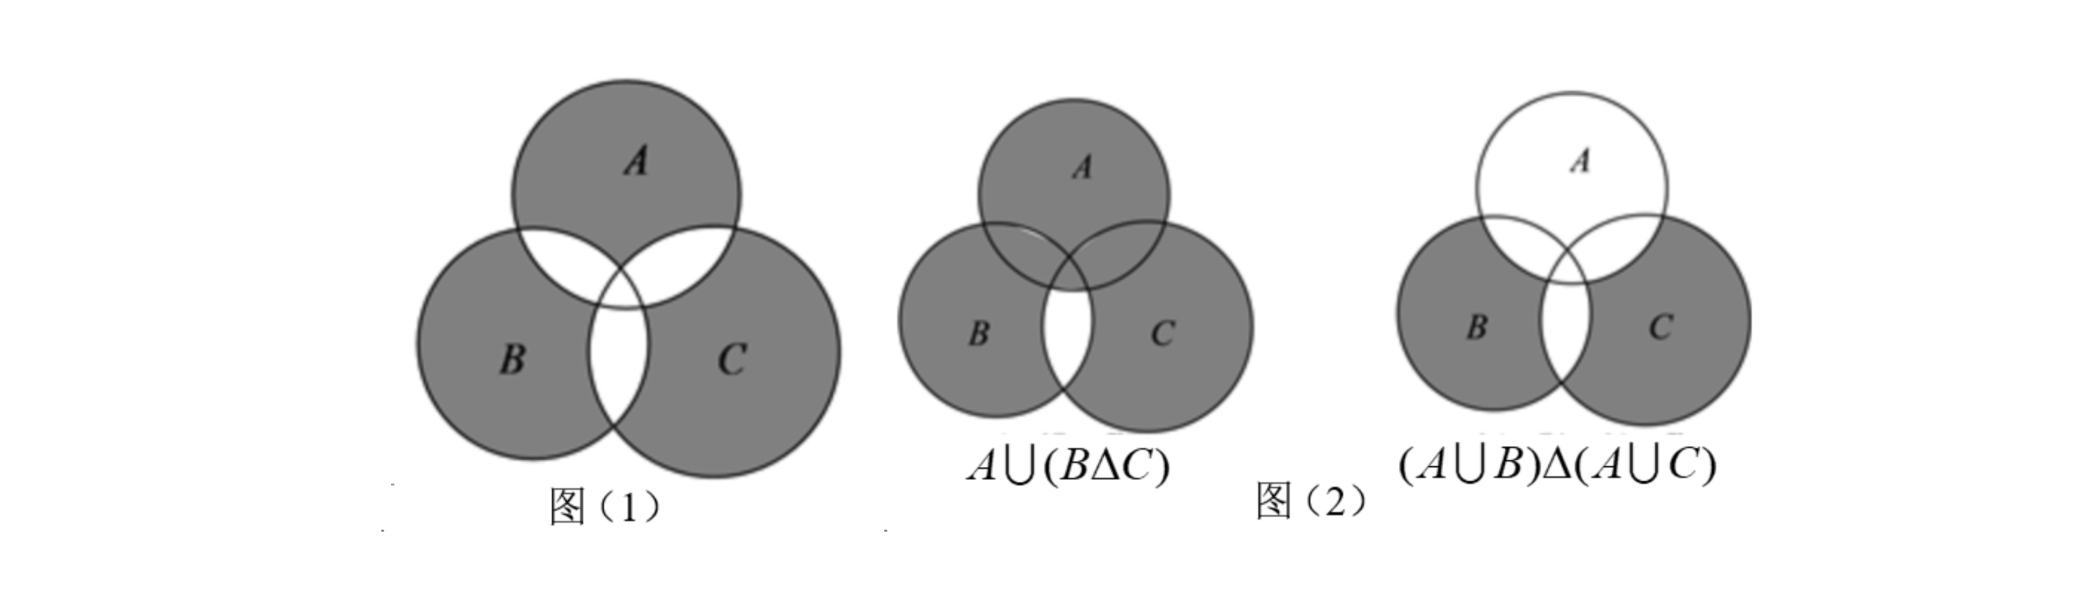
\includegraphics[width=0.92\textwidth]{figures/gao73_q16_symdiff.png}
\end{center}
\step{故选 $B$.}
\solend
\fi

\end{enumerate}

\bigsec{三、解答题}

\begin{enumerate}
\setcounter{enumi}{16}

\item （1）解不等式 $\dfrac{2-x}{x+3}>1$；

（2）已知 $a$ 是实数，试解关于 $x$ 的不等式：$x^2+(a-1)x-a\geqslant0$.

\ifanswer
\solbegin
\stepm{(1)}{$\dfrac{2-x}{x+3}-1=\dfrac{-2x-1}{x+3}>0$，则 $(2x+1)(x+3)<0$，得 $-3<x<-\dfrac12$，}
\step{所以不等式解集为 $\left(-3,-\dfrac12\right)$；}
\stepm{(2)}{$x^2+(a-1)x-a=(x+a)(x-1)\geqslant0$，}
% 原卷 (2) 题干为 ≥0，但解析按 ≤0 给出“两根之间”的解集，照录（见文件头“原卷笔误/存疑”②）
\step{当 $-a<1$，即 $a>-1$ 时，解集为 $(-a,1)$；}
\step{当 $-a=1$，即 $a=-1$ 时，解集为 $\R$；}
\step{当 $-a>1$，即 $a<-1$ 时，解集为 $(1,-a)$；}
\step{综上，当 $a>-1$ 时，解集为 $(-a,1)$；}
\step{当 $a=-1$ 时，解集为 $\R$；}
\step{当 $a<-1$ 时，解集为 $(1,-a)$.}
\solend
\fi

\ansspace[5]

\item （1）设 $a$、$b$ 是两个正数. 已知 $a>b$，比较 $\dfrac{2a+b}{a+2b}$ 与 $\dfrac ab$ 的值的大小；

（2）若实数 $a$ 满足 $\sqrt{(2023-a)^2}+\sqrt{a-2024}=a$，求 $a-2023^2$ 的值.

\ifanswer
\solbegin
\stepm{(1)}{$\dfrac{2a+b}{a+2b}-\dfrac ab=\dfrac{b^2-a^2}{b(a+2b)}<0$，所以 $\dfrac{2a+b}{a+2b}<\dfrac ab$.}
\stepm{(2)}{因为 $a-2024\geqslant0$，所以 $a\geqslant2024$，}
\step{所以 $\sqrt{(2023-a)^2}+\sqrt{a-2024}=a-2023+\sqrt{a-2024}$，}
\step{即 $a-2023+\sqrt{a-2024}=a$，即 $\sqrt{a-2024}=2023$，}
\step{所以 $a-2024=2023^2$，所以 $a-2023^2=2024$.}
\solend
\fi

\ansspace[5]

\item 已知 $m\in\R$，集合 $A=\{x\mid-1\leqslant x\leqslant3\}$，$B=\{x\mid m-3<x\leqslant m+2\}$.

（1）若“$x\in A$”是“$x\in B$”的充分不必要条件，求 $m$ 的取值范围；

（2）若 $A\cap B\neq\varnothing$，求 $m$ 的取值范围.

\ifanswer
\solbegin
\stepm{(1)}{因为“$x\in A$”是“$x\in B$”的充分不必要条件，所以 $A$ 是 $B$ 的真子集，}
\step{需满足 $\begin{cases}m-3<-1\\ m+2\geqslant3\end{cases}$，解得 $\begin{cases}m<2\\ m\geqslant1\end{cases}$，所以 $m$ 的取值范围是 $[1,2)$.}
\stepm{(2)}{因为 $A\cap B\neq\varnothing$，所以 $\begin{cases}m+2\geqslant-1\\ m-3<3\end{cases}$，解得 $\begin{cases}m\geqslant-3\\ m<6\end{cases}$，}
\step{所以 $m$ 的取值范围是 $[-3,6)$.}
\solend
\fi

\ansspace[6]

\item 已知集合 $A=\{x\mid x<-2\text{ 或 }x\geqslant3\}$，$U=\R$.

（1）若 $B=\{x\mid mx-1>0\}$，当 $B\subseteq A$ 时，求实数 $m$ 的取值范围；

（2）若 $B=\{x\mid2m-6\leqslant x\leqslant m+4\}$，当 $B\cap\overline A=\varnothing$ 时，求实数 $m$ 的取值范围.

\ifanswer
\solbegin
\stepm{(1)}{当 $m=0$ 时，$B=\varnothing$，符合题意，}
\step{当 $m>0$ 时，$B=\left\{x\mid x>\dfrac1m\right\}$，则 $\dfrac1m\geqslant3$，解得 $0<m\leqslant\dfrac13$，}
\step{当 $m<0$ 时，$B=\left\{x\mid x<\dfrac1m\right\}$，则 $\dfrac1m\leqslant-2$，解得 $-\dfrac12\leqslant m<0$，}
\step{综上所述，实数 $m$ 的取值范围 $\left[-\dfrac12,\dfrac13\right]$；}
\stepm{(2)}{由题意得 $B=\{x\mid2m-6\leqslant x\leqslant m+4\}$，$\overline A=\{x\mid-2\leqslant x<3\}$，且 $B\cap\overline A=\varnothing$，}
\step{当 $B=\varnothing$ 时，$2m-6>m+4$，解得 $m>10$，}
\step{当 $B\neq\varnothing$ 时，$\begin{cases}2m-6\leqslant m+4\\ m+4<-2\end{cases}$ 或 $\begin{cases}2m-6\leqslant m+4\\ 2m-6\geqslant3\end{cases}$，解得 $m<-6$ 或 $\dfrac92\leqslant m\leqslant10$，}
\step{综上所述，实数 $m$ 的取值范围为 $(-\infty,-6)\cup\left[\dfrac92,+\infty\right)$.}
\solend
\fi

\ansspace[7]

\item 关于实数大小关系的基本事实是解决等式或不等式问题的逻辑基础. 两个正数的大小关系是完全确定的，但通过运算就会产生非常奇妙的变化，基本不等式就是其中之一. 通过运算（代数变形）可以解决很多关于基本不等式的问题.

例如此题：正实数 $x$、$y$，满足 $x+y=1$，求 $\dfrac1x+\dfrac4y$ 的最小值. 求解本问题的方法很多，其中一种求解方法是：$\dfrac1x+\dfrac4y=(x+y)\left(\dfrac1x+\dfrac4y\right)=5+\dfrac yx+\dfrac{4x}{y}\geqslant5+2\sqrt{\dfrac yx\cdot\dfrac{4x}{y}}=9$，当且仅当 $\dfrac yx=\dfrac{4x}{y}$ 即 $y=2x$ 且 $x+y=1$ 时，即 $x=\dfrac13$，$y=\dfrac23$ 时等号成立.

这种解题方法叫作“$1$”的代换，利用上述求解方法解决下列问题：

（1）正数 $a$、$b$ 满足 $a+b=1$，求 $\dfrac1a+\dfrac2b$ 的最小值；

（2）已知 $a$、$b$、$c$ 均为正实数，且 $\dfrac1a+\dfrac1b+\dfrac1c=1$，求证：$a+b+c\geqslant9$；

（3）已知 $a$、$b$、$x$、$y$ 均为正实数，且 $\dfrac{x^2}{a^2}-\dfrac{y^2}{b^2}=1$，求证：$a^2-b^2\leqslant(x-y)^2$.

\ifanswer
\solbegin
\stepm{(1)}{正数 $a$、$b$ 满足 $a+b=1$，}
\step{$\dfrac1a+\dfrac2b=(a+b)\left(\dfrac1a+\dfrac2b\right)=1+2+\dfrac ba+\dfrac{2a}{b}\geqslant3+2\sqrt{\dfrac ba\cdot\dfrac{2a}{b}}=3+2\sqrt2$，}
\step{当且仅当 $\dfrac ba=\dfrac{2a}{b}$ 即 $b=\sqrt2\,a$ 且 $a+b=1$ 时，}
\step{即 $a=\sqrt2-1$，$b=2-\sqrt2$ 时取等号.}
\stepm{(2)}{$a+b+c=\left(\dfrac1a+\dfrac1b+\dfrac1c\right)(a+b+c)=3+\dfrac ba+\dfrac ab+\dfrac ca+\dfrac ac+\dfrac cb+\dfrac bc$}
\step{$\geqslant3+2\sqrt{\dfrac ba\cdot\dfrac ab}+2\sqrt{\dfrac ca\cdot\dfrac ac}+2\sqrt{\dfrac cb\cdot\dfrac bc}=9$，当且仅当 $a=b=c=3$ 时取等号，}
\step{故 $a+b+c\geqslant9$.}
\stepm{(3)}{$a^2-b^2=(a^2-b^2)\left(\dfrac{x^2}{a^2}-\dfrac{y^2}{b^2}\right)=x^2+y^2-\dfrac{b^2x^2}{a^2}-\dfrac{a^2y^2}{b^2}$}
\step{$=x^2+y^2-\left(\dfrac{b^2x^2}{a^2}+\dfrac{a^2y^2}{b^2}\right)\leqslant x^2+y^2-2\cdot\dfrac{bx}{a}\cdot\dfrac{ay}{b}=x^2+y^2-2xy$}
\step{$=(x-y)^2$，当且仅当 $\dfrac{bx}{a}=\dfrac{ay}{b}$ 且 $\dfrac{x^2}{a^2}-\dfrac{y^2}{b^2}=1$ 时，}
\step{即 $x=\dfrac{a^2}{\sqrt{a^2-b^2}}$，$y=\dfrac{b^2}{\sqrt{a^2-b^2}}$，$a>b$ 时取等号，故 $a^2-b^2\leqslant(x-y)^2$.}
\solend
\fi

\ansspace*[7]

\end{enumerate}

\end{document}
"
%
% 原始材料：微信公众号“魔都数学加油站”文章，连载“27学年高一73”；
% 原文标题“27学年高一73——2026-2027年上海市徐汇中学高一上10月月考”；
% 原文链接：https://mp.weixin.qq.com/s/Pkk9tFr4qHS9BR_BPxvk6A。
% 页面标注发布时间 2026-10-21 20:41（上海）。
% 正文为 10 张 PNG 页（`原图/高一73_徐汇中学_10月月考/01..10.png`）：
% 第 1、4、6、9、10 页为 2560×3620，其余 5 页为 4762×6735，均按页序读取。
% 10 页全为试卷正文页（卷首标题在第 1 页页顶，卷末第 21 题 (3) 解析止于第 10 页），
% 无封面页、目录页、二维码或宣传页。粉色斜排“魔都数学加油站”为卷面水印，未录入。
%
% 卷首标题：照卷面印作“2026-2027 年徐汇中学高一上 10 月月考”（黑体加粗一行）。
% 原卷年份区间用半角连字符，本稿按全稿惯例排 en dash；原卷无副标题。
%
% 篇幅与题号：原卷自第 3 题起编号（第 1、2 题不在本卷内）。填空题 3—12（10 题）、
% 选择题 13—16（4 题）、解答题 17—21（5 题），共 19 题。本稿沿用原节与原题号，
% 只改排为全稿统一的大节样式。
%
% 讲评版：原卷第 3、4 题只印【答案】（“没有实数根”“真”），本稿只给 \ans{}；
% 其余 17 题均印【解析】，用 \solbegin…\solend。四道选择题的作答括号原卷即留空，
% 答案写在解析末句“故选 A／D／A／B”，照录在解析内，不另提 \ans{}。
%
% 副标题：原卷未印副标题。本稿按“知识模块”口径标作“集合与常用逻辑用语、不等式”：
% 19 题中集合与常用逻辑用语 9 题（第 3、4、7、11、12、13、16、19、20 题），
% 不等式 10 题（第 5、6、8、9、10、14、15、17、18、21 题），两类均确有分量，故并标。
% 口径同 高一63、高一68—72。
%
% 与原卷的排版差异：
%   ① 原卷每题下直接印【答案】/【解析】，本稿按全稿惯例将答案与解析置于答案版；
%   ② 原卷未印副标题，本稿按“知识模块”口径补出；
%   ③ 原卷填空横线约四个字宽，本稿按全稿惯例统一排 \blankline[4.4em]；
%   ④ 原卷数集记号排斜体 $R$（第 3、8、9、10、12、17、19、20 题等），本稿按全稿惯例
%      改用 $\R$（同 高一68—72）；空集记号原卷作 $\varnothing$，照录；
%   ⑤ 原卷句末标点多为西文句点，第 15 题题干“整数解只有 $-2$”后为全角逗号，
%      均逐处照录；第 16 题解析的集合运算用 $\Delta$ 表示对称差，照原卷符号排；
%   ⑥ 第 17—21 题的子问原卷印作“（1）…（2）…”，本稿按 高一69—72 成例用行内
%      “（1）（2）（3）”段，解析中的子问标号用 \stepm{(1)}{…}；
%   ⑦ 每道解答题原卷未留作答空白，本稿按全稿惯例加 \ansspace（末题用 \ansspace*）；
%   ⑧ 选择题的作答括号原卷排半角“(    )”，本稿按全稿惯例排 \mbox{（\quad）}；
%      选项行排照原卷——第 13 题一行四条、第 14—16 题一行四条；
%   ⑨ 第 15 题题干的不等式组、第 14、19、20 题解析中的不等式组，原卷均排作“{”
%      连接的多行式，本稿按全稿惯例排 cases；
%   ⑩ 第 16 题解析末尾有三幅韦恩图（图（1）与图（2）的两幅）：原卷印在【解析】中，
%      题干无“如图”二字。本稿按原卷截图裁取（`figures/gao73_q16_symdiff.png`，
%      由第 6 页原图裁出、去除粉色水印后转灰度，未放大），放在答案版解析④之后。
%
% 原卷笔误/存疑（均照录未改，正文对应处另有 % 注）：
%   ① 第 3 题题干“设 $a$、$b\in\R$，则方程 $x^2+ax+a-1=0$ 至少有一个实根”中
%      $b$ 未在方程或后文出现，疑为衍字；原卷如此，照录未改。
%   ② 第 17 题 (2) 题干为 $x^2+(a-1)x-a\geqslant0$，但解析按 $\leqslant0$ 给出解集：
%      $a>-1$ 时写 $(-a,1)$、$a<-1$ 时写 $(1,-a)$，恰是“两根之间”的区间。
%      按题干 $\geqslant0$ 应为 $(-\infty,-a]\cup[1,+\infty)$ 与 $(-\infty,1]\cup[-a,+\infty)$；
%      原卷如此，照录未改。
%
% 行数核对：逐题数 \step/\stepm 条数与原卷【解析】印刷行数，17 题逐一相符，
% 合计 104 条 / 104 行（Q5：1；Q6：2；Q7：4；Q8：4；Q9：3；Q10：4；Q11：8；
% Q12：7；Q13：7；Q14：5；Q15：7；Q16：15；Q17：9；Q18：5；Q19：4；Q20：8；Q21：11）。
% 另第 3、4 题只印【答案】，各提 \ans{}，不计入 \step 账。
%
% 插图：第 16 题解析末的 3 幅韦恩图，见上⑩；全卷题干无其他配图。
%
\documentclass[a4paper,11pt]{article}
\usepackage{common}

\begin{document}

\examtitlest[3]{2026--2027 年徐汇中学高一上 10 月月考}{集合与常用逻辑用语、不等式}

\bigsec{一、填空题}

\begin{enumerate}
\setcounter{enumi}{2}

% 原卷题干“设 a、b∈R”中的 b 未在方程中出现，照录（见文件头“原卷笔误/存疑”①）
\item 如果用反证法证明命题“设 $a$、$b\in\R$，则方程 $x^2+ax+a-1=0$ 至少有一个实根”，那么首先假设方程 $x^2+ax+a-1=0$\blankline[4.4em].

\ifanswer
\ans{没有实数根}
\fi

\item 命题“若 $\dfrac1x>1$，则 $x<1$”是\blankline[4.4em]命题（填“真”，“假”）.

\ifanswer
\ans{真}
\fi

\item 对数 $\log_a(5-a)$ 中实数 $a$ 的取值范围是\blankline[4.4em].

\ifanswer
\solbegin
\step{由对数定义得 $\begin{cases}a>0\\ a\neq1\\ 5-a>0\end{cases}$，解得 $0<a<1$ 或 $1<a<5$.}
\solend
\fi

\item 关于 $x$ 的不等式 $ax^2-(a+1)x+1\leqslant0\,(a<0)$ 的解集为\blankline[4.4em].

\ifanswer
\solbegin
\step{原不等式即 $(ax-1)(x-1)\leqslant0$，因为 $a<0$，所以 $\left(x-\dfrac1a\right)(x-1)\geqslant0$.}
\step{又 $\dfrac1a<0<1$，所以 $x\leqslant\dfrac1a$ 或 $x\geqslant1$，故解集为 $\left(-\infty,\dfrac1a\right]\cup[1,+\infty)$.}
\solend
\fi

\item 若集合 $A=\{x\mid x^2-2kx+7k=0\}$ 有且仅有三个真子集，则 $k$ 的取值范围是\blankline[4.4em].

\ifanswer
\solbegin
\step{因为集合 $A$ 有且仅有三个真子集，则 $2^n-1=3$，解得 $n=2$，}
\step{所以一元二次方程 $x^2-2kx+7k=0$ 有两个不同的实数解，}
\step{则 $\Delta=4k^2-28k>0$，解得 $k<0$ 或 $k>7$，}
\step{故 $k$ 的取值范围是 $(-\infty,0)\cup(7,+\infty)$.}
\solend
\fi

\item 已知关于 $x$ 的不等式 $kx^2-4kx+k-6<0$ 对任意 $x\in\R$ 恒成立，则 $k$ 的取值范围是\blankline[4.4em].

\ifanswer
\solbegin
\step{关于 $x$ 的不等式 $kx^2-4kx+k-6<0$ 对任意 $x\in\R$ 恒成立，}
\step{当 $k=0$ 时，$kx^2-4kx+k-6=-6<0$ 恒成立，}
\step{当 $k\neq0$ 时，则 $\begin{cases}\Delta=16k^2-4k(k-6)<0\\ k<0\end{cases}$，解得 $-2<k<0$，}
\step{综上，$k$ 的取值范围为 $(-2,0]$.}
\solend
\fi

\item 设 $x\in\R$，方程 $|x-1|+|2x-1|=|3x-2|$ 的解集为\blankline[4.4em].

\ifanswer
\solbegin
\step{因为 $|x-1|+|2x-1|\geqslant|(x-1)+(2x-1)|=|3x-2|$，}
\step{当且仅当 $(x-1)(2x-1)\geqslant0$，解得 $x\leqslant\dfrac12$ 或 $x\geqslant1$，}
\step{故方程 $|x-1|+|2x-1|=|3x-2|$ 的解集为 $\left(-\infty,\dfrac12\right]\cup[1,+\infty)$.}
\solend
\fi

\item 已知 $a\in\R$，若关于 $x$ 的方程 $x^2+ax+a^2-8=0$ 有两个实根 $x_1$、$x_2$，且 $\dfrac1{x_1}+\dfrac1{x_2}=-\dfrac12$，则 $a$ 的值为\blankline[4.4em].

\ifanswer
\solbegin
\step{由题意得 $\Delta=a^2-4(a^2-8)=32-3a^2\geqslant0$，解得 $a^2\leqslant\dfrac{32}3$，}
\step{由韦达定理得 $x_1+x_2=-a$，$x_1x_2=a^2-8$，}
\step{则 $\dfrac1{x_1}+\dfrac1{x_2}=\dfrac{x_1+x_2}{x_1x_2}=\dfrac{-a}{a^2-8}=-\dfrac12$，即 $a^2-2a-8=(a-4)(a+2)=0$，}
\step{解得 $a=4$ 或 $a=-2$. 又 $a^2\leqslant\dfrac{32}3$，则 $a=-2$.}
\solend
\fi

\item 甲、乙两人解关于 $x$ 的不等式 $x^2+bx+c<0$，甲写错了 $b$，正确计算后得到的解为 $\{x\mid1<x<2\}$；乙写错了 $c$，正确计算后得到的解为 $\{x\mid-4<x<1\}$. 那么不等式 $\dfrac{bx+c}{x-2}<0$ 的解为\blankline[4.4em].

\ifanswer
\solbegin
\step{由 $x^2+bx+c<0$ 的解为 $\{x\mid1<x<2\}$，}
\step{则 $1$ 和 $2$ 是方程 $x^2+bx+c=0$ 的两个根，}
\step{甲写错了 $b$，但 $c$ 是正确的，所以 $c=1\times2=2$；}
\step{由 $x^2+bx+c<0$ 的解为 $\{x\mid-4<x<1\}$，}
\step{则 $-4$ 和 $1$ 是方程 $x^2+bx+c=0$ 的两个根，}
\step{乙写错了 $c$，但 $b$ 是正确的，所以 $-b=-4+1=-3$，即 $b=3$.}
\step{由 $\dfrac{bx+c}{x-2}<0$，得 $\dfrac{3x+2}{x-2}<0$，即 $(3x+2)(x-2)<0$，解得 $-\dfrac23<x<2$，}
\step{所以不等式 $\dfrac{bx+c}{x-2}<0$ 的解为 $\left\{x\mid-\dfrac23<x<2\right\}$.}
\solend
\fi

\item 设 $a,b,c\in\R$，$S=\{x\mid(x+a)(x^2+bx+c)=0,x\in\R\}$，$T=\{x\mid(ax+1)(cx^2+bx+1)=0,x\in\R\}$. 若 $|S|$、$|T|$ 分别为集合 $S$、$T$ 的元素个数，则 $|S|+|T|$ 的所有可能取值组成的集合为\blankline[4.4em].

\ifanswer
\solbegin
\step{$x\neq0$ 时，$(ax+1)(cx^2+bx+1)=x^3\left(\dfrac1x+a\right)\left(\dfrac1{x^2}+\dfrac bx+c\right)$，}
\step{故 $S$、$T$ 的非零元按倒数一一对应，设其个数均为 $k$；}
\step{$0\notin T$，且 $0\in S\Leftrightarrow ac=0$. 当 $ac=0$ 时 $k\in\{0,1,2\}$，}
\step{当 $ac\neq0$ 时 $x=-a\neq0$ 是 $S$ 的非零元，$k\in\{1,2,3\}$.}
\step{因此 $|S|+|T|$ 分别可取 $2k+1\in\{1,3,5\}$ 与 $2k\in\{2,4,6\}$.}
\step{依次取 $(a,b,c)=(0,0,0),(1,0,1),(0,-2,1),(1,-2,1),(0,0,-1),(1,-5,6)$，可分别实现 $1,2,3,4,5,6$，}
\step{则 $|S|+|T|$ 的所有可能取值组成的集合为 $\{1,2,3,4,5,6\}$.}
\solend
\fi

\end{enumerate}

\bigsec{二、选择题}

\begin{enumerate}
\setcounter{enumi}{12}

\item 如果 $a>b$，$c\neq0$，那么下列不等式成立的是\mbox{（\quad）}

\keepwithprev
A. $a-c>b-c$\qquad B. $c-a>c-b$\qquad C. $ac>bc$\qquad D. $\dfrac ac>\dfrac bc$

\ifanswer
\solbegin
\step{对于 $A$：$a-c-(b-c)=a-b>0$，即 $a-c>b-c$，故 $A$ 正确；}
\step{对于 $B$：$c-a-(c-b)=b-a<0$，即 $c-a<c-b$，故 $B$ 错误；}
\step{对于 $C$：$ac-bc=c(a-b)$，已知 $a-b>0$，}
\step{当 $c<0$ 时，$c(a-b)<0$，此时 $ac<bc$，故 $C$ 错误；}
\step{对于 $D$：$\dfrac ac-\dfrac bc=\dfrac1c(a-b)$，已知 $a-b>0$，}
\step{当 $c<0$ 时，$\dfrac1c(a-b)<0$，此时 $\dfrac ac<\dfrac bc$，故 $D$ 错误.}
\step{故选 $A$.}
\solend
\fi

\item 若不等式 $|x+1|\leqslant a$ 成立的一个充分不必要条件是 $-3\leqslant x\leqslant4$，则整数 $a$ 的最小值为\mbox{（\quad）}

\keepwithprev
A. $2$\qquad B. $3$\qquad C. $4$\qquad D. $5$

\ifanswer
\solbegin
\step{若 $a<0$，则 $|x+1|\leqslant a$ 无解；}
\step{若 $a\geqslant0$，由 $|x+1|\leqslant a$，得 $-1-a\leqslant x\leqslant-1+a$，}
\step{因为 $|x+1|\leqslant a$ 成立的一个充分不必要条件是 $-3\leqslant x\leqslant4$，}
\step{所以 $\begin{cases}-1-a\leqslant-3\\ -1+a\geqslant4\end{cases}$，等号不同时成立，解得 $a\geqslant5$，}
\step{故整数 $a$ 的最小值为 $5$. 故选 $D$.}
\solend
\fi

\item 若关于 $x$ 的不等式组 $\begin{cases}x^2-x-2>0\\ 2x^2+(5+2k)x+5k<0\end{cases}$ 的整数解只有 $-2$，则实数 $k$ 的取值范围为\mbox{（\quad）}

\keepwithprev
A. $[-3,2)$\qquad B. $[1,2]$\qquad C. $(1,2]$\qquad D. $(1,2)$

\ifanswer
\solbegin
\step{由 $x^2-x-2>0$，得 $x>2$ 或 $x<-1$，}
\step{由 $2x^2+(2k+5)x+5k<0$，得 $(2x+5)(x+k)<0$.}
\step{①若 $-k<-\dfrac52$，即 $k>\dfrac52$ 时，解得 $-k<x<-\dfrac52$，}
\step{此时原不等式的解集为 $\left(-k,-\dfrac52\right)$，不符合题意；}
\step{②若 $k=\dfrac52$ 时，解得 $x\in\varnothing$，显然不符合题意；}
\step{③若 $k<\dfrac52$ 时，解得 $-\dfrac52<x<-k$，则 $-2<-k\leqslant3$，即 $-3\leqslant k<2$.}
\step{综上，实数 $k$ 的取值范围 $[-3,2)$. 故选 $A$.}
\solend
\fi

\item 定义集合运算 $A-B=\{x\mid x\in A\text{ 且 }x\notin B\}$ 称为集合 $A$ 与集合 $B$ 的差集；定义集合运算 $A\Delta B=(A-B)\cup(B-A)$ 称为集合 $A$ 与集合 $B$ 的对称差，有以下 $4$ 个等式：

① $A\Delta B=B\Delta A$；

② $(A\Delta B)\Delta C=A\Delta(B\Delta C)$；

③ $A\cap(B\Delta C)=(A\cap B)\Delta(A\cap C)$；

④ $A\cup(B\Delta C)=(A\cup B)\Delta(A\cup C)$.

则 $4$ 个等式中恒成立的是\mbox{（\quad）}

\keepwithprev
A. ①②\qquad B. ①②③\qquad C. ①②④\qquad D. ①②③④

\ifanswer
\solbegin
\step{对于①，由 $B\Delta A=(B-A)\cup(A-B)=(A-B)\cup(B-A)=A\Delta B$，}
\step{所以①正确；}
\step{对于②，}
\step{由 $A-B=\{x\mid x\in A\text{ 且 }x\notin B\}=\{x\mid x\in A,x\notin(A\cap B)\}=A-(A\cap B)$，}
\step{同理可得 $B-A=B-(A\cap B)$，}
\step{则 $A\Delta B=(A-B)\cup(B-A)=(A\cup B)-(A\cap B)$，}
\step{所以 $(A\Delta B)\Delta C=(A\Delta B)\cup C-(A\Delta B)\cap C$，}
\step{所以表示的集合为图（1）中阴影部分所表示的集合，如图所示，}
\step{同理 $A\Delta(B\Delta C)=A\cup(B\Delta C)-A\cap(B\Delta C)$，}
\step{也表示图（1）中阴影部分所表示的集合，}
\step{所以 $(A\Delta B)\Delta C=A\Delta(B\Delta C)$，所以②正确；}
\step{对于③，由 $A\cap(B\Delta C)=A\cap(B\cup C-B\cap C)=A\cap(B\cup C)-A\cap(B\cap C)$}
\step{$=(A\cap B)\cup(A\cap C)-(A\cap B)\cap(A\cap C)=(A\cap B)\Delta(A\cap C)$，所以③正确；}
\step{对于④，如图（2）所示，$A\cup(B\Delta C)\neq(A\cup B)\Delta(A\cup C)$，所以④错误.}
\begin{center}
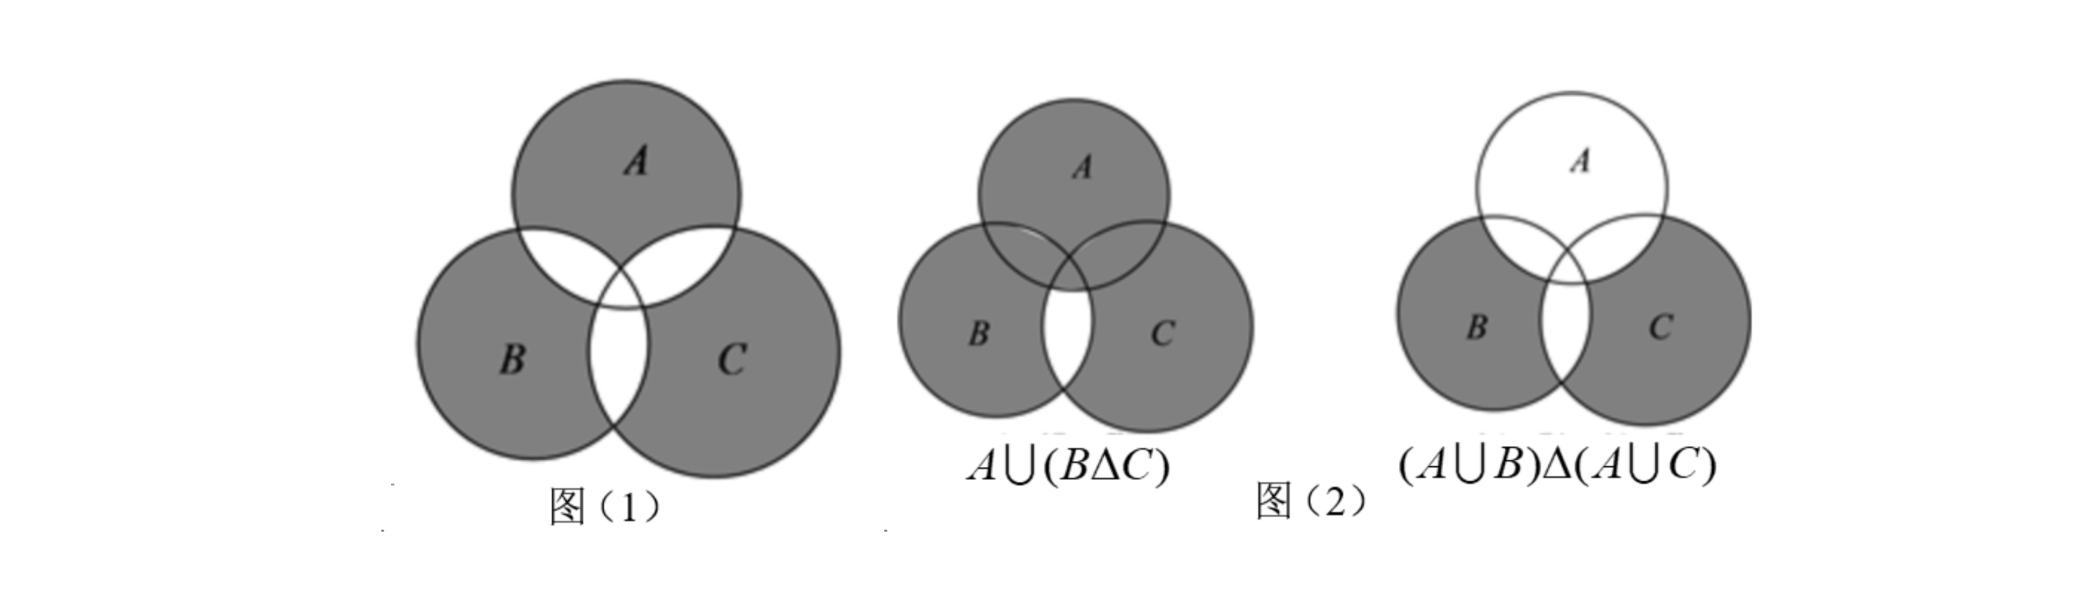
\includegraphics[width=0.92\textwidth]{figures/gao73_q16_symdiff.png}
\end{center}
\step{故选 $B$.}
\solend
\fi

\end{enumerate}

\bigsec{三、解答题}

\begin{enumerate}
\setcounter{enumi}{16}

\item （1）解不等式 $\dfrac{2-x}{x+3}>1$；

（2）已知 $a$ 是实数，试解关于 $x$ 的不等式：$x^2+(a-1)x-a\geqslant0$.

\ifanswer
\solbegin
\stepm{(1)}{$\dfrac{2-x}{x+3}-1=\dfrac{-2x-1}{x+3}>0$，则 $(2x+1)(x+3)<0$，得 $-3<x<-\dfrac12$，}
\step{所以不等式解集为 $\left(-3,-\dfrac12\right)$；}
\stepm{(2)}{$x^2+(a-1)x-a=(x+a)(x-1)\geqslant0$，}
% 原卷 (2) 题干为 ≥0，但解析按 ≤0 给出“两根之间”的解集，照录（见文件头“原卷笔误/存疑”②）
\step{当 $-a<1$，即 $a>-1$ 时，解集为 $(-a,1)$；}
\step{当 $-a=1$，即 $a=-1$ 时，解集为 $\R$；}
\step{当 $-a>1$，即 $a<-1$ 时，解集为 $(1,-a)$；}
\step{综上，当 $a>-1$ 时，解集为 $(-a,1)$；}
\step{当 $a=-1$ 时，解集为 $\R$；}
\step{当 $a<-1$ 时，解集为 $(1,-a)$.}
\solend
\fi

\ansspace[5]

\item （1）设 $a$、$b$ 是两个正数. 已知 $a>b$，比较 $\dfrac{2a+b}{a+2b}$ 与 $\dfrac ab$ 的值的大小；

（2）若实数 $a$ 满足 $\sqrt{(2023-a)^2}+\sqrt{a-2024}=a$，求 $a-2023^2$ 的值.

\ifanswer
\solbegin
\stepm{(1)}{$\dfrac{2a+b}{a+2b}-\dfrac ab=\dfrac{b^2-a^2}{b(a+2b)}<0$，所以 $\dfrac{2a+b}{a+2b}<\dfrac ab$.}
\stepm{(2)}{因为 $a-2024\geqslant0$，所以 $a\geqslant2024$，}
\step{所以 $\sqrt{(2023-a)^2}+\sqrt{a-2024}=a-2023+\sqrt{a-2024}$，}
\step{即 $a-2023+\sqrt{a-2024}=a$，即 $\sqrt{a-2024}=2023$，}
\step{所以 $a-2024=2023^2$，所以 $a-2023^2=2024$.}
\solend
\fi

\ansspace[5]

\item 已知 $m\in\R$，集合 $A=\{x\mid-1\leqslant x\leqslant3\}$，$B=\{x\mid m-3<x\leqslant m+2\}$.

（1）若“$x\in A$”是“$x\in B$”的充分不必要条件，求 $m$ 的取值范围；

（2）若 $A\cap B\neq\varnothing$，求 $m$ 的取值范围.

\ifanswer
\solbegin
\stepm{(1)}{因为“$x\in A$”是“$x\in B$”的充分不必要条件，所以 $A$ 是 $B$ 的真子集，}
\step{需满足 $\begin{cases}m-3<-1\\ m+2\geqslant3\end{cases}$，解得 $\begin{cases}m<2\\ m\geqslant1\end{cases}$，所以 $m$ 的取值范围是 $[1,2)$.}
\stepm{(2)}{因为 $A\cap B\neq\varnothing$，所以 $\begin{cases}m+2\geqslant-1\\ m-3<3\end{cases}$，解得 $\begin{cases}m\geqslant-3\\ m<6\end{cases}$，}
\step{所以 $m$ 的取值范围是 $[-3,6)$.}
\solend
\fi

\ansspace[6]

\item 已知集合 $A=\{x\mid x<-2\text{ 或 }x\geqslant3\}$，$U=\R$.

（1）若 $B=\{x\mid mx-1>0\}$，当 $B\subseteq A$ 时，求实数 $m$ 的取值范围；

（2）若 $B=\{x\mid2m-6\leqslant x\leqslant m+4\}$，当 $B\cap\overline A=\varnothing$ 时，求实数 $m$ 的取值范围.

\ifanswer
\solbegin
\stepm{(1)}{当 $m=0$ 时，$B=\varnothing$，符合题意，}
\step{当 $m>0$ 时，$B=\left\{x\mid x>\dfrac1m\right\}$，则 $\dfrac1m\geqslant3$，解得 $0<m\leqslant\dfrac13$，}
\step{当 $m<0$ 时，$B=\left\{x\mid x<\dfrac1m\right\}$，则 $\dfrac1m\leqslant-2$，解得 $-\dfrac12\leqslant m<0$，}
\step{综上所述，实数 $m$ 的取值范围 $\left[-\dfrac12,\dfrac13\right]$；}
\stepm{(2)}{由题意得 $B=\{x\mid2m-6\leqslant x\leqslant m+4\}$，$\overline A=\{x\mid-2\leqslant x<3\}$，且 $B\cap\overline A=\varnothing$，}
\step{当 $B=\varnothing$ 时，$2m-6>m+4$，解得 $m>10$，}
\step{当 $B\neq\varnothing$ 时，$\begin{cases}2m-6\leqslant m+4\\ m+4<-2\end{cases}$ 或 $\begin{cases}2m-6\leqslant m+4\\ 2m-6\geqslant3\end{cases}$，解得 $m<-6$ 或 $\dfrac92\leqslant m\leqslant10$，}
\step{综上所述，实数 $m$ 的取值范围为 $(-\infty,-6)\cup\left[\dfrac92,+\infty\right)$.}
\solend
\fi

\ansspace[7]

\item 关于实数大小关系的基本事实是解决等式或不等式问题的逻辑基础. 两个正数的大小关系是完全确定的，但通过运算就会产生非常奇妙的变化，基本不等式就是其中之一. 通过运算（代数变形）可以解决很多关于基本不等式的问题.

例如此题：正实数 $x$、$y$，满足 $x+y=1$，求 $\dfrac1x+\dfrac4y$ 的最小值. 求解本问题的方法很多，其中一种求解方法是：$\dfrac1x+\dfrac4y=(x+y)\left(\dfrac1x+\dfrac4y\right)=5+\dfrac yx+\dfrac{4x}{y}\geqslant5+2\sqrt{\dfrac yx\cdot\dfrac{4x}{y}}=9$，当且仅当 $\dfrac yx=\dfrac{4x}{y}$ 即 $y=2x$ 且 $x+y=1$ 时，即 $x=\dfrac13$，$y=\dfrac23$ 时等号成立.

这种解题方法叫作“$1$”的代换，利用上述求解方法解决下列问题：

（1）正数 $a$、$b$ 满足 $a+b=1$，求 $\dfrac1a+\dfrac2b$ 的最小值；

（2）已知 $a$、$b$、$c$ 均为正实数，且 $\dfrac1a+\dfrac1b+\dfrac1c=1$，求证：$a+b+c\geqslant9$；

（3）已知 $a$、$b$、$x$、$y$ 均为正实数，且 $\dfrac{x^2}{a^2}-\dfrac{y^2}{b^2}=1$，求证：$a^2-b^2\leqslant(x-y)^2$.

\ifanswer
\solbegin
\stepm{(1)}{正数 $a$、$b$ 满足 $a+b=1$，}
\step{$\dfrac1a+\dfrac2b=(a+b)\left(\dfrac1a+\dfrac2b\right)=1+2+\dfrac ba+\dfrac{2a}{b}\geqslant3+2\sqrt{\dfrac ba\cdot\dfrac{2a}{b}}=3+2\sqrt2$，}
\step{当且仅当 $\dfrac ba=\dfrac{2a}{b}$ 即 $b=\sqrt2\,a$ 且 $a+b=1$ 时，}
\step{即 $a=\sqrt2-1$，$b=2-\sqrt2$ 时取等号.}
\stepm{(2)}{$a+b+c=\left(\dfrac1a+\dfrac1b+\dfrac1c\right)(a+b+c)=3+\dfrac ba+\dfrac ab+\dfrac ca+\dfrac ac+\dfrac cb+\dfrac bc$}
\step{$\geqslant3+2\sqrt{\dfrac ba\cdot\dfrac ab}+2\sqrt{\dfrac ca\cdot\dfrac ac}+2\sqrt{\dfrac cb\cdot\dfrac bc}=9$，当且仅当 $a=b=c=3$ 时取等号，}
\step{故 $a+b+c\geqslant9$.}
\stepm{(3)}{$a^2-b^2=(a^2-b^2)\left(\dfrac{x^2}{a^2}-\dfrac{y^2}{b^2}\right)=x^2+y^2-\dfrac{b^2x^2}{a^2}-\dfrac{a^2y^2}{b^2}$}
\step{$=x^2+y^2-\left(\dfrac{b^2x^2}{a^2}+\dfrac{a^2y^2}{b^2}\right)\leqslant x^2+y^2-2\cdot\dfrac{bx}{a}\cdot\dfrac{ay}{b}=x^2+y^2-2xy$}
\step{$=(x-y)^2$，当且仅当 $\dfrac{bx}{a}=\dfrac{ay}{b}$ 且 $\dfrac{x^2}{a^2}-\dfrac{y^2}{b^2}=1$ 时，}
\step{即 $x=\dfrac{a^2}{\sqrt{a^2-b^2}}$，$y=\dfrac{b^2}{\sqrt{a^2-b^2}}$，$a>b$ 时取等号，故 $a^2-b^2\leqslant(x-y)^2$.}
\solend
\fi

\ansspace*[7]

\end{enumerate}

\end{document}
"
%
% 原始材料：微信公众号“魔都数学加油站”文章，连载“27学年高一73”；
% 原文标题“27学年高一73——2026-2027年上海市徐汇中学高一上10月月考”；
% 原文链接：https://mp.weixin.qq.com/s/Pkk9tFr4qHS9BR_BPxvk6A。
% 页面标注发布时间 2026-10-21 20:41（上海）。
% 正文为 10 张 PNG 页（`原图/高一73_徐汇中学_10月月考/01..10.png`）：
% 第 1、4、6、9、10 页为 2560×3620，其余 5 页为 4762×6735，均按页序读取。
% 10 页全为试卷正文页（卷首标题在第 1 页页顶，卷末第 21 题 (3) 解析止于第 10 页），
% 无封面页、目录页、二维码或宣传页。粉色斜排“魔都数学加油站”为卷面水印，未录入。
%
% 卷首标题：照卷面印作“2026-2027 年徐汇中学高一上 10 月月考”（黑体加粗一行）。
% 原卷年份区间用半角连字符，本稿按全稿惯例排 en dash；原卷无副标题。
%
% 篇幅与题号：原卷自第 3 题起编号（第 1、2 题不在本卷内）。填空题 3—12（10 题）、
% 选择题 13—16（4 题）、解答题 17—21（5 题），共 19 题。本稿沿用原节与原题号，
% 只改排为全稿统一的大节样式。
%
% 讲评版：原卷第 3、4 题只印【答案】（“没有实数根”“真”），本稿只给 \ans{}；
% 其余 17 题均印【解析】，用 \solbegin…\solend。四道选择题的作答括号原卷即留空，
% 答案写在解析末句“故选 A／D／A／B”，照录在解析内，不另提 \ans{}。
%
% 副标题：原卷未印副标题。本稿按“知识模块”口径标作“集合与常用逻辑用语、不等式”：
% 19 题中集合与常用逻辑用语 9 题（第 3、4、7、11、12、13、16、19、20 题），
% 不等式 10 题（第 5、6、8、9、10、14、15、17、18、21 题），两类均确有分量，故并标。
% 口径同 高一63、高一68—72。
%
% 与原卷的排版差异：
%   ① 原卷每题下直接印【答案】/【解析】，本稿按全稿惯例将答案与解析置于答案版；
%   ② 原卷未印副标题，本稿按“知识模块”口径补出；
%   ③ 原卷填空横线约四个字宽，本稿按全稿惯例统一排 \blankline[4.4em]；
%   ④ 原卷数集记号排斜体 $R$（第 3、8、9、10、12、17、19、20 题等），本稿按全稿惯例
%      改用 $\R$（同 高一68—72）；空集记号原卷作 $\varnothing$，照录；
%   ⑤ 原卷句末标点多为西文句点，第 15 题题干“整数解只有 $-2$”后为全角逗号，
%      均逐处照录；第 16 题解析的集合运算用 $\Delta$ 表示对称差，照原卷符号排；
%   ⑥ 第 17—21 题的子问原卷印作“（1）…（2）…”，本稿按 高一69—72 成例用行内
%      “（1）（2）（3）”段，解析中的子问标号用 \stepm{(1)}{…}；
%   ⑦ 每道解答题原卷未留作答空白，本稿按全稿惯例加 \ansspace（末题用 \ansspace*）；
%   ⑧ 选择题的作答括号原卷排半角“(    )”，本稿按全稿惯例排 \mbox{（\quad）}；
%      选项行排照原卷——第 13 题一行四条、第 14—16 题一行四条；
%   ⑨ 第 15 题题干的不等式组、第 14、19、20 题解析中的不等式组，原卷均排作“{”
%      连接的多行式，本稿按全稿惯例排 cases；
%   ⑩ 第 16 题解析末尾有三幅韦恩图（图（1）与图（2）的两幅）：原卷印在【解析】中，
%      题干无“如图”二字。本稿按原卷截图裁取（`figures/gao73_q16_symdiff.png`，
%      由第 6 页原图裁出、去除粉色水印后转灰度，未放大），放在答案版解析④之后。
%
% 原卷笔误/存疑（均照录未改，正文对应处另有 % 注）：
%   ① 第 3 题题干“设 $a$、$b\in\R$，则方程 $x^2+ax+a-1=0$ 至少有一个实根”中
%      $b$ 未在方程或后文出现，疑为衍字；原卷如此，照录未改。
%   ② 第 17 题 (2) 题干为 $x^2+(a-1)x-a\geqslant0$，但解析按 $\leqslant0$ 给出解集：
%      $a>-1$ 时写 $(-a,1)$、$a<-1$ 时写 $(1,-a)$，恰是“两根之间”的区间。
%      按题干 $\geqslant0$ 应为 $(-\infty,-a]\cup[1,+\infty)$ 与 $(-\infty,1]\cup[-a,+\infty)$；
%      原卷如此，照录未改。
%
% 行数核对：逐题数 \step/\stepm 条数与原卷【解析】印刷行数，17 题逐一相符，
% 合计 104 条 / 104 行（Q5：1；Q6：2；Q7：4；Q8：4；Q9：3；Q10：4；Q11：8；
% Q12：7；Q13：7；Q14：5；Q15：7；Q16：15；Q17：9；Q18：5；Q19：4；Q20：8；Q21：11）。
% 另第 3、4 题只印【答案】，各提 \ans{}，不计入 \step 账。
%
% 插图：第 16 题解析末的 3 幅韦恩图，见上⑩；全卷题干无其他配图。
%
\documentclass[a4paper,11pt]{article}
\usepackage{common}

\begin{document}

\examtitlest[3]{2026--2027 年徐汇中学高一上 10 月月考}{集合与常用逻辑用语、不等式}

\bigsec{一、填空题}

\begin{enumerate}
\setcounter{enumi}{2}

% 原卷题干“设 a、b∈R”中的 b 未在方程中出现，照录（见文件头“原卷笔误/存疑”①）
\item 如果用反证法证明命题“设 $a$、$b\in\R$，则方程 $x^2+ax+a-1=0$ 至少有一个实根”，那么首先假设方程 $x^2+ax+a-1=0$\blankline[4.4em].

\ifanswer
\ans{没有实数根}
\fi

\item 命题“若 $\dfrac1x>1$，则 $x<1$”是\blankline[4.4em]命题（填“真”，“假”）.

\ifanswer
\ans{真}
\fi

\item 对数 $\log_a(5-a)$ 中实数 $a$ 的取值范围是\blankline[4.4em].

\ifanswer
\solbegin
\step{由对数定义得 $\begin{cases}a>0\\ a\neq1\\ 5-a>0\end{cases}$，解得 $0<a<1$ 或 $1<a<5$.}
\solend
\fi

\item 关于 $x$ 的不等式 $ax^2-(a+1)x+1\leqslant0\,(a<0)$ 的解集为\blankline[4.4em].

\ifanswer
\solbegin
\step{原不等式即 $(ax-1)(x-1)\leqslant0$，因为 $a<0$，所以 $\left(x-\dfrac1a\right)(x-1)\geqslant0$.}
\step{又 $\dfrac1a<0<1$，所以 $x\leqslant\dfrac1a$ 或 $x\geqslant1$，故解集为 $\left(-\infty,\dfrac1a\right]\cup[1,+\infty)$.}
\solend
\fi

\item 若集合 $A=\{x\mid x^2-2kx+7k=0\}$ 有且仅有三个真子集，则 $k$ 的取值范围是\blankline[4.4em].

\ifanswer
\solbegin
\step{因为集合 $A$ 有且仅有三个真子集，则 $2^n-1=3$，解得 $n=2$，}
\step{所以一元二次方程 $x^2-2kx+7k=0$ 有两个不同的实数解，}
\step{则 $\Delta=4k^2-28k>0$，解得 $k<0$ 或 $k>7$，}
\step{故 $k$ 的取值范围是 $(-\infty,0)\cup(7,+\infty)$.}
\solend
\fi

\item 已知关于 $x$ 的不等式 $kx^2-4kx+k-6<0$ 对任意 $x\in\R$ 恒成立，则 $k$ 的取值范围是\blankline[4.4em].

\ifanswer
\solbegin
\step{关于 $x$ 的不等式 $kx^2-4kx+k-6<0$ 对任意 $x\in\R$ 恒成立，}
\step{当 $k=0$ 时，$kx^2-4kx+k-6=-6<0$ 恒成立，}
\step{当 $k\neq0$ 时，则 $\begin{cases}\Delta=16k^2-4k(k-6)<0\\ k<0\end{cases}$，解得 $-2<k<0$，}
\step{综上，$k$ 的取值范围为 $(-2,0]$.}
\solend
\fi

\item 设 $x\in\R$，方程 $|x-1|+|2x-1|=|3x-2|$ 的解集为\blankline[4.4em].

\ifanswer
\solbegin
\step{因为 $|x-1|+|2x-1|\geqslant|(x-1)+(2x-1)|=|3x-2|$，}
\step{当且仅当 $(x-1)(2x-1)\geqslant0$，解得 $x\leqslant\dfrac12$ 或 $x\geqslant1$，}
\step{故方程 $|x-1|+|2x-1|=|3x-2|$ 的解集为 $\left(-\infty,\dfrac12\right]\cup[1,+\infty)$.}
\solend
\fi

\item 已知 $a\in\R$，若关于 $x$ 的方程 $x^2+ax+a^2-8=0$ 有两个实根 $x_1$、$x_2$，且 $\dfrac1{x_1}+\dfrac1{x_2}=-\dfrac12$，则 $a$ 的值为\blankline[4.4em].

\ifanswer
\solbegin
\step{由题意得 $\Delta=a^2-4(a^2-8)=32-3a^2\geqslant0$，解得 $a^2\leqslant\dfrac{32}3$，}
\step{由韦达定理得 $x_1+x_2=-a$，$x_1x_2=a^2-8$，}
\step{则 $\dfrac1{x_1}+\dfrac1{x_2}=\dfrac{x_1+x_2}{x_1x_2}=\dfrac{-a}{a^2-8}=-\dfrac12$，即 $a^2-2a-8=(a-4)(a+2)=0$，}
\step{解得 $a=4$ 或 $a=-2$. 又 $a^2\leqslant\dfrac{32}3$，则 $a=-2$.}
\solend
\fi

\item 甲、乙两人解关于 $x$ 的不等式 $x^2+bx+c<0$，甲写错了 $b$，正确计算后得到的解为 $\{x\mid1<x<2\}$；乙写错了 $c$，正确计算后得到的解为 $\{x\mid-4<x<1\}$. 那么不等式 $\dfrac{bx+c}{x-2}<0$ 的解为\blankline[4.4em].

\ifanswer
\solbegin
\step{由 $x^2+bx+c<0$ 的解为 $\{x\mid1<x<2\}$，}
\step{则 $1$ 和 $2$ 是方程 $x^2+bx+c=0$ 的两个根，}
\step{甲写错了 $b$，但 $c$ 是正确的，所以 $c=1\times2=2$；}
\step{由 $x^2+bx+c<0$ 的解为 $\{x\mid-4<x<1\}$，}
\step{则 $-4$ 和 $1$ 是方程 $x^2+bx+c=0$ 的两个根，}
\step{乙写错了 $c$，但 $b$ 是正确的，所以 $-b=-4+1=-3$，即 $b=3$.}
\step{由 $\dfrac{bx+c}{x-2}<0$，得 $\dfrac{3x+2}{x-2}<0$，即 $(3x+2)(x-2)<0$，解得 $-\dfrac23<x<2$，}
\step{所以不等式 $\dfrac{bx+c}{x-2}<0$ 的解为 $\left\{x\mid-\dfrac23<x<2\right\}$.}
\solend
\fi

\item 设 $a,b,c\in\R$，$S=\{x\mid(x+a)(x^2+bx+c)=0,x\in\R\}$，$T=\{x\mid(ax+1)(cx^2+bx+1)=0,x\in\R\}$. 若 $|S|$、$|T|$ 分别为集合 $S$、$T$ 的元素个数，则 $|S|+|T|$ 的所有可能取值组成的集合为\blankline[4.4em].

\ifanswer
\solbegin
\step{$x\neq0$ 时，$(ax+1)(cx^2+bx+1)=x^3\left(\dfrac1x+a\right)\left(\dfrac1{x^2}+\dfrac bx+c\right)$，}
\step{故 $S$、$T$ 的非零元按倒数一一对应，设其个数均为 $k$；}
\step{$0\notin T$，且 $0\in S\Leftrightarrow ac=0$. 当 $ac=0$ 时 $k\in\{0,1,2\}$，}
\step{当 $ac\neq0$ 时 $x=-a\neq0$ 是 $S$ 的非零元，$k\in\{1,2,3\}$.}
\step{因此 $|S|+|T|$ 分别可取 $2k+1\in\{1,3,5\}$ 与 $2k\in\{2,4,6\}$.}
\step{依次取 $(a,b,c)=(0,0,0),(1,0,1),(0,-2,1),(1,-2,1),(0,0,-1),(1,-5,6)$，可分别实现 $1,2,3,4,5,6$，}
\step{则 $|S|+|T|$ 的所有可能取值组成的集合为 $\{1,2,3,4,5,6\}$.}
\solend
\fi

\end{enumerate}

\bigsec{二、选择题}

\begin{enumerate}
\setcounter{enumi}{12}

\item 如果 $a>b$，$c\neq0$，那么下列不等式成立的是\mbox{（\quad）}

\keepwithprev
A. $a-c>b-c$\qquad B. $c-a>c-b$\qquad C. $ac>bc$\qquad D. $\dfrac ac>\dfrac bc$

\ifanswer
\solbegin
\step{对于 $A$：$a-c-(b-c)=a-b>0$，即 $a-c>b-c$，故 $A$ 正确；}
\step{对于 $B$：$c-a-(c-b)=b-a<0$，即 $c-a<c-b$，故 $B$ 错误；}
\step{对于 $C$：$ac-bc=c(a-b)$，已知 $a-b>0$，}
\step{当 $c<0$ 时，$c(a-b)<0$，此时 $ac<bc$，故 $C$ 错误；}
\step{对于 $D$：$\dfrac ac-\dfrac bc=\dfrac1c(a-b)$，已知 $a-b>0$，}
\step{当 $c<0$ 时，$\dfrac1c(a-b)<0$，此时 $\dfrac ac<\dfrac bc$，故 $D$ 错误.}
\step{故选 $A$.}
\solend
\fi

\item 若不等式 $|x+1|\leqslant a$ 成立的一个充分不必要条件是 $-3\leqslant x\leqslant4$，则整数 $a$ 的最小值为\mbox{（\quad）}

\keepwithprev
A. $2$\qquad B. $3$\qquad C. $4$\qquad D. $5$

\ifanswer
\solbegin
\step{若 $a<0$，则 $|x+1|\leqslant a$ 无解；}
\step{若 $a\geqslant0$，由 $|x+1|\leqslant a$，得 $-1-a\leqslant x\leqslant-1+a$，}
\step{因为 $|x+1|\leqslant a$ 成立的一个充分不必要条件是 $-3\leqslant x\leqslant4$，}
\step{所以 $\begin{cases}-1-a\leqslant-3\\ -1+a\geqslant4\end{cases}$，等号不同时成立，解得 $a\geqslant5$，}
\step{故整数 $a$ 的最小值为 $5$. 故选 $D$.}
\solend
\fi

\item 若关于 $x$ 的不等式组 $\begin{cases}x^2-x-2>0\\ 2x^2+(5+2k)x+5k<0\end{cases}$ 的整数解只有 $-2$，则实数 $k$ 的取值范围为\mbox{（\quad）}

\keepwithprev
A. $[-3,2)$\qquad B. $[1,2]$\qquad C. $(1,2]$\qquad D. $(1,2)$

\ifanswer
\solbegin
\step{由 $x^2-x-2>0$，得 $x>2$ 或 $x<-1$，}
\step{由 $2x^2+(2k+5)x+5k<0$，得 $(2x+5)(x+k)<0$.}
\step{①若 $-k<-\dfrac52$，即 $k>\dfrac52$ 时，解得 $-k<x<-\dfrac52$，}
\step{此时原不等式的解集为 $\left(-k,-\dfrac52\right)$，不符合题意；}
\step{②若 $k=\dfrac52$ 时，解得 $x\in\varnothing$，显然不符合题意；}
\step{③若 $k<\dfrac52$ 时，解得 $-\dfrac52<x<-k$，则 $-2<-k\leqslant3$，即 $-3\leqslant k<2$.}
\step{综上，实数 $k$ 的取值范围 $[-3,2)$. 故选 $A$.}
\solend
\fi

\item 定义集合运算 $A-B=\{x\mid x\in A\text{ 且 }x\notin B\}$ 称为集合 $A$ 与集合 $B$ 的差集；定义集合运算 $A\Delta B=(A-B)\cup(B-A)$ 称为集合 $A$ 与集合 $B$ 的对称差，有以下 $4$ 个等式：

① $A\Delta B=B\Delta A$；

② $(A\Delta B)\Delta C=A\Delta(B\Delta C)$；

③ $A\cap(B\Delta C)=(A\cap B)\Delta(A\cap C)$；

④ $A\cup(B\Delta C)=(A\cup B)\Delta(A\cup C)$.

则 $4$ 个等式中恒成立的是\mbox{（\quad）}

\keepwithprev
A. ①②\qquad B. ①②③\qquad C. ①②④\qquad D. ①②③④

\ifanswer
\solbegin
\step{对于①，由 $B\Delta A=(B-A)\cup(A-B)=(A-B)\cup(B-A)=A\Delta B$，}
\step{所以①正确；}
\step{对于②，}
\step{由 $A-B=\{x\mid x\in A\text{ 且 }x\notin B\}=\{x\mid x\in A,x\notin(A\cap B)\}=A-(A\cap B)$，}
\step{同理可得 $B-A=B-(A\cap B)$，}
\step{则 $A\Delta B=(A-B)\cup(B-A)=(A\cup B)-(A\cap B)$，}
\step{所以 $(A\Delta B)\Delta C=(A\Delta B)\cup C-(A\Delta B)\cap C$，}
\step{所以表示的集合为图（1）中阴影部分所表示的集合，如图所示，}
\step{同理 $A\Delta(B\Delta C)=A\cup(B\Delta C)-A\cap(B\Delta C)$，}
\step{也表示图（1）中阴影部分所表示的集合，}
\step{所以 $(A\Delta B)\Delta C=A\Delta(B\Delta C)$，所以②正确；}
\step{对于③，由 $A\cap(B\Delta C)=A\cap(B\cup C-B\cap C)=A\cap(B\cup C)-A\cap(B\cap C)$}
\step{$=(A\cap B)\cup(A\cap C)-(A\cap B)\cap(A\cap C)=(A\cap B)\Delta(A\cap C)$，所以③正确；}
\step{对于④，如图（2）所示，$A\cup(B\Delta C)\neq(A\cup B)\Delta(A\cup C)$，所以④错误.}
\begin{center}
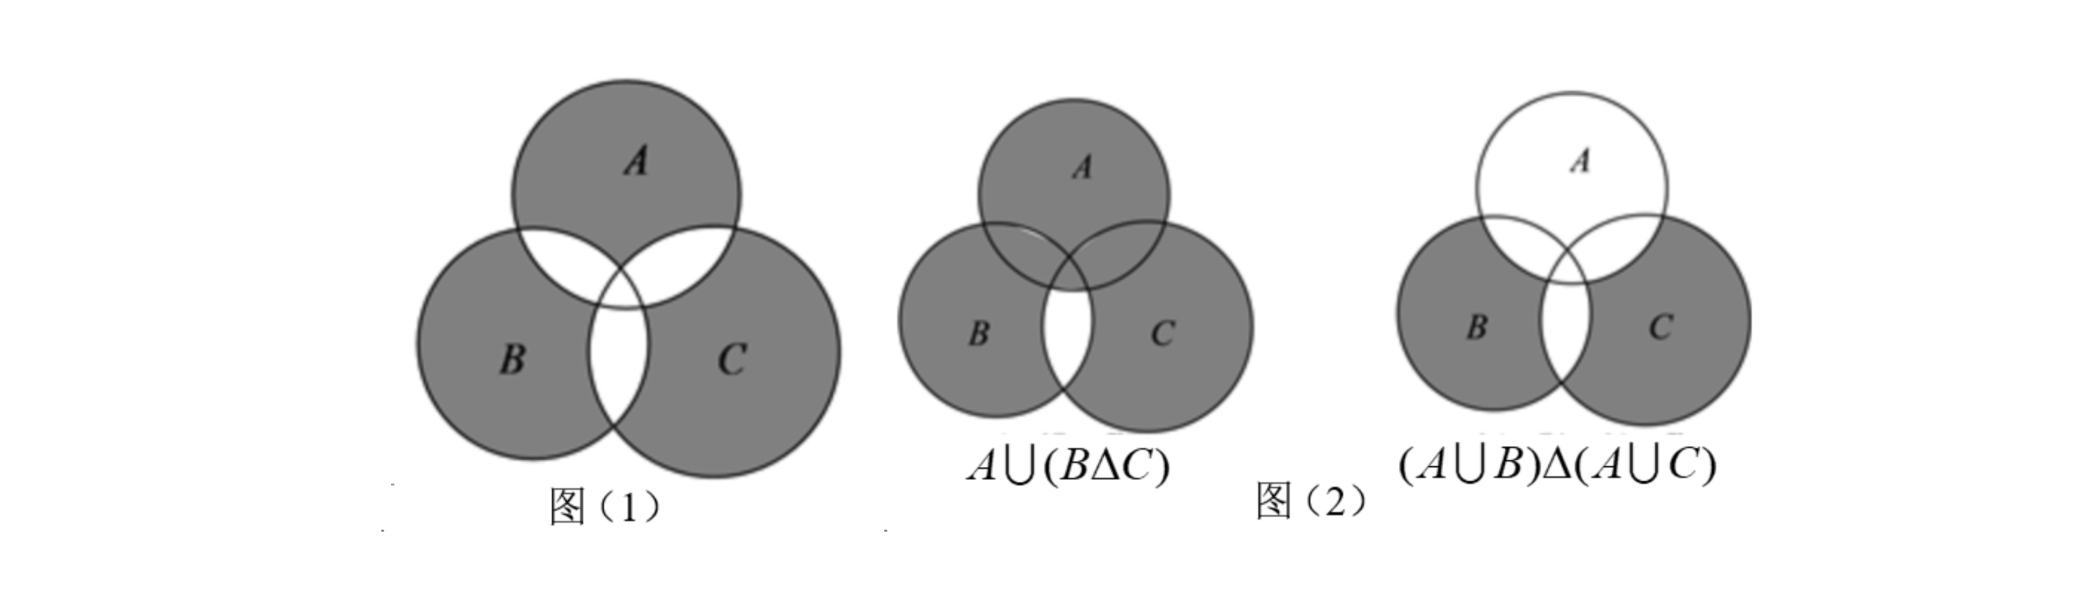
\includegraphics[width=0.92\textwidth]{figures/gao73_q16_symdiff.png}
\end{center}
\step{故选 $B$.}
\solend
\fi

\end{enumerate}

\bigsec{三、解答题}

\begin{enumerate}
\setcounter{enumi}{16}

\item （1）解不等式 $\dfrac{2-x}{x+3}>1$；

（2）已知 $a$ 是实数，试解关于 $x$ 的不等式：$x^2+(a-1)x-a\geqslant0$.

\ifanswer
\solbegin
\stepm{(1)}{$\dfrac{2-x}{x+3}-1=\dfrac{-2x-1}{x+3}>0$，则 $(2x+1)(x+3)<0$，得 $-3<x<-\dfrac12$，}
\step{所以不等式解集为 $\left(-3,-\dfrac12\right)$；}
\stepm{(2)}{$x^2+(a-1)x-a=(x+a)(x-1)\geqslant0$，}
% 原卷 (2) 题干为 ≥0，但解析按 ≤0 给出“两根之间”的解集，照录（见文件头“原卷笔误/存疑”②）
\step{当 $-a<1$，即 $a>-1$ 时，解集为 $(-a,1)$；}
\step{当 $-a=1$，即 $a=-1$ 时，解集为 $\R$；}
\step{当 $-a>1$，即 $a<-1$ 时，解集为 $(1,-a)$；}
\step{综上，当 $a>-1$ 时，解集为 $(-a,1)$；}
\step{当 $a=-1$ 时，解集为 $\R$；}
\step{当 $a<-1$ 时，解集为 $(1,-a)$.}
\solend
\fi

\ansspace[5]

\item （1）设 $a$、$b$ 是两个正数. 已知 $a>b$，比较 $\dfrac{2a+b}{a+2b}$ 与 $\dfrac ab$ 的值的大小；

（2）若实数 $a$ 满足 $\sqrt{(2023-a)^2}+\sqrt{a-2024}=a$，求 $a-2023^2$ 的值.

\ifanswer
\solbegin
\stepm{(1)}{$\dfrac{2a+b}{a+2b}-\dfrac ab=\dfrac{b^2-a^2}{b(a+2b)}<0$，所以 $\dfrac{2a+b}{a+2b}<\dfrac ab$.}
\stepm{(2)}{因为 $a-2024\geqslant0$，所以 $a\geqslant2024$，}
\step{所以 $\sqrt{(2023-a)^2}+\sqrt{a-2024}=a-2023+\sqrt{a-2024}$，}
\step{即 $a-2023+\sqrt{a-2024}=a$，即 $\sqrt{a-2024}=2023$，}
\step{所以 $a-2024=2023^2$，所以 $a-2023^2=2024$.}
\solend
\fi

\ansspace[5]

\item 已知 $m\in\R$，集合 $A=\{x\mid-1\leqslant x\leqslant3\}$，$B=\{x\mid m-3<x\leqslant m+2\}$.

（1）若“$x\in A$”是“$x\in B$”的充分不必要条件，求 $m$ 的取值范围；

（2）若 $A\cap B\neq\varnothing$，求 $m$ 的取值范围.

\ifanswer
\solbegin
\stepm{(1)}{因为“$x\in A$”是“$x\in B$”的充分不必要条件，所以 $A$ 是 $B$ 的真子集，}
\step{需满足 $\begin{cases}m-3<-1\\ m+2\geqslant3\end{cases}$，解得 $\begin{cases}m<2\\ m\geqslant1\end{cases}$，所以 $m$ 的取值范围是 $[1,2)$.}
\stepm{(2)}{因为 $A\cap B\neq\varnothing$，所以 $\begin{cases}m+2\geqslant-1\\ m-3<3\end{cases}$，解得 $\begin{cases}m\geqslant-3\\ m<6\end{cases}$，}
\step{所以 $m$ 的取值范围是 $[-3,6)$.}
\solend
\fi

\ansspace[6]

\item 已知集合 $A=\{x\mid x<-2\text{ 或 }x\geqslant3\}$，$U=\R$.

（1）若 $B=\{x\mid mx-1>0\}$，当 $B\subseteq A$ 时，求实数 $m$ 的取值范围；

（2）若 $B=\{x\mid2m-6\leqslant x\leqslant m+4\}$，当 $B\cap\overline A=\varnothing$ 时，求实数 $m$ 的取值范围.

\ifanswer
\solbegin
\stepm{(1)}{当 $m=0$ 时，$B=\varnothing$，符合题意，}
\step{当 $m>0$ 时，$B=\left\{x\mid x>\dfrac1m\right\}$，则 $\dfrac1m\geqslant3$，解得 $0<m\leqslant\dfrac13$，}
\step{当 $m<0$ 时，$B=\left\{x\mid x<\dfrac1m\right\}$，则 $\dfrac1m\leqslant-2$，解得 $-\dfrac12\leqslant m<0$，}
\step{综上所述，实数 $m$ 的取值范围 $\left[-\dfrac12,\dfrac13\right]$；}
\stepm{(2)}{由题意得 $B=\{x\mid2m-6\leqslant x\leqslant m+4\}$，$\overline A=\{x\mid-2\leqslant x<3\}$，且 $B\cap\overline A=\varnothing$，}
\step{当 $B=\varnothing$ 时，$2m-6>m+4$，解得 $m>10$，}
\step{当 $B\neq\varnothing$ 时，$\begin{cases}2m-6\leqslant m+4\\ m+4<-2\end{cases}$ 或 $\begin{cases}2m-6\leqslant m+4\\ 2m-6\geqslant3\end{cases}$，解得 $m<-6$ 或 $\dfrac92\leqslant m\leqslant10$，}
\step{综上所述，实数 $m$ 的取值范围为 $(-\infty,-6)\cup\left[\dfrac92,+\infty\right)$.}
\solend
\fi

\ansspace[7]

\item 关于实数大小关系的基本事实是解决等式或不等式问题的逻辑基础. 两个正数的大小关系是完全确定的，但通过运算就会产生非常奇妙的变化，基本不等式就是其中之一. 通过运算（代数变形）可以解决很多关于基本不等式的问题.

例如此题：正实数 $x$、$y$，满足 $x+y=1$，求 $\dfrac1x+\dfrac4y$ 的最小值. 求解本问题的方法很多，其中一种求解方法是：$\dfrac1x+\dfrac4y=(x+y)\left(\dfrac1x+\dfrac4y\right)=5+\dfrac yx+\dfrac{4x}{y}\geqslant5+2\sqrt{\dfrac yx\cdot\dfrac{4x}{y}}=9$，当且仅当 $\dfrac yx=\dfrac{4x}{y}$ 即 $y=2x$ 且 $x+y=1$ 时，即 $x=\dfrac13$，$y=\dfrac23$ 时等号成立.

这种解题方法叫作“$1$”的代换，利用上述求解方法解决下列问题：

（1）正数 $a$、$b$ 满足 $a+b=1$，求 $\dfrac1a+\dfrac2b$ 的最小值；

（2）已知 $a$、$b$、$c$ 均为正实数，且 $\dfrac1a+\dfrac1b+\dfrac1c=1$，求证：$a+b+c\geqslant9$；

（3）已知 $a$、$b$、$x$、$y$ 均为正实数，且 $\dfrac{x^2}{a^2}-\dfrac{y^2}{b^2}=1$，求证：$a^2-b^2\leqslant(x-y)^2$.

\ifanswer
\solbegin
\stepm{(1)}{正数 $a$、$b$ 满足 $a+b=1$，}
\step{$\dfrac1a+\dfrac2b=(a+b)\left(\dfrac1a+\dfrac2b\right)=1+2+\dfrac ba+\dfrac{2a}{b}\geqslant3+2\sqrt{\dfrac ba\cdot\dfrac{2a}{b}}=3+2\sqrt2$，}
\step{当且仅当 $\dfrac ba=\dfrac{2a}{b}$ 即 $b=\sqrt2\,a$ 且 $a+b=1$ 时，}
\step{即 $a=\sqrt2-1$，$b=2-\sqrt2$ 时取等号.}
\stepm{(2)}{$a+b+c=\left(\dfrac1a+\dfrac1b+\dfrac1c\right)(a+b+c)=3+\dfrac ba+\dfrac ab+\dfrac ca+\dfrac ac+\dfrac cb+\dfrac bc$}
\step{$\geqslant3+2\sqrt{\dfrac ba\cdot\dfrac ab}+2\sqrt{\dfrac ca\cdot\dfrac ac}+2\sqrt{\dfrac cb\cdot\dfrac bc}=9$，当且仅当 $a=b=c=3$ 时取等号，}
\step{故 $a+b+c\geqslant9$.}
\stepm{(3)}{$a^2-b^2=(a^2-b^2)\left(\dfrac{x^2}{a^2}-\dfrac{y^2}{b^2}\right)=x^2+y^2-\dfrac{b^2x^2}{a^2}-\dfrac{a^2y^2}{b^2}$}
\step{$=x^2+y^2-\left(\dfrac{b^2x^2}{a^2}+\dfrac{a^2y^2}{b^2}\right)\leqslant x^2+y^2-2\cdot\dfrac{bx}{a}\cdot\dfrac{ay}{b}=x^2+y^2-2xy$}
\step{$=(x-y)^2$，当且仅当 $\dfrac{bx}{a}=\dfrac{ay}{b}$ 且 $\dfrac{x^2}{a^2}-\dfrac{y^2}{b^2}=1$ 时，}
\step{即 $x=\dfrac{a^2}{\sqrt{a^2-b^2}}$，$y=\dfrac{b^2}{\sqrt{a^2-b^2}}$，$a>b$ 时取等号，故 $a^2-b^2\leqslant(x-y)^2$.}
\solend
\fi

\ansspace*[7]

\end{enumerate}

\end{document}
"
% 紧凑版：xelatex "\def\iscompact{1}% 高一73_徐汇中学_10月月考.tex
%   —— 高一上数学“2026-2027 年徐汇中学高一上 10 月月考”（讲评版）
% 试卷版：xelatex 高一73_徐汇中学_10月月考.tex
% 答案版：xelatex "\def\isanswer{1}% 高一73_徐汇中学_10月月考.tex
%   —— 高一上数学“2026-2027 年徐汇中学高一上 10 月月考”（讲评版）
% 试卷版：xelatex 高一73_徐汇中学_10月月考.tex
% 答案版：xelatex "\def\isanswer{1}% 高一73_徐汇中学_10月月考.tex
%   —— 高一上数学“2026-2027 年徐汇中学高一上 10 月月考”（讲评版）
% 试卷版：xelatex 高一73_徐汇中学_10月月考.tex
% 答案版：xelatex "\def\isanswer{1}\input{高一73_徐汇中学_10月月考.tex}"
% 紧凑版：xelatex "\def\iscompact{1}\input{高一73_徐汇中学_10月月考.tex}"
%
% 原始材料：微信公众号“魔都数学加油站”文章，连载“27学年高一73”；
% 原文标题“27学年高一73——2026-2027年上海市徐汇中学高一上10月月考”；
% 原文链接：https://mp.weixin.qq.com/s/Pkk9tFr4qHS9BR_BPxvk6A。
% 页面标注发布时间 2026-10-21 20:41（上海）。
% 正文为 10 张 PNG 页（`原图/高一73_徐汇中学_10月月考/01..10.png`）：
% 第 1、4、6、9、10 页为 2560×3620，其余 5 页为 4762×6735，均按页序读取。
% 10 页全为试卷正文页（卷首标题在第 1 页页顶，卷末第 21 题 (3) 解析止于第 10 页），
% 无封面页、目录页、二维码或宣传页。粉色斜排“魔都数学加油站”为卷面水印，未录入。
%
% 卷首标题：照卷面印作“2026-2027 年徐汇中学高一上 10 月月考”（黑体加粗一行）。
% 原卷年份区间用半角连字符，本稿按全稿惯例排 en dash；原卷无副标题。
%
% 篇幅与题号：原卷自第 3 题起编号（第 1、2 题不在本卷内）。填空题 3—12（10 题）、
% 选择题 13—16（4 题）、解答题 17—21（5 题），共 19 题。本稿沿用原节与原题号，
% 只改排为全稿统一的大节样式。
%
% 讲评版：原卷第 3、4 题只印【答案】（“没有实数根”“真”），本稿只给 \ans{}；
% 其余 17 题均印【解析】，用 \solbegin…\solend。四道选择题的作答括号原卷即留空，
% 答案写在解析末句“故选 A／D／A／B”，照录在解析内，不另提 \ans{}。
%
% 副标题：原卷未印副标题。本稿按“知识模块”口径标作“集合与常用逻辑用语、不等式”：
% 19 题中集合与常用逻辑用语 9 题（第 3、4、7、11、12、13、16、19、20 题），
% 不等式 10 题（第 5、6、8、9、10、14、15、17、18、21 题），两类均确有分量，故并标。
% 口径同 高一63、高一68—72。
%
% 与原卷的排版差异：
%   ① 原卷每题下直接印【答案】/【解析】，本稿按全稿惯例将答案与解析置于答案版；
%   ② 原卷未印副标题，本稿按“知识模块”口径补出；
%   ③ 原卷填空横线约四个字宽，本稿按全稿惯例统一排 \blankline[4.4em]；
%   ④ 原卷数集记号排斜体 $R$（第 3、8、9、10、12、17、19、20 题等），本稿按全稿惯例
%      改用 $\R$（同 高一68—72）；空集记号原卷作 $\varnothing$，照录；
%   ⑤ 原卷句末标点多为西文句点，第 15 题题干“整数解只有 $-2$”后为全角逗号，
%      均逐处照录；第 16 题解析的集合运算用 $\Delta$ 表示对称差，照原卷符号排；
%   ⑥ 第 17—21 题的子问原卷印作“（1）…（2）…”，本稿按 高一69—72 成例用行内
%      “（1）（2）（3）”段，解析中的子问标号用 \stepm{(1)}{…}；
%   ⑦ 每道解答题原卷未留作答空白，本稿按全稿惯例加 \ansspace（末题用 \ansspace*）；
%   ⑧ 选择题的作答括号原卷排半角“(    )”，本稿按全稿惯例排 \mbox{（\quad）}；
%      选项行排照原卷——第 13 题一行四条、第 14—16 题一行四条；
%   ⑨ 第 15 题题干的不等式组、第 14、19、20 题解析中的不等式组，原卷均排作“{”
%      连接的多行式，本稿按全稿惯例排 cases；
%   ⑩ 第 16 题解析末尾有三幅韦恩图（图（1）与图（2）的两幅）：原卷印在【解析】中，
%      题干无“如图”二字。本稿按原卷截图裁取（`figures/gao73_q16_symdiff.png`，
%      由第 6 页原图裁出、去除粉色水印后转灰度，未放大），放在答案版解析④之后。
%
% 原卷笔误/存疑（均照录未改，正文对应处另有 % 注）：
%   ① 第 3 题题干“设 $a$、$b\in\R$，则方程 $x^2+ax+a-1=0$ 至少有一个实根”中
%      $b$ 未在方程或后文出现，疑为衍字；原卷如此，照录未改。
%   ② 第 17 题 (2) 题干为 $x^2+(a-1)x-a\geqslant0$，但解析按 $\leqslant0$ 给出解集：
%      $a>-1$ 时写 $(-a,1)$、$a<-1$ 时写 $(1,-a)$，恰是“两根之间”的区间。
%      按题干 $\geqslant0$ 应为 $(-\infty,-a]\cup[1,+\infty)$ 与 $(-\infty,1]\cup[-a,+\infty)$；
%      原卷如此，照录未改。
%
% 行数核对：逐题数 \step/\stepm 条数与原卷【解析】印刷行数，17 题逐一相符，
% 合计 104 条 / 104 行（Q5：1；Q6：2；Q7：4；Q8：4；Q9：3；Q10：4；Q11：8；
% Q12：7；Q13：7；Q14：5；Q15：7；Q16：15；Q17：9；Q18：5；Q19：4；Q20：8；Q21：11）。
% 另第 3、4 题只印【答案】，各提 \ans{}，不计入 \step 账。
%
% 插图：第 16 题解析末的 3 幅韦恩图，见上⑩；全卷题干无其他配图。
%
\documentclass[a4paper,11pt]{article}
\usepackage{common}

\begin{document}

\examtitlest[3]{2026--2027 年徐汇中学高一上 10 月月考}{集合与常用逻辑用语、不等式}

\bigsec{一、填空题}

\begin{enumerate}
\setcounter{enumi}{2}

% 原卷题干“设 a、b∈R”中的 b 未在方程中出现，照录（见文件头“原卷笔误/存疑”①）
\item 如果用反证法证明命题“设 $a$、$b\in\R$，则方程 $x^2+ax+a-1=0$ 至少有一个实根”，那么首先假设方程 $x^2+ax+a-1=0$\blankline[4.4em].

\ifanswer
\ans{没有实数根}
\fi

\item 命题“若 $\dfrac1x>1$，则 $x<1$”是\blankline[4.4em]命题（填“真”，“假”）.

\ifanswer
\ans{真}
\fi

\item 对数 $\log_a(5-a)$ 中实数 $a$ 的取值范围是\blankline[4.4em].

\ifanswer
\solbegin
\step{由对数定义得 $\begin{cases}a>0\\ a\neq1\\ 5-a>0\end{cases}$，解得 $0<a<1$ 或 $1<a<5$.}
\solend
\fi

\item 关于 $x$ 的不等式 $ax^2-(a+1)x+1\leqslant0\,(a<0)$ 的解集为\blankline[4.4em].

\ifanswer
\solbegin
\step{原不等式即 $(ax-1)(x-1)\leqslant0$，因为 $a<0$，所以 $\left(x-\dfrac1a\right)(x-1)\geqslant0$.}
\step{又 $\dfrac1a<0<1$，所以 $x\leqslant\dfrac1a$ 或 $x\geqslant1$，故解集为 $\left(-\infty,\dfrac1a\right]\cup[1,+\infty)$.}
\solend
\fi

\item 若集合 $A=\{x\mid x^2-2kx+7k=0\}$ 有且仅有三个真子集，则 $k$ 的取值范围是\blankline[4.4em].

\ifanswer
\solbegin
\step{因为集合 $A$ 有且仅有三个真子集，则 $2^n-1=3$，解得 $n=2$，}
\step{所以一元二次方程 $x^2-2kx+7k=0$ 有两个不同的实数解，}
\step{则 $\Delta=4k^2-28k>0$，解得 $k<0$ 或 $k>7$，}
\step{故 $k$ 的取值范围是 $(-\infty,0)\cup(7,+\infty)$.}
\solend
\fi

\item 已知关于 $x$ 的不等式 $kx^2-4kx+k-6<0$ 对任意 $x\in\R$ 恒成立，则 $k$ 的取值范围是\blankline[4.4em].

\ifanswer
\solbegin
\step{关于 $x$ 的不等式 $kx^2-4kx+k-6<0$ 对任意 $x\in\R$ 恒成立，}
\step{当 $k=0$ 时，$kx^2-4kx+k-6=-6<0$ 恒成立，}
\step{当 $k\neq0$ 时，则 $\begin{cases}\Delta=16k^2-4k(k-6)<0\\ k<0\end{cases}$，解得 $-2<k<0$，}
\step{综上，$k$ 的取值范围为 $(-2,0]$.}
\solend
\fi

\item 设 $x\in\R$，方程 $|x-1|+|2x-1|=|3x-2|$ 的解集为\blankline[4.4em].

\ifanswer
\solbegin
\step{因为 $|x-1|+|2x-1|\geqslant|(x-1)+(2x-1)|=|3x-2|$，}
\step{当且仅当 $(x-1)(2x-1)\geqslant0$，解得 $x\leqslant\dfrac12$ 或 $x\geqslant1$，}
\step{故方程 $|x-1|+|2x-1|=|3x-2|$ 的解集为 $\left(-\infty,\dfrac12\right]\cup[1,+\infty)$.}
\solend
\fi

\item 已知 $a\in\R$，若关于 $x$ 的方程 $x^2+ax+a^2-8=0$ 有两个实根 $x_1$、$x_2$，且 $\dfrac1{x_1}+\dfrac1{x_2}=-\dfrac12$，则 $a$ 的值为\blankline[4.4em].

\ifanswer
\solbegin
\step{由题意得 $\Delta=a^2-4(a^2-8)=32-3a^2\geqslant0$，解得 $a^2\leqslant\dfrac{32}3$，}
\step{由韦达定理得 $x_1+x_2=-a$，$x_1x_2=a^2-8$，}
\step{则 $\dfrac1{x_1}+\dfrac1{x_2}=\dfrac{x_1+x_2}{x_1x_2}=\dfrac{-a}{a^2-8}=-\dfrac12$，即 $a^2-2a-8=(a-4)(a+2)=0$，}
\step{解得 $a=4$ 或 $a=-2$. 又 $a^2\leqslant\dfrac{32}3$，则 $a=-2$.}
\solend
\fi

\item 甲、乙两人解关于 $x$ 的不等式 $x^2+bx+c<0$，甲写错了 $b$，正确计算后得到的解为 $\{x\mid1<x<2\}$；乙写错了 $c$，正确计算后得到的解为 $\{x\mid-4<x<1\}$. 那么不等式 $\dfrac{bx+c}{x-2}<0$ 的解为\blankline[4.4em].

\ifanswer
\solbegin
\step{由 $x^2+bx+c<0$ 的解为 $\{x\mid1<x<2\}$，}
\step{则 $1$ 和 $2$ 是方程 $x^2+bx+c=0$ 的两个根，}
\step{甲写错了 $b$，但 $c$ 是正确的，所以 $c=1\times2=2$；}
\step{由 $x^2+bx+c<0$ 的解为 $\{x\mid-4<x<1\}$，}
\step{则 $-4$ 和 $1$ 是方程 $x^2+bx+c=0$ 的两个根，}
\step{乙写错了 $c$，但 $b$ 是正确的，所以 $-b=-4+1=-3$，即 $b=3$.}
\step{由 $\dfrac{bx+c}{x-2}<0$，得 $\dfrac{3x+2}{x-2}<0$，即 $(3x+2)(x-2)<0$，解得 $-\dfrac23<x<2$，}
\step{所以不等式 $\dfrac{bx+c}{x-2}<0$ 的解为 $\left\{x\mid-\dfrac23<x<2\right\}$.}
\solend
\fi

\item 设 $a,b,c\in\R$，$S=\{x\mid(x+a)(x^2+bx+c)=0,x\in\R\}$，$T=\{x\mid(ax+1)(cx^2+bx+1)=0,x\in\R\}$. 若 $|S|$、$|T|$ 分别为集合 $S$、$T$ 的元素个数，则 $|S|+|T|$ 的所有可能取值组成的集合为\blankline[4.4em].

\ifanswer
\solbegin
\step{$x\neq0$ 时，$(ax+1)(cx^2+bx+1)=x^3\left(\dfrac1x+a\right)\left(\dfrac1{x^2}+\dfrac bx+c\right)$，}
\step{故 $S$、$T$ 的非零元按倒数一一对应，设其个数均为 $k$；}
\step{$0\notin T$，且 $0\in S\Leftrightarrow ac=0$. 当 $ac=0$ 时 $k\in\{0,1,2\}$，}
\step{当 $ac\neq0$ 时 $x=-a\neq0$ 是 $S$ 的非零元，$k\in\{1,2,3\}$.}
\step{因此 $|S|+|T|$ 分别可取 $2k+1\in\{1,3,5\}$ 与 $2k\in\{2,4,6\}$.}
\step{依次取 $(a,b,c)=(0,0,0),(1,0,1),(0,-2,1),(1,-2,1),(0,0,-1),(1,-5,6)$，可分别实现 $1,2,3,4,5,6$，}
\step{则 $|S|+|T|$ 的所有可能取值组成的集合为 $\{1,2,3,4,5,6\}$.}
\solend
\fi

\end{enumerate}

\bigsec{二、选择题}

\begin{enumerate}
\setcounter{enumi}{12}

\item 如果 $a>b$，$c\neq0$，那么下列不等式成立的是\mbox{（\quad）}

\keepwithprev
A. $a-c>b-c$\qquad B. $c-a>c-b$\qquad C. $ac>bc$\qquad D. $\dfrac ac>\dfrac bc$

\ifanswer
\solbegin
\step{对于 $A$：$a-c-(b-c)=a-b>0$，即 $a-c>b-c$，故 $A$ 正确；}
\step{对于 $B$：$c-a-(c-b)=b-a<0$，即 $c-a<c-b$，故 $B$ 错误；}
\step{对于 $C$：$ac-bc=c(a-b)$，已知 $a-b>0$，}
\step{当 $c<0$ 时，$c(a-b)<0$，此时 $ac<bc$，故 $C$ 错误；}
\step{对于 $D$：$\dfrac ac-\dfrac bc=\dfrac1c(a-b)$，已知 $a-b>0$，}
\step{当 $c<0$ 时，$\dfrac1c(a-b)<0$，此时 $\dfrac ac<\dfrac bc$，故 $D$ 错误.}
\step{故选 $A$.}
\solend
\fi

\item 若不等式 $|x+1|\leqslant a$ 成立的一个充分不必要条件是 $-3\leqslant x\leqslant4$，则整数 $a$ 的最小值为\mbox{（\quad）}

\keepwithprev
A. $2$\qquad B. $3$\qquad C. $4$\qquad D. $5$

\ifanswer
\solbegin
\step{若 $a<0$，则 $|x+1|\leqslant a$ 无解；}
\step{若 $a\geqslant0$，由 $|x+1|\leqslant a$，得 $-1-a\leqslant x\leqslant-1+a$，}
\step{因为 $|x+1|\leqslant a$ 成立的一个充分不必要条件是 $-3\leqslant x\leqslant4$，}
\step{所以 $\begin{cases}-1-a\leqslant-3\\ -1+a\geqslant4\end{cases}$，等号不同时成立，解得 $a\geqslant5$，}
\step{故整数 $a$ 的最小值为 $5$. 故选 $D$.}
\solend
\fi

\item 若关于 $x$ 的不等式组 $\begin{cases}x^2-x-2>0\\ 2x^2+(5+2k)x+5k<0\end{cases}$ 的整数解只有 $-2$，则实数 $k$ 的取值范围为\mbox{（\quad）}

\keepwithprev
A. $[-3,2)$\qquad B. $[1,2]$\qquad C. $(1,2]$\qquad D. $(1,2)$

\ifanswer
\solbegin
\step{由 $x^2-x-2>0$，得 $x>2$ 或 $x<-1$，}
\step{由 $2x^2+(2k+5)x+5k<0$，得 $(2x+5)(x+k)<0$.}
\step{①若 $-k<-\dfrac52$，即 $k>\dfrac52$ 时，解得 $-k<x<-\dfrac52$，}
\step{此时原不等式的解集为 $\left(-k,-\dfrac52\right)$，不符合题意；}
\step{②若 $k=\dfrac52$ 时，解得 $x\in\varnothing$，显然不符合题意；}
\step{③若 $k<\dfrac52$ 时，解得 $-\dfrac52<x<-k$，则 $-2<-k\leqslant3$，即 $-3\leqslant k<2$.}
\step{综上，实数 $k$ 的取值范围 $[-3,2)$. 故选 $A$.}
\solend
\fi

\item 定义集合运算 $A-B=\{x\mid x\in A\text{ 且 }x\notin B\}$ 称为集合 $A$ 与集合 $B$ 的差集；定义集合运算 $A\Delta B=(A-B)\cup(B-A)$ 称为集合 $A$ 与集合 $B$ 的对称差，有以下 $4$ 个等式：

① $A\Delta B=B\Delta A$；

② $(A\Delta B)\Delta C=A\Delta(B\Delta C)$；

③ $A\cap(B\Delta C)=(A\cap B)\Delta(A\cap C)$；

④ $A\cup(B\Delta C)=(A\cup B)\Delta(A\cup C)$.

则 $4$ 个等式中恒成立的是\mbox{（\quad）}

\keepwithprev
A. ①②\qquad B. ①②③\qquad C. ①②④\qquad D. ①②③④

\ifanswer
\solbegin
\step{对于①，由 $B\Delta A=(B-A)\cup(A-B)=(A-B)\cup(B-A)=A\Delta B$，}
\step{所以①正确；}
\step{对于②，}
\step{由 $A-B=\{x\mid x\in A\text{ 且 }x\notin B\}=\{x\mid x\in A,x\notin(A\cap B)\}=A-(A\cap B)$，}
\step{同理可得 $B-A=B-(A\cap B)$，}
\step{则 $A\Delta B=(A-B)\cup(B-A)=(A\cup B)-(A\cap B)$，}
\step{所以 $(A\Delta B)\Delta C=(A\Delta B)\cup C-(A\Delta B)\cap C$，}
\step{所以表示的集合为图（1）中阴影部分所表示的集合，如图所示，}
\step{同理 $A\Delta(B\Delta C)=A\cup(B\Delta C)-A\cap(B\Delta C)$，}
\step{也表示图（1）中阴影部分所表示的集合，}
\step{所以 $(A\Delta B)\Delta C=A\Delta(B\Delta C)$，所以②正确；}
\step{对于③，由 $A\cap(B\Delta C)=A\cap(B\cup C-B\cap C)=A\cap(B\cup C)-A\cap(B\cap C)$}
\step{$=(A\cap B)\cup(A\cap C)-(A\cap B)\cap(A\cap C)=(A\cap B)\Delta(A\cap C)$，所以③正确；}
\step{对于④，如图（2）所示，$A\cup(B\Delta C)\neq(A\cup B)\Delta(A\cup C)$，所以④错误.}
\begin{center}
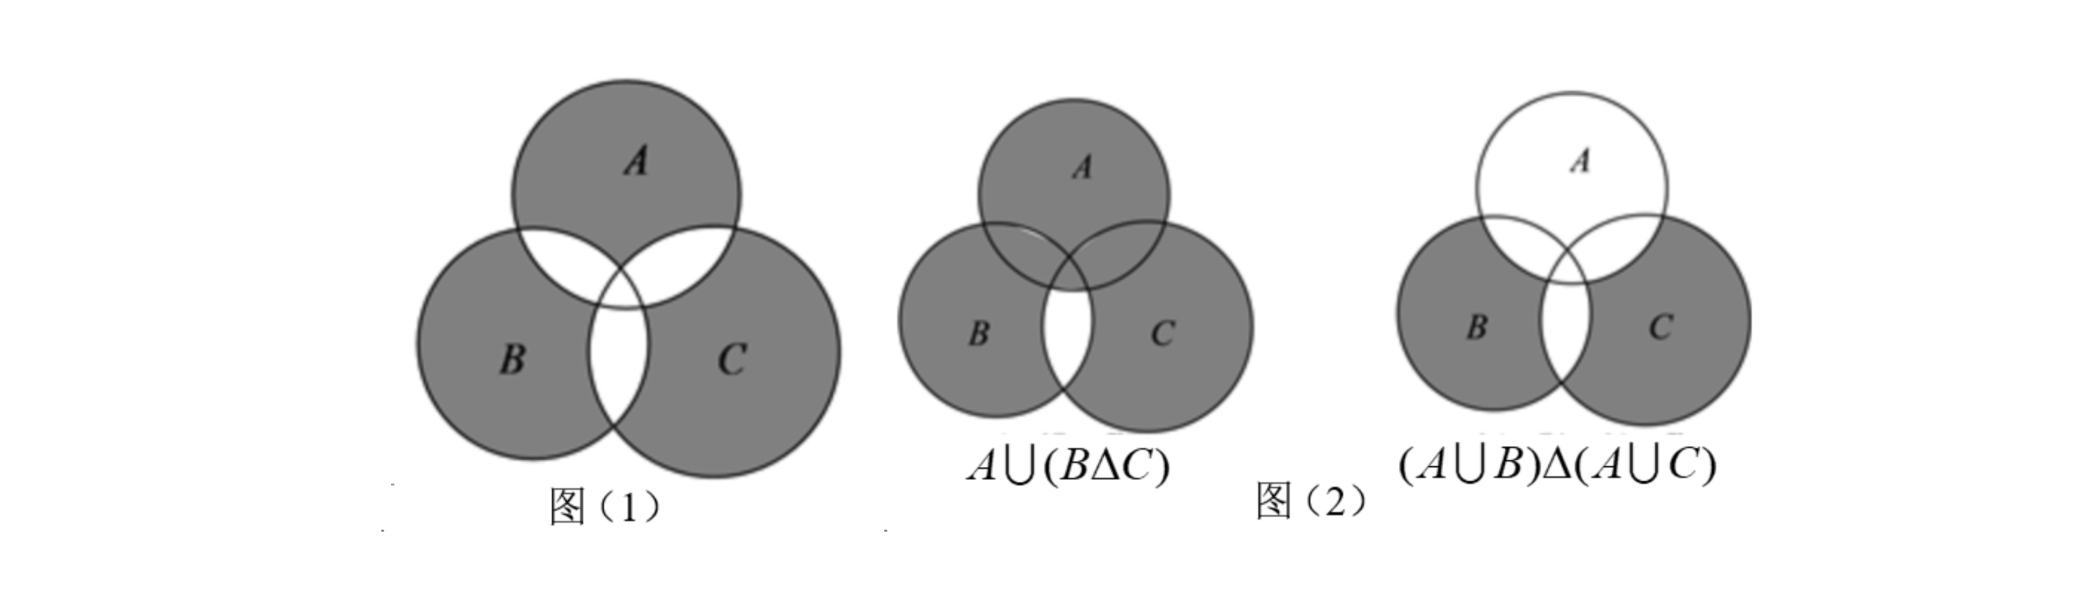
\includegraphics[width=0.92\textwidth]{figures/gao73_q16_symdiff.png}
\end{center}
\step{故选 $B$.}
\solend
\fi

\end{enumerate}

\bigsec{三、解答题}

\begin{enumerate}
\setcounter{enumi}{16}

\item （1）解不等式 $\dfrac{2-x}{x+3}>1$；

（2）已知 $a$ 是实数，试解关于 $x$ 的不等式：$x^2+(a-1)x-a\geqslant0$.

\ifanswer
\solbegin
\stepm{(1)}{$\dfrac{2-x}{x+3}-1=\dfrac{-2x-1}{x+3}>0$，则 $(2x+1)(x+3)<0$，得 $-3<x<-\dfrac12$，}
\step{所以不等式解集为 $\left(-3,-\dfrac12\right)$；}
\stepm{(2)}{$x^2+(a-1)x-a=(x+a)(x-1)\geqslant0$，}
% 原卷 (2) 题干为 ≥0，但解析按 ≤0 给出“两根之间”的解集，照录（见文件头“原卷笔误/存疑”②）
\step{当 $-a<1$，即 $a>-1$ 时，解集为 $(-a,1)$；}
\step{当 $-a=1$，即 $a=-1$ 时，解集为 $\R$；}
\step{当 $-a>1$，即 $a<-1$ 时，解集为 $(1,-a)$；}
\step{综上，当 $a>-1$ 时，解集为 $(-a,1)$；}
\step{当 $a=-1$ 时，解集为 $\R$；}
\step{当 $a<-1$ 时，解集为 $(1,-a)$.}
\solend
\fi

\ansspace[5]

\item （1）设 $a$、$b$ 是两个正数. 已知 $a>b$，比较 $\dfrac{2a+b}{a+2b}$ 与 $\dfrac ab$ 的值的大小；

（2）若实数 $a$ 满足 $\sqrt{(2023-a)^2}+\sqrt{a-2024}=a$，求 $a-2023^2$ 的值.

\ifanswer
\solbegin
\stepm{(1)}{$\dfrac{2a+b}{a+2b}-\dfrac ab=\dfrac{b^2-a^2}{b(a+2b)}<0$，所以 $\dfrac{2a+b}{a+2b}<\dfrac ab$.}
\stepm{(2)}{因为 $a-2024\geqslant0$，所以 $a\geqslant2024$，}
\step{所以 $\sqrt{(2023-a)^2}+\sqrt{a-2024}=a-2023+\sqrt{a-2024}$，}
\step{即 $a-2023+\sqrt{a-2024}=a$，即 $\sqrt{a-2024}=2023$，}
\step{所以 $a-2024=2023^2$，所以 $a-2023^2=2024$.}
\solend
\fi

\ansspace[5]

\item 已知 $m\in\R$，集合 $A=\{x\mid-1\leqslant x\leqslant3\}$，$B=\{x\mid m-3<x\leqslant m+2\}$.

（1）若“$x\in A$”是“$x\in B$”的充分不必要条件，求 $m$ 的取值范围；

（2）若 $A\cap B\neq\varnothing$，求 $m$ 的取值范围.

\ifanswer
\solbegin
\stepm{(1)}{因为“$x\in A$”是“$x\in B$”的充分不必要条件，所以 $A$ 是 $B$ 的真子集，}
\step{需满足 $\begin{cases}m-3<-1\\ m+2\geqslant3\end{cases}$，解得 $\begin{cases}m<2\\ m\geqslant1\end{cases}$，所以 $m$ 的取值范围是 $[1,2)$.}
\stepm{(2)}{因为 $A\cap B\neq\varnothing$，所以 $\begin{cases}m+2\geqslant-1\\ m-3<3\end{cases}$，解得 $\begin{cases}m\geqslant-3\\ m<6\end{cases}$，}
\step{所以 $m$ 的取值范围是 $[-3,6)$.}
\solend
\fi

\ansspace[6]

\item 已知集合 $A=\{x\mid x<-2\text{ 或 }x\geqslant3\}$，$U=\R$.

（1）若 $B=\{x\mid mx-1>0\}$，当 $B\subseteq A$ 时，求实数 $m$ 的取值范围；

（2）若 $B=\{x\mid2m-6\leqslant x\leqslant m+4\}$，当 $B\cap\overline A=\varnothing$ 时，求实数 $m$ 的取值范围.

\ifanswer
\solbegin
\stepm{(1)}{当 $m=0$ 时，$B=\varnothing$，符合题意，}
\step{当 $m>0$ 时，$B=\left\{x\mid x>\dfrac1m\right\}$，则 $\dfrac1m\geqslant3$，解得 $0<m\leqslant\dfrac13$，}
\step{当 $m<0$ 时，$B=\left\{x\mid x<\dfrac1m\right\}$，则 $\dfrac1m\leqslant-2$，解得 $-\dfrac12\leqslant m<0$，}
\step{综上所述，实数 $m$ 的取值范围 $\left[-\dfrac12,\dfrac13\right]$；}
\stepm{(2)}{由题意得 $B=\{x\mid2m-6\leqslant x\leqslant m+4\}$，$\overline A=\{x\mid-2\leqslant x<3\}$，且 $B\cap\overline A=\varnothing$，}
\step{当 $B=\varnothing$ 时，$2m-6>m+4$，解得 $m>10$，}
\step{当 $B\neq\varnothing$ 时，$\begin{cases}2m-6\leqslant m+4\\ m+4<-2\end{cases}$ 或 $\begin{cases}2m-6\leqslant m+4\\ 2m-6\geqslant3\end{cases}$，解得 $m<-6$ 或 $\dfrac92\leqslant m\leqslant10$，}
\step{综上所述，实数 $m$ 的取值范围为 $(-\infty,-6)\cup\left[\dfrac92,+\infty\right)$.}
\solend
\fi

\ansspace[7]

\item 关于实数大小关系的基本事实是解决等式或不等式问题的逻辑基础. 两个正数的大小关系是完全确定的，但通过运算就会产生非常奇妙的变化，基本不等式就是其中之一. 通过运算（代数变形）可以解决很多关于基本不等式的问题.

例如此题：正实数 $x$、$y$，满足 $x+y=1$，求 $\dfrac1x+\dfrac4y$ 的最小值. 求解本问题的方法很多，其中一种求解方法是：$\dfrac1x+\dfrac4y=(x+y)\left(\dfrac1x+\dfrac4y\right)=5+\dfrac yx+\dfrac{4x}{y}\geqslant5+2\sqrt{\dfrac yx\cdot\dfrac{4x}{y}}=9$，当且仅当 $\dfrac yx=\dfrac{4x}{y}$ 即 $y=2x$ 且 $x+y=1$ 时，即 $x=\dfrac13$，$y=\dfrac23$ 时等号成立.

这种解题方法叫作“$1$”的代换，利用上述求解方法解决下列问题：

（1）正数 $a$、$b$ 满足 $a+b=1$，求 $\dfrac1a+\dfrac2b$ 的最小值；

（2）已知 $a$、$b$、$c$ 均为正实数，且 $\dfrac1a+\dfrac1b+\dfrac1c=1$，求证：$a+b+c\geqslant9$；

（3）已知 $a$、$b$、$x$、$y$ 均为正实数，且 $\dfrac{x^2}{a^2}-\dfrac{y^2}{b^2}=1$，求证：$a^2-b^2\leqslant(x-y)^2$.

\ifanswer
\solbegin
\stepm{(1)}{正数 $a$、$b$ 满足 $a+b=1$，}
\step{$\dfrac1a+\dfrac2b=(a+b)\left(\dfrac1a+\dfrac2b\right)=1+2+\dfrac ba+\dfrac{2a}{b}\geqslant3+2\sqrt{\dfrac ba\cdot\dfrac{2a}{b}}=3+2\sqrt2$，}
\step{当且仅当 $\dfrac ba=\dfrac{2a}{b}$ 即 $b=\sqrt2\,a$ 且 $a+b=1$ 时，}
\step{即 $a=\sqrt2-1$，$b=2-\sqrt2$ 时取等号.}
\stepm{(2)}{$a+b+c=\left(\dfrac1a+\dfrac1b+\dfrac1c\right)(a+b+c)=3+\dfrac ba+\dfrac ab+\dfrac ca+\dfrac ac+\dfrac cb+\dfrac bc$}
\step{$\geqslant3+2\sqrt{\dfrac ba\cdot\dfrac ab}+2\sqrt{\dfrac ca\cdot\dfrac ac}+2\sqrt{\dfrac cb\cdot\dfrac bc}=9$，当且仅当 $a=b=c=3$ 时取等号，}
\step{故 $a+b+c\geqslant9$.}
\stepm{(3)}{$a^2-b^2=(a^2-b^2)\left(\dfrac{x^2}{a^2}-\dfrac{y^2}{b^2}\right)=x^2+y^2-\dfrac{b^2x^2}{a^2}-\dfrac{a^2y^2}{b^2}$}
\step{$=x^2+y^2-\left(\dfrac{b^2x^2}{a^2}+\dfrac{a^2y^2}{b^2}\right)\leqslant x^2+y^2-2\cdot\dfrac{bx}{a}\cdot\dfrac{ay}{b}=x^2+y^2-2xy$}
\step{$=(x-y)^2$，当且仅当 $\dfrac{bx}{a}=\dfrac{ay}{b}$ 且 $\dfrac{x^2}{a^2}-\dfrac{y^2}{b^2}=1$ 时，}
\step{即 $x=\dfrac{a^2}{\sqrt{a^2-b^2}}$，$y=\dfrac{b^2}{\sqrt{a^2-b^2}}$，$a>b$ 时取等号，故 $a^2-b^2\leqslant(x-y)^2$.}
\solend
\fi

\ansspace*[7]

\end{enumerate}

\end{document}
"
% 紧凑版：xelatex "\def\iscompact{1}% 高一73_徐汇中学_10月月考.tex
%   —— 高一上数学“2026-2027 年徐汇中学高一上 10 月月考”（讲评版）
% 试卷版：xelatex 高一73_徐汇中学_10月月考.tex
% 答案版：xelatex "\def\isanswer{1}\input{高一73_徐汇中学_10月月考.tex}"
% 紧凑版：xelatex "\def\iscompact{1}\input{高一73_徐汇中学_10月月考.tex}"
%
% 原始材料：微信公众号“魔都数学加油站”文章，连载“27学年高一73”；
% 原文标题“27学年高一73——2026-2027年上海市徐汇中学高一上10月月考”；
% 原文链接：https://mp.weixin.qq.com/s/Pkk9tFr4qHS9BR_BPxvk6A。
% 页面标注发布时间 2026-10-21 20:41（上海）。
% 正文为 10 张 PNG 页（`原图/高一73_徐汇中学_10月月考/01..10.png`）：
% 第 1、4、6、9、10 页为 2560×3620，其余 5 页为 4762×6735，均按页序读取。
% 10 页全为试卷正文页（卷首标题在第 1 页页顶，卷末第 21 题 (3) 解析止于第 10 页），
% 无封面页、目录页、二维码或宣传页。粉色斜排“魔都数学加油站”为卷面水印，未录入。
%
% 卷首标题：照卷面印作“2026-2027 年徐汇中学高一上 10 月月考”（黑体加粗一行）。
% 原卷年份区间用半角连字符，本稿按全稿惯例排 en dash；原卷无副标题。
%
% 篇幅与题号：原卷自第 3 题起编号（第 1、2 题不在本卷内）。填空题 3—12（10 题）、
% 选择题 13—16（4 题）、解答题 17—21（5 题），共 19 题。本稿沿用原节与原题号，
% 只改排为全稿统一的大节样式。
%
% 讲评版：原卷第 3、4 题只印【答案】（“没有实数根”“真”），本稿只给 \ans{}；
% 其余 17 题均印【解析】，用 \solbegin…\solend。四道选择题的作答括号原卷即留空，
% 答案写在解析末句“故选 A／D／A／B”，照录在解析内，不另提 \ans{}。
%
% 副标题：原卷未印副标题。本稿按“知识模块”口径标作“集合与常用逻辑用语、不等式”：
% 19 题中集合与常用逻辑用语 9 题（第 3、4、7、11、12、13、16、19、20 题），
% 不等式 10 题（第 5、6、8、9、10、14、15、17、18、21 题），两类均确有分量，故并标。
% 口径同 高一63、高一68—72。
%
% 与原卷的排版差异：
%   ① 原卷每题下直接印【答案】/【解析】，本稿按全稿惯例将答案与解析置于答案版；
%   ② 原卷未印副标题，本稿按“知识模块”口径补出；
%   ③ 原卷填空横线约四个字宽，本稿按全稿惯例统一排 \blankline[4.4em]；
%   ④ 原卷数集记号排斜体 $R$（第 3、8、9、10、12、17、19、20 题等），本稿按全稿惯例
%      改用 $\R$（同 高一68—72）；空集记号原卷作 $\varnothing$，照录；
%   ⑤ 原卷句末标点多为西文句点，第 15 题题干“整数解只有 $-2$”后为全角逗号，
%      均逐处照录；第 16 题解析的集合运算用 $\Delta$ 表示对称差，照原卷符号排；
%   ⑥ 第 17—21 题的子问原卷印作“（1）…（2）…”，本稿按 高一69—72 成例用行内
%      “（1）（2）（3）”段，解析中的子问标号用 \stepm{(1)}{…}；
%   ⑦ 每道解答题原卷未留作答空白，本稿按全稿惯例加 \ansspace（末题用 \ansspace*）；
%   ⑧ 选择题的作答括号原卷排半角“(    )”，本稿按全稿惯例排 \mbox{（\quad）}；
%      选项行排照原卷——第 13 题一行四条、第 14—16 题一行四条；
%   ⑨ 第 15 题题干的不等式组、第 14、19、20 题解析中的不等式组，原卷均排作“{”
%      连接的多行式，本稿按全稿惯例排 cases；
%   ⑩ 第 16 题解析末尾有三幅韦恩图（图（1）与图（2）的两幅）：原卷印在【解析】中，
%      题干无“如图”二字。本稿按原卷截图裁取（`figures/gao73_q16_symdiff.png`，
%      由第 6 页原图裁出、去除粉色水印后转灰度，未放大），放在答案版解析④之后。
%
% 原卷笔误/存疑（均照录未改，正文对应处另有 % 注）：
%   ① 第 3 题题干“设 $a$、$b\in\R$，则方程 $x^2+ax+a-1=0$ 至少有一个实根”中
%      $b$ 未在方程或后文出现，疑为衍字；原卷如此，照录未改。
%   ② 第 17 题 (2) 题干为 $x^2+(a-1)x-a\geqslant0$，但解析按 $\leqslant0$ 给出解集：
%      $a>-1$ 时写 $(-a,1)$、$a<-1$ 时写 $(1,-a)$，恰是“两根之间”的区间。
%      按题干 $\geqslant0$ 应为 $(-\infty,-a]\cup[1,+\infty)$ 与 $(-\infty,1]\cup[-a,+\infty)$；
%      原卷如此，照录未改。
%
% 行数核对：逐题数 \step/\stepm 条数与原卷【解析】印刷行数，17 题逐一相符，
% 合计 104 条 / 104 行（Q5：1；Q6：2；Q7：4；Q8：4；Q9：3；Q10：4；Q11：8；
% Q12：7；Q13：7；Q14：5；Q15：7；Q16：15；Q17：9；Q18：5；Q19：4；Q20：8；Q21：11）。
% 另第 3、4 题只印【答案】，各提 \ans{}，不计入 \step 账。
%
% 插图：第 16 题解析末的 3 幅韦恩图，见上⑩；全卷题干无其他配图。
%
\documentclass[a4paper,11pt]{article}
\usepackage{common}

\begin{document}

\examtitlest[3]{2026--2027 年徐汇中学高一上 10 月月考}{集合与常用逻辑用语、不等式}

\bigsec{一、填空题}

\begin{enumerate}
\setcounter{enumi}{2}

% 原卷题干“设 a、b∈R”中的 b 未在方程中出现，照录（见文件头“原卷笔误/存疑”①）
\item 如果用反证法证明命题“设 $a$、$b\in\R$，则方程 $x^2+ax+a-1=0$ 至少有一个实根”，那么首先假设方程 $x^2+ax+a-1=0$\blankline[4.4em].

\ifanswer
\ans{没有实数根}
\fi

\item 命题“若 $\dfrac1x>1$，则 $x<1$”是\blankline[4.4em]命题（填“真”，“假”）.

\ifanswer
\ans{真}
\fi

\item 对数 $\log_a(5-a)$ 中实数 $a$ 的取值范围是\blankline[4.4em].

\ifanswer
\solbegin
\step{由对数定义得 $\begin{cases}a>0\\ a\neq1\\ 5-a>0\end{cases}$，解得 $0<a<1$ 或 $1<a<5$.}
\solend
\fi

\item 关于 $x$ 的不等式 $ax^2-(a+1)x+1\leqslant0\,(a<0)$ 的解集为\blankline[4.4em].

\ifanswer
\solbegin
\step{原不等式即 $(ax-1)(x-1)\leqslant0$，因为 $a<0$，所以 $\left(x-\dfrac1a\right)(x-1)\geqslant0$.}
\step{又 $\dfrac1a<0<1$，所以 $x\leqslant\dfrac1a$ 或 $x\geqslant1$，故解集为 $\left(-\infty,\dfrac1a\right]\cup[1,+\infty)$.}
\solend
\fi

\item 若集合 $A=\{x\mid x^2-2kx+7k=0\}$ 有且仅有三个真子集，则 $k$ 的取值范围是\blankline[4.4em].

\ifanswer
\solbegin
\step{因为集合 $A$ 有且仅有三个真子集，则 $2^n-1=3$，解得 $n=2$，}
\step{所以一元二次方程 $x^2-2kx+7k=0$ 有两个不同的实数解，}
\step{则 $\Delta=4k^2-28k>0$，解得 $k<0$ 或 $k>7$，}
\step{故 $k$ 的取值范围是 $(-\infty,0)\cup(7,+\infty)$.}
\solend
\fi

\item 已知关于 $x$ 的不等式 $kx^2-4kx+k-6<0$ 对任意 $x\in\R$ 恒成立，则 $k$ 的取值范围是\blankline[4.4em].

\ifanswer
\solbegin
\step{关于 $x$ 的不等式 $kx^2-4kx+k-6<0$ 对任意 $x\in\R$ 恒成立，}
\step{当 $k=0$ 时，$kx^2-4kx+k-6=-6<0$ 恒成立，}
\step{当 $k\neq0$ 时，则 $\begin{cases}\Delta=16k^2-4k(k-6)<0\\ k<0\end{cases}$，解得 $-2<k<0$，}
\step{综上，$k$ 的取值范围为 $(-2,0]$.}
\solend
\fi

\item 设 $x\in\R$，方程 $|x-1|+|2x-1|=|3x-2|$ 的解集为\blankline[4.4em].

\ifanswer
\solbegin
\step{因为 $|x-1|+|2x-1|\geqslant|(x-1)+(2x-1)|=|3x-2|$，}
\step{当且仅当 $(x-1)(2x-1)\geqslant0$，解得 $x\leqslant\dfrac12$ 或 $x\geqslant1$，}
\step{故方程 $|x-1|+|2x-1|=|3x-2|$ 的解集为 $\left(-\infty,\dfrac12\right]\cup[1,+\infty)$.}
\solend
\fi

\item 已知 $a\in\R$，若关于 $x$ 的方程 $x^2+ax+a^2-8=0$ 有两个实根 $x_1$、$x_2$，且 $\dfrac1{x_1}+\dfrac1{x_2}=-\dfrac12$，则 $a$ 的值为\blankline[4.4em].

\ifanswer
\solbegin
\step{由题意得 $\Delta=a^2-4(a^2-8)=32-3a^2\geqslant0$，解得 $a^2\leqslant\dfrac{32}3$，}
\step{由韦达定理得 $x_1+x_2=-a$，$x_1x_2=a^2-8$，}
\step{则 $\dfrac1{x_1}+\dfrac1{x_2}=\dfrac{x_1+x_2}{x_1x_2}=\dfrac{-a}{a^2-8}=-\dfrac12$，即 $a^2-2a-8=(a-4)(a+2)=0$，}
\step{解得 $a=4$ 或 $a=-2$. 又 $a^2\leqslant\dfrac{32}3$，则 $a=-2$.}
\solend
\fi

\item 甲、乙两人解关于 $x$ 的不等式 $x^2+bx+c<0$，甲写错了 $b$，正确计算后得到的解为 $\{x\mid1<x<2\}$；乙写错了 $c$，正确计算后得到的解为 $\{x\mid-4<x<1\}$. 那么不等式 $\dfrac{bx+c}{x-2}<0$ 的解为\blankline[4.4em].

\ifanswer
\solbegin
\step{由 $x^2+bx+c<0$ 的解为 $\{x\mid1<x<2\}$，}
\step{则 $1$ 和 $2$ 是方程 $x^2+bx+c=0$ 的两个根，}
\step{甲写错了 $b$，但 $c$ 是正确的，所以 $c=1\times2=2$；}
\step{由 $x^2+bx+c<0$ 的解为 $\{x\mid-4<x<1\}$，}
\step{则 $-4$ 和 $1$ 是方程 $x^2+bx+c=0$ 的两个根，}
\step{乙写错了 $c$，但 $b$ 是正确的，所以 $-b=-4+1=-3$，即 $b=3$.}
\step{由 $\dfrac{bx+c}{x-2}<0$，得 $\dfrac{3x+2}{x-2}<0$，即 $(3x+2)(x-2)<0$，解得 $-\dfrac23<x<2$，}
\step{所以不等式 $\dfrac{bx+c}{x-2}<0$ 的解为 $\left\{x\mid-\dfrac23<x<2\right\}$.}
\solend
\fi

\item 设 $a,b,c\in\R$，$S=\{x\mid(x+a)(x^2+bx+c)=0,x\in\R\}$，$T=\{x\mid(ax+1)(cx^2+bx+1)=0,x\in\R\}$. 若 $|S|$、$|T|$ 分别为集合 $S$、$T$ 的元素个数，则 $|S|+|T|$ 的所有可能取值组成的集合为\blankline[4.4em].

\ifanswer
\solbegin
\step{$x\neq0$ 时，$(ax+1)(cx^2+bx+1)=x^3\left(\dfrac1x+a\right)\left(\dfrac1{x^2}+\dfrac bx+c\right)$，}
\step{故 $S$、$T$ 的非零元按倒数一一对应，设其个数均为 $k$；}
\step{$0\notin T$，且 $0\in S\Leftrightarrow ac=0$. 当 $ac=0$ 时 $k\in\{0,1,2\}$，}
\step{当 $ac\neq0$ 时 $x=-a\neq0$ 是 $S$ 的非零元，$k\in\{1,2,3\}$.}
\step{因此 $|S|+|T|$ 分别可取 $2k+1\in\{1,3,5\}$ 与 $2k\in\{2,4,6\}$.}
\step{依次取 $(a,b,c)=(0,0,0),(1,0,1),(0,-2,1),(1,-2,1),(0,0,-1),(1,-5,6)$，可分别实现 $1,2,3,4,5,6$，}
\step{则 $|S|+|T|$ 的所有可能取值组成的集合为 $\{1,2,3,4,5,6\}$.}
\solend
\fi

\end{enumerate}

\bigsec{二、选择题}

\begin{enumerate}
\setcounter{enumi}{12}

\item 如果 $a>b$，$c\neq0$，那么下列不等式成立的是\mbox{（\quad）}

\keepwithprev
A. $a-c>b-c$\qquad B. $c-a>c-b$\qquad C. $ac>bc$\qquad D. $\dfrac ac>\dfrac bc$

\ifanswer
\solbegin
\step{对于 $A$：$a-c-(b-c)=a-b>0$，即 $a-c>b-c$，故 $A$ 正确；}
\step{对于 $B$：$c-a-(c-b)=b-a<0$，即 $c-a<c-b$，故 $B$ 错误；}
\step{对于 $C$：$ac-bc=c(a-b)$，已知 $a-b>0$，}
\step{当 $c<0$ 时，$c(a-b)<0$，此时 $ac<bc$，故 $C$ 错误；}
\step{对于 $D$：$\dfrac ac-\dfrac bc=\dfrac1c(a-b)$，已知 $a-b>0$，}
\step{当 $c<0$ 时，$\dfrac1c(a-b)<0$，此时 $\dfrac ac<\dfrac bc$，故 $D$ 错误.}
\step{故选 $A$.}
\solend
\fi

\item 若不等式 $|x+1|\leqslant a$ 成立的一个充分不必要条件是 $-3\leqslant x\leqslant4$，则整数 $a$ 的最小值为\mbox{（\quad）}

\keepwithprev
A. $2$\qquad B. $3$\qquad C. $4$\qquad D. $5$

\ifanswer
\solbegin
\step{若 $a<0$，则 $|x+1|\leqslant a$ 无解；}
\step{若 $a\geqslant0$，由 $|x+1|\leqslant a$，得 $-1-a\leqslant x\leqslant-1+a$，}
\step{因为 $|x+1|\leqslant a$ 成立的一个充分不必要条件是 $-3\leqslant x\leqslant4$，}
\step{所以 $\begin{cases}-1-a\leqslant-3\\ -1+a\geqslant4\end{cases}$，等号不同时成立，解得 $a\geqslant5$，}
\step{故整数 $a$ 的最小值为 $5$. 故选 $D$.}
\solend
\fi

\item 若关于 $x$ 的不等式组 $\begin{cases}x^2-x-2>0\\ 2x^2+(5+2k)x+5k<0\end{cases}$ 的整数解只有 $-2$，则实数 $k$ 的取值范围为\mbox{（\quad）}

\keepwithprev
A. $[-3,2)$\qquad B. $[1,2]$\qquad C. $(1,2]$\qquad D. $(1,2)$

\ifanswer
\solbegin
\step{由 $x^2-x-2>0$，得 $x>2$ 或 $x<-1$，}
\step{由 $2x^2+(2k+5)x+5k<0$，得 $(2x+5)(x+k)<0$.}
\step{①若 $-k<-\dfrac52$，即 $k>\dfrac52$ 时，解得 $-k<x<-\dfrac52$，}
\step{此时原不等式的解集为 $\left(-k,-\dfrac52\right)$，不符合题意；}
\step{②若 $k=\dfrac52$ 时，解得 $x\in\varnothing$，显然不符合题意；}
\step{③若 $k<\dfrac52$ 时，解得 $-\dfrac52<x<-k$，则 $-2<-k\leqslant3$，即 $-3\leqslant k<2$.}
\step{综上，实数 $k$ 的取值范围 $[-3,2)$. 故选 $A$.}
\solend
\fi

\item 定义集合运算 $A-B=\{x\mid x\in A\text{ 且 }x\notin B\}$ 称为集合 $A$ 与集合 $B$ 的差集；定义集合运算 $A\Delta B=(A-B)\cup(B-A)$ 称为集合 $A$ 与集合 $B$ 的对称差，有以下 $4$ 个等式：

① $A\Delta B=B\Delta A$；

② $(A\Delta B)\Delta C=A\Delta(B\Delta C)$；

③ $A\cap(B\Delta C)=(A\cap B)\Delta(A\cap C)$；

④ $A\cup(B\Delta C)=(A\cup B)\Delta(A\cup C)$.

则 $4$ 个等式中恒成立的是\mbox{（\quad）}

\keepwithprev
A. ①②\qquad B. ①②③\qquad C. ①②④\qquad D. ①②③④

\ifanswer
\solbegin
\step{对于①，由 $B\Delta A=(B-A)\cup(A-B)=(A-B)\cup(B-A)=A\Delta B$，}
\step{所以①正确；}
\step{对于②，}
\step{由 $A-B=\{x\mid x\in A\text{ 且 }x\notin B\}=\{x\mid x\in A,x\notin(A\cap B)\}=A-(A\cap B)$，}
\step{同理可得 $B-A=B-(A\cap B)$，}
\step{则 $A\Delta B=(A-B)\cup(B-A)=(A\cup B)-(A\cap B)$，}
\step{所以 $(A\Delta B)\Delta C=(A\Delta B)\cup C-(A\Delta B)\cap C$，}
\step{所以表示的集合为图（1）中阴影部分所表示的集合，如图所示，}
\step{同理 $A\Delta(B\Delta C)=A\cup(B\Delta C)-A\cap(B\Delta C)$，}
\step{也表示图（1）中阴影部分所表示的集合，}
\step{所以 $(A\Delta B)\Delta C=A\Delta(B\Delta C)$，所以②正确；}
\step{对于③，由 $A\cap(B\Delta C)=A\cap(B\cup C-B\cap C)=A\cap(B\cup C)-A\cap(B\cap C)$}
\step{$=(A\cap B)\cup(A\cap C)-(A\cap B)\cap(A\cap C)=(A\cap B)\Delta(A\cap C)$，所以③正确；}
\step{对于④，如图（2）所示，$A\cup(B\Delta C)\neq(A\cup B)\Delta(A\cup C)$，所以④错误.}
\begin{center}
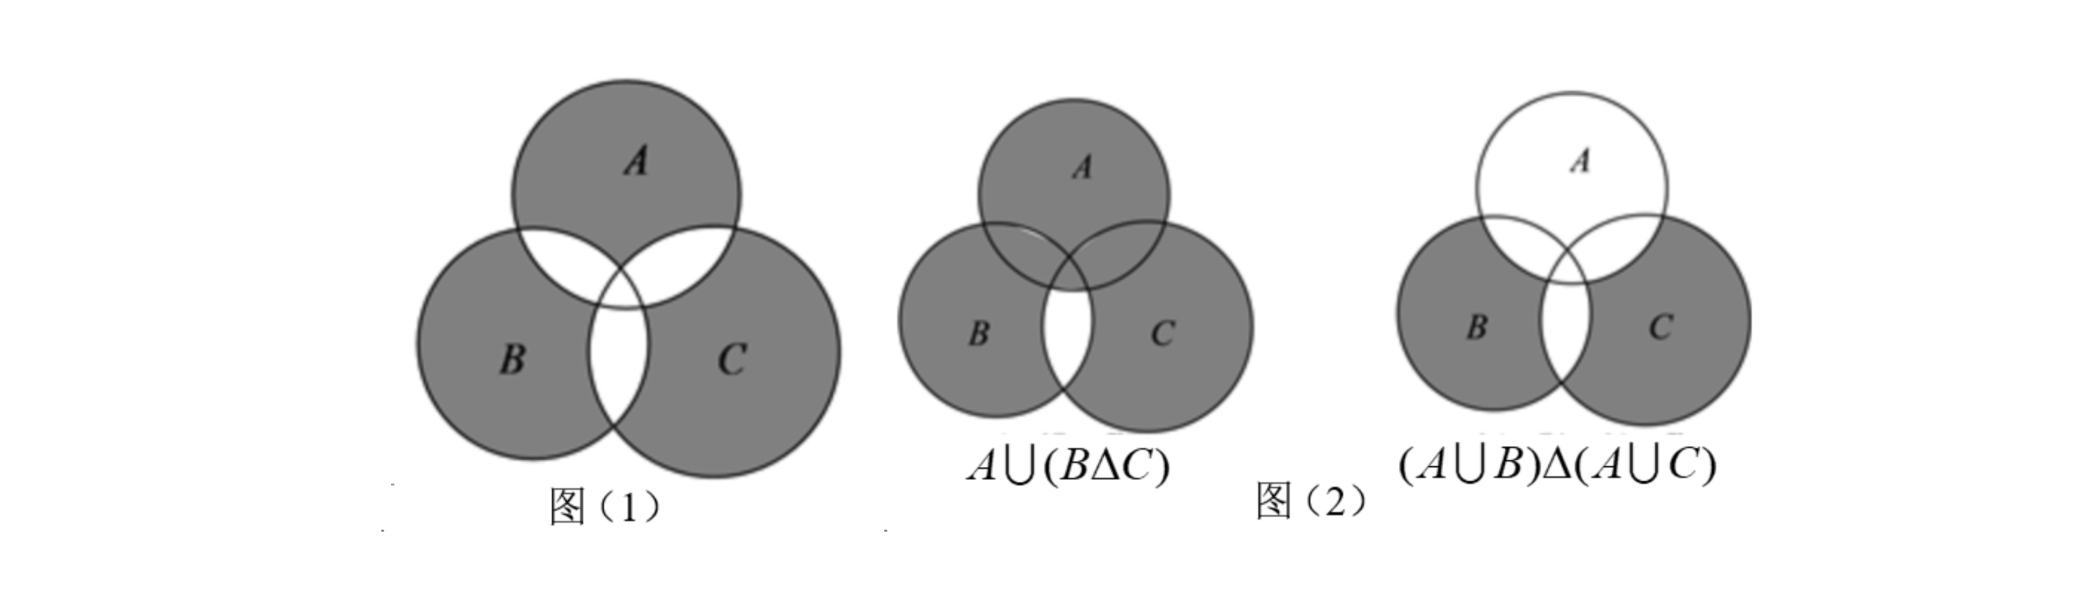
\includegraphics[width=0.92\textwidth]{figures/gao73_q16_symdiff.png}
\end{center}
\step{故选 $B$.}
\solend
\fi

\end{enumerate}

\bigsec{三、解答题}

\begin{enumerate}
\setcounter{enumi}{16}

\item （1）解不等式 $\dfrac{2-x}{x+3}>1$；

（2）已知 $a$ 是实数，试解关于 $x$ 的不等式：$x^2+(a-1)x-a\geqslant0$.

\ifanswer
\solbegin
\stepm{(1)}{$\dfrac{2-x}{x+3}-1=\dfrac{-2x-1}{x+3}>0$，则 $(2x+1)(x+3)<0$，得 $-3<x<-\dfrac12$，}
\step{所以不等式解集为 $\left(-3,-\dfrac12\right)$；}
\stepm{(2)}{$x^2+(a-1)x-a=(x+a)(x-1)\geqslant0$，}
% 原卷 (2) 题干为 ≥0，但解析按 ≤0 给出“两根之间”的解集，照录（见文件头“原卷笔误/存疑”②）
\step{当 $-a<1$，即 $a>-1$ 时，解集为 $(-a,1)$；}
\step{当 $-a=1$，即 $a=-1$ 时，解集为 $\R$；}
\step{当 $-a>1$，即 $a<-1$ 时，解集为 $(1,-a)$；}
\step{综上，当 $a>-1$ 时，解集为 $(-a,1)$；}
\step{当 $a=-1$ 时，解集为 $\R$；}
\step{当 $a<-1$ 时，解集为 $(1,-a)$.}
\solend
\fi

\ansspace[5]

\item （1）设 $a$、$b$ 是两个正数. 已知 $a>b$，比较 $\dfrac{2a+b}{a+2b}$ 与 $\dfrac ab$ 的值的大小；

（2）若实数 $a$ 满足 $\sqrt{(2023-a)^2}+\sqrt{a-2024}=a$，求 $a-2023^2$ 的值.

\ifanswer
\solbegin
\stepm{(1)}{$\dfrac{2a+b}{a+2b}-\dfrac ab=\dfrac{b^2-a^2}{b(a+2b)}<0$，所以 $\dfrac{2a+b}{a+2b}<\dfrac ab$.}
\stepm{(2)}{因为 $a-2024\geqslant0$，所以 $a\geqslant2024$，}
\step{所以 $\sqrt{(2023-a)^2}+\sqrt{a-2024}=a-2023+\sqrt{a-2024}$，}
\step{即 $a-2023+\sqrt{a-2024}=a$，即 $\sqrt{a-2024}=2023$，}
\step{所以 $a-2024=2023^2$，所以 $a-2023^2=2024$.}
\solend
\fi

\ansspace[5]

\item 已知 $m\in\R$，集合 $A=\{x\mid-1\leqslant x\leqslant3\}$，$B=\{x\mid m-3<x\leqslant m+2\}$.

（1）若“$x\in A$”是“$x\in B$”的充分不必要条件，求 $m$ 的取值范围；

（2）若 $A\cap B\neq\varnothing$，求 $m$ 的取值范围.

\ifanswer
\solbegin
\stepm{(1)}{因为“$x\in A$”是“$x\in B$”的充分不必要条件，所以 $A$ 是 $B$ 的真子集，}
\step{需满足 $\begin{cases}m-3<-1\\ m+2\geqslant3\end{cases}$，解得 $\begin{cases}m<2\\ m\geqslant1\end{cases}$，所以 $m$ 的取值范围是 $[1,2)$.}
\stepm{(2)}{因为 $A\cap B\neq\varnothing$，所以 $\begin{cases}m+2\geqslant-1\\ m-3<3\end{cases}$，解得 $\begin{cases}m\geqslant-3\\ m<6\end{cases}$，}
\step{所以 $m$ 的取值范围是 $[-3,6)$.}
\solend
\fi

\ansspace[6]

\item 已知集合 $A=\{x\mid x<-2\text{ 或 }x\geqslant3\}$，$U=\R$.

（1）若 $B=\{x\mid mx-1>0\}$，当 $B\subseteq A$ 时，求实数 $m$ 的取值范围；

（2）若 $B=\{x\mid2m-6\leqslant x\leqslant m+4\}$，当 $B\cap\overline A=\varnothing$ 时，求实数 $m$ 的取值范围.

\ifanswer
\solbegin
\stepm{(1)}{当 $m=0$ 时，$B=\varnothing$，符合题意，}
\step{当 $m>0$ 时，$B=\left\{x\mid x>\dfrac1m\right\}$，则 $\dfrac1m\geqslant3$，解得 $0<m\leqslant\dfrac13$，}
\step{当 $m<0$ 时，$B=\left\{x\mid x<\dfrac1m\right\}$，则 $\dfrac1m\leqslant-2$，解得 $-\dfrac12\leqslant m<0$，}
\step{综上所述，实数 $m$ 的取值范围 $\left[-\dfrac12,\dfrac13\right]$；}
\stepm{(2)}{由题意得 $B=\{x\mid2m-6\leqslant x\leqslant m+4\}$，$\overline A=\{x\mid-2\leqslant x<3\}$，且 $B\cap\overline A=\varnothing$，}
\step{当 $B=\varnothing$ 时，$2m-6>m+4$，解得 $m>10$，}
\step{当 $B\neq\varnothing$ 时，$\begin{cases}2m-6\leqslant m+4\\ m+4<-2\end{cases}$ 或 $\begin{cases}2m-6\leqslant m+4\\ 2m-6\geqslant3\end{cases}$，解得 $m<-6$ 或 $\dfrac92\leqslant m\leqslant10$，}
\step{综上所述，实数 $m$ 的取值范围为 $(-\infty,-6)\cup\left[\dfrac92,+\infty\right)$.}
\solend
\fi

\ansspace[7]

\item 关于实数大小关系的基本事实是解决等式或不等式问题的逻辑基础. 两个正数的大小关系是完全确定的，但通过运算就会产生非常奇妙的变化，基本不等式就是其中之一. 通过运算（代数变形）可以解决很多关于基本不等式的问题.

例如此题：正实数 $x$、$y$，满足 $x+y=1$，求 $\dfrac1x+\dfrac4y$ 的最小值. 求解本问题的方法很多，其中一种求解方法是：$\dfrac1x+\dfrac4y=(x+y)\left(\dfrac1x+\dfrac4y\right)=5+\dfrac yx+\dfrac{4x}{y}\geqslant5+2\sqrt{\dfrac yx\cdot\dfrac{4x}{y}}=9$，当且仅当 $\dfrac yx=\dfrac{4x}{y}$ 即 $y=2x$ 且 $x+y=1$ 时，即 $x=\dfrac13$，$y=\dfrac23$ 时等号成立.

这种解题方法叫作“$1$”的代换，利用上述求解方法解决下列问题：

（1）正数 $a$、$b$ 满足 $a+b=1$，求 $\dfrac1a+\dfrac2b$ 的最小值；

（2）已知 $a$、$b$、$c$ 均为正实数，且 $\dfrac1a+\dfrac1b+\dfrac1c=1$，求证：$a+b+c\geqslant9$；

（3）已知 $a$、$b$、$x$、$y$ 均为正实数，且 $\dfrac{x^2}{a^2}-\dfrac{y^2}{b^2}=1$，求证：$a^2-b^2\leqslant(x-y)^2$.

\ifanswer
\solbegin
\stepm{(1)}{正数 $a$、$b$ 满足 $a+b=1$，}
\step{$\dfrac1a+\dfrac2b=(a+b)\left(\dfrac1a+\dfrac2b\right)=1+2+\dfrac ba+\dfrac{2a}{b}\geqslant3+2\sqrt{\dfrac ba\cdot\dfrac{2a}{b}}=3+2\sqrt2$，}
\step{当且仅当 $\dfrac ba=\dfrac{2a}{b}$ 即 $b=\sqrt2\,a$ 且 $a+b=1$ 时，}
\step{即 $a=\sqrt2-1$，$b=2-\sqrt2$ 时取等号.}
\stepm{(2)}{$a+b+c=\left(\dfrac1a+\dfrac1b+\dfrac1c\right)(a+b+c)=3+\dfrac ba+\dfrac ab+\dfrac ca+\dfrac ac+\dfrac cb+\dfrac bc$}
\step{$\geqslant3+2\sqrt{\dfrac ba\cdot\dfrac ab}+2\sqrt{\dfrac ca\cdot\dfrac ac}+2\sqrt{\dfrac cb\cdot\dfrac bc}=9$，当且仅当 $a=b=c=3$ 时取等号，}
\step{故 $a+b+c\geqslant9$.}
\stepm{(3)}{$a^2-b^2=(a^2-b^2)\left(\dfrac{x^2}{a^2}-\dfrac{y^2}{b^2}\right)=x^2+y^2-\dfrac{b^2x^2}{a^2}-\dfrac{a^2y^2}{b^2}$}
\step{$=x^2+y^2-\left(\dfrac{b^2x^2}{a^2}+\dfrac{a^2y^2}{b^2}\right)\leqslant x^2+y^2-2\cdot\dfrac{bx}{a}\cdot\dfrac{ay}{b}=x^2+y^2-2xy$}
\step{$=(x-y)^2$，当且仅当 $\dfrac{bx}{a}=\dfrac{ay}{b}$ 且 $\dfrac{x^2}{a^2}-\dfrac{y^2}{b^2}=1$ 时，}
\step{即 $x=\dfrac{a^2}{\sqrt{a^2-b^2}}$，$y=\dfrac{b^2}{\sqrt{a^2-b^2}}$，$a>b$ 时取等号，故 $a^2-b^2\leqslant(x-y)^2$.}
\solend
\fi

\ansspace*[7]

\end{enumerate}

\end{document}
"
%
% 原始材料：微信公众号“魔都数学加油站”文章，连载“27学年高一73”；
% 原文标题“27学年高一73——2026-2027年上海市徐汇中学高一上10月月考”；
% 原文链接：https://mp.weixin.qq.com/s/Pkk9tFr4qHS9BR_BPxvk6A。
% 页面标注发布时间 2026-10-21 20:41（上海）。
% 正文为 10 张 PNG 页（`原图/高一73_徐汇中学_10月月考/01..10.png`）：
% 第 1、4、6、9、10 页为 2560×3620，其余 5 页为 4762×6735，均按页序读取。
% 10 页全为试卷正文页（卷首标题在第 1 页页顶，卷末第 21 题 (3) 解析止于第 10 页），
% 无封面页、目录页、二维码或宣传页。粉色斜排“魔都数学加油站”为卷面水印，未录入。
%
% 卷首标题：照卷面印作“2026-2027 年徐汇中学高一上 10 月月考”（黑体加粗一行）。
% 原卷年份区间用半角连字符，本稿按全稿惯例排 en dash；原卷无副标题。
%
% 篇幅与题号：原卷自第 3 题起编号（第 1、2 题不在本卷内）。填空题 3—12（10 题）、
% 选择题 13—16（4 题）、解答题 17—21（5 题），共 19 题。本稿沿用原节与原题号，
% 只改排为全稿统一的大节样式。
%
% 讲评版：原卷第 3、4 题只印【答案】（“没有实数根”“真”），本稿只给 \ans{}；
% 其余 17 题均印【解析】，用 \solbegin…\solend。四道选择题的作答括号原卷即留空，
% 答案写在解析末句“故选 A／D／A／B”，照录在解析内，不另提 \ans{}。
%
% 副标题：原卷未印副标题。本稿按“知识模块”口径标作“集合与常用逻辑用语、不等式”：
% 19 题中集合与常用逻辑用语 9 题（第 3、4、7、11、12、13、16、19、20 题），
% 不等式 10 题（第 5、6、8、9、10、14、15、17、18、21 题），两类均确有分量，故并标。
% 口径同 高一63、高一68—72。
%
% 与原卷的排版差异：
%   ① 原卷每题下直接印【答案】/【解析】，本稿按全稿惯例将答案与解析置于答案版；
%   ② 原卷未印副标题，本稿按“知识模块”口径补出；
%   ③ 原卷填空横线约四个字宽，本稿按全稿惯例统一排 \blankline[4.4em]；
%   ④ 原卷数集记号排斜体 $R$（第 3、8、9、10、12、17、19、20 题等），本稿按全稿惯例
%      改用 $\R$（同 高一68—72）；空集记号原卷作 $\varnothing$，照录；
%   ⑤ 原卷句末标点多为西文句点，第 15 题题干“整数解只有 $-2$”后为全角逗号，
%      均逐处照录；第 16 题解析的集合运算用 $\Delta$ 表示对称差，照原卷符号排；
%   ⑥ 第 17—21 题的子问原卷印作“（1）…（2）…”，本稿按 高一69—72 成例用行内
%      “（1）（2）（3）”段，解析中的子问标号用 \stepm{(1)}{…}；
%   ⑦ 每道解答题原卷未留作答空白，本稿按全稿惯例加 \ansspace（末题用 \ansspace*）；
%   ⑧ 选择题的作答括号原卷排半角“(    )”，本稿按全稿惯例排 \mbox{（\quad）}；
%      选项行排照原卷——第 13 题一行四条、第 14—16 题一行四条；
%   ⑨ 第 15 题题干的不等式组、第 14、19、20 题解析中的不等式组，原卷均排作“{”
%      连接的多行式，本稿按全稿惯例排 cases；
%   ⑩ 第 16 题解析末尾有三幅韦恩图（图（1）与图（2）的两幅）：原卷印在【解析】中，
%      题干无“如图”二字。本稿按原卷截图裁取（`figures/gao73_q16_symdiff.png`，
%      由第 6 页原图裁出、去除粉色水印后转灰度，未放大），放在答案版解析④之后。
%
% 原卷笔误/存疑（均照录未改，正文对应处另有 % 注）：
%   ① 第 3 题题干“设 $a$、$b\in\R$，则方程 $x^2+ax+a-1=0$ 至少有一个实根”中
%      $b$ 未在方程或后文出现，疑为衍字；原卷如此，照录未改。
%   ② 第 17 题 (2) 题干为 $x^2+(a-1)x-a\geqslant0$，但解析按 $\leqslant0$ 给出解集：
%      $a>-1$ 时写 $(-a,1)$、$a<-1$ 时写 $(1,-a)$，恰是“两根之间”的区间。
%      按题干 $\geqslant0$ 应为 $(-\infty,-a]\cup[1,+\infty)$ 与 $(-\infty,1]\cup[-a,+\infty)$；
%      原卷如此，照录未改。
%
% 行数核对：逐题数 \step/\stepm 条数与原卷【解析】印刷行数，17 题逐一相符，
% 合计 104 条 / 104 行（Q5：1；Q6：2；Q7：4；Q8：4；Q9：3；Q10：4；Q11：8；
% Q12：7；Q13：7；Q14：5；Q15：7；Q16：15；Q17：9；Q18：5；Q19：4；Q20：8；Q21：11）。
% 另第 3、4 题只印【答案】，各提 \ans{}，不计入 \step 账。
%
% 插图：第 16 题解析末的 3 幅韦恩图，见上⑩；全卷题干无其他配图。
%
\documentclass[a4paper,11pt]{article}
\usepackage{common}

\begin{document}

\examtitlest[3]{2026--2027 年徐汇中学高一上 10 月月考}{集合与常用逻辑用语、不等式}

\bigsec{一、填空题}

\begin{enumerate}
\setcounter{enumi}{2}

% 原卷题干“设 a、b∈R”中的 b 未在方程中出现，照录（见文件头“原卷笔误/存疑”①）
\item 如果用反证法证明命题“设 $a$、$b\in\R$，则方程 $x^2+ax+a-1=0$ 至少有一个实根”，那么首先假设方程 $x^2+ax+a-1=0$\blankline[4.4em].

\ifanswer
\ans{没有实数根}
\fi

\item 命题“若 $\dfrac1x>1$，则 $x<1$”是\blankline[4.4em]命题（填“真”，“假”）.

\ifanswer
\ans{真}
\fi

\item 对数 $\log_a(5-a)$ 中实数 $a$ 的取值范围是\blankline[4.4em].

\ifanswer
\solbegin
\step{由对数定义得 $\begin{cases}a>0\\ a\neq1\\ 5-a>0\end{cases}$，解得 $0<a<1$ 或 $1<a<5$.}
\solend
\fi

\item 关于 $x$ 的不等式 $ax^2-(a+1)x+1\leqslant0\,(a<0)$ 的解集为\blankline[4.4em].

\ifanswer
\solbegin
\step{原不等式即 $(ax-1)(x-1)\leqslant0$，因为 $a<0$，所以 $\left(x-\dfrac1a\right)(x-1)\geqslant0$.}
\step{又 $\dfrac1a<0<1$，所以 $x\leqslant\dfrac1a$ 或 $x\geqslant1$，故解集为 $\left(-\infty,\dfrac1a\right]\cup[1,+\infty)$.}
\solend
\fi

\item 若集合 $A=\{x\mid x^2-2kx+7k=0\}$ 有且仅有三个真子集，则 $k$ 的取值范围是\blankline[4.4em].

\ifanswer
\solbegin
\step{因为集合 $A$ 有且仅有三个真子集，则 $2^n-1=3$，解得 $n=2$，}
\step{所以一元二次方程 $x^2-2kx+7k=0$ 有两个不同的实数解，}
\step{则 $\Delta=4k^2-28k>0$，解得 $k<0$ 或 $k>7$，}
\step{故 $k$ 的取值范围是 $(-\infty,0)\cup(7,+\infty)$.}
\solend
\fi

\item 已知关于 $x$ 的不等式 $kx^2-4kx+k-6<0$ 对任意 $x\in\R$ 恒成立，则 $k$ 的取值范围是\blankline[4.4em].

\ifanswer
\solbegin
\step{关于 $x$ 的不等式 $kx^2-4kx+k-6<0$ 对任意 $x\in\R$ 恒成立，}
\step{当 $k=0$ 时，$kx^2-4kx+k-6=-6<0$ 恒成立，}
\step{当 $k\neq0$ 时，则 $\begin{cases}\Delta=16k^2-4k(k-6)<0\\ k<0\end{cases}$，解得 $-2<k<0$，}
\step{综上，$k$ 的取值范围为 $(-2,0]$.}
\solend
\fi

\item 设 $x\in\R$，方程 $|x-1|+|2x-1|=|3x-2|$ 的解集为\blankline[4.4em].

\ifanswer
\solbegin
\step{因为 $|x-1|+|2x-1|\geqslant|(x-1)+(2x-1)|=|3x-2|$，}
\step{当且仅当 $(x-1)(2x-1)\geqslant0$，解得 $x\leqslant\dfrac12$ 或 $x\geqslant1$，}
\step{故方程 $|x-1|+|2x-1|=|3x-2|$ 的解集为 $\left(-\infty,\dfrac12\right]\cup[1,+\infty)$.}
\solend
\fi

\item 已知 $a\in\R$，若关于 $x$ 的方程 $x^2+ax+a^2-8=0$ 有两个实根 $x_1$、$x_2$，且 $\dfrac1{x_1}+\dfrac1{x_2}=-\dfrac12$，则 $a$ 的值为\blankline[4.4em].

\ifanswer
\solbegin
\step{由题意得 $\Delta=a^2-4(a^2-8)=32-3a^2\geqslant0$，解得 $a^2\leqslant\dfrac{32}3$，}
\step{由韦达定理得 $x_1+x_2=-a$，$x_1x_2=a^2-8$，}
\step{则 $\dfrac1{x_1}+\dfrac1{x_2}=\dfrac{x_1+x_2}{x_1x_2}=\dfrac{-a}{a^2-8}=-\dfrac12$，即 $a^2-2a-8=(a-4)(a+2)=0$，}
\step{解得 $a=4$ 或 $a=-2$. 又 $a^2\leqslant\dfrac{32}3$，则 $a=-2$.}
\solend
\fi

\item 甲、乙两人解关于 $x$ 的不等式 $x^2+bx+c<0$，甲写错了 $b$，正确计算后得到的解为 $\{x\mid1<x<2\}$；乙写错了 $c$，正确计算后得到的解为 $\{x\mid-4<x<1\}$. 那么不等式 $\dfrac{bx+c}{x-2}<0$ 的解为\blankline[4.4em].

\ifanswer
\solbegin
\step{由 $x^2+bx+c<0$ 的解为 $\{x\mid1<x<2\}$，}
\step{则 $1$ 和 $2$ 是方程 $x^2+bx+c=0$ 的两个根，}
\step{甲写错了 $b$，但 $c$ 是正确的，所以 $c=1\times2=2$；}
\step{由 $x^2+bx+c<0$ 的解为 $\{x\mid-4<x<1\}$，}
\step{则 $-4$ 和 $1$ 是方程 $x^2+bx+c=0$ 的两个根，}
\step{乙写错了 $c$，但 $b$ 是正确的，所以 $-b=-4+1=-3$，即 $b=3$.}
\step{由 $\dfrac{bx+c}{x-2}<0$，得 $\dfrac{3x+2}{x-2}<0$，即 $(3x+2)(x-2)<0$，解得 $-\dfrac23<x<2$，}
\step{所以不等式 $\dfrac{bx+c}{x-2}<0$ 的解为 $\left\{x\mid-\dfrac23<x<2\right\}$.}
\solend
\fi

\item 设 $a,b,c\in\R$，$S=\{x\mid(x+a)(x^2+bx+c)=0,x\in\R\}$，$T=\{x\mid(ax+1)(cx^2+bx+1)=0,x\in\R\}$. 若 $|S|$、$|T|$ 分别为集合 $S$、$T$ 的元素个数，则 $|S|+|T|$ 的所有可能取值组成的集合为\blankline[4.4em].

\ifanswer
\solbegin
\step{$x\neq0$ 时，$(ax+1)(cx^2+bx+1)=x^3\left(\dfrac1x+a\right)\left(\dfrac1{x^2}+\dfrac bx+c\right)$，}
\step{故 $S$、$T$ 的非零元按倒数一一对应，设其个数均为 $k$；}
\step{$0\notin T$，且 $0\in S\Leftrightarrow ac=0$. 当 $ac=0$ 时 $k\in\{0,1,2\}$，}
\step{当 $ac\neq0$ 时 $x=-a\neq0$ 是 $S$ 的非零元，$k\in\{1,2,3\}$.}
\step{因此 $|S|+|T|$ 分别可取 $2k+1\in\{1,3,5\}$ 与 $2k\in\{2,4,6\}$.}
\step{依次取 $(a,b,c)=(0,0,0),(1,0,1),(0,-2,1),(1,-2,1),(0,0,-1),(1,-5,6)$，可分别实现 $1,2,3,4,5,6$，}
\step{则 $|S|+|T|$ 的所有可能取值组成的集合为 $\{1,2,3,4,5,6\}$.}
\solend
\fi

\end{enumerate}

\bigsec{二、选择题}

\begin{enumerate}
\setcounter{enumi}{12}

\item 如果 $a>b$，$c\neq0$，那么下列不等式成立的是\mbox{（\quad）}

\keepwithprev
A. $a-c>b-c$\qquad B. $c-a>c-b$\qquad C. $ac>bc$\qquad D. $\dfrac ac>\dfrac bc$

\ifanswer
\solbegin
\step{对于 $A$：$a-c-(b-c)=a-b>0$，即 $a-c>b-c$，故 $A$ 正确；}
\step{对于 $B$：$c-a-(c-b)=b-a<0$，即 $c-a<c-b$，故 $B$ 错误；}
\step{对于 $C$：$ac-bc=c(a-b)$，已知 $a-b>0$，}
\step{当 $c<0$ 时，$c(a-b)<0$，此时 $ac<bc$，故 $C$ 错误；}
\step{对于 $D$：$\dfrac ac-\dfrac bc=\dfrac1c(a-b)$，已知 $a-b>0$，}
\step{当 $c<0$ 时，$\dfrac1c(a-b)<0$，此时 $\dfrac ac<\dfrac bc$，故 $D$ 错误.}
\step{故选 $A$.}
\solend
\fi

\item 若不等式 $|x+1|\leqslant a$ 成立的一个充分不必要条件是 $-3\leqslant x\leqslant4$，则整数 $a$ 的最小值为\mbox{（\quad）}

\keepwithprev
A. $2$\qquad B. $3$\qquad C. $4$\qquad D. $5$

\ifanswer
\solbegin
\step{若 $a<0$，则 $|x+1|\leqslant a$ 无解；}
\step{若 $a\geqslant0$，由 $|x+1|\leqslant a$，得 $-1-a\leqslant x\leqslant-1+a$，}
\step{因为 $|x+1|\leqslant a$ 成立的一个充分不必要条件是 $-3\leqslant x\leqslant4$，}
\step{所以 $\begin{cases}-1-a\leqslant-3\\ -1+a\geqslant4\end{cases}$，等号不同时成立，解得 $a\geqslant5$，}
\step{故整数 $a$ 的最小值为 $5$. 故选 $D$.}
\solend
\fi

\item 若关于 $x$ 的不等式组 $\begin{cases}x^2-x-2>0\\ 2x^2+(5+2k)x+5k<0\end{cases}$ 的整数解只有 $-2$，则实数 $k$ 的取值范围为\mbox{（\quad）}

\keepwithprev
A. $[-3,2)$\qquad B. $[1,2]$\qquad C. $(1,2]$\qquad D. $(1,2)$

\ifanswer
\solbegin
\step{由 $x^2-x-2>0$，得 $x>2$ 或 $x<-1$，}
\step{由 $2x^2+(2k+5)x+5k<0$，得 $(2x+5)(x+k)<0$.}
\step{①若 $-k<-\dfrac52$，即 $k>\dfrac52$ 时，解得 $-k<x<-\dfrac52$，}
\step{此时原不等式的解集为 $\left(-k,-\dfrac52\right)$，不符合题意；}
\step{②若 $k=\dfrac52$ 时，解得 $x\in\varnothing$，显然不符合题意；}
\step{③若 $k<\dfrac52$ 时，解得 $-\dfrac52<x<-k$，则 $-2<-k\leqslant3$，即 $-3\leqslant k<2$.}
\step{综上，实数 $k$ 的取值范围 $[-3,2)$. 故选 $A$.}
\solend
\fi

\item 定义集合运算 $A-B=\{x\mid x\in A\text{ 且 }x\notin B\}$ 称为集合 $A$ 与集合 $B$ 的差集；定义集合运算 $A\Delta B=(A-B)\cup(B-A)$ 称为集合 $A$ 与集合 $B$ 的对称差，有以下 $4$ 个等式：

① $A\Delta B=B\Delta A$；

② $(A\Delta B)\Delta C=A\Delta(B\Delta C)$；

③ $A\cap(B\Delta C)=(A\cap B)\Delta(A\cap C)$；

④ $A\cup(B\Delta C)=(A\cup B)\Delta(A\cup C)$.

则 $4$ 个等式中恒成立的是\mbox{（\quad）}

\keepwithprev
A. ①②\qquad B. ①②③\qquad C. ①②④\qquad D. ①②③④

\ifanswer
\solbegin
\step{对于①，由 $B\Delta A=(B-A)\cup(A-B)=(A-B)\cup(B-A)=A\Delta B$，}
\step{所以①正确；}
\step{对于②，}
\step{由 $A-B=\{x\mid x\in A\text{ 且 }x\notin B\}=\{x\mid x\in A,x\notin(A\cap B)\}=A-(A\cap B)$，}
\step{同理可得 $B-A=B-(A\cap B)$，}
\step{则 $A\Delta B=(A-B)\cup(B-A)=(A\cup B)-(A\cap B)$，}
\step{所以 $(A\Delta B)\Delta C=(A\Delta B)\cup C-(A\Delta B)\cap C$，}
\step{所以表示的集合为图（1）中阴影部分所表示的集合，如图所示，}
\step{同理 $A\Delta(B\Delta C)=A\cup(B\Delta C)-A\cap(B\Delta C)$，}
\step{也表示图（1）中阴影部分所表示的集合，}
\step{所以 $(A\Delta B)\Delta C=A\Delta(B\Delta C)$，所以②正确；}
\step{对于③，由 $A\cap(B\Delta C)=A\cap(B\cup C-B\cap C)=A\cap(B\cup C)-A\cap(B\cap C)$}
\step{$=(A\cap B)\cup(A\cap C)-(A\cap B)\cap(A\cap C)=(A\cap B)\Delta(A\cap C)$，所以③正确；}
\step{对于④，如图（2）所示，$A\cup(B\Delta C)\neq(A\cup B)\Delta(A\cup C)$，所以④错误.}
\begin{center}
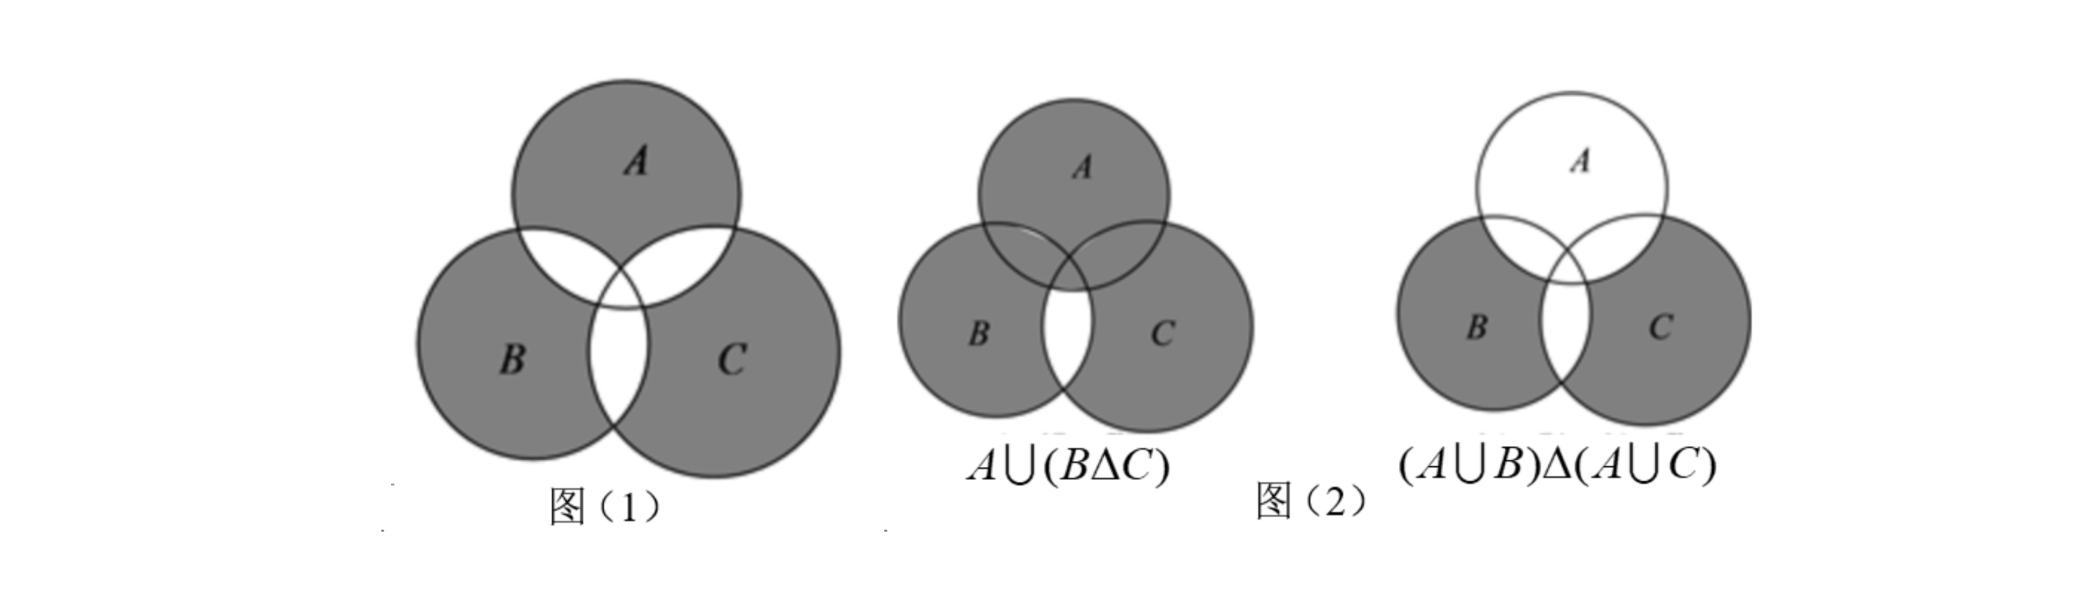
\includegraphics[width=0.92\textwidth]{figures/gao73_q16_symdiff.png}
\end{center}
\step{故选 $B$.}
\solend
\fi

\end{enumerate}

\bigsec{三、解答题}

\begin{enumerate}
\setcounter{enumi}{16}

\item （1）解不等式 $\dfrac{2-x}{x+3}>1$；

（2）已知 $a$ 是实数，试解关于 $x$ 的不等式：$x^2+(a-1)x-a\geqslant0$.

\ifanswer
\solbegin
\stepm{(1)}{$\dfrac{2-x}{x+3}-1=\dfrac{-2x-1}{x+3}>0$，则 $(2x+1)(x+3)<0$，得 $-3<x<-\dfrac12$，}
\step{所以不等式解集为 $\left(-3,-\dfrac12\right)$；}
\stepm{(2)}{$x^2+(a-1)x-a=(x+a)(x-1)\geqslant0$，}
% 原卷 (2) 题干为 ≥0，但解析按 ≤0 给出“两根之间”的解集，照录（见文件头“原卷笔误/存疑”②）
\step{当 $-a<1$，即 $a>-1$ 时，解集为 $(-a,1)$；}
\step{当 $-a=1$，即 $a=-1$ 时，解集为 $\R$；}
\step{当 $-a>1$，即 $a<-1$ 时，解集为 $(1,-a)$；}
\step{综上，当 $a>-1$ 时，解集为 $(-a,1)$；}
\step{当 $a=-1$ 时，解集为 $\R$；}
\step{当 $a<-1$ 时，解集为 $(1,-a)$.}
\solend
\fi

\ansspace[5]

\item （1）设 $a$、$b$ 是两个正数. 已知 $a>b$，比较 $\dfrac{2a+b}{a+2b}$ 与 $\dfrac ab$ 的值的大小；

（2）若实数 $a$ 满足 $\sqrt{(2023-a)^2}+\sqrt{a-2024}=a$，求 $a-2023^2$ 的值.

\ifanswer
\solbegin
\stepm{(1)}{$\dfrac{2a+b}{a+2b}-\dfrac ab=\dfrac{b^2-a^2}{b(a+2b)}<0$，所以 $\dfrac{2a+b}{a+2b}<\dfrac ab$.}
\stepm{(2)}{因为 $a-2024\geqslant0$，所以 $a\geqslant2024$，}
\step{所以 $\sqrt{(2023-a)^2}+\sqrt{a-2024}=a-2023+\sqrt{a-2024}$，}
\step{即 $a-2023+\sqrt{a-2024}=a$，即 $\sqrt{a-2024}=2023$，}
\step{所以 $a-2024=2023^2$，所以 $a-2023^2=2024$.}
\solend
\fi

\ansspace[5]

\item 已知 $m\in\R$，集合 $A=\{x\mid-1\leqslant x\leqslant3\}$，$B=\{x\mid m-3<x\leqslant m+2\}$.

（1）若“$x\in A$”是“$x\in B$”的充分不必要条件，求 $m$ 的取值范围；

（2）若 $A\cap B\neq\varnothing$，求 $m$ 的取值范围.

\ifanswer
\solbegin
\stepm{(1)}{因为“$x\in A$”是“$x\in B$”的充分不必要条件，所以 $A$ 是 $B$ 的真子集，}
\step{需满足 $\begin{cases}m-3<-1\\ m+2\geqslant3\end{cases}$，解得 $\begin{cases}m<2\\ m\geqslant1\end{cases}$，所以 $m$ 的取值范围是 $[1,2)$.}
\stepm{(2)}{因为 $A\cap B\neq\varnothing$，所以 $\begin{cases}m+2\geqslant-1\\ m-3<3\end{cases}$，解得 $\begin{cases}m\geqslant-3\\ m<6\end{cases}$，}
\step{所以 $m$ 的取值范围是 $[-3,6)$.}
\solend
\fi

\ansspace[6]

\item 已知集合 $A=\{x\mid x<-2\text{ 或 }x\geqslant3\}$，$U=\R$.

（1）若 $B=\{x\mid mx-1>0\}$，当 $B\subseteq A$ 时，求实数 $m$ 的取值范围；

（2）若 $B=\{x\mid2m-6\leqslant x\leqslant m+4\}$，当 $B\cap\overline A=\varnothing$ 时，求实数 $m$ 的取值范围.

\ifanswer
\solbegin
\stepm{(1)}{当 $m=0$ 时，$B=\varnothing$，符合题意，}
\step{当 $m>0$ 时，$B=\left\{x\mid x>\dfrac1m\right\}$，则 $\dfrac1m\geqslant3$，解得 $0<m\leqslant\dfrac13$，}
\step{当 $m<0$ 时，$B=\left\{x\mid x<\dfrac1m\right\}$，则 $\dfrac1m\leqslant-2$，解得 $-\dfrac12\leqslant m<0$，}
\step{综上所述，实数 $m$ 的取值范围 $\left[-\dfrac12,\dfrac13\right]$；}
\stepm{(2)}{由题意得 $B=\{x\mid2m-6\leqslant x\leqslant m+4\}$，$\overline A=\{x\mid-2\leqslant x<3\}$，且 $B\cap\overline A=\varnothing$，}
\step{当 $B=\varnothing$ 时，$2m-6>m+4$，解得 $m>10$，}
\step{当 $B\neq\varnothing$ 时，$\begin{cases}2m-6\leqslant m+4\\ m+4<-2\end{cases}$ 或 $\begin{cases}2m-6\leqslant m+4\\ 2m-6\geqslant3\end{cases}$，解得 $m<-6$ 或 $\dfrac92\leqslant m\leqslant10$，}
\step{综上所述，实数 $m$ 的取值范围为 $(-\infty,-6)\cup\left[\dfrac92,+\infty\right)$.}
\solend
\fi

\ansspace[7]

\item 关于实数大小关系的基本事实是解决等式或不等式问题的逻辑基础. 两个正数的大小关系是完全确定的，但通过运算就会产生非常奇妙的变化，基本不等式就是其中之一. 通过运算（代数变形）可以解决很多关于基本不等式的问题.

例如此题：正实数 $x$、$y$，满足 $x+y=1$，求 $\dfrac1x+\dfrac4y$ 的最小值. 求解本问题的方法很多，其中一种求解方法是：$\dfrac1x+\dfrac4y=(x+y)\left(\dfrac1x+\dfrac4y\right)=5+\dfrac yx+\dfrac{4x}{y}\geqslant5+2\sqrt{\dfrac yx\cdot\dfrac{4x}{y}}=9$，当且仅当 $\dfrac yx=\dfrac{4x}{y}$ 即 $y=2x$ 且 $x+y=1$ 时，即 $x=\dfrac13$，$y=\dfrac23$ 时等号成立.

这种解题方法叫作“$1$”的代换，利用上述求解方法解决下列问题：

（1）正数 $a$、$b$ 满足 $a+b=1$，求 $\dfrac1a+\dfrac2b$ 的最小值；

（2）已知 $a$、$b$、$c$ 均为正实数，且 $\dfrac1a+\dfrac1b+\dfrac1c=1$，求证：$a+b+c\geqslant9$；

（3）已知 $a$、$b$、$x$、$y$ 均为正实数，且 $\dfrac{x^2}{a^2}-\dfrac{y^2}{b^2}=1$，求证：$a^2-b^2\leqslant(x-y)^2$.

\ifanswer
\solbegin
\stepm{(1)}{正数 $a$、$b$ 满足 $a+b=1$，}
\step{$\dfrac1a+\dfrac2b=(a+b)\left(\dfrac1a+\dfrac2b\right)=1+2+\dfrac ba+\dfrac{2a}{b}\geqslant3+2\sqrt{\dfrac ba\cdot\dfrac{2a}{b}}=3+2\sqrt2$，}
\step{当且仅当 $\dfrac ba=\dfrac{2a}{b}$ 即 $b=\sqrt2\,a$ 且 $a+b=1$ 时，}
\step{即 $a=\sqrt2-1$，$b=2-\sqrt2$ 时取等号.}
\stepm{(2)}{$a+b+c=\left(\dfrac1a+\dfrac1b+\dfrac1c\right)(a+b+c)=3+\dfrac ba+\dfrac ab+\dfrac ca+\dfrac ac+\dfrac cb+\dfrac bc$}
\step{$\geqslant3+2\sqrt{\dfrac ba\cdot\dfrac ab}+2\sqrt{\dfrac ca\cdot\dfrac ac}+2\sqrt{\dfrac cb\cdot\dfrac bc}=9$，当且仅当 $a=b=c=3$ 时取等号，}
\step{故 $a+b+c\geqslant9$.}
\stepm{(3)}{$a^2-b^2=(a^2-b^2)\left(\dfrac{x^2}{a^2}-\dfrac{y^2}{b^2}\right)=x^2+y^2-\dfrac{b^2x^2}{a^2}-\dfrac{a^2y^2}{b^2}$}
\step{$=x^2+y^2-\left(\dfrac{b^2x^2}{a^2}+\dfrac{a^2y^2}{b^2}\right)\leqslant x^2+y^2-2\cdot\dfrac{bx}{a}\cdot\dfrac{ay}{b}=x^2+y^2-2xy$}
\step{$=(x-y)^2$，当且仅当 $\dfrac{bx}{a}=\dfrac{ay}{b}$ 且 $\dfrac{x^2}{a^2}-\dfrac{y^2}{b^2}=1$ 时，}
\step{即 $x=\dfrac{a^2}{\sqrt{a^2-b^2}}$，$y=\dfrac{b^2}{\sqrt{a^2-b^2}}$，$a>b$ 时取等号，故 $a^2-b^2\leqslant(x-y)^2$.}
\solend
\fi

\ansspace*[7]

\end{enumerate}

\end{document}
"
% 紧凑版：xelatex "\def\iscompact{1}% 高一73_徐汇中学_10月月考.tex
%   —— 高一上数学“2026-2027 年徐汇中学高一上 10 月月考”（讲评版）
% 试卷版：xelatex 高一73_徐汇中学_10月月考.tex
% 答案版：xelatex "\def\isanswer{1}% 高一73_徐汇中学_10月月考.tex
%   —— 高一上数学“2026-2027 年徐汇中学高一上 10 月月考”（讲评版）
% 试卷版：xelatex 高一73_徐汇中学_10月月考.tex
% 答案版：xelatex "\def\isanswer{1}\input{高一73_徐汇中学_10月月考.tex}"
% 紧凑版：xelatex "\def\iscompact{1}\input{高一73_徐汇中学_10月月考.tex}"
%
% 原始材料：微信公众号“魔都数学加油站”文章，连载“27学年高一73”；
% 原文标题“27学年高一73——2026-2027年上海市徐汇中学高一上10月月考”；
% 原文链接：https://mp.weixin.qq.com/s/Pkk9tFr4qHS9BR_BPxvk6A。
% 页面标注发布时间 2026-10-21 20:41（上海）。
% 正文为 10 张 PNG 页（`原图/高一73_徐汇中学_10月月考/01..10.png`）：
% 第 1、4、6、9、10 页为 2560×3620，其余 5 页为 4762×6735，均按页序读取。
% 10 页全为试卷正文页（卷首标题在第 1 页页顶，卷末第 21 题 (3) 解析止于第 10 页），
% 无封面页、目录页、二维码或宣传页。粉色斜排“魔都数学加油站”为卷面水印，未录入。
%
% 卷首标题：照卷面印作“2026-2027 年徐汇中学高一上 10 月月考”（黑体加粗一行）。
% 原卷年份区间用半角连字符，本稿按全稿惯例排 en dash；原卷无副标题。
%
% 篇幅与题号：原卷自第 3 题起编号（第 1、2 题不在本卷内）。填空题 3—12（10 题）、
% 选择题 13—16（4 题）、解答题 17—21（5 题），共 19 题。本稿沿用原节与原题号，
% 只改排为全稿统一的大节样式。
%
% 讲评版：原卷第 3、4 题只印【答案】（“没有实数根”“真”），本稿只给 \ans{}；
% 其余 17 题均印【解析】，用 \solbegin…\solend。四道选择题的作答括号原卷即留空，
% 答案写在解析末句“故选 A／D／A／B”，照录在解析内，不另提 \ans{}。
%
% 副标题：原卷未印副标题。本稿按“知识模块”口径标作“集合与常用逻辑用语、不等式”：
% 19 题中集合与常用逻辑用语 9 题（第 3、4、7、11、12、13、16、19、20 题），
% 不等式 10 题（第 5、6、8、9、10、14、15、17、18、21 题），两类均确有分量，故并标。
% 口径同 高一63、高一68—72。
%
% 与原卷的排版差异：
%   ① 原卷每题下直接印【答案】/【解析】，本稿按全稿惯例将答案与解析置于答案版；
%   ② 原卷未印副标题，本稿按“知识模块”口径补出；
%   ③ 原卷填空横线约四个字宽，本稿按全稿惯例统一排 \blankline[4.4em]；
%   ④ 原卷数集记号排斜体 $R$（第 3、8、9、10、12、17、19、20 题等），本稿按全稿惯例
%      改用 $\R$（同 高一68—72）；空集记号原卷作 $\varnothing$，照录；
%   ⑤ 原卷句末标点多为西文句点，第 15 题题干“整数解只有 $-2$”后为全角逗号，
%      均逐处照录；第 16 题解析的集合运算用 $\Delta$ 表示对称差，照原卷符号排；
%   ⑥ 第 17—21 题的子问原卷印作“（1）…（2）…”，本稿按 高一69—72 成例用行内
%      “（1）（2）（3）”段，解析中的子问标号用 \stepm{(1)}{…}；
%   ⑦ 每道解答题原卷未留作答空白，本稿按全稿惯例加 \ansspace（末题用 \ansspace*）；
%   ⑧ 选择题的作答括号原卷排半角“(    )”，本稿按全稿惯例排 \mbox{（\quad）}；
%      选项行排照原卷——第 13 题一行四条、第 14—16 题一行四条；
%   ⑨ 第 15 题题干的不等式组、第 14、19、20 题解析中的不等式组，原卷均排作“{”
%      连接的多行式，本稿按全稿惯例排 cases；
%   ⑩ 第 16 题解析末尾有三幅韦恩图（图（1）与图（2）的两幅）：原卷印在【解析】中，
%      题干无“如图”二字。本稿按原卷截图裁取（`figures/gao73_q16_symdiff.png`，
%      由第 6 页原图裁出、去除粉色水印后转灰度，未放大），放在答案版解析④之后。
%
% 原卷笔误/存疑（均照录未改，正文对应处另有 % 注）：
%   ① 第 3 题题干“设 $a$、$b\in\R$，则方程 $x^2+ax+a-1=0$ 至少有一个实根”中
%      $b$ 未在方程或后文出现，疑为衍字；原卷如此，照录未改。
%   ② 第 17 题 (2) 题干为 $x^2+(a-1)x-a\geqslant0$，但解析按 $\leqslant0$ 给出解集：
%      $a>-1$ 时写 $(-a,1)$、$a<-1$ 时写 $(1,-a)$，恰是“两根之间”的区间。
%      按题干 $\geqslant0$ 应为 $(-\infty,-a]\cup[1,+\infty)$ 与 $(-\infty,1]\cup[-a,+\infty)$；
%      原卷如此，照录未改。
%
% 行数核对：逐题数 \step/\stepm 条数与原卷【解析】印刷行数，17 题逐一相符，
% 合计 104 条 / 104 行（Q5：1；Q6：2；Q7：4；Q8：4；Q9：3；Q10：4；Q11：8；
% Q12：7；Q13：7；Q14：5；Q15：7；Q16：15；Q17：9；Q18：5；Q19：4；Q20：8；Q21：11）。
% 另第 3、4 题只印【答案】，各提 \ans{}，不计入 \step 账。
%
% 插图：第 16 题解析末的 3 幅韦恩图，见上⑩；全卷题干无其他配图。
%
\documentclass[a4paper,11pt]{article}
\usepackage{common}

\begin{document}

\examtitlest[3]{2026--2027 年徐汇中学高一上 10 月月考}{集合与常用逻辑用语、不等式}

\bigsec{一、填空题}

\begin{enumerate}
\setcounter{enumi}{2}

% 原卷题干“设 a、b∈R”中的 b 未在方程中出现，照录（见文件头“原卷笔误/存疑”①）
\item 如果用反证法证明命题“设 $a$、$b\in\R$，则方程 $x^2+ax+a-1=0$ 至少有一个实根”，那么首先假设方程 $x^2+ax+a-1=0$\blankline[4.4em].

\ifanswer
\ans{没有实数根}
\fi

\item 命题“若 $\dfrac1x>1$，则 $x<1$”是\blankline[4.4em]命题（填“真”，“假”）.

\ifanswer
\ans{真}
\fi

\item 对数 $\log_a(5-a)$ 中实数 $a$ 的取值范围是\blankline[4.4em].

\ifanswer
\solbegin
\step{由对数定义得 $\begin{cases}a>0\\ a\neq1\\ 5-a>0\end{cases}$，解得 $0<a<1$ 或 $1<a<5$.}
\solend
\fi

\item 关于 $x$ 的不等式 $ax^2-(a+1)x+1\leqslant0\,(a<0)$ 的解集为\blankline[4.4em].

\ifanswer
\solbegin
\step{原不等式即 $(ax-1)(x-1)\leqslant0$，因为 $a<0$，所以 $\left(x-\dfrac1a\right)(x-1)\geqslant0$.}
\step{又 $\dfrac1a<0<1$，所以 $x\leqslant\dfrac1a$ 或 $x\geqslant1$，故解集为 $\left(-\infty,\dfrac1a\right]\cup[1,+\infty)$.}
\solend
\fi

\item 若集合 $A=\{x\mid x^2-2kx+7k=0\}$ 有且仅有三个真子集，则 $k$ 的取值范围是\blankline[4.4em].

\ifanswer
\solbegin
\step{因为集合 $A$ 有且仅有三个真子集，则 $2^n-1=3$，解得 $n=2$，}
\step{所以一元二次方程 $x^2-2kx+7k=0$ 有两个不同的实数解，}
\step{则 $\Delta=4k^2-28k>0$，解得 $k<0$ 或 $k>7$，}
\step{故 $k$ 的取值范围是 $(-\infty,0)\cup(7,+\infty)$.}
\solend
\fi

\item 已知关于 $x$ 的不等式 $kx^2-4kx+k-6<0$ 对任意 $x\in\R$ 恒成立，则 $k$ 的取值范围是\blankline[4.4em].

\ifanswer
\solbegin
\step{关于 $x$ 的不等式 $kx^2-4kx+k-6<0$ 对任意 $x\in\R$ 恒成立，}
\step{当 $k=0$ 时，$kx^2-4kx+k-6=-6<0$ 恒成立，}
\step{当 $k\neq0$ 时，则 $\begin{cases}\Delta=16k^2-4k(k-6)<0\\ k<0\end{cases}$，解得 $-2<k<0$，}
\step{综上，$k$ 的取值范围为 $(-2,0]$.}
\solend
\fi

\item 设 $x\in\R$，方程 $|x-1|+|2x-1|=|3x-2|$ 的解集为\blankline[4.4em].

\ifanswer
\solbegin
\step{因为 $|x-1|+|2x-1|\geqslant|(x-1)+(2x-1)|=|3x-2|$，}
\step{当且仅当 $(x-1)(2x-1)\geqslant0$，解得 $x\leqslant\dfrac12$ 或 $x\geqslant1$，}
\step{故方程 $|x-1|+|2x-1|=|3x-2|$ 的解集为 $\left(-\infty,\dfrac12\right]\cup[1,+\infty)$.}
\solend
\fi

\item 已知 $a\in\R$，若关于 $x$ 的方程 $x^2+ax+a^2-8=0$ 有两个实根 $x_1$、$x_2$，且 $\dfrac1{x_1}+\dfrac1{x_2}=-\dfrac12$，则 $a$ 的值为\blankline[4.4em].

\ifanswer
\solbegin
\step{由题意得 $\Delta=a^2-4(a^2-8)=32-3a^2\geqslant0$，解得 $a^2\leqslant\dfrac{32}3$，}
\step{由韦达定理得 $x_1+x_2=-a$，$x_1x_2=a^2-8$，}
\step{则 $\dfrac1{x_1}+\dfrac1{x_2}=\dfrac{x_1+x_2}{x_1x_2}=\dfrac{-a}{a^2-8}=-\dfrac12$，即 $a^2-2a-8=(a-4)(a+2)=0$，}
\step{解得 $a=4$ 或 $a=-2$. 又 $a^2\leqslant\dfrac{32}3$，则 $a=-2$.}
\solend
\fi

\item 甲、乙两人解关于 $x$ 的不等式 $x^2+bx+c<0$，甲写错了 $b$，正确计算后得到的解为 $\{x\mid1<x<2\}$；乙写错了 $c$，正确计算后得到的解为 $\{x\mid-4<x<1\}$. 那么不等式 $\dfrac{bx+c}{x-2}<0$ 的解为\blankline[4.4em].

\ifanswer
\solbegin
\step{由 $x^2+bx+c<0$ 的解为 $\{x\mid1<x<2\}$，}
\step{则 $1$ 和 $2$ 是方程 $x^2+bx+c=0$ 的两个根，}
\step{甲写错了 $b$，但 $c$ 是正确的，所以 $c=1\times2=2$；}
\step{由 $x^2+bx+c<0$ 的解为 $\{x\mid-4<x<1\}$，}
\step{则 $-4$ 和 $1$ 是方程 $x^2+bx+c=0$ 的两个根，}
\step{乙写错了 $c$，但 $b$ 是正确的，所以 $-b=-4+1=-3$，即 $b=3$.}
\step{由 $\dfrac{bx+c}{x-2}<0$，得 $\dfrac{3x+2}{x-2}<0$，即 $(3x+2)(x-2)<0$，解得 $-\dfrac23<x<2$，}
\step{所以不等式 $\dfrac{bx+c}{x-2}<0$ 的解为 $\left\{x\mid-\dfrac23<x<2\right\}$.}
\solend
\fi

\item 设 $a,b,c\in\R$，$S=\{x\mid(x+a)(x^2+bx+c)=0,x\in\R\}$，$T=\{x\mid(ax+1)(cx^2+bx+1)=0,x\in\R\}$. 若 $|S|$、$|T|$ 分别为集合 $S$、$T$ 的元素个数，则 $|S|+|T|$ 的所有可能取值组成的集合为\blankline[4.4em].

\ifanswer
\solbegin
\step{$x\neq0$ 时，$(ax+1)(cx^2+bx+1)=x^3\left(\dfrac1x+a\right)\left(\dfrac1{x^2}+\dfrac bx+c\right)$，}
\step{故 $S$、$T$ 的非零元按倒数一一对应，设其个数均为 $k$；}
\step{$0\notin T$，且 $0\in S\Leftrightarrow ac=0$. 当 $ac=0$ 时 $k\in\{0,1,2\}$，}
\step{当 $ac\neq0$ 时 $x=-a\neq0$ 是 $S$ 的非零元，$k\in\{1,2,3\}$.}
\step{因此 $|S|+|T|$ 分别可取 $2k+1\in\{1,3,5\}$ 与 $2k\in\{2,4,6\}$.}
\step{依次取 $(a,b,c)=(0,0,0),(1,0,1),(0,-2,1),(1,-2,1),(0,0,-1),(1,-5,6)$，可分别实现 $1,2,3,4,5,6$，}
\step{则 $|S|+|T|$ 的所有可能取值组成的集合为 $\{1,2,3,4,5,6\}$.}
\solend
\fi

\end{enumerate}

\bigsec{二、选择题}

\begin{enumerate}
\setcounter{enumi}{12}

\item 如果 $a>b$，$c\neq0$，那么下列不等式成立的是\mbox{（\quad）}

\keepwithprev
A. $a-c>b-c$\qquad B. $c-a>c-b$\qquad C. $ac>bc$\qquad D. $\dfrac ac>\dfrac bc$

\ifanswer
\solbegin
\step{对于 $A$：$a-c-(b-c)=a-b>0$，即 $a-c>b-c$，故 $A$ 正确；}
\step{对于 $B$：$c-a-(c-b)=b-a<0$，即 $c-a<c-b$，故 $B$ 错误；}
\step{对于 $C$：$ac-bc=c(a-b)$，已知 $a-b>0$，}
\step{当 $c<0$ 时，$c(a-b)<0$，此时 $ac<bc$，故 $C$ 错误；}
\step{对于 $D$：$\dfrac ac-\dfrac bc=\dfrac1c(a-b)$，已知 $a-b>0$，}
\step{当 $c<0$ 时，$\dfrac1c(a-b)<0$，此时 $\dfrac ac<\dfrac bc$，故 $D$ 错误.}
\step{故选 $A$.}
\solend
\fi

\item 若不等式 $|x+1|\leqslant a$ 成立的一个充分不必要条件是 $-3\leqslant x\leqslant4$，则整数 $a$ 的最小值为\mbox{（\quad）}

\keepwithprev
A. $2$\qquad B. $3$\qquad C. $4$\qquad D. $5$

\ifanswer
\solbegin
\step{若 $a<0$，则 $|x+1|\leqslant a$ 无解；}
\step{若 $a\geqslant0$，由 $|x+1|\leqslant a$，得 $-1-a\leqslant x\leqslant-1+a$，}
\step{因为 $|x+1|\leqslant a$ 成立的一个充分不必要条件是 $-3\leqslant x\leqslant4$，}
\step{所以 $\begin{cases}-1-a\leqslant-3\\ -1+a\geqslant4\end{cases}$，等号不同时成立，解得 $a\geqslant5$，}
\step{故整数 $a$ 的最小值为 $5$. 故选 $D$.}
\solend
\fi

\item 若关于 $x$ 的不等式组 $\begin{cases}x^2-x-2>0\\ 2x^2+(5+2k)x+5k<0\end{cases}$ 的整数解只有 $-2$，则实数 $k$ 的取值范围为\mbox{（\quad）}

\keepwithprev
A. $[-3,2)$\qquad B. $[1,2]$\qquad C. $(1,2]$\qquad D. $(1,2)$

\ifanswer
\solbegin
\step{由 $x^2-x-2>0$，得 $x>2$ 或 $x<-1$，}
\step{由 $2x^2+(2k+5)x+5k<0$，得 $(2x+5)(x+k)<0$.}
\step{①若 $-k<-\dfrac52$，即 $k>\dfrac52$ 时，解得 $-k<x<-\dfrac52$，}
\step{此时原不等式的解集为 $\left(-k,-\dfrac52\right)$，不符合题意；}
\step{②若 $k=\dfrac52$ 时，解得 $x\in\varnothing$，显然不符合题意；}
\step{③若 $k<\dfrac52$ 时，解得 $-\dfrac52<x<-k$，则 $-2<-k\leqslant3$，即 $-3\leqslant k<2$.}
\step{综上，实数 $k$ 的取值范围 $[-3,2)$. 故选 $A$.}
\solend
\fi

\item 定义集合运算 $A-B=\{x\mid x\in A\text{ 且 }x\notin B\}$ 称为集合 $A$ 与集合 $B$ 的差集；定义集合运算 $A\Delta B=(A-B)\cup(B-A)$ 称为集合 $A$ 与集合 $B$ 的对称差，有以下 $4$ 个等式：

① $A\Delta B=B\Delta A$；

② $(A\Delta B)\Delta C=A\Delta(B\Delta C)$；

③ $A\cap(B\Delta C)=(A\cap B)\Delta(A\cap C)$；

④ $A\cup(B\Delta C)=(A\cup B)\Delta(A\cup C)$.

则 $4$ 个等式中恒成立的是\mbox{（\quad）}

\keepwithprev
A. ①②\qquad B. ①②③\qquad C. ①②④\qquad D. ①②③④

\ifanswer
\solbegin
\step{对于①，由 $B\Delta A=(B-A)\cup(A-B)=(A-B)\cup(B-A)=A\Delta B$，}
\step{所以①正确；}
\step{对于②，}
\step{由 $A-B=\{x\mid x\in A\text{ 且 }x\notin B\}=\{x\mid x\in A,x\notin(A\cap B)\}=A-(A\cap B)$，}
\step{同理可得 $B-A=B-(A\cap B)$，}
\step{则 $A\Delta B=(A-B)\cup(B-A)=(A\cup B)-(A\cap B)$，}
\step{所以 $(A\Delta B)\Delta C=(A\Delta B)\cup C-(A\Delta B)\cap C$，}
\step{所以表示的集合为图（1）中阴影部分所表示的集合，如图所示，}
\step{同理 $A\Delta(B\Delta C)=A\cup(B\Delta C)-A\cap(B\Delta C)$，}
\step{也表示图（1）中阴影部分所表示的集合，}
\step{所以 $(A\Delta B)\Delta C=A\Delta(B\Delta C)$，所以②正确；}
\step{对于③，由 $A\cap(B\Delta C)=A\cap(B\cup C-B\cap C)=A\cap(B\cup C)-A\cap(B\cap C)$}
\step{$=(A\cap B)\cup(A\cap C)-(A\cap B)\cap(A\cap C)=(A\cap B)\Delta(A\cap C)$，所以③正确；}
\step{对于④，如图（2）所示，$A\cup(B\Delta C)\neq(A\cup B)\Delta(A\cup C)$，所以④错误.}
\begin{center}
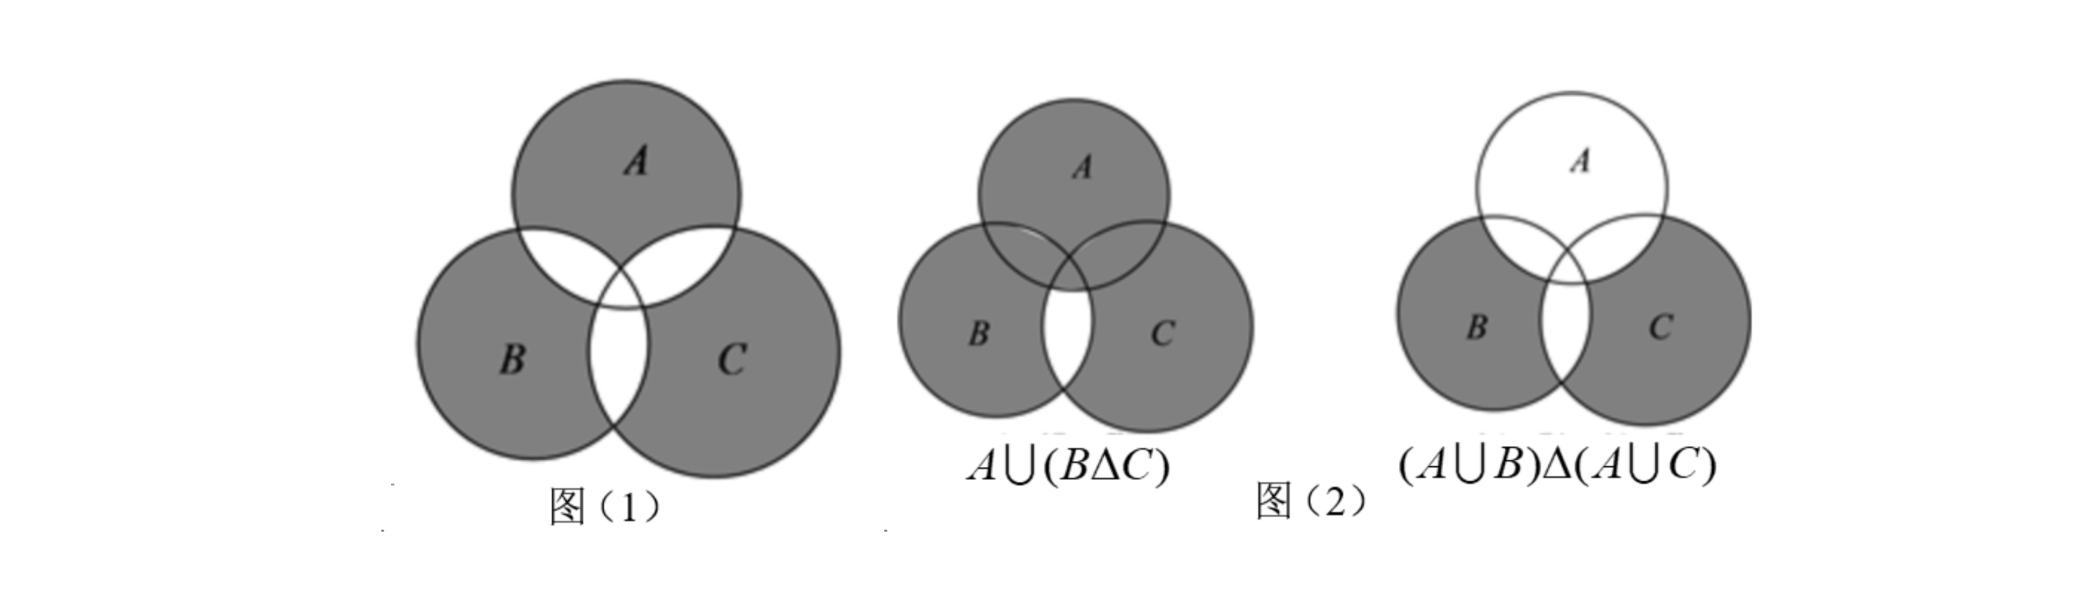
\includegraphics[width=0.92\textwidth]{figures/gao73_q16_symdiff.png}
\end{center}
\step{故选 $B$.}
\solend
\fi

\end{enumerate}

\bigsec{三、解答题}

\begin{enumerate}
\setcounter{enumi}{16}

\item （1）解不等式 $\dfrac{2-x}{x+3}>1$；

（2）已知 $a$ 是实数，试解关于 $x$ 的不等式：$x^2+(a-1)x-a\geqslant0$.

\ifanswer
\solbegin
\stepm{(1)}{$\dfrac{2-x}{x+3}-1=\dfrac{-2x-1}{x+3}>0$，则 $(2x+1)(x+3)<0$，得 $-3<x<-\dfrac12$，}
\step{所以不等式解集为 $\left(-3,-\dfrac12\right)$；}
\stepm{(2)}{$x^2+(a-1)x-a=(x+a)(x-1)\geqslant0$，}
% 原卷 (2) 题干为 ≥0，但解析按 ≤0 给出“两根之间”的解集，照录（见文件头“原卷笔误/存疑”②）
\step{当 $-a<1$，即 $a>-1$ 时，解集为 $(-a,1)$；}
\step{当 $-a=1$，即 $a=-1$ 时，解集为 $\R$；}
\step{当 $-a>1$，即 $a<-1$ 时，解集为 $(1,-a)$；}
\step{综上，当 $a>-1$ 时，解集为 $(-a,1)$；}
\step{当 $a=-1$ 时，解集为 $\R$；}
\step{当 $a<-1$ 时，解集为 $(1,-a)$.}
\solend
\fi

\ansspace[5]

\item （1）设 $a$、$b$ 是两个正数. 已知 $a>b$，比较 $\dfrac{2a+b}{a+2b}$ 与 $\dfrac ab$ 的值的大小；

（2）若实数 $a$ 满足 $\sqrt{(2023-a)^2}+\sqrt{a-2024}=a$，求 $a-2023^2$ 的值.

\ifanswer
\solbegin
\stepm{(1)}{$\dfrac{2a+b}{a+2b}-\dfrac ab=\dfrac{b^2-a^2}{b(a+2b)}<0$，所以 $\dfrac{2a+b}{a+2b}<\dfrac ab$.}
\stepm{(2)}{因为 $a-2024\geqslant0$，所以 $a\geqslant2024$，}
\step{所以 $\sqrt{(2023-a)^2}+\sqrt{a-2024}=a-2023+\sqrt{a-2024}$，}
\step{即 $a-2023+\sqrt{a-2024}=a$，即 $\sqrt{a-2024}=2023$，}
\step{所以 $a-2024=2023^2$，所以 $a-2023^2=2024$.}
\solend
\fi

\ansspace[5]

\item 已知 $m\in\R$，集合 $A=\{x\mid-1\leqslant x\leqslant3\}$，$B=\{x\mid m-3<x\leqslant m+2\}$.

（1）若“$x\in A$”是“$x\in B$”的充分不必要条件，求 $m$ 的取值范围；

（2）若 $A\cap B\neq\varnothing$，求 $m$ 的取值范围.

\ifanswer
\solbegin
\stepm{(1)}{因为“$x\in A$”是“$x\in B$”的充分不必要条件，所以 $A$ 是 $B$ 的真子集，}
\step{需满足 $\begin{cases}m-3<-1\\ m+2\geqslant3\end{cases}$，解得 $\begin{cases}m<2\\ m\geqslant1\end{cases}$，所以 $m$ 的取值范围是 $[1,2)$.}
\stepm{(2)}{因为 $A\cap B\neq\varnothing$，所以 $\begin{cases}m+2\geqslant-1\\ m-3<3\end{cases}$，解得 $\begin{cases}m\geqslant-3\\ m<6\end{cases}$，}
\step{所以 $m$ 的取值范围是 $[-3,6)$.}
\solend
\fi

\ansspace[6]

\item 已知集合 $A=\{x\mid x<-2\text{ 或 }x\geqslant3\}$，$U=\R$.

（1）若 $B=\{x\mid mx-1>0\}$，当 $B\subseteq A$ 时，求实数 $m$ 的取值范围；

（2）若 $B=\{x\mid2m-6\leqslant x\leqslant m+4\}$，当 $B\cap\overline A=\varnothing$ 时，求实数 $m$ 的取值范围.

\ifanswer
\solbegin
\stepm{(1)}{当 $m=0$ 时，$B=\varnothing$，符合题意，}
\step{当 $m>0$ 时，$B=\left\{x\mid x>\dfrac1m\right\}$，则 $\dfrac1m\geqslant3$，解得 $0<m\leqslant\dfrac13$，}
\step{当 $m<0$ 时，$B=\left\{x\mid x<\dfrac1m\right\}$，则 $\dfrac1m\leqslant-2$，解得 $-\dfrac12\leqslant m<0$，}
\step{综上所述，实数 $m$ 的取值范围 $\left[-\dfrac12,\dfrac13\right]$；}
\stepm{(2)}{由题意得 $B=\{x\mid2m-6\leqslant x\leqslant m+4\}$，$\overline A=\{x\mid-2\leqslant x<3\}$，且 $B\cap\overline A=\varnothing$，}
\step{当 $B=\varnothing$ 时，$2m-6>m+4$，解得 $m>10$，}
\step{当 $B\neq\varnothing$ 时，$\begin{cases}2m-6\leqslant m+4\\ m+4<-2\end{cases}$ 或 $\begin{cases}2m-6\leqslant m+4\\ 2m-6\geqslant3\end{cases}$，解得 $m<-6$ 或 $\dfrac92\leqslant m\leqslant10$，}
\step{综上所述，实数 $m$ 的取值范围为 $(-\infty,-6)\cup\left[\dfrac92,+\infty\right)$.}
\solend
\fi

\ansspace[7]

\item 关于实数大小关系的基本事实是解决等式或不等式问题的逻辑基础. 两个正数的大小关系是完全确定的，但通过运算就会产生非常奇妙的变化，基本不等式就是其中之一. 通过运算（代数变形）可以解决很多关于基本不等式的问题.

例如此题：正实数 $x$、$y$，满足 $x+y=1$，求 $\dfrac1x+\dfrac4y$ 的最小值. 求解本问题的方法很多，其中一种求解方法是：$\dfrac1x+\dfrac4y=(x+y)\left(\dfrac1x+\dfrac4y\right)=5+\dfrac yx+\dfrac{4x}{y}\geqslant5+2\sqrt{\dfrac yx\cdot\dfrac{4x}{y}}=9$，当且仅当 $\dfrac yx=\dfrac{4x}{y}$ 即 $y=2x$ 且 $x+y=1$ 时，即 $x=\dfrac13$，$y=\dfrac23$ 时等号成立.

这种解题方法叫作“$1$”的代换，利用上述求解方法解决下列问题：

（1）正数 $a$、$b$ 满足 $a+b=1$，求 $\dfrac1a+\dfrac2b$ 的最小值；

（2）已知 $a$、$b$、$c$ 均为正实数，且 $\dfrac1a+\dfrac1b+\dfrac1c=1$，求证：$a+b+c\geqslant9$；

（3）已知 $a$、$b$、$x$、$y$ 均为正实数，且 $\dfrac{x^2}{a^2}-\dfrac{y^2}{b^2}=1$，求证：$a^2-b^2\leqslant(x-y)^2$.

\ifanswer
\solbegin
\stepm{(1)}{正数 $a$、$b$ 满足 $a+b=1$，}
\step{$\dfrac1a+\dfrac2b=(a+b)\left(\dfrac1a+\dfrac2b\right)=1+2+\dfrac ba+\dfrac{2a}{b}\geqslant3+2\sqrt{\dfrac ba\cdot\dfrac{2a}{b}}=3+2\sqrt2$，}
\step{当且仅当 $\dfrac ba=\dfrac{2a}{b}$ 即 $b=\sqrt2\,a$ 且 $a+b=1$ 时，}
\step{即 $a=\sqrt2-1$，$b=2-\sqrt2$ 时取等号.}
\stepm{(2)}{$a+b+c=\left(\dfrac1a+\dfrac1b+\dfrac1c\right)(a+b+c)=3+\dfrac ba+\dfrac ab+\dfrac ca+\dfrac ac+\dfrac cb+\dfrac bc$}
\step{$\geqslant3+2\sqrt{\dfrac ba\cdot\dfrac ab}+2\sqrt{\dfrac ca\cdot\dfrac ac}+2\sqrt{\dfrac cb\cdot\dfrac bc}=9$，当且仅当 $a=b=c=3$ 时取等号，}
\step{故 $a+b+c\geqslant9$.}
\stepm{(3)}{$a^2-b^2=(a^2-b^2)\left(\dfrac{x^2}{a^2}-\dfrac{y^2}{b^2}\right)=x^2+y^2-\dfrac{b^2x^2}{a^2}-\dfrac{a^2y^2}{b^2}$}
\step{$=x^2+y^2-\left(\dfrac{b^2x^2}{a^2}+\dfrac{a^2y^2}{b^2}\right)\leqslant x^2+y^2-2\cdot\dfrac{bx}{a}\cdot\dfrac{ay}{b}=x^2+y^2-2xy$}
\step{$=(x-y)^2$，当且仅当 $\dfrac{bx}{a}=\dfrac{ay}{b}$ 且 $\dfrac{x^2}{a^2}-\dfrac{y^2}{b^2}=1$ 时，}
\step{即 $x=\dfrac{a^2}{\sqrt{a^2-b^2}}$，$y=\dfrac{b^2}{\sqrt{a^2-b^2}}$，$a>b$ 时取等号，故 $a^2-b^2\leqslant(x-y)^2$.}
\solend
\fi

\ansspace*[7]

\end{enumerate}

\end{document}
"
% 紧凑版：xelatex "\def\iscompact{1}% 高一73_徐汇中学_10月月考.tex
%   —— 高一上数学“2026-2027 年徐汇中学高一上 10 月月考”（讲评版）
% 试卷版：xelatex 高一73_徐汇中学_10月月考.tex
% 答案版：xelatex "\def\isanswer{1}\input{高一73_徐汇中学_10月月考.tex}"
% 紧凑版：xelatex "\def\iscompact{1}\input{高一73_徐汇中学_10月月考.tex}"
%
% 原始材料：微信公众号“魔都数学加油站”文章，连载“27学年高一73”；
% 原文标题“27学年高一73——2026-2027年上海市徐汇中学高一上10月月考”；
% 原文链接：https://mp.weixin.qq.com/s/Pkk9tFr4qHS9BR_BPxvk6A。
% 页面标注发布时间 2026-10-21 20:41（上海）。
% 正文为 10 张 PNG 页（`原图/高一73_徐汇中学_10月月考/01..10.png`）：
% 第 1、4、6、9、10 页为 2560×3620，其余 5 页为 4762×6735，均按页序读取。
% 10 页全为试卷正文页（卷首标题在第 1 页页顶，卷末第 21 题 (3) 解析止于第 10 页），
% 无封面页、目录页、二维码或宣传页。粉色斜排“魔都数学加油站”为卷面水印，未录入。
%
% 卷首标题：照卷面印作“2026-2027 年徐汇中学高一上 10 月月考”（黑体加粗一行）。
% 原卷年份区间用半角连字符，本稿按全稿惯例排 en dash；原卷无副标题。
%
% 篇幅与题号：原卷自第 3 题起编号（第 1、2 题不在本卷内）。填空题 3—12（10 题）、
% 选择题 13—16（4 题）、解答题 17—21（5 题），共 19 题。本稿沿用原节与原题号，
% 只改排为全稿统一的大节样式。
%
% 讲评版：原卷第 3、4 题只印【答案】（“没有实数根”“真”），本稿只给 \ans{}；
% 其余 17 题均印【解析】，用 \solbegin…\solend。四道选择题的作答括号原卷即留空，
% 答案写在解析末句“故选 A／D／A／B”，照录在解析内，不另提 \ans{}。
%
% 副标题：原卷未印副标题。本稿按“知识模块”口径标作“集合与常用逻辑用语、不等式”：
% 19 题中集合与常用逻辑用语 9 题（第 3、4、7、11、12、13、16、19、20 题），
% 不等式 10 题（第 5、6、8、9、10、14、15、17、18、21 题），两类均确有分量，故并标。
% 口径同 高一63、高一68—72。
%
% 与原卷的排版差异：
%   ① 原卷每题下直接印【答案】/【解析】，本稿按全稿惯例将答案与解析置于答案版；
%   ② 原卷未印副标题，本稿按“知识模块”口径补出；
%   ③ 原卷填空横线约四个字宽，本稿按全稿惯例统一排 \blankline[4.4em]；
%   ④ 原卷数集记号排斜体 $R$（第 3、8、9、10、12、17、19、20 题等），本稿按全稿惯例
%      改用 $\R$（同 高一68—72）；空集记号原卷作 $\varnothing$，照录；
%   ⑤ 原卷句末标点多为西文句点，第 15 题题干“整数解只有 $-2$”后为全角逗号，
%      均逐处照录；第 16 题解析的集合运算用 $\Delta$ 表示对称差，照原卷符号排；
%   ⑥ 第 17—21 题的子问原卷印作“（1）…（2）…”，本稿按 高一69—72 成例用行内
%      “（1）（2）（3）”段，解析中的子问标号用 \stepm{(1)}{…}；
%   ⑦ 每道解答题原卷未留作答空白，本稿按全稿惯例加 \ansspace（末题用 \ansspace*）；
%   ⑧ 选择题的作答括号原卷排半角“(    )”，本稿按全稿惯例排 \mbox{（\quad）}；
%      选项行排照原卷——第 13 题一行四条、第 14—16 题一行四条；
%   ⑨ 第 15 题题干的不等式组、第 14、19、20 题解析中的不等式组，原卷均排作“{”
%      连接的多行式，本稿按全稿惯例排 cases；
%   ⑩ 第 16 题解析末尾有三幅韦恩图（图（1）与图（2）的两幅）：原卷印在【解析】中，
%      题干无“如图”二字。本稿按原卷截图裁取（`figures/gao73_q16_symdiff.png`，
%      由第 6 页原图裁出、去除粉色水印后转灰度，未放大），放在答案版解析④之后。
%
% 原卷笔误/存疑（均照录未改，正文对应处另有 % 注）：
%   ① 第 3 题题干“设 $a$、$b\in\R$，则方程 $x^2+ax+a-1=0$ 至少有一个实根”中
%      $b$ 未在方程或后文出现，疑为衍字；原卷如此，照录未改。
%   ② 第 17 题 (2) 题干为 $x^2+(a-1)x-a\geqslant0$，但解析按 $\leqslant0$ 给出解集：
%      $a>-1$ 时写 $(-a,1)$、$a<-1$ 时写 $(1,-a)$，恰是“两根之间”的区间。
%      按题干 $\geqslant0$ 应为 $(-\infty,-a]\cup[1,+\infty)$ 与 $(-\infty,1]\cup[-a,+\infty)$；
%      原卷如此，照录未改。
%
% 行数核对：逐题数 \step/\stepm 条数与原卷【解析】印刷行数，17 题逐一相符，
% 合计 104 条 / 104 行（Q5：1；Q6：2；Q7：4；Q8：4；Q9：3；Q10：4；Q11：8；
% Q12：7；Q13：7；Q14：5；Q15：7；Q16：15；Q17：9；Q18：5；Q19：4；Q20：8；Q21：11）。
% 另第 3、4 题只印【答案】，各提 \ans{}，不计入 \step 账。
%
% 插图：第 16 题解析末的 3 幅韦恩图，见上⑩；全卷题干无其他配图。
%
\documentclass[a4paper,11pt]{article}
\usepackage{common}

\begin{document}

\examtitlest[3]{2026--2027 年徐汇中学高一上 10 月月考}{集合与常用逻辑用语、不等式}

\bigsec{一、填空题}

\begin{enumerate}
\setcounter{enumi}{2}

% 原卷题干“设 a、b∈R”中的 b 未在方程中出现，照录（见文件头“原卷笔误/存疑”①）
\item 如果用反证法证明命题“设 $a$、$b\in\R$，则方程 $x^2+ax+a-1=0$ 至少有一个实根”，那么首先假设方程 $x^2+ax+a-1=0$\blankline[4.4em].

\ifanswer
\ans{没有实数根}
\fi

\item 命题“若 $\dfrac1x>1$，则 $x<1$”是\blankline[4.4em]命题（填“真”，“假”）.

\ifanswer
\ans{真}
\fi

\item 对数 $\log_a(5-a)$ 中实数 $a$ 的取值范围是\blankline[4.4em].

\ifanswer
\solbegin
\step{由对数定义得 $\begin{cases}a>0\\ a\neq1\\ 5-a>0\end{cases}$，解得 $0<a<1$ 或 $1<a<5$.}
\solend
\fi

\item 关于 $x$ 的不等式 $ax^2-(a+1)x+1\leqslant0\,(a<0)$ 的解集为\blankline[4.4em].

\ifanswer
\solbegin
\step{原不等式即 $(ax-1)(x-1)\leqslant0$，因为 $a<0$，所以 $\left(x-\dfrac1a\right)(x-1)\geqslant0$.}
\step{又 $\dfrac1a<0<1$，所以 $x\leqslant\dfrac1a$ 或 $x\geqslant1$，故解集为 $\left(-\infty,\dfrac1a\right]\cup[1,+\infty)$.}
\solend
\fi

\item 若集合 $A=\{x\mid x^2-2kx+7k=0\}$ 有且仅有三个真子集，则 $k$ 的取值范围是\blankline[4.4em].

\ifanswer
\solbegin
\step{因为集合 $A$ 有且仅有三个真子集，则 $2^n-1=3$，解得 $n=2$，}
\step{所以一元二次方程 $x^2-2kx+7k=0$ 有两个不同的实数解，}
\step{则 $\Delta=4k^2-28k>0$，解得 $k<0$ 或 $k>7$，}
\step{故 $k$ 的取值范围是 $(-\infty,0)\cup(7,+\infty)$.}
\solend
\fi

\item 已知关于 $x$ 的不等式 $kx^2-4kx+k-6<0$ 对任意 $x\in\R$ 恒成立，则 $k$ 的取值范围是\blankline[4.4em].

\ifanswer
\solbegin
\step{关于 $x$ 的不等式 $kx^2-4kx+k-6<0$ 对任意 $x\in\R$ 恒成立，}
\step{当 $k=0$ 时，$kx^2-4kx+k-6=-6<0$ 恒成立，}
\step{当 $k\neq0$ 时，则 $\begin{cases}\Delta=16k^2-4k(k-6)<0\\ k<0\end{cases}$，解得 $-2<k<0$，}
\step{综上，$k$ 的取值范围为 $(-2,0]$.}
\solend
\fi

\item 设 $x\in\R$，方程 $|x-1|+|2x-1|=|3x-2|$ 的解集为\blankline[4.4em].

\ifanswer
\solbegin
\step{因为 $|x-1|+|2x-1|\geqslant|(x-1)+(2x-1)|=|3x-2|$，}
\step{当且仅当 $(x-1)(2x-1)\geqslant0$，解得 $x\leqslant\dfrac12$ 或 $x\geqslant1$，}
\step{故方程 $|x-1|+|2x-1|=|3x-2|$ 的解集为 $\left(-\infty,\dfrac12\right]\cup[1,+\infty)$.}
\solend
\fi

\item 已知 $a\in\R$，若关于 $x$ 的方程 $x^2+ax+a^2-8=0$ 有两个实根 $x_1$、$x_2$，且 $\dfrac1{x_1}+\dfrac1{x_2}=-\dfrac12$，则 $a$ 的值为\blankline[4.4em].

\ifanswer
\solbegin
\step{由题意得 $\Delta=a^2-4(a^2-8)=32-3a^2\geqslant0$，解得 $a^2\leqslant\dfrac{32}3$，}
\step{由韦达定理得 $x_1+x_2=-a$，$x_1x_2=a^2-8$，}
\step{则 $\dfrac1{x_1}+\dfrac1{x_2}=\dfrac{x_1+x_2}{x_1x_2}=\dfrac{-a}{a^2-8}=-\dfrac12$，即 $a^2-2a-8=(a-4)(a+2)=0$，}
\step{解得 $a=4$ 或 $a=-2$. 又 $a^2\leqslant\dfrac{32}3$，则 $a=-2$.}
\solend
\fi

\item 甲、乙两人解关于 $x$ 的不等式 $x^2+bx+c<0$，甲写错了 $b$，正确计算后得到的解为 $\{x\mid1<x<2\}$；乙写错了 $c$，正确计算后得到的解为 $\{x\mid-4<x<1\}$. 那么不等式 $\dfrac{bx+c}{x-2}<0$ 的解为\blankline[4.4em].

\ifanswer
\solbegin
\step{由 $x^2+bx+c<0$ 的解为 $\{x\mid1<x<2\}$，}
\step{则 $1$ 和 $2$ 是方程 $x^2+bx+c=0$ 的两个根，}
\step{甲写错了 $b$，但 $c$ 是正确的，所以 $c=1\times2=2$；}
\step{由 $x^2+bx+c<0$ 的解为 $\{x\mid-4<x<1\}$，}
\step{则 $-4$ 和 $1$ 是方程 $x^2+bx+c=0$ 的两个根，}
\step{乙写错了 $c$，但 $b$ 是正确的，所以 $-b=-4+1=-3$，即 $b=3$.}
\step{由 $\dfrac{bx+c}{x-2}<0$，得 $\dfrac{3x+2}{x-2}<0$，即 $(3x+2)(x-2)<0$，解得 $-\dfrac23<x<2$，}
\step{所以不等式 $\dfrac{bx+c}{x-2}<0$ 的解为 $\left\{x\mid-\dfrac23<x<2\right\}$.}
\solend
\fi

\item 设 $a,b,c\in\R$，$S=\{x\mid(x+a)(x^2+bx+c)=0,x\in\R\}$，$T=\{x\mid(ax+1)(cx^2+bx+1)=0,x\in\R\}$. 若 $|S|$、$|T|$ 分别为集合 $S$、$T$ 的元素个数，则 $|S|+|T|$ 的所有可能取值组成的集合为\blankline[4.4em].

\ifanswer
\solbegin
\step{$x\neq0$ 时，$(ax+1)(cx^2+bx+1)=x^3\left(\dfrac1x+a\right)\left(\dfrac1{x^2}+\dfrac bx+c\right)$，}
\step{故 $S$、$T$ 的非零元按倒数一一对应，设其个数均为 $k$；}
\step{$0\notin T$，且 $0\in S\Leftrightarrow ac=0$. 当 $ac=0$ 时 $k\in\{0,1,2\}$，}
\step{当 $ac\neq0$ 时 $x=-a\neq0$ 是 $S$ 的非零元，$k\in\{1,2,3\}$.}
\step{因此 $|S|+|T|$ 分别可取 $2k+1\in\{1,3,5\}$ 与 $2k\in\{2,4,6\}$.}
\step{依次取 $(a,b,c)=(0,0,0),(1,0,1),(0,-2,1),(1,-2,1),(0,0,-1),(1,-5,6)$，可分别实现 $1,2,3,4,5,6$，}
\step{则 $|S|+|T|$ 的所有可能取值组成的集合为 $\{1,2,3,4,5,6\}$.}
\solend
\fi

\end{enumerate}

\bigsec{二、选择题}

\begin{enumerate}
\setcounter{enumi}{12}

\item 如果 $a>b$，$c\neq0$，那么下列不等式成立的是\mbox{（\quad）}

\keepwithprev
A. $a-c>b-c$\qquad B. $c-a>c-b$\qquad C. $ac>bc$\qquad D. $\dfrac ac>\dfrac bc$

\ifanswer
\solbegin
\step{对于 $A$：$a-c-(b-c)=a-b>0$，即 $a-c>b-c$，故 $A$ 正确；}
\step{对于 $B$：$c-a-(c-b)=b-a<0$，即 $c-a<c-b$，故 $B$ 错误；}
\step{对于 $C$：$ac-bc=c(a-b)$，已知 $a-b>0$，}
\step{当 $c<0$ 时，$c(a-b)<0$，此时 $ac<bc$，故 $C$ 错误；}
\step{对于 $D$：$\dfrac ac-\dfrac bc=\dfrac1c(a-b)$，已知 $a-b>0$，}
\step{当 $c<0$ 时，$\dfrac1c(a-b)<0$，此时 $\dfrac ac<\dfrac bc$，故 $D$ 错误.}
\step{故选 $A$.}
\solend
\fi

\item 若不等式 $|x+1|\leqslant a$ 成立的一个充分不必要条件是 $-3\leqslant x\leqslant4$，则整数 $a$ 的最小值为\mbox{（\quad）}

\keepwithprev
A. $2$\qquad B. $3$\qquad C. $4$\qquad D. $5$

\ifanswer
\solbegin
\step{若 $a<0$，则 $|x+1|\leqslant a$ 无解；}
\step{若 $a\geqslant0$，由 $|x+1|\leqslant a$，得 $-1-a\leqslant x\leqslant-1+a$，}
\step{因为 $|x+1|\leqslant a$ 成立的一个充分不必要条件是 $-3\leqslant x\leqslant4$，}
\step{所以 $\begin{cases}-1-a\leqslant-3\\ -1+a\geqslant4\end{cases}$，等号不同时成立，解得 $a\geqslant5$，}
\step{故整数 $a$ 的最小值为 $5$. 故选 $D$.}
\solend
\fi

\item 若关于 $x$ 的不等式组 $\begin{cases}x^2-x-2>0\\ 2x^2+(5+2k)x+5k<0\end{cases}$ 的整数解只有 $-2$，则实数 $k$ 的取值范围为\mbox{（\quad）}

\keepwithprev
A. $[-3,2)$\qquad B. $[1,2]$\qquad C. $(1,2]$\qquad D. $(1,2)$

\ifanswer
\solbegin
\step{由 $x^2-x-2>0$，得 $x>2$ 或 $x<-1$，}
\step{由 $2x^2+(2k+5)x+5k<0$，得 $(2x+5)(x+k)<0$.}
\step{①若 $-k<-\dfrac52$，即 $k>\dfrac52$ 时，解得 $-k<x<-\dfrac52$，}
\step{此时原不等式的解集为 $\left(-k,-\dfrac52\right)$，不符合题意；}
\step{②若 $k=\dfrac52$ 时，解得 $x\in\varnothing$，显然不符合题意；}
\step{③若 $k<\dfrac52$ 时，解得 $-\dfrac52<x<-k$，则 $-2<-k\leqslant3$，即 $-3\leqslant k<2$.}
\step{综上，实数 $k$ 的取值范围 $[-3,2)$. 故选 $A$.}
\solend
\fi

\item 定义集合运算 $A-B=\{x\mid x\in A\text{ 且 }x\notin B\}$ 称为集合 $A$ 与集合 $B$ 的差集；定义集合运算 $A\Delta B=(A-B)\cup(B-A)$ 称为集合 $A$ 与集合 $B$ 的对称差，有以下 $4$ 个等式：

① $A\Delta B=B\Delta A$；

② $(A\Delta B)\Delta C=A\Delta(B\Delta C)$；

③ $A\cap(B\Delta C)=(A\cap B)\Delta(A\cap C)$；

④ $A\cup(B\Delta C)=(A\cup B)\Delta(A\cup C)$.

则 $4$ 个等式中恒成立的是\mbox{（\quad）}

\keepwithprev
A. ①②\qquad B. ①②③\qquad C. ①②④\qquad D. ①②③④

\ifanswer
\solbegin
\step{对于①，由 $B\Delta A=(B-A)\cup(A-B)=(A-B)\cup(B-A)=A\Delta B$，}
\step{所以①正确；}
\step{对于②，}
\step{由 $A-B=\{x\mid x\in A\text{ 且 }x\notin B\}=\{x\mid x\in A,x\notin(A\cap B)\}=A-(A\cap B)$，}
\step{同理可得 $B-A=B-(A\cap B)$，}
\step{则 $A\Delta B=(A-B)\cup(B-A)=(A\cup B)-(A\cap B)$，}
\step{所以 $(A\Delta B)\Delta C=(A\Delta B)\cup C-(A\Delta B)\cap C$，}
\step{所以表示的集合为图（1）中阴影部分所表示的集合，如图所示，}
\step{同理 $A\Delta(B\Delta C)=A\cup(B\Delta C)-A\cap(B\Delta C)$，}
\step{也表示图（1）中阴影部分所表示的集合，}
\step{所以 $(A\Delta B)\Delta C=A\Delta(B\Delta C)$，所以②正确；}
\step{对于③，由 $A\cap(B\Delta C)=A\cap(B\cup C-B\cap C)=A\cap(B\cup C)-A\cap(B\cap C)$}
\step{$=(A\cap B)\cup(A\cap C)-(A\cap B)\cap(A\cap C)=(A\cap B)\Delta(A\cap C)$，所以③正确；}
\step{对于④，如图（2）所示，$A\cup(B\Delta C)\neq(A\cup B)\Delta(A\cup C)$，所以④错误.}
\begin{center}
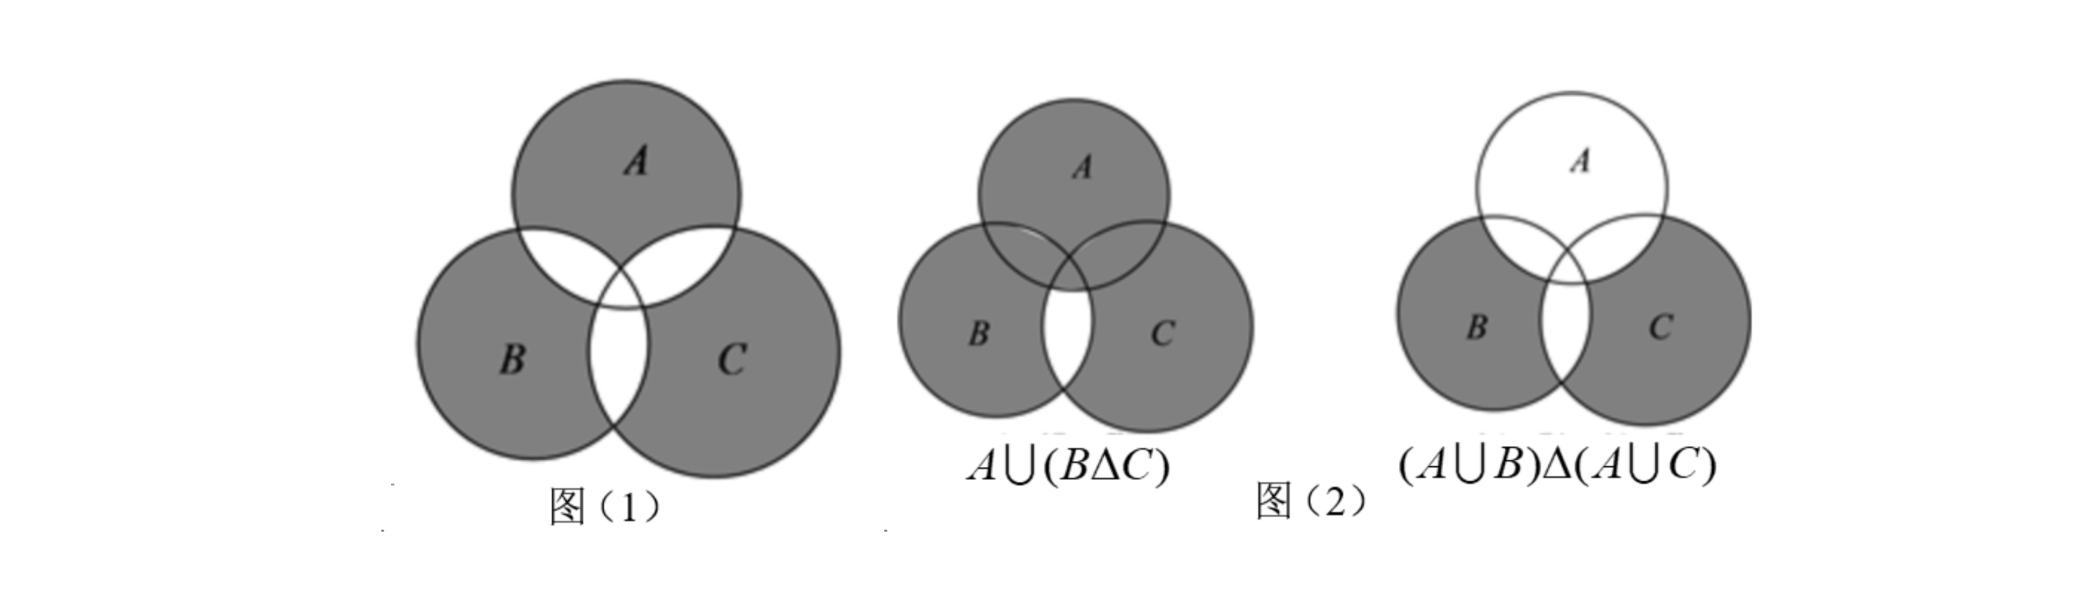
\includegraphics[width=0.92\textwidth]{figures/gao73_q16_symdiff.png}
\end{center}
\step{故选 $B$.}
\solend
\fi

\end{enumerate}

\bigsec{三、解答题}

\begin{enumerate}
\setcounter{enumi}{16}

\item （1）解不等式 $\dfrac{2-x}{x+3}>1$；

（2）已知 $a$ 是实数，试解关于 $x$ 的不等式：$x^2+(a-1)x-a\geqslant0$.

\ifanswer
\solbegin
\stepm{(1)}{$\dfrac{2-x}{x+3}-1=\dfrac{-2x-1}{x+3}>0$，则 $(2x+1)(x+3)<0$，得 $-3<x<-\dfrac12$，}
\step{所以不等式解集为 $\left(-3,-\dfrac12\right)$；}
\stepm{(2)}{$x^2+(a-1)x-a=(x+a)(x-1)\geqslant0$，}
% 原卷 (2) 题干为 ≥0，但解析按 ≤0 给出“两根之间”的解集，照录（见文件头“原卷笔误/存疑”②）
\step{当 $-a<1$，即 $a>-1$ 时，解集为 $(-a,1)$；}
\step{当 $-a=1$，即 $a=-1$ 时，解集为 $\R$；}
\step{当 $-a>1$，即 $a<-1$ 时，解集为 $(1,-a)$；}
\step{综上，当 $a>-1$ 时，解集为 $(-a,1)$；}
\step{当 $a=-1$ 时，解集为 $\R$；}
\step{当 $a<-1$ 时，解集为 $(1,-a)$.}
\solend
\fi

\ansspace[5]

\item （1）设 $a$、$b$ 是两个正数. 已知 $a>b$，比较 $\dfrac{2a+b}{a+2b}$ 与 $\dfrac ab$ 的值的大小；

（2）若实数 $a$ 满足 $\sqrt{(2023-a)^2}+\sqrt{a-2024}=a$，求 $a-2023^2$ 的值.

\ifanswer
\solbegin
\stepm{(1)}{$\dfrac{2a+b}{a+2b}-\dfrac ab=\dfrac{b^2-a^2}{b(a+2b)}<0$，所以 $\dfrac{2a+b}{a+2b}<\dfrac ab$.}
\stepm{(2)}{因为 $a-2024\geqslant0$，所以 $a\geqslant2024$，}
\step{所以 $\sqrt{(2023-a)^2}+\sqrt{a-2024}=a-2023+\sqrt{a-2024}$，}
\step{即 $a-2023+\sqrt{a-2024}=a$，即 $\sqrt{a-2024}=2023$，}
\step{所以 $a-2024=2023^2$，所以 $a-2023^2=2024$.}
\solend
\fi

\ansspace[5]

\item 已知 $m\in\R$，集合 $A=\{x\mid-1\leqslant x\leqslant3\}$，$B=\{x\mid m-3<x\leqslant m+2\}$.

（1）若“$x\in A$”是“$x\in B$”的充分不必要条件，求 $m$ 的取值范围；

（2）若 $A\cap B\neq\varnothing$，求 $m$ 的取值范围.

\ifanswer
\solbegin
\stepm{(1)}{因为“$x\in A$”是“$x\in B$”的充分不必要条件，所以 $A$ 是 $B$ 的真子集，}
\step{需满足 $\begin{cases}m-3<-1\\ m+2\geqslant3\end{cases}$，解得 $\begin{cases}m<2\\ m\geqslant1\end{cases}$，所以 $m$ 的取值范围是 $[1,2)$.}
\stepm{(2)}{因为 $A\cap B\neq\varnothing$，所以 $\begin{cases}m+2\geqslant-1\\ m-3<3\end{cases}$，解得 $\begin{cases}m\geqslant-3\\ m<6\end{cases}$，}
\step{所以 $m$ 的取值范围是 $[-3,6)$.}
\solend
\fi

\ansspace[6]

\item 已知集合 $A=\{x\mid x<-2\text{ 或 }x\geqslant3\}$，$U=\R$.

（1）若 $B=\{x\mid mx-1>0\}$，当 $B\subseteq A$ 时，求实数 $m$ 的取值范围；

（2）若 $B=\{x\mid2m-6\leqslant x\leqslant m+4\}$，当 $B\cap\overline A=\varnothing$ 时，求实数 $m$ 的取值范围.

\ifanswer
\solbegin
\stepm{(1)}{当 $m=0$ 时，$B=\varnothing$，符合题意，}
\step{当 $m>0$ 时，$B=\left\{x\mid x>\dfrac1m\right\}$，则 $\dfrac1m\geqslant3$，解得 $0<m\leqslant\dfrac13$，}
\step{当 $m<0$ 时，$B=\left\{x\mid x<\dfrac1m\right\}$，则 $\dfrac1m\leqslant-2$，解得 $-\dfrac12\leqslant m<0$，}
\step{综上所述，实数 $m$ 的取值范围 $\left[-\dfrac12,\dfrac13\right]$；}
\stepm{(2)}{由题意得 $B=\{x\mid2m-6\leqslant x\leqslant m+4\}$，$\overline A=\{x\mid-2\leqslant x<3\}$，且 $B\cap\overline A=\varnothing$，}
\step{当 $B=\varnothing$ 时，$2m-6>m+4$，解得 $m>10$，}
\step{当 $B\neq\varnothing$ 时，$\begin{cases}2m-6\leqslant m+4\\ m+4<-2\end{cases}$ 或 $\begin{cases}2m-6\leqslant m+4\\ 2m-6\geqslant3\end{cases}$，解得 $m<-6$ 或 $\dfrac92\leqslant m\leqslant10$，}
\step{综上所述，实数 $m$ 的取值范围为 $(-\infty,-6)\cup\left[\dfrac92,+\infty\right)$.}
\solend
\fi

\ansspace[7]

\item 关于实数大小关系的基本事实是解决等式或不等式问题的逻辑基础. 两个正数的大小关系是完全确定的，但通过运算就会产生非常奇妙的变化，基本不等式就是其中之一. 通过运算（代数变形）可以解决很多关于基本不等式的问题.

例如此题：正实数 $x$、$y$，满足 $x+y=1$，求 $\dfrac1x+\dfrac4y$ 的最小值. 求解本问题的方法很多，其中一种求解方法是：$\dfrac1x+\dfrac4y=(x+y)\left(\dfrac1x+\dfrac4y\right)=5+\dfrac yx+\dfrac{4x}{y}\geqslant5+2\sqrt{\dfrac yx\cdot\dfrac{4x}{y}}=9$，当且仅当 $\dfrac yx=\dfrac{4x}{y}$ 即 $y=2x$ 且 $x+y=1$ 时，即 $x=\dfrac13$，$y=\dfrac23$ 时等号成立.

这种解题方法叫作“$1$”的代换，利用上述求解方法解决下列问题：

（1）正数 $a$、$b$ 满足 $a+b=1$，求 $\dfrac1a+\dfrac2b$ 的最小值；

（2）已知 $a$、$b$、$c$ 均为正实数，且 $\dfrac1a+\dfrac1b+\dfrac1c=1$，求证：$a+b+c\geqslant9$；

（3）已知 $a$、$b$、$x$、$y$ 均为正实数，且 $\dfrac{x^2}{a^2}-\dfrac{y^2}{b^2}=1$，求证：$a^2-b^2\leqslant(x-y)^2$.

\ifanswer
\solbegin
\stepm{(1)}{正数 $a$、$b$ 满足 $a+b=1$，}
\step{$\dfrac1a+\dfrac2b=(a+b)\left(\dfrac1a+\dfrac2b\right)=1+2+\dfrac ba+\dfrac{2a}{b}\geqslant3+2\sqrt{\dfrac ba\cdot\dfrac{2a}{b}}=3+2\sqrt2$，}
\step{当且仅当 $\dfrac ba=\dfrac{2a}{b}$ 即 $b=\sqrt2\,a$ 且 $a+b=1$ 时，}
\step{即 $a=\sqrt2-1$，$b=2-\sqrt2$ 时取等号.}
\stepm{(2)}{$a+b+c=\left(\dfrac1a+\dfrac1b+\dfrac1c\right)(a+b+c)=3+\dfrac ba+\dfrac ab+\dfrac ca+\dfrac ac+\dfrac cb+\dfrac bc$}
\step{$\geqslant3+2\sqrt{\dfrac ba\cdot\dfrac ab}+2\sqrt{\dfrac ca\cdot\dfrac ac}+2\sqrt{\dfrac cb\cdot\dfrac bc}=9$，当且仅当 $a=b=c=3$ 时取等号，}
\step{故 $a+b+c\geqslant9$.}
\stepm{(3)}{$a^2-b^2=(a^2-b^2)\left(\dfrac{x^2}{a^2}-\dfrac{y^2}{b^2}\right)=x^2+y^2-\dfrac{b^2x^2}{a^2}-\dfrac{a^2y^2}{b^2}$}
\step{$=x^2+y^2-\left(\dfrac{b^2x^2}{a^2}+\dfrac{a^2y^2}{b^2}\right)\leqslant x^2+y^2-2\cdot\dfrac{bx}{a}\cdot\dfrac{ay}{b}=x^2+y^2-2xy$}
\step{$=(x-y)^2$，当且仅当 $\dfrac{bx}{a}=\dfrac{ay}{b}$ 且 $\dfrac{x^2}{a^2}-\dfrac{y^2}{b^2}=1$ 时，}
\step{即 $x=\dfrac{a^2}{\sqrt{a^2-b^2}}$，$y=\dfrac{b^2}{\sqrt{a^2-b^2}}$，$a>b$ 时取等号，故 $a^2-b^2\leqslant(x-y)^2$.}
\solend
\fi

\ansspace*[7]

\end{enumerate}

\end{document}
"
%
% 原始材料：微信公众号“魔都数学加油站”文章，连载“27学年高一73”；
% 原文标题“27学年高一73——2026-2027年上海市徐汇中学高一上10月月考”；
% 原文链接：https://mp.weixin.qq.com/s/Pkk9tFr4qHS9BR_BPxvk6A。
% 页面标注发布时间 2026-10-21 20:41（上海）。
% 正文为 10 张 PNG 页（`原图/高一73_徐汇中学_10月月考/01..10.png`）：
% 第 1、4、6、9、10 页为 2560×3620，其余 5 页为 4762×6735，均按页序读取。
% 10 页全为试卷正文页（卷首标题在第 1 页页顶，卷末第 21 题 (3) 解析止于第 10 页），
% 无封面页、目录页、二维码或宣传页。粉色斜排“魔都数学加油站”为卷面水印，未录入。
%
% 卷首标题：照卷面印作“2026-2027 年徐汇中学高一上 10 月月考”（黑体加粗一行）。
% 原卷年份区间用半角连字符，本稿按全稿惯例排 en dash；原卷无副标题。
%
% 篇幅与题号：原卷自第 3 题起编号（第 1、2 题不在本卷内）。填空题 3—12（10 题）、
% 选择题 13—16（4 题）、解答题 17—21（5 题），共 19 题。本稿沿用原节与原题号，
% 只改排为全稿统一的大节样式。
%
% 讲评版：原卷第 3、4 题只印【答案】（“没有实数根”“真”），本稿只给 \ans{}；
% 其余 17 题均印【解析】，用 \solbegin…\solend。四道选择题的作答括号原卷即留空，
% 答案写在解析末句“故选 A／D／A／B”，照录在解析内，不另提 \ans{}。
%
% 副标题：原卷未印副标题。本稿按“知识模块”口径标作“集合与常用逻辑用语、不等式”：
% 19 题中集合与常用逻辑用语 9 题（第 3、4、7、11、12、13、16、19、20 题），
% 不等式 10 题（第 5、6、8、9、10、14、15、17、18、21 题），两类均确有分量，故并标。
% 口径同 高一63、高一68—72。
%
% 与原卷的排版差异：
%   ① 原卷每题下直接印【答案】/【解析】，本稿按全稿惯例将答案与解析置于答案版；
%   ② 原卷未印副标题，本稿按“知识模块”口径补出；
%   ③ 原卷填空横线约四个字宽，本稿按全稿惯例统一排 \blankline[4.4em]；
%   ④ 原卷数集记号排斜体 $R$（第 3、8、9、10、12、17、19、20 题等），本稿按全稿惯例
%      改用 $\R$（同 高一68—72）；空集记号原卷作 $\varnothing$，照录；
%   ⑤ 原卷句末标点多为西文句点，第 15 题题干“整数解只有 $-2$”后为全角逗号，
%      均逐处照录；第 16 题解析的集合运算用 $\Delta$ 表示对称差，照原卷符号排；
%   ⑥ 第 17—21 题的子问原卷印作“（1）…（2）…”，本稿按 高一69—72 成例用行内
%      “（1）（2）（3）”段，解析中的子问标号用 \stepm{(1)}{…}；
%   ⑦ 每道解答题原卷未留作答空白，本稿按全稿惯例加 \ansspace（末题用 \ansspace*）；
%   ⑧ 选择题的作答括号原卷排半角“(    )”，本稿按全稿惯例排 \mbox{（\quad）}；
%      选项行排照原卷——第 13 题一行四条、第 14—16 题一行四条；
%   ⑨ 第 15 题题干的不等式组、第 14、19、20 题解析中的不等式组，原卷均排作“{”
%      连接的多行式，本稿按全稿惯例排 cases；
%   ⑩ 第 16 题解析末尾有三幅韦恩图（图（1）与图（2）的两幅）：原卷印在【解析】中，
%      题干无“如图”二字。本稿按原卷截图裁取（`figures/gao73_q16_symdiff.png`，
%      由第 6 页原图裁出、去除粉色水印后转灰度，未放大），放在答案版解析④之后。
%
% 原卷笔误/存疑（均照录未改，正文对应处另有 % 注）：
%   ① 第 3 题题干“设 $a$、$b\in\R$，则方程 $x^2+ax+a-1=0$ 至少有一个实根”中
%      $b$ 未在方程或后文出现，疑为衍字；原卷如此，照录未改。
%   ② 第 17 题 (2) 题干为 $x^2+(a-1)x-a\geqslant0$，但解析按 $\leqslant0$ 给出解集：
%      $a>-1$ 时写 $(-a,1)$、$a<-1$ 时写 $(1,-a)$，恰是“两根之间”的区间。
%      按题干 $\geqslant0$ 应为 $(-\infty,-a]\cup[1,+\infty)$ 与 $(-\infty,1]\cup[-a,+\infty)$；
%      原卷如此，照录未改。
%
% 行数核对：逐题数 \step/\stepm 条数与原卷【解析】印刷行数，17 题逐一相符，
% 合计 104 条 / 104 行（Q5：1；Q6：2；Q7：4；Q8：4；Q9：3；Q10：4；Q11：8；
% Q12：7；Q13：7；Q14：5；Q15：7；Q16：15；Q17：9；Q18：5；Q19：4；Q20：8；Q21：11）。
% 另第 3、4 题只印【答案】，各提 \ans{}，不计入 \step 账。
%
% 插图：第 16 题解析末的 3 幅韦恩图，见上⑩；全卷题干无其他配图。
%
\documentclass[a4paper,11pt]{article}
\usepackage{common}

\begin{document}

\examtitlest[3]{2026--2027 年徐汇中学高一上 10 月月考}{集合与常用逻辑用语、不等式}

\bigsec{一、填空题}

\begin{enumerate}
\setcounter{enumi}{2}

% 原卷题干“设 a、b∈R”中的 b 未在方程中出现，照录（见文件头“原卷笔误/存疑”①）
\item 如果用反证法证明命题“设 $a$、$b\in\R$，则方程 $x^2+ax+a-1=0$ 至少有一个实根”，那么首先假设方程 $x^2+ax+a-1=0$\blankline[4.4em].

\ifanswer
\ans{没有实数根}
\fi

\item 命题“若 $\dfrac1x>1$，则 $x<1$”是\blankline[4.4em]命题（填“真”，“假”）.

\ifanswer
\ans{真}
\fi

\item 对数 $\log_a(5-a)$ 中实数 $a$ 的取值范围是\blankline[4.4em].

\ifanswer
\solbegin
\step{由对数定义得 $\begin{cases}a>0\\ a\neq1\\ 5-a>0\end{cases}$，解得 $0<a<1$ 或 $1<a<5$.}
\solend
\fi

\item 关于 $x$ 的不等式 $ax^2-(a+1)x+1\leqslant0\,(a<0)$ 的解集为\blankline[4.4em].

\ifanswer
\solbegin
\step{原不等式即 $(ax-1)(x-1)\leqslant0$，因为 $a<0$，所以 $\left(x-\dfrac1a\right)(x-1)\geqslant0$.}
\step{又 $\dfrac1a<0<1$，所以 $x\leqslant\dfrac1a$ 或 $x\geqslant1$，故解集为 $\left(-\infty,\dfrac1a\right]\cup[1,+\infty)$.}
\solend
\fi

\item 若集合 $A=\{x\mid x^2-2kx+7k=0\}$ 有且仅有三个真子集，则 $k$ 的取值范围是\blankline[4.4em].

\ifanswer
\solbegin
\step{因为集合 $A$ 有且仅有三个真子集，则 $2^n-1=3$，解得 $n=2$，}
\step{所以一元二次方程 $x^2-2kx+7k=0$ 有两个不同的实数解，}
\step{则 $\Delta=4k^2-28k>0$，解得 $k<0$ 或 $k>7$，}
\step{故 $k$ 的取值范围是 $(-\infty,0)\cup(7,+\infty)$.}
\solend
\fi

\item 已知关于 $x$ 的不等式 $kx^2-4kx+k-6<0$ 对任意 $x\in\R$ 恒成立，则 $k$ 的取值范围是\blankline[4.4em].

\ifanswer
\solbegin
\step{关于 $x$ 的不等式 $kx^2-4kx+k-6<0$ 对任意 $x\in\R$ 恒成立，}
\step{当 $k=0$ 时，$kx^2-4kx+k-6=-6<0$ 恒成立，}
\step{当 $k\neq0$ 时，则 $\begin{cases}\Delta=16k^2-4k(k-6)<0\\ k<0\end{cases}$，解得 $-2<k<0$，}
\step{综上，$k$ 的取值范围为 $(-2,0]$.}
\solend
\fi

\item 设 $x\in\R$，方程 $|x-1|+|2x-1|=|3x-2|$ 的解集为\blankline[4.4em].

\ifanswer
\solbegin
\step{因为 $|x-1|+|2x-1|\geqslant|(x-1)+(2x-1)|=|3x-2|$，}
\step{当且仅当 $(x-1)(2x-1)\geqslant0$，解得 $x\leqslant\dfrac12$ 或 $x\geqslant1$，}
\step{故方程 $|x-1|+|2x-1|=|3x-2|$ 的解集为 $\left(-\infty,\dfrac12\right]\cup[1,+\infty)$.}
\solend
\fi

\item 已知 $a\in\R$，若关于 $x$ 的方程 $x^2+ax+a^2-8=0$ 有两个实根 $x_1$、$x_2$，且 $\dfrac1{x_1}+\dfrac1{x_2}=-\dfrac12$，则 $a$ 的值为\blankline[4.4em].

\ifanswer
\solbegin
\step{由题意得 $\Delta=a^2-4(a^2-8)=32-3a^2\geqslant0$，解得 $a^2\leqslant\dfrac{32}3$，}
\step{由韦达定理得 $x_1+x_2=-a$，$x_1x_2=a^2-8$，}
\step{则 $\dfrac1{x_1}+\dfrac1{x_2}=\dfrac{x_1+x_2}{x_1x_2}=\dfrac{-a}{a^2-8}=-\dfrac12$，即 $a^2-2a-8=(a-4)(a+2)=0$，}
\step{解得 $a=4$ 或 $a=-2$. 又 $a^2\leqslant\dfrac{32}3$，则 $a=-2$.}
\solend
\fi

\item 甲、乙两人解关于 $x$ 的不等式 $x^2+bx+c<0$，甲写错了 $b$，正确计算后得到的解为 $\{x\mid1<x<2\}$；乙写错了 $c$，正确计算后得到的解为 $\{x\mid-4<x<1\}$. 那么不等式 $\dfrac{bx+c}{x-2}<0$ 的解为\blankline[4.4em].

\ifanswer
\solbegin
\step{由 $x^2+bx+c<0$ 的解为 $\{x\mid1<x<2\}$，}
\step{则 $1$ 和 $2$ 是方程 $x^2+bx+c=0$ 的两个根，}
\step{甲写错了 $b$，但 $c$ 是正确的，所以 $c=1\times2=2$；}
\step{由 $x^2+bx+c<0$ 的解为 $\{x\mid-4<x<1\}$，}
\step{则 $-4$ 和 $1$ 是方程 $x^2+bx+c=0$ 的两个根，}
\step{乙写错了 $c$，但 $b$ 是正确的，所以 $-b=-4+1=-3$，即 $b=3$.}
\step{由 $\dfrac{bx+c}{x-2}<0$，得 $\dfrac{3x+2}{x-2}<0$，即 $(3x+2)(x-2)<0$，解得 $-\dfrac23<x<2$，}
\step{所以不等式 $\dfrac{bx+c}{x-2}<0$ 的解为 $\left\{x\mid-\dfrac23<x<2\right\}$.}
\solend
\fi

\item 设 $a,b,c\in\R$，$S=\{x\mid(x+a)(x^2+bx+c)=0,x\in\R\}$，$T=\{x\mid(ax+1)(cx^2+bx+1)=0,x\in\R\}$. 若 $|S|$、$|T|$ 分别为集合 $S$、$T$ 的元素个数，则 $|S|+|T|$ 的所有可能取值组成的集合为\blankline[4.4em].

\ifanswer
\solbegin
\step{$x\neq0$ 时，$(ax+1)(cx^2+bx+1)=x^3\left(\dfrac1x+a\right)\left(\dfrac1{x^2}+\dfrac bx+c\right)$，}
\step{故 $S$、$T$ 的非零元按倒数一一对应，设其个数均为 $k$；}
\step{$0\notin T$，且 $0\in S\Leftrightarrow ac=0$. 当 $ac=0$ 时 $k\in\{0,1,2\}$，}
\step{当 $ac\neq0$ 时 $x=-a\neq0$ 是 $S$ 的非零元，$k\in\{1,2,3\}$.}
\step{因此 $|S|+|T|$ 分别可取 $2k+1\in\{1,3,5\}$ 与 $2k\in\{2,4,6\}$.}
\step{依次取 $(a,b,c)=(0,0,0),(1,0,1),(0,-2,1),(1,-2,1),(0,0,-1),(1,-5,6)$，可分别实现 $1,2,3,4,5,6$，}
\step{则 $|S|+|T|$ 的所有可能取值组成的集合为 $\{1,2,3,4,5,6\}$.}
\solend
\fi

\end{enumerate}

\bigsec{二、选择题}

\begin{enumerate}
\setcounter{enumi}{12}

\item 如果 $a>b$，$c\neq0$，那么下列不等式成立的是\mbox{（\quad）}

\keepwithprev
A. $a-c>b-c$\qquad B. $c-a>c-b$\qquad C. $ac>bc$\qquad D. $\dfrac ac>\dfrac bc$

\ifanswer
\solbegin
\step{对于 $A$：$a-c-(b-c)=a-b>0$，即 $a-c>b-c$，故 $A$ 正确；}
\step{对于 $B$：$c-a-(c-b)=b-a<0$，即 $c-a<c-b$，故 $B$ 错误；}
\step{对于 $C$：$ac-bc=c(a-b)$，已知 $a-b>0$，}
\step{当 $c<0$ 时，$c(a-b)<0$，此时 $ac<bc$，故 $C$ 错误；}
\step{对于 $D$：$\dfrac ac-\dfrac bc=\dfrac1c(a-b)$，已知 $a-b>0$，}
\step{当 $c<0$ 时，$\dfrac1c(a-b)<0$，此时 $\dfrac ac<\dfrac bc$，故 $D$ 错误.}
\step{故选 $A$.}
\solend
\fi

\item 若不等式 $|x+1|\leqslant a$ 成立的一个充分不必要条件是 $-3\leqslant x\leqslant4$，则整数 $a$ 的最小值为\mbox{（\quad）}

\keepwithprev
A. $2$\qquad B. $3$\qquad C. $4$\qquad D. $5$

\ifanswer
\solbegin
\step{若 $a<0$，则 $|x+1|\leqslant a$ 无解；}
\step{若 $a\geqslant0$，由 $|x+1|\leqslant a$，得 $-1-a\leqslant x\leqslant-1+a$，}
\step{因为 $|x+1|\leqslant a$ 成立的一个充分不必要条件是 $-3\leqslant x\leqslant4$，}
\step{所以 $\begin{cases}-1-a\leqslant-3\\ -1+a\geqslant4\end{cases}$，等号不同时成立，解得 $a\geqslant5$，}
\step{故整数 $a$ 的最小值为 $5$. 故选 $D$.}
\solend
\fi

\item 若关于 $x$ 的不等式组 $\begin{cases}x^2-x-2>0\\ 2x^2+(5+2k)x+5k<0\end{cases}$ 的整数解只有 $-2$，则实数 $k$ 的取值范围为\mbox{（\quad）}

\keepwithprev
A. $[-3,2)$\qquad B. $[1,2]$\qquad C. $(1,2]$\qquad D. $(1,2)$

\ifanswer
\solbegin
\step{由 $x^2-x-2>0$，得 $x>2$ 或 $x<-1$，}
\step{由 $2x^2+(2k+5)x+5k<0$，得 $(2x+5)(x+k)<0$.}
\step{①若 $-k<-\dfrac52$，即 $k>\dfrac52$ 时，解得 $-k<x<-\dfrac52$，}
\step{此时原不等式的解集为 $\left(-k,-\dfrac52\right)$，不符合题意；}
\step{②若 $k=\dfrac52$ 时，解得 $x\in\varnothing$，显然不符合题意；}
\step{③若 $k<\dfrac52$ 时，解得 $-\dfrac52<x<-k$，则 $-2<-k\leqslant3$，即 $-3\leqslant k<2$.}
\step{综上，实数 $k$ 的取值范围 $[-3,2)$. 故选 $A$.}
\solend
\fi

\item 定义集合运算 $A-B=\{x\mid x\in A\text{ 且 }x\notin B\}$ 称为集合 $A$ 与集合 $B$ 的差集；定义集合运算 $A\Delta B=(A-B)\cup(B-A)$ 称为集合 $A$ 与集合 $B$ 的对称差，有以下 $4$ 个等式：

① $A\Delta B=B\Delta A$；

② $(A\Delta B)\Delta C=A\Delta(B\Delta C)$；

③ $A\cap(B\Delta C)=(A\cap B)\Delta(A\cap C)$；

④ $A\cup(B\Delta C)=(A\cup B)\Delta(A\cup C)$.

则 $4$ 个等式中恒成立的是\mbox{（\quad）}

\keepwithprev
A. ①②\qquad B. ①②③\qquad C. ①②④\qquad D. ①②③④

\ifanswer
\solbegin
\step{对于①，由 $B\Delta A=(B-A)\cup(A-B)=(A-B)\cup(B-A)=A\Delta B$，}
\step{所以①正确；}
\step{对于②，}
\step{由 $A-B=\{x\mid x\in A\text{ 且 }x\notin B\}=\{x\mid x\in A,x\notin(A\cap B)\}=A-(A\cap B)$，}
\step{同理可得 $B-A=B-(A\cap B)$，}
\step{则 $A\Delta B=(A-B)\cup(B-A)=(A\cup B)-(A\cap B)$，}
\step{所以 $(A\Delta B)\Delta C=(A\Delta B)\cup C-(A\Delta B)\cap C$，}
\step{所以表示的集合为图（1）中阴影部分所表示的集合，如图所示，}
\step{同理 $A\Delta(B\Delta C)=A\cup(B\Delta C)-A\cap(B\Delta C)$，}
\step{也表示图（1）中阴影部分所表示的集合，}
\step{所以 $(A\Delta B)\Delta C=A\Delta(B\Delta C)$，所以②正确；}
\step{对于③，由 $A\cap(B\Delta C)=A\cap(B\cup C-B\cap C)=A\cap(B\cup C)-A\cap(B\cap C)$}
\step{$=(A\cap B)\cup(A\cap C)-(A\cap B)\cap(A\cap C)=(A\cap B)\Delta(A\cap C)$，所以③正确；}
\step{对于④，如图（2）所示，$A\cup(B\Delta C)\neq(A\cup B)\Delta(A\cup C)$，所以④错误.}
\begin{center}
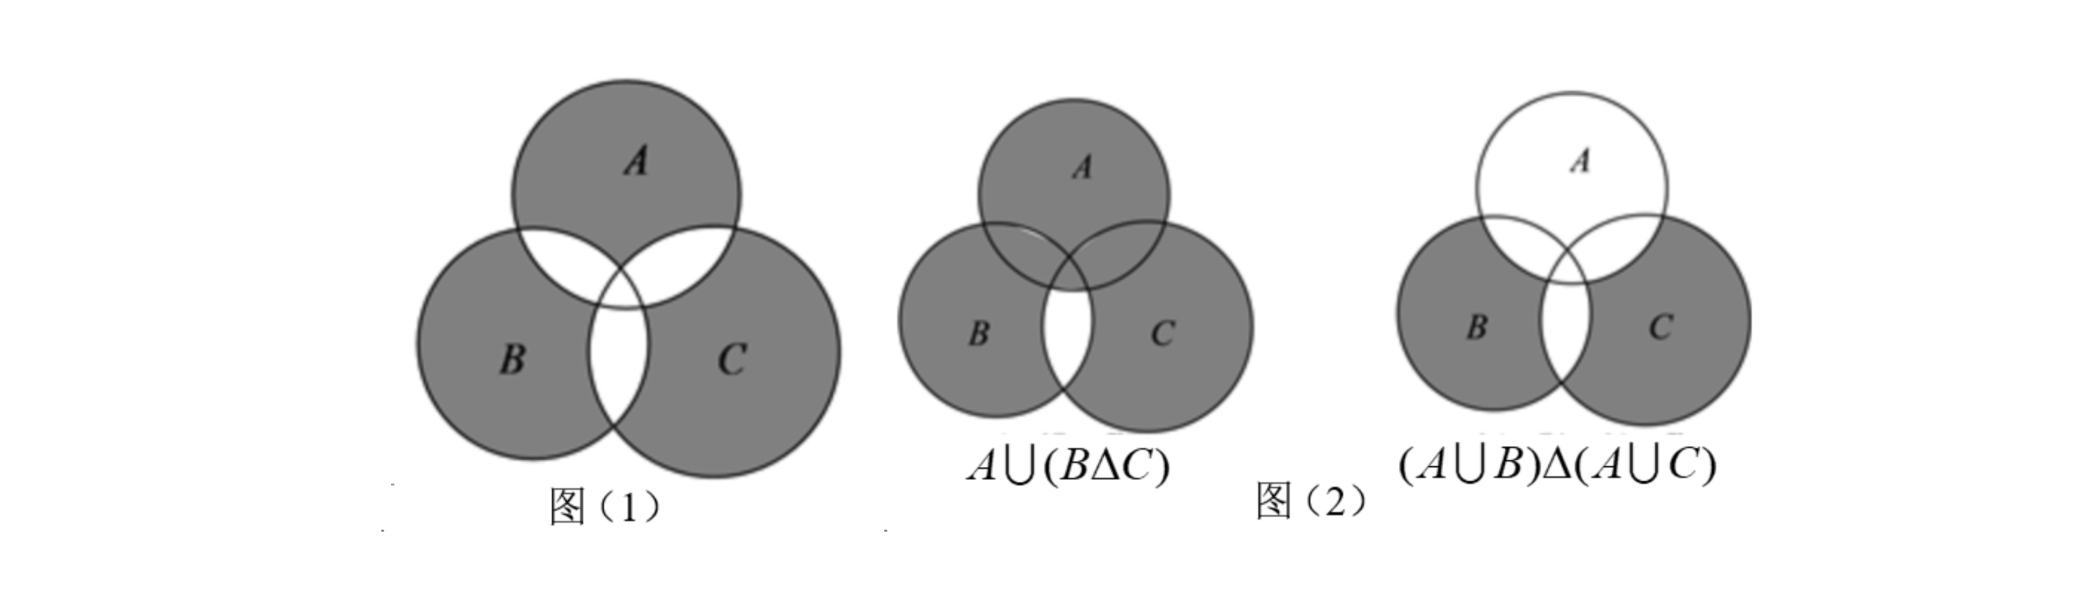
\includegraphics[width=0.92\textwidth]{figures/gao73_q16_symdiff.png}
\end{center}
\step{故选 $B$.}
\solend
\fi

\end{enumerate}

\bigsec{三、解答题}

\begin{enumerate}
\setcounter{enumi}{16}

\item （1）解不等式 $\dfrac{2-x}{x+3}>1$；

（2）已知 $a$ 是实数，试解关于 $x$ 的不等式：$x^2+(a-1)x-a\geqslant0$.

\ifanswer
\solbegin
\stepm{(1)}{$\dfrac{2-x}{x+3}-1=\dfrac{-2x-1}{x+3}>0$，则 $(2x+1)(x+3)<0$，得 $-3<x<-\dfrac12$，}
\step{所以不等式解集为 $\left(-3,-\dfrac12\right)$；}
\stepm{(2)}{$x^2+(a-1)x-a=(x+a)(x-1)\geqslant0$，}
% 原卷 (2) 题干为 ≥0，但解析按 ≤0 给出“两根之间”的解集，照录（见文件头“原卷笔误/存疑”②）
\step{当 $-a<1$，即 $a>-1$ 时，解集为 $(-a,1)$；}
\step{当 $-a=1$，即 $a=-1$ 时，解集为 $\R$；}
\step{当 $-a>1$，即 $a<-1$ 时，解集为 $(1,-a)$；}
\step{综上，当 $a>-1$ 时，解集为 $(-a,1)$；}
\step{当 $a=-1$ 时，解集为 $\R$；}
\step{当 $a<-1$ 时，解集为 $(1,-a)$.}
\solend
\fi

\ansspace[5]

\item （1）设 $a$、$b$ 是两个正数. 已知 $a>b$，比较 $\dfrac{2a+b}{a+2b}$ 与 $\dfrac ab$ 的值的大小；

（2）若实数 $a$ 满足 $\sqrt{(2023-a)^2}+\sqrt{a-2024}=a$，求 $a-2023^2$ 的值.

\ifanswer
\solbegin
\stepm{(1)}{$\dfrac{2a+b}{a+2b}-\dfrac ab=\dfrac{b^2-a^2}{b(a+2b)}<0$，所以 $\dfrac{2a+b}{a+2b}<\dfrac ab$.}
\stepm{(2)}{因为 $a-2024\geqslant0$，所以 $a\geqslant2024$，}
\step{所以 $\sqrt{(2023-a)^2}+\sqrt{a-2024}=a-2023+\sqrt{a-2024}$，}
\step{即 $a-2023+\sqrt{a-2024}=a$，即 $\sqrt{a-2024}=2023$，}
\step{所以 $a-2024=2023^2$，所以 $a-2023^2=2024$.}
\solend
\fi

\ansspace[5]

\item 已知 $m\in\R$，集合 $A=\{x\mid-1\leqslant x\leqslant3\}$，$B=\{x\mid m-3<x\leqslant m+2\}$.

（1）若“$x\in A$”是“$x\in B$”的充分不必要条件，求 $m$ 的取值范围；

（2）若 $A\cap B\neq\varnothing$，求 $m$ 的取值范围.

\ifanswer
\solbegin
\stepm{(1)}{因为“$x\in A$”是“$x\in B$”的充分不必要条件，所以 $A$ 是 $B$ 的真子集，}
\step{需满足 $\begin{cases}m-3<-1\\ m+2\geqslant3\end{cases}$，解得 $\begin{cases}m<2\\ m\geqslant1\end{cases}$，所以 $m$ 的取值范围是 $[1,2)$.}
\stepm{(2)}{因为 $A\cap B\neq\varnothing$，所以 $\begin{cases}m+2\geqslant-1\\ m-3<3\end{cases}$，解得 $\begin{cases}m\geqslant-3\\ m<6\end{cases}$，}
\step{所以 $m$ 的取值范围是 $[-3,6)$.}
\solend
\fi

\ansspace[6]

\item 已知集合 $A=\{x\mid x<-2\text{ 或 }x\geqslant3\}$，$U=\R$.

（1）若 $B=\{x\mid mx-1>0\}$，当 $B\subseteq A$ 时，求实数 $m$ 的取值范围；

（2）若 $B=\{x\mid2m-6\leqslant x\leqslant m+4\}$，当 $B\cap\overline A=\varnothing$ 时，求实数 $m$ 的取值范围.

\ifanswer
\solbegin
\stepm{(1)}{当 $m=0$ 时，$B=\varnothing$，符合题意，}
\step{当 $m>0$ 时，$B=\left\{x\mid x>\dfrac1m\right\}$，则 $\dfrac1m\geqslant3$，解得 $0<m\leqslant\dfrac13$，}
\step{当 $m<0$ 时，$B=\left\{x\mid x<\dfrac1m\right\}$，则 $\dfrac1m\leqslant-2$，解得 $-\dfrac12\leqslant m<0$，}
\step{综上所述，实数 $m$ 的取值范围 $\left[-\dfrac12,\dfrac13\right]$；}
\stepm{(2)}{由题意得 $B=\{x\mid2m-6\leqslant x\leqslant m+4\}$，$\overline A=\{x\mid-2\leqslant x<3\}$，且 $B\cap\overline A=\varnothing$，}
\step{当 $B=\varnothing$ 时，$2m-6>m+4$，解得 $m>10$，}
\step{当 $B\neq\varnothing$ 时，$\begin{cases}2m-6\leqslant m+4\\ m+4<-2\end{cases}$ 或 $\begin{cases}2m-6\leqslant m+4\\ 2m-6\geqslant3\end{cases}$，解得 $m<-6$ 或 $\dfrac92\leqslant m\leqslant10$，}
\step{综上所述，实数 $m$ 的取值范围为 $(-\infty,-6)\cup\left[\dfrac92,+\infty\right)$.}
\solend
\fi

\ansspace[7]

\item 关于实数大小关系的基本事实是解决等式或不等式问题的逻辑基础. 两个正数的大小关系是完全确定的，但通过运算就会产生非常奇妙的变化，基本不等式就是其中之一. 通过运算（代数变形）可以解决很多关于基本不等式的问题.

例如此题：正实数 $x$、$y$，满足 $x+y=1$，求 $\dfrac1x+\dfrac4y$ 的最小值. 求解本问题的方法很多，其中一种求解方法是：$\dfrac1x+\dfrac4y=(x+y)\left(\dfrac1x+\dfrac4y\right)=5+\dfrac yx+\dfrac{4x}{y}\geqslant5+2\sqrt{\dfrac yx\cdot\dfrac{4x}{y}}=9$，当且仅当 $\dfrac yx=\dfrac{4x}{y}$ 即 $y=2x$ 且 $x+y=1$ 时，即 $x=\dfrac13$，$y=\dfrac23$ 时等号成立.

这种解题方法叫作“$1$”的代换，利用上述求解方法解决下列问题：

（1）正数 $a$、$b$ 满足 $a+b=1$，求 $\dfrac1a+\dfrac2b$ 的最小值；

（2）已知 $a$、$b$、$c$ 均为正实数，且 $\dfrac1a+\dfrac1b+\dfrac1c=1$，求证：$a+b+c\geqslant9$；

（3）已知 $a$、$b$、$x$、$y$ 均为正实数，且 $\dfrac{x^2}{a^2}-\dfrac{y^2}{b^2}=1$，求证：$a^2-b^2\leqslant(x-y)^2$.

\ifanswer
\solbegin
\stepm{(1)}{正数 $a$、$b$ 满足 $a+b=1$，}
\step{$\dfrac1a+\dfrac2b=(a+b)\left(\dfrac1a+\dfrac2b\right)=1+2+\dfrac ba+\dfrac{2a}{b}\geqslant3+2\sqrt{\dfrac ba\cdot\dfrac{2a}{b}}=3+2\sqrt2$，}
\step{当且仅当 $\dfrac ba=\dfrac{2a}{b}$ 即 $b=\sqrt2\,a$ 且 $a+b=1$ 时，}
\step{即 $a=\sqrt2-1$，$b=2-\sqrt2$ 时取等号.}
\stepm{(2)}{$a+b+c=\left(\dfrac1a+\dfrac1b+\dfrac1c\right)(a+b+c)=3+\dfrac ba+\dfrac ab+\dfrac ca+\dfrac ac+\dfrac cb+\dfrac bc$}
\step{$\geqslant3+2\sqrt{\dfrac ba\cdot\dfrac ab}+2\sqrt{\dfrac ca\cdot\dfrac ac}+2\sqrt{\dfrac cb\cdot\dfrac bc}=9$，当且仅当 $a=b=c=3$ 时取等号，}
\step{故 $a+b+c\geqslant9$.}
\stepm{(3)}{$a^2-b^2=(a^2-b^2)\left(\dfrac{x^2}{a^2}-\dfrac{y^2}{b^2}\right)=x^2+y^2-\dfrac{b^2x^2}{a^2}-\dfrac{a^2y^2}{b^2}$}
\step{$=x^2+y^2-\left(\dfrac{b^2x^2}{a^2}+\dfrac{a^2y^2}{b^2}\right)\leqslant x^2+y^2-2\cdot\dfrac{bx}{a}\cdot\dfrac{ay}{b}=x^2+y^2-2xy$}
\step{$=(x-y)^2$，当且仅当 $\dfrac{bx}{a}=\dfrac{ay}{b}$ 且 $\dfrac{x^2}{a^2}-\dfrac{y^2}{b^2}=1$ 时，}
\step{即 $x=\dfrac{a^2}{\sqrt{a^2-b^2}}$，$y=\dfrac{b^2}{\sqrt{a^2-b^2}}$，$a>b$ 时取等号，故 $a^2-b^2\leqslant(x-y)^2$.}
\solend
\fi

\ansspace*[7]

\end{enumerate}

\end{document}
"
%
% 原始材料：微信公众号“魔都数学加油站”文章，连载“27学年高一73”；
% 原文标题“27学年高一73——2026-2027年上海市徐汇中学高一上10月月考”；
% 原文链接：https://mp.weixin.qq.com/s/Pkk9tFr4qHS9BR_BPxvk6A。
% 页面标注发布时间 2026-10-21 20:41（上海）。
% 正文为 10 张 PNG 页（`原图/高一73_徐汇中学_10月月考/01..10.png`）：
% 第 1、4、6、9、10 页为 2560×3620，其余 5 页为 4762×6735，均按页序读取。
% 10 页全为试卷正文页（卷首标题在第 1 页页顶，卷末第 21 题 (3) 解析止于第 10 页），
% 无封面页、目录页、二维码或宣传页。粉色斜排“魔都数学加油站”为卷面水印，未录入。
%
% 卷首标题：照卷面印作“2026-2027 年徐汇中学高一上 10 月月考”（黑体加粗一行）。
% 原卷年份区间用半角连字符，本稿按全稿惯例排 en dash；原卷无副标题。
%
% 篇幅与题号：原卷自第 3 题起编号（第 1、2 题不在本卷内）。填空题 3—12（10 题）、
% 选择题 13—16（4 题）、解答题 17—21（5 题），共 19 题。本稿沿用原节与原题号，
% 只改排为全稿统一的大节样式。
%
% 讲评版：原卷第 3、4 题只印【答案】（“没有实数根”“真”），本稿只给 \ans{}；
% 其余 17 题均印【解析】，用 \solbegin…\solend。四道选择题的作答括号原卷即留空，
% 答案写在解析末句“故选 A／D／A／B”，照录在解析内，不另提 \ans{}。
%
% 副标题：原卷未印副标题。本稿按“知识模块”口径标作“集合与常用逻辑用语、不等式”：
% 19 题中集合与常用逻辑用语 9 题（第 3、4、7、11、12、13、16、19、20 题），
% 不等式 10 题（第 5、6、8、9、10、14、15、17、18、21 题），两类均确有分量，故并标。
% 口径同 高一63、高一68—72。
%
% 与原卷的排版差异：
%   ① 原卷每题下直接印【答案】/【解析】，本稿按全稿惯例将答案与解析置于答案版；
%   ② 原卷未印副标题，本稿按“知识模块”口径补出；
%   ③ 原卷填空横线约四个字宽，本稿按全稿惯例统一排 \blankline[4.4em]；
%   ④ 原卷数集记号排斜体 $R$（第 3、8、9、10、12、17、19、20 题等），本稿按全稿惯例
%      改用 $\R$（同 高一68—72）；空集记号原卷作 $\varnothing$，照录；
%   ⑤ 原卷句末标点多为西文句点，第 15 题题干“整数解只有 $-2$”后为全角逗号，
%      均逐处照录；第 16 题解析的集合运算用 $\Delta$ 表示对称差，照原卷符号排；
%   ⑥ 第 17—21 题的子问原卷印作“（1）…（2）…”，本稿按 高一69—72 成例用行内
%      “（1）（2）（3）”段，解析中的子问标号用 \stepm{(1)}{…}；
%   ⑦ 每道解答题原卷未留作答空白，本稿按全稿惯例加 \ansspace（末题用 \ansspace*）；
%   ⑧ 选择题的作答括号原卷排半角“(    )”，本稿按全稿惯例排 \mbox{（\quad）}；
%      选项行排照原卷——第 13 题一行四条、第 14—16 题一行四条；
%   ⑨ 第 15 题题干的不等式组、第 14、19、20 题解析中的不等式组，原卷均排作“{”
%      连接的多行式，本稿按全稿惯例排 cases；
%   ⑩ 第 16 题解析末尾有三幅韦恩图（图（1）与图（2）的两幅）：原卷印在【解析】中，
%      题干无“如图”二字。本稿按原卷截图裁取（`figures/gao73_q16_symdiff.png`，
%      由第 6 页原图裁出、去除粉色水印后转灰度，未放大），放在答案版解析④之后。
%
% 原卷笔误/存疑（均照录未改，正文对应处另有 % 注）：
%   ① 第 3 题题干“设 $a$、$b\in\R$，则方程 $x^2+ax+a-1=0$ 至少有一个实根”中
%      $b$ 未在方程或后文出现，疑为衍字；原卷如此，照录未改。
%   ② 第 17 题 (2) 题干为 $x^2+(a-1)x-a\geqslant0$，但解析按 $\leqslant0$ 给出解集：
%      $a>-1$ 时写 $(-a,1)$、$a<-1$ 时写 $(1,-a)$，恰是“两根之间”的区间。
%      按题干 $\geqslant0$ 应为 $(-\infty,-a]\cup[1,+\infty)$ 与 $(-\infty,1]\cup[-a,+\infty)$；
%      原卷如此，照录未改。
%
% 行数核对：逐题数 \step/\stepm 条数与原卷【解析】印刷行数，17 题逐一相符，
% 合计 104 条 / 104 行（Q5：1；Q6：2；Q7：4；Q8：4；Q9：3；Q10：4；Q11：8；
% Q12：7；Q13：7；Q14：5；Q15：7；Q16：15；Q17：9；Q18：5；Q19：4；Q20：8；Q21：11）。
% 另第 3、4 题只印【答案】，各提 \ans{}，不计入 \step 账。
%
% 插图：第 16 题解析末的 3 幅韦恩图，见上⑩；全卷题干无其他配图。
%
\documentclass[a4paper,11pt]{article}
\usepackage{common}

\begin{document}

\examtitlest[3]{2026--2027 年徐汇中学高一上 10 月月考}{集合与常用逻辑用语、不等式}

\bigsec{一、填空题}

\begin{enumerate}
\setcounter{enumi}{2}

% 原卷题干“设 a、b∈R”中的 b 未在方程中出现，照录（见文件头“原卷笔误/存疑”①）
\item 如果用反证法证明命题“设 $a$、$b\in\R$，则方程 $x^2+ax+a-1=0$ 至少有一个实根”，那么首先假设方程 $x^2+ax+a-1=0$\blankline[4.4em].

\ifanswer
\ans{没有实数根}
\fi

\item 命题“若 $\dfrac1x>1$，则 $x<1$”是\blankline[4.4em]命题（填“真”，“假”）.

\ifanswer
\ans{真}
\fi

\item 对数 $\log_a(5-a)$ 中实数 $a$ 的取值范围是\blankline[4.4em].

\ifanswer
\solbegin
\step{由对数定义得 $\begin{cases}a>0\\ a\neq1\\ 5-a>0\end{cases}$，解得 $0<a<1$ 或 $1<a<5$.}
\solend
\fi

\item 关于 $x$ 的不等式 $ax^2-(a+1)x+1\leqslant0\,(a<0)$ 的解集为\blankline[4.4em].

\ifanswer
\solbegin
\step{原不等式即 $(ax-1)(x-1)\leqslant0$，因为 $a<0$，所以 $\left(x-\dfrac1a\right)(x-1)\geqslant0$.}
\step{又 $\dfrac1a<0<1$，所以 $x\leqslant\dfrac1a$ 或 $x\geqslant1$，故解集为 $\left(-\infty,\dfrac1a\right]\cup[1,+\infty)$.}
\solend
\fi

\item 若集合 $A=\{x\mid x^2-2kx+7k=0\}$ 有且仅有三个真子集，则 $k$ 的取值范围是\blankline[4.4em].

\ifanswer
\solbegin
\step{因为集合 $A$ 有且仅有三个真子集，则 $2^n-1=3$，解得 $n=2$，}
\step{所以一元二次方程 $x^2-2kx+7k=0$ 有两个不同的实数解，}
\step{则 $\Delta=4k^2-28k>0$，解得 $k<0$ 或 $k>7$，}
\step{故 $k$ 的取值范围是 $(-\infty,0)\cup(7,+\infty)$.}
\solend
\fi

\item 已知关于 $x$ 的不等式 $kx^2-4kx+k-6<0$ 对任意 $x\in\R$ 恒成立，则 $k$ 的取值范围是\blankline[4.4em].

\ifanswer
\solbegin
\step{关于 $x$ 的不等式 $kx^2-4kx+k-6<0$ 对任意 $x\in\R$ 恒成立，}
\step{当 $k=0$ 时，$kx^2-4kx+k-6=-6<0$ 恒成立，}
\step{当 $k\neq0$ 时，则 $\begin{cases}\Delta=16k^2-4k(k-6)<0\\ k<0\end{cases}$，解得 $-2<k<0$，}
\step{综上，$k$ 的取值范围为 $(-2,0]$.}
\solend
\fi

\item 设 $x\in\R$，方程 $|x-1|+|2x-1|=|3x-2|$ 的解集为\blankline[4.4em].

\ifanswer
\solbegin
\step{因为 $|x-1|+|2x-1|\geqslant|(x-1)+(2x-1)|=|3x-2|$，}
\step{当且仅当 $(x-1)(2x-1)\geqslant0$，解得 $x\leqslant\dfrac12$ 或 $x\geqslant1$，}
\step{故方程 $|x-1|+|2x-1|=|3x-2|$ 的解集为 $\left(-\infty,\dfrac12\right]\cup[1,+\infty)$.}
\solend
\fi

\item 已知 $a\in\R$，若关于 $x$ 的方程 $x^2+ax+a^2-8=0$ 有两个实根 $x_1$、$x_2$，且 $\dfrac1{x_1}+\dfrac1{x_2}=-\dfrac12$，则 $a$ 的值为\blankline[4.4em].

\ifanswer
\solbegin
\step{由题意得 $\Delta=a^2-4(a^2-8)=32-3a^2\geqslant0$，解得 $a^2\leqslant\dfrac{32}3$，}
\step{由韦达定理得 $x_1+x_2=-a$，$x_1x_2=a^2-8$，}
\step{则 $\dfrac1{x_1}+\dfrac1{x_2}=\dfrac{x_1+x_2}{x_1x_2}=\dfrac{-a}{a^2-8}=-\dfrac12$，即 $a^2-2a-8=(a-4)(a+2)=0$，}
\step{解得 $a=4$ 或 $a=-2$. 又 $a^2\leqslant\dfrac{32}3$，则 $a=-2$.}
\solend
\fi

\item 甲、乙两人解关于 $x$ 的不等式 $x^2+bx+c<0$，甲写错了 $b$，正确计算后得到的解为 $\{x\mid1<x<2\}$；乙写错了 $c$，正确计算后得到的解为 $\{x\mid-4<x<1\}$. 那么不等式 $\dfrac{bx+c}{x-2}<0$ 的解为\blankline[4.4em].

\ifanswer
\solbegin
\step{由 $x^2+bx+c<0$ 的解为 $\{x\mid1<x<2\}$，}
\step{则 $1$ 和 $2$ 是方程 $x^2+bx+c=0$ 的两个根，}
\step{甲写错了 $b$，但 $c$ 是正确的，所以 $c=1\times2=2$；}
\step{由 $x^2+bx+c<0$ 的解为 $\{x\mid-4<x<1\}$，}
\step{则 $-4$ 和 $1$ 是方程 $x^2+bx+c=0$ 的两个根，}
\step{乙写错了 $c$，但 $b$ 是正确的，所以 $-b=-4+1=-3$，即 $b=3$.}
\step{由 $\dfrac{bx+c}{x-2}<0$，得 $\dfrac{3x+2}{x-2}<0$，即 $(3x+2)(x-2)<0$，解得 $-\dfrac23<x<2$，}
\step{所以不等式 $\dfrac{bx+c}{x-2}<0$ 的解为 $\left\{x\mid-\dfrac23<x<2\right\}$.}
\solend
\fi

\item 设 $a,b,c\in\R$，$S=\{x\mid(x+a)(x^2+bx+c)=0,x\in\R\}$，$T=\{x\mid(ax+1)(cx^2+bx+1)=0,x\in\R\}$. 若 $|S|$、$|T|$ 分别为集合 $S$、$T$ 的元素个数，则 $|S|+|T|$ 的所有可能取值组成的集合为\blankline[4.4em].

\ifanswer
\solbegin
\step{$x\neq0$ 时，$(ax+1)(cx^2+bx+1)=x^3\left(\dfrac1x+a\right)\left(\dfrac1{x^2}+\dfrac bx+c\right)$，}
\step{故 $S$、$T$ 的非零元按倒数一一对应，设其个数均为 $k$；}
\step{$0\notin T$，且 $0\in S\Leftrightarrow ac=0$. 当 $ac=0$ 时 $k\in\{0,1,2\}$，}
\step{当 $ac\neq0$ 时 $x=-a\neq0$ 是 $S$ 的非零元，$k\in\{1,2,3\}$.}
\step{因此 $|S|+|T|$ 分别可取 $2k+1\in\{1,3,5\}$ 与 $2k\in\{2,4,6\}$.}
\step{依次取 $(a,b,c)=(0,0,0),(1,0,1),(0,-2,1),(1,-2,1),(0,0,-1),(1,-5,6)$，可分别实现 $1,2,3,4,5,6$，}
\step{则 $|S|+|T|$ 的所有可能取值组成的集合为 $\{1,2,3,4,5,6\}$.}
\solend
\fi

\end{enumerate}

\bigsec{二、选择题}

\begin{enumerate}
\setcounter{enumi}{12}

\item 如果 $a>b$，$c\neq0$，那么下列不等式成立的是\mbox{（\quad）}

\keepwithprev
A. $a-c>b-c$\qquad B. $c-a>c-b$\qquad C. $ac>bc$\qquad D. $\dfrac ac>\dfrac bc$

\ifanswer
\solbegin
\step{对于 $A$：$a-c-(b-c)=a-b>0$，即 $a-c>b-c$，故 $A$ 正确；}
\step{对于 $B$：$c-a-(c-b)=b-a<0$，即 $c-a<c-b$，故 $B$ 错误；}
\step{对于 $C$：$ac-bc=c(a-b)$，已知 $a-b>0$，}
\step{当 $c<0$ 时，$c(a-b)<0$，此时 $ac<bc$，故 $C$ 错误；}
\step{对于 $D$：$\dfrac ac-\dfrac bc=\dfrac1c(a-b)$，已知 $a-b>0$，}
\step{当 $c<0$ 时，$\dfrac1c(a-b)<0$，此时 $\dfrac ac<\dfrac bc$，故 $D$ 错误.}
\step{故选 $A$.}
\solend
\fi

\item 若不等式 $|x+1|\leqslant a$ 成立的一个充分不必要条件是 $-3\leqslant x\leqslant4$，则整数 $a$ 的最小值为\mbox{（\quad）}

\keepwithprev
A. $2$\qquad B. $3$\qquad C. $4$\qquad D. $5$

\ifanswer
\solbegin
\step{若 $a<0$，则 $|x+1|\leqslant a$ 无解；}
\step{若 $a\geqslant0$，由 $|x+1|\leqslant a$，得 $-1-a\leqslant x\leqslant-1+a$，}
\step{因为 $|x+1|\leqslant a$ 成立的一个充分不必要条件是 $-3\leqslant x\leqslant4$，}
\step{所以 $\begin{cases}-1-a\leqslant-3\\ -1+a\geqslant4\end{cases}$，等号不同时成立，解得 $a\geqslant5$，}
\step{故整数 $a$ 的最小值为 $5$. 故选 $D$.}
\solend
\fi

\item 若关于 $x$ 的不等式组 $\begin{cases}x^2-x-2>0\\ 2x^2+(5+2k)x+5k<0\end{cases}$ 的整数解只有 $-2$，则实数 $k$ 的取值范围为\mbox{（\quad）}

\keepwithprev
A. $[-3,2)$\qquad B. $[1,2]$\qquad C. $(1,2]$\qquad D. $(1,2)$

\ifanswer
\solbegin
\step{由 $x^2-x-2>0$，得 $x>2$ 或 $x<-1$，}
\step{由 $2x^2+(2k+5)x+5k<0$，得 $(2x+5)(x+k)<0$.}
\step{①若 $-k<-\dfrac52$，即 $k>\dfrac52$ 时，解得 $-k<x<-\dfrac52$，}
\step{此时原不等式的解集为 $\left(-k,-\dfrac52\right)$，不符合题意；}
\step{②若 $k=\dfrac52$ 时，解得 $x\in\varnothing$，显然不符合题意；}
\step{③若 $k<\dfrac52$ 时，解得 $-\dfrac52<x<-k$，则 $-2<-k\leqslant3$，即 $-3\leqslant k<2$.}
\step{综上，实数 $k$ 的取值范围 $[-3,2)$. 故选 $A$.}
\solend
\fi

\item 定义集合运算 $A-B=\{x\mid x\in A\text{ 且 }x\notin B\}$ 称为集合 $A$ 与集合 $B$ 的差集；定义集合运算 $A\Delta B=(A-B)\cup(B-A)$ 称为集合 $A$ 与集合 $B$ 的对称差，有以下 $4$ 个等式：

① $A\Delta B=B\Delta A$；

② $(A\Delta B)\Delta C=A\Delta(B\Delta C)$；

③ $A\cap(B\Delta C)=(A\cap B)\Delta(A\cap C)$；

④ $A\cup(B\Delta C)=(A\cup B)\Delta(A\cup C)$.

则 $4$ 个等式中恒成立的是\mbox{（\quad）}

\keepwithprev
A. ①②\qquad B. ①②③\qquad C. ①②④\qquad D. ①②③④

\ifanswer
\solbegin
\step{对于①，由 $B\Delta A=(B-A)\cup(A-B)=(A-B)\cup(B-A)=A\Delta B$，}
\step{所以①正确；}
\step{对于②，}
\step{由 $A-B=\{x\mid x\in A\text{ 且 }x\notin B\}=\{x\mid x\in A,x\notin(A\cap B)\}=A-(A\cap B)$，}
\step{同理可得 $B-A=B-(A\cap B)$，}
\step{则 $A\Delta B=(A-B)\cup(B-A)=(A\cup B)-(A\cap B)$，}
\step{所以 $(A\Delta B)\Delta C=(A\Delta B)\cup C-(A\Delta B)\cap C$，}
\step{所以表示的集合为图（1）中阴影部分所表示的集合，如图所示，}
\step{同理 $A\Delta(B\Delta C)=A\cup(B\Delta C)-A\cap(B\Delta C)$，}
\step{也表示图（1）中阴影部分所表示的集合，}
\step{所以 $(A\Delta B)\Delta C=A\Delta(B\Delta C)$，所以②正确；}
\step{对于③，由 $A\cap(B\Delta C)=A\cap(B\cup C-B\cap C)=A\cap(B\cup C)-A\cap(B\cap C)$}
\step{$=(A\cap B)\cup(A\cap C)-(A\cap B)\cap(A\cap C)=(A\cap B)\Delta(A\cap C)$，所以③正确；}
\step{对于④，如图（2）所示，$A\cup(B\Delta C)\neq(A\cup B)\Delta(A\cup C)$，所以④错误.}
\begin{center}
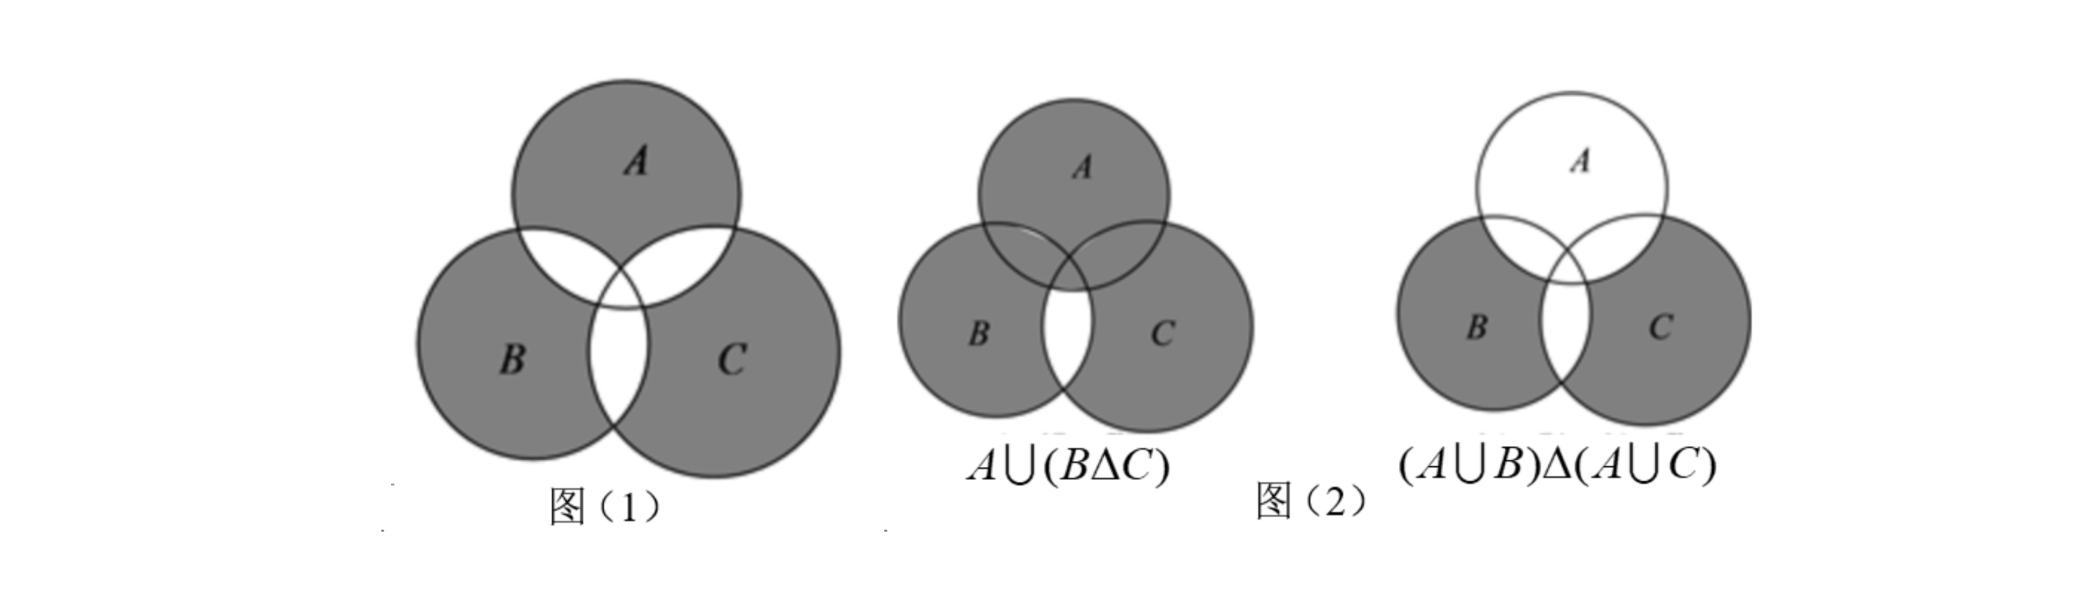
\includegraphics[width=0.92\textwidth]{figures/gao73_q16_symdiff.png}
\end{center}
\step{故选 $B$.}
\solend
\fi

\end{enumerate}

\bigsec{三、解答题}

\begin{enumerate}
\setcounter{enumi}{16}

\item （1）解不等式 $\dfrac{2-x}{x+3}>1$；

（2）已知 $a$ 是实数，试解关于 $x$ 的不等式：$x^2+(a-1)x-a\geqslant0$.

\ifanswer
\solbegin
\stepm{(1)}{$\dfrac{2-x}{x+3}-1=\dfrac{-2x-1}{x+3}>0$，则 $(2x+1)(x+3)<0$，得 $-3<x<-\dfrac12$，}
\step{所以不等式解集为 $\left(-3,-\dfrac12\right)$；}
\stepm{(2)}{$x^2+(a-1)x-a=(x+a)(x-1)\geqslant0$，}
% 原卷 (2) 题干为 ≥0，但解析按 ≤0 给出“两根之间”的解集，照录（见文件头“原卷笔误/存疑”②）
\step{当 $-a<1$，即 $a>-1$ 时，解集为 $(-a,1)$；}
\step{当 $-a=1$，即 $a=-1$ 时，解集为 $\R$；}
\step{当 $-a>1$，即 $a<-1$ 时，解集为 $(1,-a)$；}
\step{综上，当 $a>-1$ 时，解集为 $(-a,1)$；}
\step{当 $a=-1$ 时，解集为 $\R$；}
\step{当 $a<-1$ 时，解集为 $(1,-a)$.}
\solend
\fi

\ansspace[5]

\item （1）设 $a$、$b$ 是两个正数. 已知 $a>b$，比较 $\dfrac{2a+b}{a+2b}$ 与 $\dfrac ab$ 的值的大小；

（2）若实数 $a$ 满足 $\sqrt{(2023-a)^2}+\sqrt{a-2024}=a$，求 $a-2023^2$ 的值.

\ifanswer
\solbegin
\stepm{(1)}{$\dfrac{2a+b}{a+2b}-\dfrac ab=\dfrac{b^2-a^2}{b(a+2b)}<0$，所以 $\dfrac{2a+b}{a+2b}<\dfrac ab$.}
\stepm{(2)}{因为 $a-2024\geqslant0$，所以 $a\geqslant2024$，}
\step{所以 $\sqrt{(2023-a)^2}+\sqrt{a-2024}=a-2023+\sqrt{a-2024}$，}
\step{即 $a-2023+\sqrt{a-2024}=a$，即 $\sqrt{a-2024}=2023$，}
\step{所以 $a-2024=2023^2$，所以 $a-2023^2=2024$.}
\solend
\fi

\ansspace[5]

\item 已知 $m\in\R$，集合 $A=\{x\mid-1\leqslant x\leqslant3\}$，$B=\{x\mid m-3<x\leqslant m+2\}$.

（1）若“$x\in A$”是“$x\in B$”的充分不必要条件，求 $m$ 的取值范围；

（2）若 $A\cap B\neq\varnothing$，求 $m$ 的取值范围.

\ifanswer
\solbegin
\stepm{(1)}{因为“$x\in A$”是“$x\in B$”的充分不必要条件，所以 $A$ 是 $B$ 的真子集，}
\step{需满足 $\begin{cases}m-3<-1\\ m+2\geqslant3\end{cases}$，解得 $\begin{cases}m<2\\ m\geqslant1\end{cases}$，所以 $m$ 的取值范围是 $[1,2)$.}
\stepm{(2)}{因为 $A\cap B\neq\varnothing$，所以 $\begin{cases}m+2\geqslant-1\\ m-3<3\end{cases}$，解得 $\begin{cases}m\geqslant-3\\ m<6\end{cases}$，}
\step{所以 $m$ 的取值范围是 $[-3,6)$.}
\solend
\fi

\ansspace[6]

\item 已知集合 $A=\{x\mid x<-2\text{ 或 }x\geqslant3\}$，$U=\R$.

（1）若 $B=\{x\mid mx-1>0\}$，当 $B\subseteq A$ 时，求实数 $m$ 的取值范围；

（2）若 $B=\{x\mid2m-6\leqslant x\leqslant m+4\}$，当 $B\cap\overline A=\varnothing$ 时，求实数 $m$ 的取值范围.

\ifanswer
\solbegin
\stepm{(1)}{当 $m=0$ 时，$B=\varnothing$，符合题意，}
\step{当 $m>0$ 时，$B=\left\{x\mid x>\dfrac1m\right\}$，则 $\dfrac1m\geqslant3$，解得 $0<m\leqslant\dfrac13$，}
\step{当 $m<0$ 时，$B=\left\{x\mid x<\dfrac1m\right\}$，则 $\dfrac1m\leqslant-2$，解得 $-\dfrac12\leqslant m<0$，}
\step{综上所述，实数 $m$ 的取值范围 $\left[-\dfrac12,\dfrac13\right]$；}
\stepm{(2)}{由题意得 $B=\{x\mid2m-6\leqslant x\leqslant m+4\}$，$\overline A=\{x\mid-2\leqslant x<3\}$，且 $B\cap\overline A=\varnothing$，}
\step{当 $B=\varnothing$ 时，$2m-6>m+4$，解得 $m>10$，}
\step{当 $B\neq\varnothing$ 时，$\begin{cases}2m-6\leqslant m+4\\ m+4<-2\end{cases}$ 或 $\begin{cases}2m-6\leqslant m+4\\ 2m-6\geqslant3\end{cases}$，解得 $m<-6$ 或 $\dfrac92\leqslant m\leqslant10$，}
\step{综上所述，实数 $m$ 的取值范围为 $(-\infty,-6)\cup\left[\dfrac92,+\infty\right)$.}
\solend
\fi

\ansspace[7]

\item 关于实数大小关系的基本事实是解决等式或不等式问题的逻辑基础. 两个正数的大小关系是完全确定的，但通过运算就会产生非常奇妙的变化，基本不等式就是其中之一. 通过运算（代数变形）可以解决很多关于基本不等式的问题.

例如此题：正实数 $x$、$y$，满足 $x+y=1$，求 $\dfrac1x+\dfrac4y$ 的最小值. 求解本问题的方法很多，其中一种求解方法是：$\dfrac1x+\dfrac4y=(x+y)\left(\dfrac1x+\dfrac4y\right)=5+\dfrac yx+\dfrac{4x}{y}\geqslant5+2\sqrt{\dfrac yx\cdot\dfrac{4x}{y}}=9$，当且仅当 $\dfrac yx=\dfrac{4x}{y}$ 即 $y=2x$ 且 $x+y=1$ 时，即 $x=\dfrac13$，$y=\dfrac23$ 时等号成立.

这种解题方法叫作“$1$”的代换，利用上述求解方法解决下列问题：

（1）正数 $a$、$b$ 满足 $a+b=1$，求 $\dfrac1a+\dfrac2b$ 的最小值；

（2）已知 $a$、$b$、$c$ 均为正实数，且 $\dfrac1a+\dfrac1b+\dfrac1c=1$，求证：$a+b+c\geqslant9$；

（3）已知 $a$、$b$、$x$、$y$ 均为正实数，且 $\dfrac{x^2}{a^2}-\dfrac{y^2}{b^2}=1$，求证：$a^2-b^2\leqslant(x-y)^2$.

\ifanswer
\solbegin
\stepm{(1)}{正数 $a$、$b$ 满足 $a+b=1$，}
\step{$\dfrac1a+\dfrac2b=(a+b)\left(\dfrac1a+\dfrac2b\right)=1+2+\dfrac ba+\dfrac{2a}{b}\geqslant3+2\sqrt{\dfrac ba\cdot\dfrac{2a}{b}}=3+2\sqrt2$，}
\step{当且仅当 $\dfrac ba=\dfrac{2a}{b}$ 即 $b=\sqrt2\,a$ 且 $a+b=1$ 时，}
\step{即 $a=\sqrt2-1$，$b=2-\sqrt2$ 时取等号.}
\stepm{(2)}{$a+b+c=\left(\dfrac1a+\dfrac1b+\dfrac1c\right)(a+b+c)=3+\dfrac ba+\dfrac ab+\dfrac ca+\dfrac ac+\dfrac cb+\dfrac bc$}
\step{$\geqslant3+2\sqrt{\dfrac ba\cdot\dfrac ab}+2\sqrt{\dfrac ca\cdot\dfrac ac}+2\sqrt{\dfrac cb\cdot\dfrac bc}=9$，当且仅当 $a=b=c=3$ 时取等号，}
\step{故 $a+b+c\geqslant9$.}
\stepm{(3)}{$a^2-b^2=(a^2-b^2)\left(\dfrac{x^2}{a^2}-\dfrac{y^2}{b^2}\right)=x^2+y^2-\dfrac{b^2x^2}{a^2}-\dfrac{a^2y^2}{b^2}$}
\step{$=x^2+y^2-\left(\dfrac{b^2x^2}{a^2}+\dfrac{a^2y^2}{b^2}\right)\leqslant x^2+y^2-2\cdot\dfrac{bx}{a}\cdot\dfrac{ay}{b}=x^2+y^2-2xy$}
\step{$=(x-y)^2$，当且仅当 $\dfrac{bx}{a}=\dfrac{ay}{b}$ 且 $\dfrac{x^2}{a^2}-\dfrac{y^2}{b^2}=1$ 时，}
\step{即 $x=\dfrac{a^2}{\sqrt{a^2-b^2}}$，$y=\dfrac{b^2}{\sqrt{a^2-b^2}}$，$a>b$ 时取等号，故 $a^2-b^2\leqslant(x-y)^2$.}
\solend
\fi

\ansspace*[7]

\end{enumerate}

\end{document}
"
%
% 原始材料：微信公众号“魔都数学加油站”文章，连载“27学年高一73”；
% 原文标题“27学年高一73——2026-2027年上海市徐汇中学高一上10月月考”；
% 原文链接：https://mp.weixin.qq.com/s/Pkk9tFr4qHS9BR_BPxvk6A。
% 页面标注发布时间 2026-10-21 20:41（上海）。
% 正文为 10 张 PNG 页（`原图/高一73_徐汇中学_10月月考/01..10.png`）：
% 第 1、4、6、9、10 页为 2560×3620，其余 5 页为 4762×6735，均按页序读取。
% 10 页全为试卷正文页（卷首标题在第 1 页页顶，卷末第 21 题 (3) 解析止于第 10 页），
% 无封面页、目录页、二维码或宣传页。粉色斜排“魔都数学加油站”为卷面水印，未录入。
%
% 卷首标题：照卷面印作“2026-2027 年徐汇中学高一上 10 月月考”（黑体加粗一行）。
% 原卷年份区间用半角连字符，本稿按全稿惯例排 en dash；原卷无副标题。
%
% 篇幅与题号：原卷自第 3 题起编号（第 1、2 题不在本卷内）。填空题 3—12（10 题）、
% 选择题 13—16（4 题）、解答题 17—21（5 题），共 19 题。本稿沿用原节与原题号，
% 只改排为全稿统一的大节样式。
%
% 讲评版：原卷第 3、4 题只印【答案】（“没有实数根”“真”），本稿只给 \ans{}；
% 其余 17 题均印【解析】，用 \solbegin…\solend。四道选择题的作答括号原卷即留空，
% 答案写在解析末句“故选 A／D／A／B”，照录在解析内，不另提 \ans{}。
%
% 副标题：原卷未印副标题。本稿按“知识模块”口径标作“集合与常用逻辑用语、不等式”：
% 19 题中集合与常用逻辑用语 9 题（第 3、4、7、11、12、13、16、19、20 题），
% 不等式 10 题（第 5、6、8、9、10、14、15、17、18、21 题），两类均确有分量，故并标。
% 口径同 高一63、高一68—72。
%
% 与原卷的排版差异：
%   ① 原卷每题下直接印【答案】/【解析】，本稿按全稿惯例将答案与解析置于答案版；
%   ② 原卷未印副标题，本稿按“知识模块”口径补出；
%   ③ 原卷填空横线约四个字宽，本稿按全稿惯例统一排 \blankline[4.4em]；
%   ④ 原卷数集记号排斜体 $R$（第 3、8、9、10、12、17、19、20 题等），本稿按全稿惯例
%      改用 $\R$（同 高一68—72）；空集记号原卷作 $\varnothing$，照录；
%   ⑤ 原卷句末标点多为西文句点，第 15 题题干“整数解只有 $-2$”后为全角逗号，
%      均逐处照录；第 16 题解析的集合运算用 $\Delta$ 表示对称差，照原卷符号排；
%   ⑥ 第 17—21 题的子问原卷印作“（1）…（2）…”，本稿按 高一69—72 成例用行内
%      “（1）（2）（3）”段，解析中的子问标号用 \stepm{(1)}{…}；
%   ⑦ 每道解答题原卷未留作答空白，本稿按全稿惯例加 \ansspace（末题用 \ansspace*）；
%   ⑧ 选择题的作答括号原卷排半角“(    )”，本稿按全稿惯例排 \mbox{（\quad）}；
%      选项行排照原卷——第 13 题一行四条、第 14—16 题一行四条；
%   ⑨ 第 15 题题干的不等式组、第 14、19、20 题解析中的不等式组，原卷均排作“{”
%      连接的多行式，本稿按全稿惯例排 cases；
%   ⑩ 第 16 题解析末尾有三幅韦恩图（图（1）与图（2）的两幅）：原卷印在【解析】中，
%      题干无“如图”二字。本稿按原卷截图裁取（`figures/gao73_q16_symdiff.png`，
%      由第 6 页原图裁出、去除粉色水印后转灰度，未放大），放在答案版解析④之后。
%
% 原卷笔误/存疑（均照录未改，正文对应处另有 % 注）：
%   ① 第 3 题题干“设 $a$、$b\in\R$，则方程 $x^2+ax+a-1=0$ 至少有一个实根”中
%      $b$ 未在方程或后文出现，疑为衍字；原卷如此，照录未改。
%   ② 第 17 题 (2) 题干为 $x^2+(a-1)x-a\geqslant0$，但解析按 $\leqslant0$ 给出解集：
%      $a>-1$ 时写 $(-a,1)$、$a<-1$ 时写 $(1,-a)$，恰是“两根之间”的区间。
%      按题干 $\geqslant0$ 应为 $(-\infty,-a]\cup[1,+\infty)$ 与 $(-\infty,1]\cup[-a,+\infty)$；
%      原卷如此，照录未改。
%
% 行数核对：逐题数 \step/\stepm 条数与原卷【解析】印刷行数，17 题逐一相符，
% 合计 104 条 / 104 行（Q5：1；Q6：2；Q7：4；Q8：4；Q9：3；Q10：4；Q11：8；
% Q12：7；Q13：7；Q14：5；Q15：7；Q16：15；Q17：9；Q18：5；Q19：4；Q20：8；Q21：11）。
% 另第 3、4 题只印【答案】，各提 \ans{}，不计入 \step 账。
%
% 插图：第 16 题解析末的 3 幅韦恩图，见上⑩；全卷题干无其他配图。
%
\documentclass[a4paper,11pt]{article}
\usepackage{common}

\begin{document}

\examtitlest[3]{2026--2027 年徐汇中学高一上 10 月月考}{集合与常用逻辑用语、不等式}

\bigsec{一、填空题}

\begin{enumerate}
\setcounter{enumi}{2}

% 原卷题干“设 a、b∈R”中的 b 未在方程中出现，照录（见文件头“原卷笔误/存疑”①）
\item 如果用反证法证明命题“设 $a$、$b\in\R$，则方程 $x^2+ax+a-1=0$ 至少有一个实根”，那么首先假设方程 $x^2+ax+a-1=0$\blankline[4.4em].

\ifanswer
\ans{没有实数根}
\fi

\item 命题“若 $\dfrac1x>1$，则 $x<1$”是\blankline[4.4em]命题（填“真”，“假”）.

\ifanswer
\ans{真}
\fi

\item 对数 $\log_a(5-a)$ 中实数 $a$ 的取值范围是\blankline[4.4em].

\ifanswer
\solbegin
\step{由对数定义得 $\begin{cases}a>0\\ a\neq1\\ 5-a>0\end{cases}$，解得 $0<a<1$ 或 $1<a<5$.}
\solend
\fi

\item 关于 $x$ 的不等式 $ax^2-(a+1)x+1\leqslant0\,(a<0)$ 的解集为\blankline[4.4em].

\ifanswer
\solbegin
\step{原不等式即 $(ax-1)(x-1)\leqslant0$，因为 $a<0$，所以 $\left(x-\dfrac1a\right)(x-1)\geqslant0$.}
\step{又 $\dfrac1a<0<1$，所以 $x\leqslant\dfrac1a$ 或 $x\geqslant1$，故解集为 $\left(-\infty,\dfrac1a\right]\cup[1,+\infty)$.}
\solend
\fi

\item 若集合 $A=\{x\mid x^2-2kx+7k=0\}$ 有且仅有三个真子集，则 $k$ 的取值范围是\blankline[4.4em].

\ifanswer
\solbegin
\step{因为集合 $A$ 有且仅有三个真子集，则 $2^n-1=3$，解得 $n=2$，}
\step{所以一元二次方程 $x^2-2kx+7k=0$ 有两个不同的实数解，}
\step{则 $\Delta=4k^2-28k>0$，解得 $k<0$ 或 $k>7$，}
\step{故 $k$ 的取值范围是 $(-\infty,0)\cup(7,+\infty)$.}
\solend
\fi

\item 已知关于 $x$ 的不等式 $kx^2-4kx+k-6<0$ 对任意 $x\in\R$ 恒成立，则 $k$ 的取值范围是\blankline[4.4em].

\ifanswer
\solbegin
\step{关于 $x$ 的不等式 $kx^2-4kx+k-6<0$ 对任意 $x\in\R$ 恒成立，}
\step{当 $k=0$ 时，$kx^2-4kx+k-6=-6<0$ 恒成立，}
\step{当 $k\neq0$ 时，则 $\begin{cases}\Delta=16k^2-4k(k-6)<0\\ k<0\end{cases}$，解得 $-2<k<0$，}
\step{综上，$k$ 的取值范围为 $(-2,0]$.}
\solend
\fi

\item 设 $x\in\R$，方程 $|x-1|+|2x-1|=|3x-2|$ 的解集为\blankline[4.4em].

\ifanswer
\solbegin
\step{因为 $|x-1|+|2x-1|\geqslant|(x-1)+(2x-1)|=|3x-2|$，}
\step{当且仅当 $(x-1)(2x-1)\geqslant0$，解得 $x\leqslant\dfrac12$ 或 $x\geqslant1$，}
\step{故方程 $|x-1|+|2x-1|=|3x-2|$ 的解集为 $\left(-\infty,\dfrac12\right]\cup[1,+\infty)$.}
\solend
\fi

\item 已知 $a\in\R$，若关于 $x$ 的方程 $x^2+ax+a^2-8=0$ 有两个实根 $x_1$、$x_2$，且 $\dfrac1{x_1}+\dfrac1{x_2}=-\dfrac12$，则 $a$ 的值为\blankline[4.4em].

\ifanswer
\solbegin
\step{由题意得 $\Delta=a^2-4(a^2-8)=32-3a^2\geqslant0$，解得 $a^2\leqslant\dfrac{32}3$，}
\step{由韦达定理得 $x_1+x_2=-a$，$x_1x_2=a^2-8$，}
\step{则 $\dfrac1{x_1}+\dfrac1{x_2}=\dfrac{x_1+x_2}{x_1x_2}=\dfrac{-a}{a^2-8}=-\dfrac12$，即 $a^2-2a-8=(a-4)(a+2)=0$，}
\step{解得 $a=4$ 或 $a=-2$. 又 $a^2\leqslant\dfrac{32}3$，则 $a=-2$.}
\solend
\fi

\item 甲、乙两人解关于 $x$ 的不等式 $x^2+bx+c<0$，甲写错了 $b$，正确计算后得到的解为 $\{x\mid1<x<2\}$；乙写错了 $c$，正确计算后得到的解为 $\{x\mid-4<x<1\}$. 那么不等式 $\dfrac{bx+c}{x-2}<0$ 的解为\blankline[4.4em].

\ifanswer
\solbegin
\step{由 $x^2+bx+c<0$ 的解为 $\{x\mid1<x<2\}$，}
\step{则 $1$ 和 $2$ 是方程 $x^2+bx+c=0$ 的两个根，}
\step{甲写错了 $b$，但 $c$ 是正确的，所以 $c=1\times2=2$；}
\step{由 $x^2+bx+c<0$ 的解为 $\{x\mid-4<x<1\}$，}
\step{则 $-4$ 和 $1$ 是方程 $x^2+bx+c=0$ 的两个根，}
\step{乙写错了 $c$，但 $b$ 是正确的，所以 $-b=-4+1=-3$，即 $b=3$.}
\step{由 $\dfrac{bx+c}{x-2}<0$，得 $\dfrac{3x+2}{x-2}<0$，即 $(3x+2)(x-2)<0$，解得 $-\dfrac23<x<2$，}
\step{所以不等式 $\dfrac{bx+c}{x-2}<0$ 的解为 $\left\{x\mid-\dfrac23<x<2\right\}$.}
\solend
\fi

\item 设 $a,b,c\in\R$，$S=\{x\mid(x+a)(x^2+bx+c)=0,x\in\R\}$，$T=\{x\mid(ax+1)(cx^2+bx+1)=0,x\in\R\}$. 若 $|S|$、$|T|$ 分别为集合 $S$、$T$ 的元素个数，则 $|S|+|T|$ 的所有可能取值组成的集合为\blankline[4.4em].

\ifanswer
\solbegin
\step{$x\neq0$ 时，$(ax+1)(cx^2+bx+1)=x^3\left(\dfrac1x+a\right)\left(\dfrac1{x^2}+\dfrac bx+c\right)$，}
\step{故 $S$、$T$ 的非零元按倒数一一对应，设其个数均为 $k$；}
\step{$0\notin T$，且 $0\in S\Leftrightarrow ac=0$. 当 $ac=0$ 时 $k\in\{0,1,2\}$，}
\step{当 $ac\neq0$ 时 $x=-a\neq0$ 是 $S$ 的非零元，$k\in\{1,2,3\}$.}
\step{因此 $|S|+|T|$ 分别可取 $2k+1\in\{1,3,5\}$ 与 $2k\in\{2,4,6\}$.}
\step{依次取 $(a,b,c)=(0,0,0),(1,0,1),(0,-2,1),(1,-2,1),(0,0,-1),(1,-5,6)$，可分别实现 $1,2,3,4,5,6$，}
\step{则 $|S|+|T|$ 的所有可能取值组成的集合为 $\{1,2,3,4,5,6\}$.}
\solend
\fi

\end{enumerate}

\bigsec{二、选择题}

\begin{enumerate}
\setcounter{enumi}{12}

\item 如果 $a>b$，$c\neq0$，那么下列不等式成立的是\mbox{（\quad）}

\keepwithprev
A. $a-c>b-c$\qquad B. $c-a>c-b$\qquad C. $ac>bc$\qquad D. $\dfrac ac>\dfrac bc$

\ifanswer
\solbegin
\step{对于 $A$：$a-c-(b-c)=a-b>0$，即 $a-c>b-c$，故 $A$ 正确；}
\step{对于 $B$：$c-a-(c-b)=b-a<0$，即 $c-a<c-b$，故 $B$ 错误；}
\step{对于 $C$：$ac-bc=c(a-b)$，已知 $a-b>0$，}
\step{当 $c<0$ 时，$c(a-b)<0$，此时 $ac<bc$，故 $C$ 错误；}
\step{对于 $D$：$\dfrac ac-\dfrac bc=\dfrac1c(a-b)$，已知 $a-b>0$，}
\step{当 $c<0$ 时，$\dfrac1c(a-b)<0$，此时 $\dfrac ac<\dfrac bc$，故 $D$ 错误.}
\step{故选 $A$.}
\solend
\fi

\item 若不等式 $|x+1|\leqslant a$ 成立的一个充分不必要条件是 $-3\leqslant x\leqslant4$，则整数 $a$ 的最小值为\mbox{（\quad）}

\keepwithprev
A. $2$\qquad B. $3$\qquad C. $4$\qquad D. $5$

\ifanswer
\solbegin
\step{若 $a<0$，则 $|x+1|\leqslant a$ 无解；}
\step{若 $a\geqslant0$，由 $|x+1|\leqslant a$，得 $-1-a\leqslant x\leqslant-1+a$，}
\step{因为 $|x+1|\leqslant a$ 成立的一个充分不必要条件是 $-3\leqslant x\leqslant4$，}
\step{所以 $\begin{cases}-1-a\leqslant-3\\ -1+a\geqslant4\end{cases}$，等号不同时成立，解得 $a\geqslant5$，}
\step{故整数 $a$ 的最小值为 $5$. 故选 $D$.}
\solend
\fi

\item 若关于 $x$ 的不等式组 $\begin{cases}x^2-x-2>0\\ 2x^2+(5+2k)x+5k<0\end{cases}$ 的整数解只有 $-2$，则实数 $k$ 的取值范围为\mbox{（\quad）}

\keepwithprev
A. $[-3,2)$\qquad B. $[1,2]$\qquad C. $(1,2]$\qquad D. $(1,2)$

\ifanswer
\solbegin
\step{由 $x^2-x-2>0$，得 $x>2$ 或 $x<-1$，}
\step{由 $2x^2+(2k+5)x+5k<0$，得 $(2x+5)(x+k)<0$.}
\step{①若 $-k<-\dfrac52$，即 $k>\dfrac52$ 时，解得 $-k<x<-\dfrac52$，}
\step{此时原不等式的解集为 $\left(-k,-\dfrac52\right)$，不符合题意；}
\step{②若 $k=\dfrac52$ 时，解得 $x\in\varnothing$，显然不符合题意；}
\step{③若 $k<\dfrac52$ 时，解得 $-\dfrac52<x<-k$，则 $-2<-k\leqslant3$，即 $-3\leqslant k<2$.}
\step{综上，实数 $k$ 的取值范围 $[-3,2)$. 故选 $A$.}
\solend
\fi

\item 定义集合运算 $A-B=\{x\mid x\in A\text{ 且 }x\notin B\}$ 称为集合 $A$ 与集合 $B$ 的差集；定义集合运算 $A\Delta B=(A-B)\cup(B-A)$ 称为集合 $A$ 与集合 $B$ 的对称差，有以下 $4$ 个等式：

① $A\Delta B=B\Delta A$；

② $(A\Delta B)\Delta C=A\Delta(B\Delta C)$；

③ $A\cap(B\Delta C)=(A\cap B)\Delta(A\cap C)$；

④ $A\cup(B\Delta C)=(A\cup B)\Delta(A\cup C)$.

则 $4$ 个等式中恒成立的是\mbox{（\quad）}

\keepwithprev
A. ①②\qquad B. ①②③\qquad C. ①②④\qquad D. ①②③④

\ifanswer
\solbegin
\step{对于①，由 $B\Delta A=(B-A)\cup(A-B)=(A-B)\cup(B-A)=A\Delta B$，}
\step{所以①正确；}
\step{对于②，}
\step{由 $A-B=\{x\mid x\in A\text{ 且 }x\notin B\}=\{x\mid x\in A,x\notin(A\cap B)\}=A-(A\cap B)$，}
\step{同理可得 $B-A=B-(A\cap B)$，}
\step{则 $A\Delta B=(A-B)\cup(B-A)=(A\cup B)-(A\cap B)$，}
\step{所以 $(A\Delta B)\Delta C=(A\Delta B)\cup C-(A\Delta B)\cap C$，}
\step{所以表示的集合为图（1）中阴影部分所表示的集合，如图所示，}
\step{同理 $A\Delta(B\Delta C)=A\cup(B\Delta C)-A\cap(B\Delta C)$，}
\step{也表示图（1）中阴影部分所表示的集合，}
\step{所以 $(A\Delta B)\Delta C=A\Delta(B\Delta C)$，所以②正确；}
\step{对于③，由 $A\cap(B\Delta C)=A\cap(B\cup C-B\cap C)=A\cap(B\cup C)-A\cap(B\cap C)$}
\step{$=(A\cap B)\cup(A\cap C)-(A\cap B)\cap(A\cap C)=(A\cap B)\Delta(A\cap C)$，所以③正确；}
\step{对于④，如图（2）所示，$A\cup(B\Delta C)\neq(A\cup B)\Delta(A\cup C)$，所以④错误.}
\begin{center}
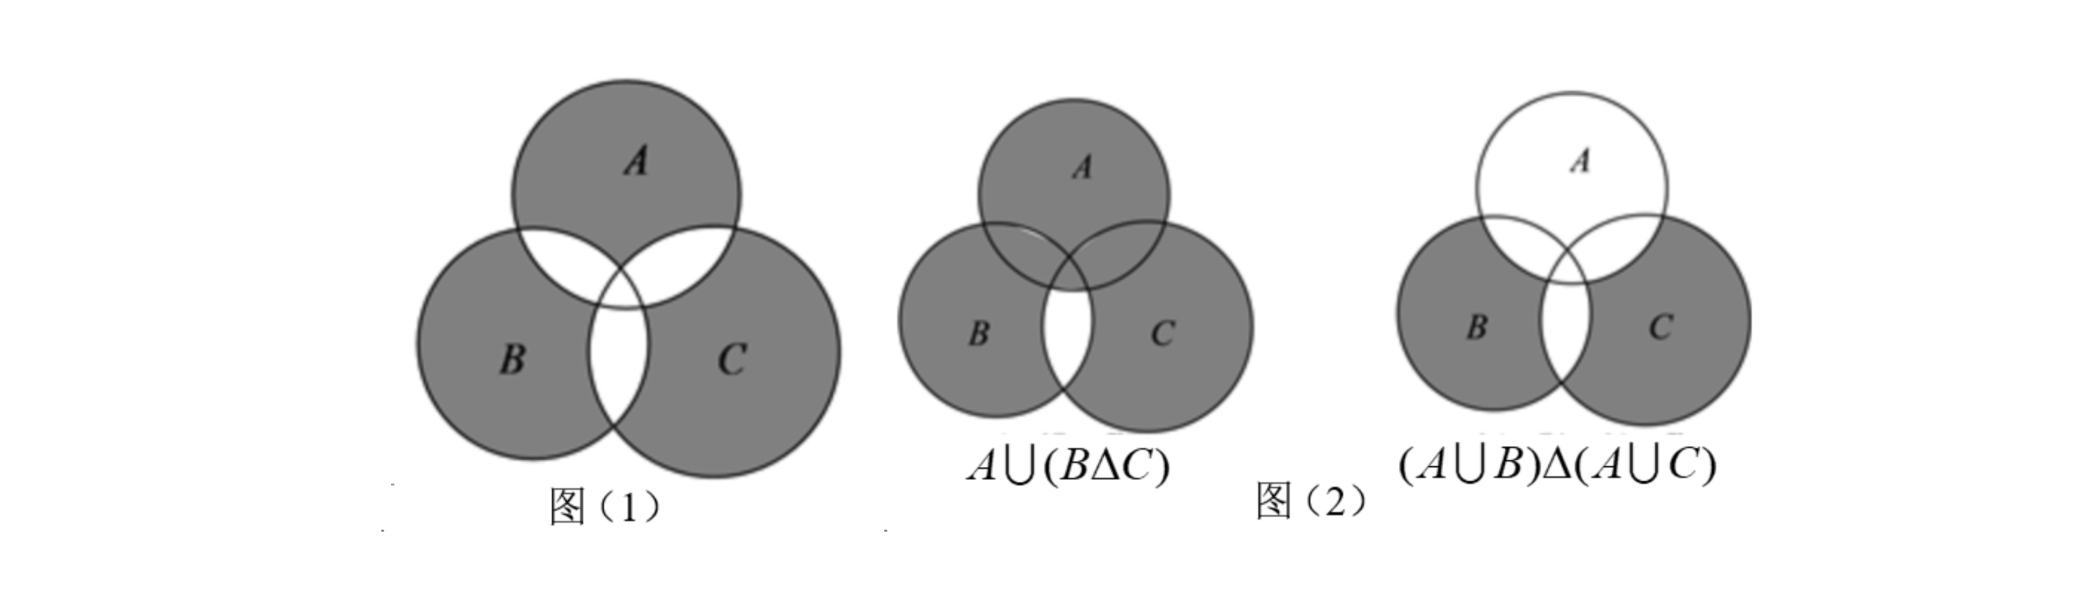
\includegraphics[width=0.92\textwidth]{figures/gao73_q16_symdiff.png}
\end{center}
\step{故选 $B$.}
\solend
\fi

\end{enumerate}

\bigsec{三、解答题}

\begin{enumerate}
\setcounter{enumi}{16}

\item （1）解不等式 $\dfrac{2-x}{x+3}>1$；

（2）已知 $a$ 是实数，试解关于 $x$ 的不等式：$x^2+(a-1)x-a\geqslant0$.

\ifanswer
\solbegin
\stepm{(1)}{$\dfrac{2-x}{x+3}-1=\dfrac{-2x-1}{x+3}>0$，则 $(2x+1)(x+3)<0$，得 $-3<x<-\dfrac12$，}
\step{所以不等式解集为 $\left(-3,-\dfrac12\right)$；}
\stepm{(2)}{$x^2+(a-1)x-a=(x+a)(x-1)\geqslant0$，}
% 原卷 (2) 题干为 ≥0，但解析按 ≤0 给出“两根之间”的解集，照录（见文件头“原卷笔误/存疑”②）
\step{当 $-a<1$，即 $a>-1$ 时，解集为 $(-a,1)$；}
\step{当 $-a=1$，即 $a=-1$ 时，解集为 $\R$；}
\step{当 $-a>1$，即 $a<-1$ 时，解集为 $(1,-a)$；}
\step{综上，当 $a>-1$ 时，解集为 $(-a,1)$；}
\step{当 $a=-1$ 时，解集为 $\R$；}
\step{当 $a<-1$ 时，解集为 $(1,-a)$.}
\solend
\fi

\ansspace[5]

\item （1）设 $a$、$b$ 是两个正数. 已知 $a>b$，比较 $\dfrac{2a+b}{a+2b}$ 与 $\dfrac ab$ 的值的大小；

（2）若实数 $a$ 满足 $\sqrt{(2023-a)^2}+\sqrt{a-2024}=a$，求 $a-2023^2$ 的值.

\ifanswer
\solbegin
\stepm{(1)}{$\dfrac{2a+b}{a+2b}-\dfrac ab=\dfrac{b^2-a^2}{b(a+2b)}<0$，所以 $\dfrac{2a+b}{a+2b}<\dfrac ab$.}
\stepm{(2)}{因为 $a-2024\geqslant0$，所以 $a\geqslant2024$，}
\step{所以 $\sqrt{(2023-a)^2}+\sqrt{a-2024}=a-2023+\sqrt{a-2024}$，}
\step{即 $a-2023+\sqrt{a-2024}=a$，即 $\sqrt{a-2024}=2023$，}
\step{所以 $a-2024=2023^2$，所以 $a-2023^2=2024$.}
\solend
\fi

\ansspace[5]

\item 已知 $m\in\R$，集合 $A=\{x\mid-1\leqslant x\leqslant3\}$，$B=\{x\mid m-3<x\leqslant m+2\}$.

（1）若“$x\in A$”是“$x\in B$”的充分不必要条件，求 $m$ 的取值范围；

（2）若 $A\cap B\neq\varnothing$，求 $m$ 的取值范围.

\ifanswer
\solbegin
\stepm{(1)}{因为“$x\in A$”是“$x\in B$”的充分不必要条件，所以 $A$ 是 $B$ 的真子集，}
\step{需满足 $\begin{cases}m-3<-1\\ m+2\geqslant3\end{cases}$，解得 $\begin{cases}m<2\\ m\geqslant1\end{cases}$，所以 $m$ 的取值范围是 $[1,2)$.}
\stepm{(2)}{因为 $A\cap B\neq\varnothing$，所以 $\begin{cases}m+2\geqslant-1\\ m-3<3\end{cases}$，解得 $\begin{cases}m\geqslant-3\\ m<6\end{cases}$，}
\step{所以 $m$ 的取值范围是 $[-3,6)$.}
\solend
\fi

\ansspace[6]

\item 已知集合 $A=\{x\mid x<-2\text{ 或 }x\geqslant3\}$，$U=\R$.

（1）若 $B=\{x\mid mx-1>0\}$，当 $B\subseteq A$ 时，求实数 $m$ 的取值范围；

（2）若 $B=\{x\mid2m-6\leqslant x\leqslant m+4\}$，当 $B\cap\overline A=\varnothing$ 时，求实数 $m$ 的取值范围.

\ifanswer
\solbegin
\stepm{(1)}{当 $m=0$ 时，$B=\varnothing$，符合题意，}
\step{当 $m>0$ 时，$B=\left\{x\mid x>\dfrac1m\right\}$，则 $\dfrac1m\geqslant3$，解得 $0<m\leqslant\dfrac13$，}
\step{当 $m<0$ 时，$B=\left\{x\mid x<\dfrac1m\right\}$，则 $\dfrac1m\leqslant-2$，解得 $-\dfrac12\leqslant m<0$，}
\step{综上所述，实数 $m$ 的取值范围 $\left[-\dfrac12,\dfrac13\right]$；}
\stepm{(2)}{由题意得 $B=\{x\mid2m-6\leqslant x\leqslant m+4\}$，$\overline A=\{x\mid-2\leqslant x<3\}$，且 $B\cap\overline A=\varnothing$，}
\step{当 $B=\varnothing$ 时，$2m-6>m+4$，解得 $m>10$，}
\step{当 $B\neq\varnothing$ 时，$\begin{cases}2m-6\leqslant m+4\\ m+4<-2\end{cases}$ 或 $\begin{cases}2m-6\leqslant m+4\\ 2m-6\geqslant3\end{cases}$，解得 $m<-6$ 或 $\dfrac92\leqslant m\leqslant10$，}
\step{综上所述，实数 $m$ 的取值范围为 $(-\infty,-6)\cup\left[\dfrac92,+\infty\right)$.}
\solend
\fi

\ansspace[7]

\item 关于实数大小关系的基本事实是解决等式或不等式问题的逻辑基础. 两个正数的大小关系是完全确定的，但通过运算就会产生非常奇妙的变化，基本不等式就是其中之一. 通过运算（代数变形）可以解决很多关于基本不等式的问题.

例如此题：正实数 $x$、$y$，满足 $x+y=1$，求 $\dfrac1x+\dfrac4y$ 的最小值. 求解本问题的方法很多，其中一种求解方法是：$\dfrac1x+\dfrac4y=(x+y)\left(\dfrac1x+\dfrac4y\right)=5+\dfrac yx+\dfrac{4x}{y}\geqslant5+2\sqrt{\dfrac yx\cdot\dfrac{4x}{y}}=9$，当且仅当 $\dfrac yx=\dfrac{4x}{y}$ 即 $y=2x$ 且 $x+y=1$ 时，即 $x=\dfrac13$，$y=\dfrac23$ 时等号成立.

这种解题方法叫作“$1$”的代换，利用上述求解方法解决下列问题：

（1）正数 $a$、$b$ 满足 $a+b=1$，求 $\dfrac1a+\dfrac2b$ 的最小值；

（2）已知 $a$、$b$、$c$ 均为正实数，且 $\dfrac1a+\dfrac1b+\dfrac1c=1$，求证：$a+b+c\geqslant9$；

（3）已知 $a$、$b$、$x$、$y$ 均为正实数，且 $\dfrac{x^2}{a^2}-\dfrac{y^2}{b^2}=1$，求证：$a^2-b^2\leqslant(x-y)^2$.

\ifanswer
\solbegin
\stepm{(1)}{正数 $a$、$b$ 满足 $a+b=1$，}
\step{$\dfrac1a+\dfrac2b=(a+b)\left(\dfrac1a+\dfrac2b\right)=1+2+\dfrac ba+\dfrac{2a}{b}\geqslant3+2\sqrt{\dfrac ba\cdot\dfrac{2a}{b}}=3+2\sqrt2$，}
\step{当且仅当 $\dfrac ba=\dfrac{2a}{b}$ 即 $b=\sqrt2\,a$ 且 $a+b=1$ 时，}
\step{即 $a=\sqrt2-1$，$b=2-\sqrt2$ 时取等号.}
\stepm{(2)}{$a+b+c=\left(\dfrac1a+\dfrac1b+\dfrac1c\right)(a+b+c)=3+\dfrac ba+\dfrac ab+\dfrac ca+\dfrac ac+\dfrac cb+\dfrac bc$}
\step{$\geqslant3+2\sqrt{\dfrac ba\cdot\dfrac ab}+2\sqrt{\dfrac ca\cdot\dfrac ac}+2\sqrt{\dfrac cb\cdot\dfrac bc}=9$，当且仅当 $a=b=c=3$ 时取等号，}
\step{故 $a+b+c\geqslant9$.}
\stepm{(3)}{$a^2-b^2=(a^2-b^2)\left(\dfrac{x^2}{a^2}-\dfrac{y^2}{b^2}\right)=x^2+y^2-\dfrac{b^2x^2}{a^2}-\dfrac{a^2y^2}{b^2}$}
\step{$=x^2+y^2-\left(\dfrac{b^2x^2}{a^2}+\dfrac{a^2y^2}{b^2}\right)\leqslant x^2+y^2-2\cdot\dfrac{bx}{a}\cdot\dfrac{ay}{b}=x^2+y^2-2xy$}
\step{$=(x-y)^2$，当且仅当 $\dfrac{bx}{a}=\dfrac{ay}{b}$ 且 $\dfrac{x^2}{a^2}-\dfrac{y^2}{b^2}=1$ 时，}
\step{即 $x=\dfrac{a^2}{\sqrt{a^2-b^2}}$，$y=\dfrac{b^2}{\sqrt{a^2-b^2}}$，$a>b$ 时取等号，故 $a^2-b^2\leqslant(x-y)^2$.}
\solend
\fi

\ansspace*[7]

\end{enumerate}

\end{document}
